\documentclass[a4paper,10pt,oneside]{book}
\usepackage[utf8x]{inputenc}
\usepackage{hyperref}
\usepackage{amsthm,amssymb,amsmath}
\usepackage{authblk}
\usepackage[usenames,dvipsnames]{color}
\usepackage{graphicx}
\usepackage{hhline}
\usepackage{float}

\renewcommand{\bibname}{References} 
% Margin Notes on the Left
\reversemarginpar
% Margin Notes with small italics
\setlength{\marginparwidth}{1.2in}
\let\oldmarginpar\marginpar
\renewcommand\marginpar[1]{\-\oldmarginpar[\raggedleft\footnotesize\textit{ #1}]{\raggedright\footnotesize #1}}
\renewcommand\Affilfont{\itshape\small} % small font, italics for affiliations



\renewcommand\Affilfont{\itshape\small} % small font, italics for affiliations

\newtheorem{theorem}{Theorem}
\newtheorem{lemma}{Lemma}
\newtheorem{claim}{Claim}
\newtheorem{example}{Example}
\newtheorem{definition}{Definition}
\newtheorem{proposition}[theorem]{Proposition}
\newtheorem{corollary}[theorem]{Corollary}

\hypersetup{
    unicode=false,          % non-Latin characters in Acrobat’s bookmarks
    pdftoolbar=true,        % show Acrobat’s toolbar?
    pdfmenubar=true,        % show Acrobat’s menu?
    pdffitwindow=false,     % window fit to page when opened
    pdfstartview={FitH},    % fits the width of the page to the window
    pdftitle={(DRAFT) The Realm of State Space Systems (DRAFT)},    % title
    pdfauthor={Pantelis Sopasakis},     % author
    pdfsubject={State space models - theory, examples},   % subject of the document
    pdfcreator={Pantelis Sopasakis},   % creator of	 the document
    pdfproducer={}, % producer of the document
    pdfkeywords={State Space} {Controllability} {Observability}, % list of keywords
    pdfnewwindow=true,      % links in new window
    colorlinks=true,       % false: boxed links; true: colored links
    linkcolor=blue,          % color of internal links
    citecolor=	Orange,        % color of links to bibliography
    filecolor=magenta,      % color of file links
    urlcolor=	DarkOrchid           % color of external links
}


\pagestyle{plain} 

\title{The Realm of Linear State Space Control Systems\\\textit{Draft Version}}
\author{
  \href{mailto:chvng@mail.ntua.gr}{Pantelis Sopasakis}
}
\affil{Dipl. Chem. Eng., Msc. Appl. Math.,\\National Technical University of Athens}


\begin{document}
\maketitle

\chapter*{Preface}
Usually, the starting point for the study of Automatic Control 
is the \emph{Laplace Space} of the complex variable $s\in\mathbb{C}$,
sometimes referred to as the \emph{Complex Frequency Domain},
or the $\mathcal{Z}$-transform for digital systems. 
Using the Laplace transform, the differential equations that accrue 
from the various principles of mechanics or chemistry, become algebraic 
equations which can be easily manipulated. However, certain assumptions
render this approach rather restrictive. Firstly, the Laplace Transform cannot
be applied on arbitrary functions or in some cases it becomes cumbersome to
invert it. Moreover, the requirement for zero initial conditions yields a rather
stiff theory.\\
\\
The State Space approach copes directly with the differential equations of 
the system and exhibits the following advantages:

\begin{enumerate}
 \item Single Input Single Output (SISO) and Multiple Input Multiple Output (MIMO) systems are treated using the same framework. 
 \item New concepts such as Controllability and Observability are defined and studied methodologically. The state space representation is more appropriate for the theoretical study of the underlying system.
 \item Offers a better insight into the system's structure as its states are explicitly studied in contrast to a single-input single-output black box.
 \item Analytical solutions are often available. In general, numerical solution algorithms (e.g. The \href{http://en.wikipedia.org/wiki/Runge\%E2\%80\%93Kutta_methods}{Runge-Kutta algorithm})
 \item The state-space formulation is the basis for the study of nonlinear systems.
\end{enumerate}

The results outlined in these notes apply mainly to linear time-invariant systems. The author has endeavoured to provide a concise and rigorous but yet understandable presentation of some of the most interesting results in linear dynamical systems theory.

Finally, the State Space representation of dynamical systems is the basis for the modern theory of Model Predictive Control and the ubiquitous Lyapunov Theory of Stability. \\
\\
\\
Please cite these notes as follows:\\
Pantelis Sopasakis, \emph{The Realm of Linear State Space Control Systems}, 2011, Available online at \href{http://users.ntua.gr/chvng/en/}{http://users.ntua.gr/chvng/en} (Accessed on: \today).


\thispagestyle{empty} %no page number
\addtocounter{page}{-1} %ignore this page when counting
\vspace{2.5in} %start the dedication halfway down
\begin{center} %center everything
{
\emph{If two wrongs don't make a right, try three.}\\
Unknown
}

\end{center}


\tableofcontents
\chapter{Introduction}
The \href{http://en.wikipedia.org/wiki/Laplace_transform}{Laplace transform} and the use of transfer functions offer great flexibility regarding the study of a system's dynamics and stability. However, the requirement for the initial state to be the origin proves to be an important drawback. The state space approach provides a more generic framework for the study of dynamical systems. Although in what follows we will stick to the study of linear systems, state space models can be used for the representation and study of nonlinear systems and systems that are not Laplace-transformable. 
The system dynamics evolves through the \emph{state variables}:
\[\mathbf{x}(t)=[x_1(t)\ x_2(t)\ \cdots x_n(t)]'\in\mathbb{R}^n\] 
which come to the outer world of the system as \emph{output variables}: 
\[\mathbf{y}(t)=[y_1(t)\ y_2(t)\ \cdots\ y_p(t)]'=h(\mathbf{x}(t),\mathbf{u}(t))\in\mathbb{R}^p\]
where $h:\mathbb{R}^n\times\mathbb{R}^m\rightarrow\mathbb{R}^p$ is a function that defines the state-to-output behaviour of the system. Finally, let $\mathbf{u}:\mathbb{R}\ni t \mapsto \mathbf{u}(t)\in\mathbb{R}^m$ be the \emph{input variable} to the system which we assume that is a \emph{controlled variable}. In what follows we will not consider any disturbances. 

A state space model consists of two main parts which describe the input-to-state dynamics and the state-to-output relations of the underlying system. In particular these are:

\begin{enumerate}
 \item The \textbf{state equations}: They describe the dynamic relationship between the input variable $\mathbf{u}$ and the state vector $\mathbf{x}$. Usually these are ordinary differential equations of the form: $\dot{\mathbf{x}}(t) = f(t,\mathbf{x}(t),\mathbf{u}(t))$ (time-variant system) or $\dot{\mathbf{x}}(t) = f(\mathbf{x}(t),\mathbf{u}(t))$ (time-invariant system). In these notes we will study only time-invariant systems where the vector field $f:\mathbb{R}^n \times \mathbb{R}^m \rightarrow \mathbb{R}^n$ is a linear functional of the form $f(\mathbf{x},\mathbf{u})=\mathbf{Ax}+\mathbf{Bu}$ where $\mathbf{A}$ and $\mathbf{B}$ are matrices of proper dimensions.
 \item The \textbf{output equations}: Describe the state-to-output behaviour of the system through relations of the form $\mathbf{y}(t)=h(\mathbf{x}(t),\mathbf{u}(t))$.
\end{enumerate}

Overall, a state space dynamical system admits the following general realization:
\begin{eqnarray}
 \dot{\mathbf{x}}(t) = f(\mathbf{x}(t),\mathbf{u}(t))\label{stateSpace1}\\
 \mathbf{y}(t)=h(\mathbf{x}(t),\mathbf{u}(t))
\end{eqnarray}

Hereinafter we shall use the notation $\Sigma[\mathbf{x},\mathbf{u},\mathbf{y}]$ to refer to a system with state variable $\mathbf{x}$, input variable $\mathbf{u}$ and output variable $\mathbf{y}$.
The notion of an equilibrium point applies to state space models as follows:
\begin{definition}[Equilibrium point]\label{definition:equilibrium}\hypertarget{definition:equilibrium}
 A point $(\mathbf{x}^\star,\mathbf{u}^\star)\in \mathbb{R}^n \times \mathbb{R}^m$ is called an equilibrium point for (\ref{stateSpace1}) if $f(t,\mathbf{x}^\star,\mathbf{u}^\star)=0$ for all $t\in\mathbb{R}$
\end{definition}


\chapter{Classes of State Space Models}\label{classesOfModels}
First we consider of the most general form of state space systems which is \emph{nonlinear} and \emph{time-variant}. We shall refer to this class of systems as $\Sigma_{\text{G}}$. These have the following structure:
\begin{eqnarray}
 \dot{\mathbf{x}}(t) &=& f(t,\mathbf{x}(t),\mathbf{u}(t))\label{SG1}\\
 \mathbf{y}(t) &=& h(t,\mathbf{x}(t),\mathbf{u}(t))\label{SG2}
\end{eqnarray}
In what follows we use the symbols $n,m$ and $p$ respectively to refer to the dimensions of the state, the input and the output vectors; usually it is $m\leq n$ and $p\leq n$. Little can be inferred from this general representation consisting of (\ref{SG1}) and (\ref{SG2}) without any further assumptions. In most cases, state space models have a more specific structure which allows us to derive particular results. Dominantly, we have the following classes of systems according to the form of the vector fields $f$ and $h$.

\section{Linear Time Invariant Models}\hypertarget{sec:LTI}
These are models in which the vector field $f$ has the special form:
\begin{eqnarray}
 f(t,\mathbf{x},\mathbf{u})=\mathbf{Ax}(t)+\mathbf{Bu}(t)
\end{eqnarray}
Where $\mathbf{A}\in M_n(\mathbb{R})$ is a square matrix and $\mathbf{B}\in M_{n\times m}(\mathbb{R})$. The state-to-output relation is described by:
\begin{eqnarray}
 h(t,\mathbf{x},\mathbf{u})=\mathbf{Cx}(t)+\mathbf{Du}(t)
\end{eqnarray}
where $\mathbf{C}\in M_{p\times n}(\mathbb{R})$ and $\mathbf{D}\in M_{p\times m}(\mathbb{R})$ while it is quite common that $\mathbf{D}=\mathbf{0}$ therefore Linear Time-Invariant (LTI) models appear to be even simpler. An LTI system is represented as:
\begin{equation}
 \Sigma_{\text{LTI}}=\left( \mathbf{A},\mathbf{B},\mathbf{C},\mathbf{D}\right)
\end{equation}
Here is an example of an LTI system with $n=2$ and $m=p=1$:
\begin{eqnarray}
\dot{\mathbf{x}}(t)&=&\left[ {\begin{array}{cc}
 2 & 3  \\
 -1 & 1  \\
 \end{array} } \right]
\mathbf{x}(t)+ 
\left[ {\begin{array}{c}
 1  \\
 0  \\
 \end{array} } \right]
u(t)\\
\mathbf{y}(t)&=&\left[ {\begin{array}{cc}
 1 & 0  
 \end{array} } \right]\mathbf{x}(t)=x_1(t)
\end{eqnarray}
For LTI systems, according to definition \ref{definition:equilibrium}, the pair $(\mathbf{x}^\star,\mathbf{u}^\star)$ is an \hyperlink{definition:equilibrium}{equilibrium point} if $\mathbf{Ax}^\star+\mathbf{Bu}^\star=0$. If we choose $\mathbf{x}^\star=\mathbf{0}$ then the requirement becomes $\mathbf{Bu}^\star=\mathbf{0}$ or equivalently $\mathbf{u}^\star \in \operatorname{ker}\mathbf{B}$.
\section{Linear Time Variant Models}
 Linear Time-Variant (LTV) models is a more general class than the above described one of LTI systems in which the coefficients $\mathbf{A},\mathbf{B},\mathbf{C},\mathbf{D}$ can vary with time. LTV models are represented as follows:
\begin{eqnarray}
 \dot{\mathbf{x}}(t)&=&f(t,\mathbf{x}(t),\mathbf{u}(t))=\mathbf{A}(t)\mathbf{x}(t)+\mathbf{B}(t)\mathbf{u}(t)\\
 \mathbf{y}(t)&=&h(t,\mathbf{x}(t),\mathbf{u}(t))=\mathbf{C}(t)\mathbf{x}(t)+\mathbf{D}(t)\mathbf{u}(t)
\end{eqnarray}
Fruitful results arise with the assumption that these matrices are periodic functions of $t$. LTV systems will be referred to hereinafter as $\Sigma_{\text{LTV}}$.


\section{Input Affine Nonlinear Models}
In this case the function $f$ has the following form:
\begin{eqnarray}
 f(t,\mathbf{x},\mathbf{u})&=&\gamma(\mathbf{x})+\sum_{i=1}^{m}g_i(\mathbf{x})\cdot u_i(t)=\gamma(\mathbf{x})+\mathbf{g}'(\mathbf{x})\cdot\mathbf{u}
\end{eqnarray}
where $\gamma:\mathbb{R}^n\rightarrow\mathbb{R}^n$ and $\mathbf{g}:\mathbb{R}^n\rightarrow\mathbb{R}^n$ are smooth functions. These models describe a wide range of physical systems however in the most general case and without any further assumptions the derived results are only local; around a neighborhood of an equilibrium point.

\section{Bilinear Models}
Bilinear models form a subclass of input affine models particularly useful for modelling of chemical processes. Additionally they possess a simpler structure than the one of input affine models therefore one can derive richer results. Bilinear models have the form:
\begin{eqnarray}
 \dot{\mathbf{x}}(t)&=&f(t,\mathbf{x}(t),\mathbf{u}(t))=\mathbf{A}\mathbf{x}(t)+\mathbf{B}\mathbf{u}(t)+\mathbf{x}'(t)\mathbf{Su}(t)\\
 \mathbf{y}(t)&=&h(t,\mathbf{x}(t),\mathbf{u}(t))=\mathbf{C}\mathbf{x}(t)+\mathbf{D}\mathbf{u}(t)
\end{eqnarray}
where $\mathbf{S}\in M_{n\times m}(\mathbb{R})$.


\chapter{Coordinates Transformations}
A coordinate transformation is a technique used to simplify the structure of a given model and can be applied to any of the categories of chapter \ref{classesOfModels}. A \emph{coordinate transformation} or \emph{change of coordinates} is defined as follows:

\begin{definition}[Coordinates transformation]\label{def:changeOfCoordinates}\hypertarget{def:changeOfCoordinates}
 A function $\Phi:S\rightarrow S$ where $S\subseteq \mathbb{R}^n$ an open set, is called a coordinates transformation on $S$ (or a local diffeomorphism on $S$) if the following hold:
\begin{enumerate}
 \item $\Phi$ is injective, i.e. for all $y\in S$ there is a $s \in S$ such that $\Phi(s)=y$.
 \item $\Phi$ is invertible, i.e. there is a function $\Phi^{-1}$ such that $\Phi^{-1}(\Phi(x))=x$ for all $x \in S$
 \item The functions $\Phi$ and $\Phi^{-1}$ are infinitely many times differentiable.
\end{enumerate}
Additionally, if $S=\mathbb{R}^n$ is said to be a global change of coordinates.
\end{definition}


Given a system $\Sigma[\mathbf{x},\mathbf{u}]$ with state variable $x$ and input variable $u$ and with state equation:
\begin{eqnarray}
 \dot{\mathbf{x}}(t)&=&f(\mathbf{x},\mathbf{u})
\end{eqnarray}
and a change of coordinates 
\begin{eqnarray}\label{zVariable}
 \mathbf{z}&=&\Phi(\mathbf{x})
\end{eqnarray}
Then 
\begin{eqnarray}
 \dot{\mathbf{z}}(t)&=&\frac{d}{dt}\Phi(\mathbf{x}(t))=\frac{d}{dx}\Phi(\mathbf{x}(t))\dot{\mathbf{x}}(t)\\
                    &=&\Phi'(\mathbf{x}(t))f(\mathbf{x},\mathbf{u})
\end{eqnarray}
But since $\Phi$ is invertible (see definition \ref{def:changeOfCoordinates}), from (\ref{zVariable}) we have that $\mathbf{x}=\Phi^{-1}(\mathbf{z})$. Hence:
\begin{eqnarray}
 \dot{\mathbf{z}}(t)&=&\Phi'(\Phi^{-1}(\mathbf{z}))f(\Phi^{-1}(\mathbf{z}),\mathbf{u})\triangleq \tilde{f}(\mathbf{z},\mathbf{u})\label{diffEqTransformed}
\end{eqnarray}
The output of the transformed system will be:
\begin{eqnarray}
 \mathbf{y}(t)&=&h(\mathbf{x},\mathbf{u})\nonumber\\
              &=&h(\Phi^{-1}(\mathbf{z}),\mathbf{u})\label{outputTransformed}
\end{eqnarray}
\begin{example}
 Consider of an LTI system $\Sigma_{\text{LTI}}=\left( \mathbf{A},\mathbf{B},\mathbf{C},\mathbf{D}\right)$ and a linear coordinates transformation $\mathbf{z}=\Phi(\mathbf{x})=\mathbf{Tx}$ where $\mathbf{T}$ is a nonsingular matrix (i.e. invertible). [It is easy for the reader to verify that $\Phi$ is indeed a coordinates transformation]. Since $\mathbf{T}$ is invertible, one has that:
\begin{eqnarray}
 \mathbf{x}=\mathbf{T}^{-1}\mathbf{z}
\end{eqnarray}
Substitution to the differential equation of the system yields:
\begin{eqnarray}
 \dot{\mathbf{x}}&=&\mathbf{Ax}+\mathbf{Bu}  \\
 \Leftrightarrow \mathbf{T}^{-1}\dot{\mathbf{z}} &=& \mathbf{AT}^{-1}\mathbf{z}+\mathbf{Bu} \\
\Leftrightarrow \dot{\mathbf{z}} &=& \mathbf{TAT}^{-1}\mathbf{z}+\mathbf{TBu}
\end{eqnarray}
The same way, we have that the state-to-output relation in the new coordinates will be:
\begin{eqnarray}
 \mathbf{y}&=&\mathbf{Cx}+\mathbf{Du}  \\
 &=& \mathbf{CT}^{-1}\mathbf{z}+\mathbf{Du}
\end{eqnarray}
So the transformed system is again the LTI system $\Sigma'_{\text{LTI}}[\mathbf{z},\mathbf{u},\mathbf{y}]$ where:
\begin{eqnarray}
\Sigma'_{\text{LTI}}[\mathbf{z},\mathbf{u},\mathbf{y}]=(\mathbf{TAT}^{-1},\mathbf{TB},\mathbf{CT}^{-1},\mathbf{D}) 
\end{eqnarray}
\end{example}
\noindent We leave it to the reader as an exercise to verify that the mapping:
\begin{eqnarray}\label{quadraticTransformation}
 \mathbf{z}=\Phi(\mathbf{x})=\| \mathbf{x} \|^2 \mathbf{x}\label{PhiDefExercise}
\end{eqnarray}
is a coordinates transformation over $\mathbb{R}^n$. Show that:
\begin{equation}
 \frac{d}{d\mathbf{x}}\Phi(\mathbf{x})=2(\mathbf{1x})\mathbf{x}
\end{equation}
where $\mathbf{1}=[1\ 1\ \ldots 1]$ and $\mathbf{1x}=\sum x_i$. Show that the mapping $\Phi$ is invertible. Calculate the inverse mapping $\Phi^{-1}(\mathbf{z})=\Psi(\mathbf{x})$; for that purpose note that taking the norm on both sides of (\ref{PhiDefExercise}) we have that $\| \mathbf{z} \|^2=\|\mathbf{x}\|^3$. Finally, apply (\ref{PhiDefExercise}) on an LTI system using (\ref{diffEqTransformed}) and (\ref{outputTransformed}).

\begin{definition}
 Two square matrices $\mathbf{A}$ and $\tilde{\mathbf{A}}$ are called similar if there is an invertible matrix $\mathbf{T}$ such that $\tilde{\mathbf{A}}=\mathbf{TAT}^{-1}$.
\end{definition}

\begin{proposition}
 Let $\mathbf{A},\tilde{\mathbf{A}}\in M_{n}(\mathbb{R})$ be two similar matrices. Then they have the same eigenvalues.
\end{proposition}
\begin{proof}
 Since $\mathbf{A}$ and $\tilde{\mathbf{A}}$ are similar there is a $\mathbf{T}\in \text{GL}_n(\mathbb{R})$ so that $\tilde{\mathbf{A}}=\mathbf{TAT}^{-1}$. Let $\lambda\in\mathbb{C}$ be an eigenvalue of $\mathbf{A}$ and $\mathbf{v}\in\mathbb{R}^n$ be the corresponding eigenvector. Then
\[\mathbf{Av}=\lambda \mathbf{v}\]
Left-multiplying both sides with $\mathbf{T}$ yields:
\[\mathbf{TAv}=\lambda \mathbf{Tv}\]
Since $\mathbf{T}$ is full-rank (which is true, since $\mathbf{T}$ is invertible) there is a vector $\mathbf{u}$ so that $\mathbf{u}=\mathbf{T}^-1\mathbf{v}$. Therefore:
\[\mathbf{TAT}^{-1}\mathbf{u}=\lambda \mathbf{u}\Leftrightarrow\tilde{\mathbf{A}}\mathbf{u}=\lambda\mathbf{u}\]
which proves that $\lambda$ is an eigenvalue of $\mathbf{TAT}^{-1}$ with eigenvector $\mathbf{u}=\mathbf{T}^{-1}\mathbf{v}$.
\end{proof}

\begin{proposition}\label{prop:similarityEigenvalues}
Let $\mathbf{A}$ and $\mathbf{B}$ be two similar matrices with $\mathbf{B}=\mathbf{TAT}^{-1}$ with $\mathbf{T}\in\text{GL}(n,\mathbb{R})$. If $\mathbf{v}$ is an eigenvector of $\mathbf{A}$, then $\mathbf{Tv}$ is an eigenvector of $\mathbf{B}$. 
\end{proposition}
\begin{proof}
 Let $\mathbf{v}$ be an eigenvalue of $\mathbf{A}$ and $\lambda$ the corresponding eigenvalue. Then it holds that:
 \begin {eqnarray}
&&  \mathbf{Av}=\lambda \mathbf{v}  \\
&\Leftrightarrow& \mathbf{T}^{-1}\mathbf{BTv}=\lambda \mathbf{v}  \\
&\Leftrightarrow& \mathbf{B}(\mathbf{Tv})=\lambda (\mathbf{Tv})
 \end {eqnarray}
which suggests that $\mathbf{Tv}$ is an eigenvalue of $\mathbf{B}$.
\end{proof}


Changes of coordinates are also used to establish the notion of equivalence between dynamical systems. Intuitively speaking, two systems are said to be \emph{equivalent} if they exhibit qualitatively similar dynamic behaviour. 
\begin{definition}[Equivalent systems]\label{def:equivalentSystems}\hypertarget{def:equivalentSystems}
 Two systems $\Sigma_1[\mathbf{x},\mathbf{u}]$ and $\Sigma_2[\mathbf{z},\mathbf{u}]$ are said to be equivalent if there is a change of coordinates $\Phi$ that transforms $\Sigma_1$ into $\Sigma_2$. In that case we use the notation $\Sigma_1\diamond\Sigma_2$. In particular when we need to emphasize that two systems are equivalent using a change of coordinates $\Phi$, we write $\Sigma_1\diamond_{\Phi}\Sigma_2$.
\end{definition}
As expected, the binary relation $\diamond$ is \emph{transitive}, that is for three systems $\Sigma_1$, $\Sigma_2$ and $\Sigma_3$, if $\Sigma_1\diamond\Sigma_2$ and $\Sigma_2\diamond\Sigma_3$, then $\Sigma_1\diamond\Sigma_3$. Is is also obvious that this relation is \emph{symmetric} meaning that if $\Sigma_1\diamond\Sigma_2$ then $\Sigma_2\diamond\Sigma_1$ as well. Finally for every system $\Sigma$ it holds that $\Sigma\diamond\Sigma$. As a result, $\diamond$ is an \emph{equivalence relation}.

Whenever we need to tell whether two systems $\Sigma_1$ and $\Sigma_2$ are equivalent, according to the definition we have to find a \hyperlink{def:changeOfCoordinates}{coordinates transformation} $\Phi$ so that $\Sigma_1\diamond_{\Phi}\Sigma_2$. It is however easier to determine a system $\Sigma^{\star}$ so that $\Sigma_1\diamond\Sigma^\star$ and $\Sigma_2\diamond\Sigma^\star$. In the next chapter we will describe this procedure in detail.

\begin{example}
The following LTI system is given:
\begin{eqnarray}
\dot{\mathbf{x}}(t)&=&\left[ {\begin{array}{ccc}
 1 & 0 & 0  \\
 0 & 1 & 1  \\
 0 & 0 & 2 \\
 \end{array} } \right]
\mathbf{x}(t)+ 
\left[ {\begin{array}{c}
 1 \\ 2 \\ 3 \\
 \end{array} } \right]
u(t)\\
\mathbf{y}(t)&=&\mathbf{x}(t)
\end{eqnarray} 
And the change of coordinates $\mathbf{z}=\mathbf{Tx}$ where:
\begin{eqnarray}
\mathbf{T}=\left[ {\begin{array}{ccc}
 1 & 0 & 0  \\
 0 & 1 & -1  \\
 0 & 0 & \sqrt{2} \\
 \end{array} } \right]
\end{eqnarray} 
The matrix $\mathbf{T}$ is invertible (as it can be easily seen that $|\mathbf{T}|=\sqrt{2}\neq0$) so $\mathbf{z}=\mathbf{Tx}$ establishes a linear coordinates transformation. The inverse matrix of $\mathbf{T}$ is:
\begin{eqnarray}
\mathbf{T}^{-1}=\left[ {\begin{array}{ccc}
 1 & 0 & 0  \\
 0 & 1 & \frac{\sqrt{2}}{2}  \\
 0 & 0 & \frac{\sqrt{2}}{2} \\
 \end{array} } \right]
\end{eqnarray} 
This change of coordinates yields the following LTI system:
\begin{eqnarray}
\dot{\mathbf{z}}(t)&=&\left[ {\begin{array}{ccc}
 1 & 0 & 0  \\
 0 & 1 & 0  \\
 0 & 0 & 2 \\
 \end{array} } \right]
\mathbf{z}(t)+ 
\left[ {\begin{array}{c}
 1 \\ -1 \\ 3\sqrt{2} \\
 \end{array} } \right]
u(t)\label{ref:myTransformedEqn}\\
\mathbf{y}(t)&=&\left[ {\begin{array}{ccc}
 1 & 0 & 0  \\
 0 & 1 & \frac{\sqrt{2}}{2}  \\
 0 & 0 & \frac{\sqrt{2}}{2} \\
 \end{array} } \right]\mathbf{z}(t)
\end{eqnarray} 
Notice that in the transformed system, the matrix that multiplies the state vector in (\ref{ref:myTransformedEqn}) is diagonal which simplifies the structure of the system and any conclusion will be derived much easier.
\end{example}

\chapter{Realizations of LTI systems}
In this chapter we will introduce certain linear \hyperlink{def:changeOfCoordinates}{coordinates transformations} that allow us to simplify the structure of LTI systems. \hyperlink{def:equivalentSystems}{Equivalence} between LTI systems will be studied in more detail and various criteria for equivalence will be formulated.

\section{Equivalence of LTI systems}
Consider of the following state space model:
\begin{eqnarray}
\dot{\mathbf{x}}(t)&=&\mathbf{Ax}(t)+ \mathbf{Bu}(t)\label{lti_1}\\
\mathbf{y}(t)&=&\mathbf{Cx}(t)+ \mathbf{Du}(t)\label{lti_2}
\end{eqnarray} 
and let us assume that $\mathbf{x}(0)=0$. Let us use the notation $\mathbf{U}(s)\triangleq\mathcal{L}\{\mathbf{u}(t)\}(s)$ and $\mathbf{X}(s)\triangleq\mathcal{L}\{\mathbf{x}(t)\}(s)$ for the Laplace transforms of $\mathbf{u}(t)$ and $\mathbf{x}(t)$ respectively. Applying the Laplace transform on (\ref{lti_1}) and (\ref{lti_2}) we get:
\begin{eqnarray}
\text{\ref{lti_1}}&\Leftrightarrow&s\mathbf{X}(s)=\mathbf{AX}(s)+\mathbf{BU}(s)\\
		  &\Leftrightarrow&(s\mathbf{I}-\mathbf{A})\mathbf{X}(s)=\mathbf{BU}(s)\\
 		  &\Leftrightarrow&\mathbf{X}(s)=(s\mathbf{I}-\mathbf{A})^{-1}\mathbf{BU}(s)
\end{eqnarray} 
and for the second equation we have:
\begin{eqnarray}
\text{\ref{lti_2}}&\Leftrightarrow&\mathbf{Y}(s)=\mathbf{CX}(s)+\mathbf{DU}(s)\\
		  &\Leftrightarrow&\mathbf{Y}(s)=\left( \mathbf{C}(s\mathbf{I}-\mathbf{A})^{-1}\mathbf{B}+\mathbf{D} \right)\mathbf{U}(s)
\end{eqnarray} 
So the way the input affects the output is reflected in the following transfer function:
\begin{eqnarray}
\mathbf{H}(s)=\mathbf{C}(s\mathbf{I}-\mathbf{A})^{-1}\mathbf{B}+\mathbf{D}	  
\end{eqnarray} 
which is defined for all $s\in\mathbb{C}$ except for those for which the matrix $s\mathbf{I}-\mathbf{A}$ is singular (i.e. it's determinant is zero: $|s\mathbf{I}-\mathbf{A}|=0$), that is for the eigenvalues of the matrix $\mathbf{A}$. Before proceeding to the statement of a very important proposition we give the following result:

\begin{proposition}\label{prop:lti_transformation}
 Let $\Sigma_1$ and $\Sigma_2$ be two LTI systems with $\Sigma_1\diamond\Sigma_2$. Then there is a nonsingular matrix $\mathbf{T}\in M_n(\mathbb{R})$ so that the change of coordinates $\mathbf{z}=\Phi(\mathbf{x})=\mathbf{Tx}$ is such that $\Sigma_1\diamond_{\Phi}\Sigma_2$.
\end{proposition}
\begin{proof}
 The proof is left to the reader as an exercise. Hint: Use (\ref{outputTransformed}).
\end{proof}
The meaning of proposition \ref{prop:lti_transformation} is that if two linear time-invariant systems are equivalent then they are equivalent by means of a linear transformation. It is quite easy to intuitively guess that this holds but it is good to verify it rigorously.\\
\\
A very interesting result is stated in the following proposition:
\begin{proposition}
 Let $\Sigma_1=(\mathbf{A},\mathbf{B},\mathbf{C},\mathbf{D})$ be an LTI system and $\mathbf{H}_1(s)$ its transfer function and let $\Sigma_2$ be an LTI system with $\Sigma_1\diamond\Sigma_2$ and transfer function $\mathbf{H}_2(s)$. Then $\mathbf{H}_1(s)=\mathbf{H}_2(s)$.
\end{proposition}
\begin{proof}
Since $\Sigma_1$ is equivalent to $\Sigma_2=(\tilde{\mathbf{A}},\tilde{\mathbf{B}},\tilde{\mathbf{C}},\mathbf{D})$, according to proposition \ref{prop:lti_transformation}, there is a change of coordinates $\mathbf{z}=F(\mathbf{x})$ so that $\Sigma_2\diamond_{F}\Sigma_1$ and since $\Sigma_1,\Sigma_2$ are LTI, $F(\mathbf{x})$ is a linear function, that is there is an invertible matrix $\mathbf{T}$ such that $F(\mathbf{x})=\mathbf{Tx}$. The transfer function of $\Sigma_2$ will then be:
\begin{eqnarray}
 \mathbf{H}_2(s)&=&\tilde{\mathbf{C}}(s\mathbf{I}-\tilde{\mathbf{A}})^{-1}\tilde{\mathbf{B}}+\mathbf{D}\\
                &=&\mathbf{CT}^{-1}(s\mathbf{I}-\mathbf{TAT}^{-1})^{-1}\mathbf{TB}+\mathbf{D}\\
                &=&\mathbf{C}(s\mathbf{I}-\mathbf{T}^{-1}\mathbf{TAT}^{-1}\mathbf{T})^{-1}\mathbf{B}+\mathbf{D}\\
                &=&\mathbf{C}(s\mathbf{I}-\mathbf{A})^{-1}\mathbf{B}+\mathbf{D}\\
                &=&\mathbf{H}_1(s)\label{proofComplete}
\end{eqnarray}
Note that in the above algebraic manipulations we used the fact that for every invertible matrices $\mathbf{A}$ and $\mathbf{B}$, $\mathbf{AB}$ is invertible and $(\mathbf{AB})^{-1}=\mathbf{B}^{-1}\mathbf{A}^{-1}$. Equation (\ref{proofComplete}) holds for all $s\in\mathbf{C}$ except for those that are eigenvalues of $\mathbf{A}$. This completes the proof.
\end{proof}
\begin{corollary}\label{cor:impulsiveResponse}
 Two LTI systems are equivalent if and only if they have the same impulsive response.
\end{corollary}
\noindent The following proposition allows us to compare any LTI systems:
\begin{proposition}\label{LTI_equiv_criterion_1}
 Let $\Sigma_1=(\mathbf{A},\mathbf{B},\mathbf{C},\mathbf{D})$ and $\Sigma_2=(\tilde{\mathbf{A}},\tilde{\mathbf{B}},\tilde{\mathbf{C}},\tilde{\mathbf{D}})$ be two LTI systems, where $\mathbf{A},\tilde{\mathbf{A}}\in M_n(\mathbb{R})$, $\mathbf{B},\tilde{\mathbf{B}}\in M_{n\times m}(\mathbb{R})$, $\mathbf{C},\tilde{\mathbf{C}}\in M_{p\times n}(\mathbb{R})$ and $\mathbf{D},\tilde{\mathbf{D}}\in M_{p \times m}(\mathbb{R})$. The following are equivalent:
\begin{enumerate}
 \item $\Sigma_1\diamond\Sigma_2$
 \item $\mathbf{D}=\tilde{\mathbf{D}}$ and for $k=0,1,2,\ldots,n-1$ it holds that $\mathbf{CA}^k\mathbf{B}=\tilde{\mathbf{C}}\tilde{\mathbf{A}}^k\tilde{\mathbf{B}}$
\end{enumerate}
\end{proposition}
\begin{proof}
 $1 \implies 2$. If the LTI systems $\Sigma_1$ and $\Sigma_2$ are equivalent, according to proposition \ref{prop:lti_transformation} there is an invertible matrix $\mathbf{T}\in M_n(\mathbb{R})$ so that $\Sigma_2 \diamond_{\mathbf{T}} \Sigma_1$. Then $\mathbf{D}=\tilde{\mathbf{D}}$ and :
\begin{eqnarray}
 \tilde{\mathbf{C}}\tilde{\mathbf{A}}^k\tilde{\mathbf{B}}&=&\mathbf{CT}^{-1}(\mathbf{TAT}^{-1})^k\mathbf{TB}\\
  &=& \mathbf{CT}^{-1}\mathbf{TA}^k\mathbf{T}^{-1}\mathbf{TB}\\
  &=& \mathbf{CA}^k\mathbf{B}
\end{eqnarray}
and it holds for all $k=0,1,\ldots,n-1$.\\
\\
$2 \implies 1$. In order to show that the two systems are equivalent, according to corollary \ref{cor:impulsiveResponse} it suffices to show that they have the same impulsive response. Without infringing the generality we may assume that $\mathbf{D}=\tilde{\mathbf{D}}=\mathbf{0}$. The impulsive response of $\Sigma_1$ is:
\begin{equation}
 \mathbf{y}_1^{\delta}(t)=\mathcal{L}^{-1}\{\mathbf{H}_1(s)\}=\mathbf{C}e^{\mathbf{A}t}\mathbf{B} \label{impulsiveResponse}
\end{equation}
Applying the Taylor expansion formula on (\ref{impulsiveResponse}) around $t=0$ we get:
\begin{equation}
 \mathbf{y}_{1}^{\delta}(t)=\mathbf{CB}+\mathbf{CAB}t+\mathbf{CA}^2\mathbf{B}\frac{t^2}{2!}+\cdots+\mathbf{CA}^k\mathbf{B}\frac{t^k}{k!}+\cdots
\end{equation}
And the impulsive response of $\Sigma_2$ will be:
\begin{equation}
 \mathbf{y}_{2}^{\delta}(t)=\tilde{\mathbf{C}}\tilde{\mathbf{B}}+\tilde{\mathbf{C}}\tilde{\mathbf{A}}\tilde{\mathbf{B}}t+\tilde{\mathbf{C}}\tilde{\mathbf{A}}^2\tilde{\mathbf{B}}\frac{t^2}{2!}+\cdots+\tilde{\mathbf{C}}\tilde{\mathbf{A}}^k\tilde{\mathbf{B}}\frac{t^k}{k!}+\cdots
\end{equation}
According to the Cayley-Hamilton theorem from Linear Algebra if $\mathbf{CA}^k\mathbf{B}=\tilde{\mathbf{C}}\tilde{\mathbf{A}}^k\tilde{\mathbf{B}}$ holds for $k=0,1,2,\ldots,n-1$ then it also holds for all $k\in\mathbb{N}$ and consequently $\mathbf{y}_1^{\delta}=\mathbf{y}_2^{\delta}$ which completes the proof.
\end{proof}
\noindent \emph{Note}: The matrices $\Theta_k=\mathbf{CA}^k\mathbf{B}\in M_n(\mathbb{R})$ for $k=0,1,\ldots,n-1$ are known as \emph{Markov parameters} of the LTI system.
\begin{example}\label{example:diagonalization}
 We will show that the following systems are equivalent. System $\Sigma_1$ is given by:
\begin{eqnarray}
\dot{\mathbf{x}}(t)&=&\left[ {\begin{array}{ccc}
 1 & 0 & 0  \\
 0 & 1 & 1  \\
 0 & 0 & 2 \\
 \end{array} } \right]
\mathbf{x}(t)+ 
\left[ {\begin{array}{c}
 1 \\ 2 \\ 3 \\
 \end{array} } \right]
u(t)\\
\mathbf{y}(t)&=&\mathbf{x}(t)
\end{eqnarray} 
and $\Sigma_2$ is given by:
\begin{eqnarray}
\dot{\mathbf{z}}(t)&=&\left[ {\begin{array}{ccc}
 1 & 0 & 0  \\
 0 & 1 & 0  \\
 0 & 0 & 2 \\
 \end{array} } \right]
\mathbf{z}(t)+ 
\left[ {\begin{array}{c}
 1 \\ -1 \\ 3\sqrt{2} \\
 \end{array} } \right]
u(t)\\
\mathbf{y}(t)&=&\left[ {\begin{array}{ccc}
 1 & 0 & 0  \\
 0 & 1 & \frac{\sqrt{2}}{2}  \\
 0 & 0 & \frac{\sqrt{2}}{2} \\
 \end{array} } \right]\mathbf{z}(t)
\end{eqnarray} 
Here, we have $n=3$. We calculate the Markov parameters of the two systems:
\begin{eqnarray}
 \mathbf{CB}=\left[ {\begin{array}{c}
 1 \\ 2 \\ 3 \\
 \end{array} } \right] \text{ and }
 \tilde{\mathbf{C}}\tilde{\mathbf{B}}=\left[ {\begin{array}{ccc}
 1 & 0 & 0  \\
 0 & 1 & \frac{\sqrt{2}}{2}  \\
 0 & 0 & \frac{\sqrt{2}}{2} \\
 \end{array} } \right]\left[ {\begin{array}{c}
 1 \\ -1 \\ 3\sqrt{2} \\
 \end{array} } \right]=\left[ {\begin{array}{c}
 1 \\ 2 \\ 3 \\
 \end{array} } \right]=\mathbf{CB}
\end{eqnarray}
The same way we have:
\begin{eqnarray}
 \mathbf{CAB}=\left[ {\begin{array}{c}
 1 \\ 5 \\ 6 \\
 \end{array} } \right]
\end{eqnarray}
and
\begin{eqnarray}
 \tilde{\mathbf{C}}\tilde{\mathbf{A}}\tilde{\mathbf{B}}&=&\left[ {\begin{array}{ccc}
 1 & 0 & 0  \\
 0 & 1 & \frac{\sqrt{2}}{2}  \\
 0 & 0 & \frac{\sqrt{2}}{2} \\
 \end{array} } \right]\left[ {\begin{array}{ccc}
 1 & 0 & 0  \\
 0 & 1 & 0  \\
 0 & 0 & 2 \\
 \end{array} } \right]
\left[ {\begin{array}{c}
 1 \\ -1 \\ 3\sqrt{2} \\
 \end{array} } \right]\\
&=&\left[ {\begin{array}{c}
 1 \\ 2 \\ 3 \\
 \end{array} } \right]=\mathbf{CAB}\\
\end{eqnarray}
And finally:
\begin{eqnarray}
 \mathbf{CA}^2\mathbf{B}=\left[ {\begin{array}{c}
 1 \\ 11 \\ 12 \\
 \end{array} } \right]
\end{eqnarray}
while
\begin{eqnarray}
 \tilde{\mathbf{C}}\tilde{\mathbf{A}}^2\tilde{\mathbf{B}}&=&\left[ {\begin{array}{ccc}
 1 & 0 & 0  \\
 0 & 1 & \frac{\sqrt{2}}{2}  \\
 0 & 0 & \frac{\sqrt{2}}{2} \\
 \end{array} } \right]\left[ {\begin{array}{ccc}
 1 & 0 & 0  \\
 0 & 1 & 0  \\
 0 & 0 & 2 \\
 \end{array} } \right]^2
\left[ {\begin{array}{c}
 1 \\ -1 \\ 3\sqrt{2} \\
 \end{array} } \right]\\
&=&\left[ {\begin{array}{c}
 1 \\ 11 \\ 12 \\
 \end{array} } \right]=\mathbf{CA}^2\mathbf{B}\\
\end{eqnarray}
Let us note here that if $\Delta=\operatorname{diag}\{d_j\}_{j\in\mathbb{J}}$ is a diagonal matrix, then its $k^{\text{th}}$ power is given by $\Delta^k=\operatorname{diag}\{d_j^k\}_{j\in \mathbb{J}}$.
\end{example}
In the sequel we introduce certain linear change of coordinates so that a linear system acquires a convenient form which allows its further study.

\section{Diagonal Realization}\label{sect:DiagonalRealization}
In example \ref{example:diagonalization} the equivalent system the matrix $\tilde{\mathbf{A}}$ had a diagonal form. This is in general feasible when $\mathbf{A}$ has $n$ linearly independent eigenvectors as stated in theorem \ref{theorem:spectralDecomp}.

\begin{theorem}[Spectral Decomposition]\label{theorem:spectralDecomp}\hypertarget{theorem:spectralDecomp}
 Assume that $\mathbf{A}\in M_n(\mathbb{R})$ has $n$ linearly independent eigenvectors. Then there are matrices $\mathbf{V}\in M_n(\mathbb{R})$ and $\mathbf{\Lambda} \in M_n(\mathbb{C})$ so that $\mathbf{A}$ is decomposed into:
\begin{equation}
 \mathbf{A}=\mathbf{V}\mathbf{\Lambda V}^{-1}
\end{equation}
In particular
\begin{equation}
 \mathbf{\Lambda}=\left[ {\begin{array}{cccc}
 \lambda_1(\mathbf{A}) & & & \\
 & \lambda_2(\mathbf{A}) & & \\
 & & \ddots & \\
 & & & \lambda_n(\mathbf{A})
 \end{array} } \right]
\end{equation}
is a diagonal matrix with the eigenvalues of $\mathbf{A}$ and $\mathbf{V}=\left[ {\mathbf{v}_1\ \cdots\ \mathbf{v}_n}\right]$ is the matrix of eigenvectors of $\mathbf{A}$ where $\mathbf{v}_i$ is the eigenvector that corresponds to the eigenvalue $\lambda_i(\mathbf{A})$. Then $\mathbf{A}\diamond_{\mathbf{V}}\mathbf{\Lambda}$ and $\mathbf{A}$ is said to be diagonalizable.
\end{theorem}
\begin{proof}
 Assume that there is some $\mathbf{V}\in \text{GL}(n,\mathbb{R})$ so that $\mathbf{V}^{-1}\mathbf{AV}=\mathbf{\Lambda}=\operatorname{diag}\{\lambda_i\}_{i=1}^{n}$ is diagonal (i.e. $\mathbf{A}$ admits a diagonal realization). $\mathbf{A}$ and $\mathbf{\Lambda}$ are similar, hence they have the same eigenvalues, namely $\{\lambda_i\}_{i=1}^{n}$. 
The corresponding eigenvectors of $\mathbf{\Lambda}$ are $\mathbf{e}_1=(1,0,\ldots,0)$, $\mathbf{e}_2=(0,1,\ldots,0)$, ... and $\mathbf{e}_n=(0,0,\ldots,1)$. 
Then the eigenvectors of $\mathbf{A}$ are the vectors $\mathbf{Ve}_1,\mathbf{Ve}_2,\ldots,\mathbf{Ve}_n$ (see proposition \ref{prop:similarityEigenvalues}) which are again linearly independent.

 Assume now that $\mathbf{A}$ has $n$ linearly independent eigenvectors, namely $\{\mathbf{t}_i\}_{i=1}^n$ and define:
\begin{equation}
 \mathbf{V}\triangleq\left[ {\begin{array}{cccc} \mathbf{t}_1 & \mathbf{t}_2 & \ldots & \mathbf{t}_n\end{array} } \right] 
\end{equation}
Let $\{\lambda_i\}_{i=1}^n$ be the eigenvalues of $\mathbf{A}$. Then one has that:
\begin{eqnarray}
 \mathbf{V}\cdot\operatorname{diag}\{\lambda_i\}_{i=1}^n &=& \left[ {\begin{array}{cccc} \mathbf{t}_1 & \mathbf{t}_2 & \ldots & \mathbf{t}_n\end{array} } \right] \left[ {\begin{array}{cccc} \lambda_1 &&&\\
 & \lambda_2 &&\\
 && \ddots &\\
 &&& \lambda_n \end{array} } \right] \\
 &=&\left[ {\begin{array}{cccc} \lambda_1\mathbf{t}_1 & \lambda_2\mathbf{t}_2 & \ldots & \lambda_n\mathbf{t}_n\end{array} } \right]\\
 &=&\left[ {\begin{array}{cccc} \mathbf{At}_1 & \mathbf{At}_2 & \ldots & \mathbf{At}_n\end{array} } \right]\\
 &=& \mathbf{AV}
\end{eqnarray}
Therefore,
\begin{eqnarray}
 \operatorname{diag}\{\lambda_i\}_{i=1}^n = \mathbf{V}^{-1}\mathbf{AV}
\end{eqnarray}
which completes the proof.
\end{proof}

The diagonalization of an LTI system is carried out using the linear transformation $\mathbf{z}=\Phi(\mathbf{x})=\mathbf{V}^{-1}\mathbf{x}$. Then, the matrix $\tilde{\mathbf{A}}=\mathbf{V}^{-1}\mathbf{AV}$ is diagonal (recall $\tilde{\mathbf{A}}=\mathbf{TAT}^{-1}$ and here $\mathbf{T}=\mathbf{V}^{-1}$). Of course there are systems that do not accept a diagonal form (In that case the Jordan Canonical Form is employed). Diagonalization, if possible, provides complete input-to-state decoupling, i.e. it becomes clear which inputs affect which states and how much. The dynamics become much simpler and it becomes easy to solve analytically the system dynamics from which the state trajectory accrues. In what follows we assume that $\mathbf{A}$ is diagonalizable.

\subsection{Diagonalizability Criteria}
We know that a matrix $\mathbf{A}\in M_n(\mathbb{R})$ is diagonalizable if and only if it has $n$ linearly independent eigenvectors, i.e. when its eigenvectors span the whole $\mathbb{R}^n$. This implies that one needs to calculate all eigenvectors of $\mathbf{A}$ to check whether it is diagonalizable and this is not an easy task from the computational point of view.
 Here we give an alternative criterion which can be checked easier. We give the following necessary definitions from Linear Algebra:

\begin{definition}[Characteristic Polynomial]\hypertarget{def:characteristicPolynomial}
 Let $\mathbf{A}\in M_n(K)$ where $K$ is $\mathbb{R}$ or $\mathbb{C}$. The following polynomial:
 \begin{equation}
  \chi_{\mathbf{A}}(\lambda)=\operatorname{det}(\mathbf{A}-\lambda\mathbf{I})
 \end{equation}
 is called the characteristic polynomial of $\mathbf{A}$ and is a polynomial over $\mathbb{C}$.
\end{definition}

\begin{definition}[Eigenvalues, Algebraic Multiplicity]\label{def:algebraicMultiplicity}\hypertarget{def:algebraicMultiplicity}
 If $\lambda$ is a root of the polynomial $\chi_{\mathbf{A}}$ of multiplicity $\mu$, it is called an eigenvalue of $\mathbf{A}$ and $\mu$ is its algebraic multiplicity. An eigenvalue is called simple if its algebraic multiplicity is 1.
\end{definition}
\noindent Hereinafter we shall denote the algebraic multiplicity of an eigenvalue $\lambda$ by $\alpha(\lambda)$.
\begin{definition}[Eigenspace, Geometric Multiplicity]\label{def:geoMult}\hypertarget{def:geoMult}
 Let $\lambda$ be an eigenvalue of $\mathbf{A}$. The following vector space:
 \begin{equation}
  \mathcal{V}(\lambda)=\operatorname{ker}(\mathbf{A}-\lambda\mathbf{I})=\{\mathbf{x}\in\mathbb{R}^n|(\mathbf{A}-\lambda\mathbf{I})\mathbf{x}=\mathbf{0}\}
 \end{equation}
 is called the eigenspace of $\lambda$ and its dimension is the geometric multiplicity $\gamma(\lambda)$ of the eigenvalue $\lambda$.
\end{definition}
\noindent \textbf{Note:} The geometric multiplicity of an eigenvalue can be calculated using the fact that for any matrix $\mathbf{X}$ it holds that $\operatorname{dim} \operatorname{ker}\mathbf{X}=n-\operatorname{rank }\mathbf{X}$ (from the rank-nullity theorem, see \cite[pp. 57-58]{Rom00}). Therefore $\gamma(\lambda)=\operatorname{dim} \operatorname{ker}(\mathbf{A}-\lambda\mathbf{I})=n-\operatorname{rank}(\mathbf{A}-\lambda\mathbf{I})$.
\begin{proposition}\label{prop:AlgGeomMutliplicity}
 For every eigenvalue $\lambda$ of a matrix $\mathbf{A}$ it holds that
 \begin{equation}
  \gamma(\lambda)\leq \alpha(\lambda)
 \end{equation}
\end{proposition}
\begin{definition}[Semisimple eigenvalue]\label{def:semisimpleEigenvalue}\hypertarget{def:semisimpleEigenvalue}{ss}
 An eigenvalue $\lambda$ is said to be semisimple if $\alpha(\lambda)=\gamma(\lambda)$.
\end{definition}
\begin{proposition}\label{prop:diagonalizableCriterion2}
 A matrix is diagonalizable if and only if all its eigenvalues are semisimple.
\end{proposition}
\noindent Proofs to propositions \ref{prop:AlgGeomMutliplicity} and \ref{prop:diagonalizableCriterion2} can be found in \cite{Mey00}. From proposition \ref{prop:diagonalizableCriterion2} it is clear that if a matrix in $M_n$ has $n$ distinct eigenvalues, then all of them are simple and \textit{a fortiori}
semisimple, thus the matrix is \hyperlink{theorem:spectralDecomp}{diagonalizable}.

\begin{example}[Diagonalizability]
 We need to check whether the following matrix is diagonalizable:
\begin{equation}
 \mathbf{A}=\left[ {\begin{array}{ccc}
 5 & 1 & 0\\
   & 5 & 1\\
   &   & 5
 \end{array} } \right]
\end{equation}
Its characteristic polynomial is:
\begin{equation}
 \chi_{\mathbf{A}}(\lambda)=(\lambda-5)^3
\end{equation}
So, it has one eigenvalue $\lambda=5$ with algebraic multiplicity $\alpha(5)=3$. The corresponding eigenspace is:
\begin{equation}
 \mathcal{V}(5)=\operatorname{ker}(\mathbf{A}-5\mathbf{I})=\operatorname{ker}\left[ {\begin{array}{ccc}
 0 & 1 & 0\\
 0 & 0 & 1\\
 0 & 0 & 0
 \end{array} } \right]
\end{equation}
From the rank-nullity theorem we have that:
\begin{equation}
 \operatorname{dim}\mathcal{V}(5)=\operatorname{dim} \operatorname{ker}\left[ {\begin{array}{ccc}
 0 & 1 & 0\\
 0 & 0 & 1\\
 0 & 0 & 0
 \end{array} } \right]=3-\operatorname{rank}\left[ {\begin{array}{ccc}
 0 & 1 & 0\\
 0 & 0 & 1\\
 0 & 0 & 0
 \end{array} } \right]=1
\end{equation}
That is
\begin{equation}
 \gamma(5)=1 < \alpha(5)
\end{equation}
Therefore $\lambda=5$ is not \hyperlink{def:semisimpleEigenvalue}{semisimple} and $\mathbf{A}$ is not \hyperlink{theorem:spectralDecomp}{diagonalizable}.\\
\\
In this particular case we could reach the same conclusions a bit differently.
Using \textit{reductio ad absurdum}, let us assume that $\mathbf{A}$ is diagonalizable. Then is should be similar to the following matrix:
\begin{equation}
 \mathbf{L}=\left[ {\begin{array}{ccc}
 5 & 0 & 0\\
 0 & 5 & 0\\
 0 & 0 & 5
 \end{array} } \right]=5\mathbf{I}
\end{equation}
Then, there exists a $\mathbf{T}\in\text{GL}(n,\mathbb{R})$ such that:
\begin{eqnarray}
 \mathbf{A}&=&\mathbf{T}^{-1}\mathbf{LT}\\
           &=&\mathbf{T}^{-1}5\mathbf{IT}\\
           &=&5\mathbf{I}
\end{eqnarray}
which is obviously not true. In fact, the only matrix that is similar to $\mathbf{L}$ is itself!
\end{example}



\subsection{Only real eigenvalues}
If $\mathbf{A}$ is diagonalizable and has only real eigenvalues then the system in the new coordinates accepts the following representation
In the new coordinates, the system looks as follows:
\begin{equation}
 \frac{d}{dt}\left[ {\begin{array}{c}
 z_1 \\
 z_2 \\
 \vdots  \\
 z_n
 \end{array} } \right] = 
\left[ {\begin{array}{cccc}
 \lambda_1 & & & \\
 & \lambda_2 & & \\
 & & \ddots & \\
 & & & \lambda_n
 \end{array} } \right]
\left[ {\begin{array}{c}
 z_1 \\
 z_2 \\
 \vdots  \\
 z_n
 \end{array} } \right]+
\left[ {\begin{array}{c}
 \tilde{\mathbf{b}}^t_1 \\
 \tilde{\mathbf{b}}^t_2 \\
 \vdots  \\
 \tilde{\mathbf{b}}^t_n
 \end{array} } \right]
 \left[ {\begin{array}{c}
 u_1 \\
 \vdots  \\
 u_m
 \end{array} } \right]
\end{equation} 
where $\tilde{\mathbf{b}}_i \in \mathbb{R}^m$ and each state (in the new coordinates $\mathbf{z}=\mathbf{V}^{-1}\mathbf{x}$) satisfies an equation of the form:
\begin{equation}
 \frac{dz_i(t)}{dt} = \lambda_i z_i(t) + \tilde{\mathbf{b}}^t_i \mathbf{u}(t) 
\end{equation}
Which is easily solved to give (For details see proposition \ref{proposition:LTI-solution}):
\begin{equation}\label{DDF54}
 z_i(t) = e^{\lambda_i t}z_i(0) + \int_{0}^{t}e^{\lambda_i(t-s)}\tilde{\mathbf{b}}^t_i \mathbf{u}(s) ds
\end{equation}
Uncontrollable states show up as the $\tilde{\mathbf{b}}_i$ coefficient will be $\mathbf{0}$. This way it is understood that there is no way the input can affect some states - a fact that was not obvious in the initial formulation. Equation (\ref{DDF54}) for $\tilde{\mathbf{b}}_i=\mathbf{0}$ becomes:
\begin{equation}
 z_i(t) = e^{\lambda_i t}z_i(0)
\end{equation}
from which it is now obvious that $z_i$ is not affected by the input.\\
\\
\textbf{Note}: To this end, we examine the special case where the input is \emph{scalar} ($m=1$) and we provide a coordinates transformation so that the elements of $\tilde{\mathbf{B}}=\mathbf{V}^{-1}\mathbf{B}$ are either $0$ or $1$. So, in that case the system's dynamics are given by an equation of the following form:
\begin{equation}
 \frac{d}{dt}\left[ {\begin{array}{c}
 z_1 \\
 z_2 \\
 \vdots  \\
 z_n
 \end{array} } \right] = 
\left[ {\begin{array}{cccc}
 \lambda_1 & & & \\
 & \lambda_2 & & \\
 & & \ddots & \\
 & & & \lambda_n
 \end{array} } \right]
\left[ {\begin{array}{c}
 z_1 \\
 z_2 \\
 \vdots  \\
 z_n
 \end{array} } \right]+
\left[ {\begin{array}{c}
 \tilde{b}_1 \\
 \tilde{b}_2 \\
 \vdots  \\
 \tilde{b}_n
 \end{array} } \right]
 u(t)
\end{equation} 
For all $i=1,...,n$ such that $b_i\neq 0$ we introduce the variable $\zeta_i(t)=\frac{z_i(t)}{\tilde{b}_i}$ and in case $\tilde{b}_i=0$ we have $\zeta_i(t)=z_i(t)$. For example in case all $\tilde{b}_i \neq 0$ the system becomes:
\begin{equation}\label{diagonal45}
 \frac{d}{dt}\left[ {\begin{array}{c}
 \zeta_1 \\
 \zeta_2 \\
 \vdots  \\
 \zeta_n
 \end{array} } \right] = 
\left[ {\begin{array}{cccc}
 \lambda_1 & & & \\
 & \lambda_2 & & \\
 & & \ddots & \\
 & & & \lambda_n
 \end{array} } \right]
\left[ {\begin{array}{c}
 \zeta_1 \\
 \zeta_2 \\
 \vdots  \\
 \zeta_n
 \end{array} } \right]+
\left[ {\begin{array}{c}
 1 \\
 1 \\
 \vdots  \\
 1
 \end{array} } \right]
 u(t)
\end{equation} 

\subsection{Complex Diagonalization}
The aforementioned procedure applies also when $\mathbf{A}$ has complex eigenvalues. However this leads to linear differential equations with complex coefficients that are hard to interpret. So for example the system:
\begin{equation}
 \frac{d}{dt}\left[ {\begin{array}{c} x_1 \\ x_2 \\  \end{array} } \right] = 
\left[ {\begin{array}{cc}
 1 & 1\\-1 & 1
 \end{array} } \right]\left[ {\begin{array}{c} x_1 \\ x_2 \\  \end{array} } \right] +
\left[ {\begin{array}{c} 1 \\ 1  \end{array} } \right] u(t)
\end{equation} 
is diagonalized using the complex mapping $\mathbf{z}=\mathbf{Tx}$ with $\mathbf{T}\in\text{GL}(n,\mathbb{C})$ (meaning that $\mathbf{z}\in\mathbb{C}^n$) given by:
\begin{equation}
 \mathbf{T}=\left[ {\begin{array}{cc}
 1 & j\\1 & -j
 \end{array} } \right]
\end{equation}
In the new coordinates the system becomes:
\begin{equation}
 \frac{d}{dt}\left[ {\begin{array}{c} z_1 \\ z_2 \\  \end{array} } \right] = 
\left[ {\begin{array}{cc}
 1-j & \\ & 1+j
 \end{array} } \right]\left[ {\begin{array}{c} z_1 \\ z_2 \\  \end{array} } \right] +
\left[ {\begin{array}{c} 1+j \\ 1-j  \end{array} } \right] u(t)
\end{equation} 
Obviously, the states of this system are \emph{complex} - not exactly the simplified version of the system we had in mind. Optionally, we may introduce new variables in order to normalize all input coefficients to 1:
\begin{equation}
 \zeta_1=\frac{z_1}{1+j},\ \zeta_2=\frac{z_2}{1-j}
\end{equation}
and the system in $\zeta$-coordinates becomes:
\begin{equation}
 \frac{d}{dt}\left[ {\begin{array}{c} \zeta_1 \\ \zeta_2 \\  \end{array} } \right] = 
\left[ {\begin{array}{cc}
 -j & \\ & j
 \end{array} } \right]\left[ {\begin{array}{c} \zeta_1 \\ \zeta_2 \\  \end{array} } \right] +
\left[ {\begin{array}{c} 1 \\ 1  \end{array} } \right] u(t)
\end{equation} 
Although, one may use the complex diagonalization of a system to draw conclusions regarding its dynamics, it is generally advisable to use the real diagonalization technique that is provided in the next section. 

\subsection{Real Diagonalization with complex eigenvalues}
Complex Eigenvalues of Real matrices appear in conjugate pairs. So, if $\lambda_i$ is a complex eigenvalue of $\mathbf{A}$ with $\lambda_i=a+jb$ (where $j=\sqrt{-1}$) then there is some other eigenvalue $\lambda_k$, $k\neq i$ of $\mathbf{A}$ so that $\lambda_k=\overline{\lambda_i}=a-jb$ (Without loss of generality we assume that $k=i+1$). This gives rise to a pair of differential equations of the form:
\begin{eqnarray}
 \dot{z}_i(t)&=&(a+jb)z_i(t)+u(t)\label{ETY1}\\
 \dot{z}_{i+1}(t)&=&(a-jb)z_{i+1}(t)+u(t)\label{ETY2}
\end{eqnarray}
Assume for simplicity and without loss of generality that the state and output vector have the same dimension. Then, at the same time, the state-to-output relation is given by:
\begin{eqnarray}
 \mathbf{y}(t)=\left[ {\begin{array}{cccccc} c_1 & \cdots & \gamma+j\delta & \gamma-j\delta & \cdots & c_n \end{array} } \right] \mathbf{x}(t) + du(t)
\end{eqnarray}
From (\ref{ETY1}) and (\ref{ETY2}) we make the simple observation that $\dot{z}_i(t)$ and $\dot{z}_k(t)$ are conjugate. Assume that $\dot{z}_i(t)$ is written in the form:
\begin{eqnarray}
 z_i(t)&=&\rho(t) + j \psi(t)\label{ASLP1}
\end{eqnarray}
where $\rho(t)$ and $\psi(t)$ stand for the real and the imaginary parts of $z_i(t)$. Then
\begin{eqnarray}
 z_{i+1}(t)&=&\rho(t) - j \psi(t)
\end{eqnarray}
Therefore the dynamics of $z_{i+1}(t)$ can be simply retrieved from the dynamics of $z_i(t)$ - a fact that renders $z_{i+1}(t)$ redundant. Now, if we substitute (\ref{ASLP1}) into (\ref{ETY1}) we get:
\begin{eqnarray}
 \dot{z}_i(t) \equiv \dot{\rho}(t) + j \dot{\psi}(t) &=& (a+jb)(\rho(t) + j \psi(t))+u(t)\\
&=& (a\rho(t)-b\psi(t)+u(t)) + j(a\psi(t)+b\rho(t))
\end{eqnarray}
This yields the following pair of differential equations:
\begin{eqnarray}
 \dot{\rho}(t) &=& a\rho(t)-b\psi(t) + u(t) \\
 \dot{\psi}(t) &=& b\rho(t)+a\psi(t)
\end{eqnarray}
or in matrix form:
\begin{eqnarray}
\frac{d}{dt}\left[ {\begin{array}{c}
 \rho \\
 \psi \end{array} } \right]=
 \left[ {\begin{array}{cc}
 a & -b \\
 b & a \end{array} } \right]\left[ {\begin{array}{c}
 \rho \\
 \psi \end{array} } \right]+
\left[ {\begin{array}{c}
 1 \\
 0 \end{array} } \right]
u(t)
\end{eqnarray}
If we replace $z_i$ and $z_{i+1}$ with $\rho$ and $\psi$ we come up with the following system of equations:
\begin{equation}\label{RV90}
 \frac{d}{dt}\xi(t) = 
\left[ {\begin{array}{cccccc}
 \lambda_1 & & & & &   \\
 & \lambda_2 & & & &   \\
 & & \ddots & & &  \\
 & & & \left( {\begin{array}{cc} a &-b\\b&a \end{array} } \right)  & & \\
 & & & & \ddots & \\
 & & & & & \lambda_n
 \end{array} } \right]
\xi(t)+
\left[ {\begin{array}{c}
 1 \\
 1 \\
 \vdots  \\
 1\\
 0\\
 \vdots  \\
 1
 \end{array} } \right]
 u(t)
\end{equation} 
where
\begin{equation}
 \xi(t)\triangleq\left[ {\begin{array}{c}
 z_1 \\
 z_2 \\
 \vdots  \\
 \rho \\
 \psi \\
 \vdots\\
 z_n
 \end{array} } \right]
\end{equation}
Notice that in this case the matrix that appears in (\ref{RV90}) is no more diagonal, but it is block-diagonal. In particular, for every real eigenvalue of $\mathbf{A}$ in the initial coordinates, the corresponding diagonal entry is the eigenvalue itself, while for each conjugate complex pair of eigenvalues of the form $a\pm jb$ the corresponding diagonal entry is the block:
\begin{equation}
 \left( {\begin{array}{cc} a &-b\\b&a \end{array} } \right)
\end{equation}
To this end, only one question remains unanswered; what is the linear coordinates transformation that yields the aforementioned equivalent realization as in (\ref{RV90})? It suffices to find a linear transformation that takes the complex diagonal form to the aforementioned real diagonal form. Thus, we need a similarity transformation $\mathbf{S}\in M_n{\mathbb{C}}$ which carries out the following transformation:
\begin{equation}
 \left[ {\begin{array}{cc} a+jb & 0\\ 0 & a-jb \end{array} } \right] \diamond_{\mathbf{S}_0} \left[ {\begin{array}{cc} a & -b\\ b & a \end{array} } \right]
\end{equation}
It is easy to show (how?) that the following matrix is such a similarity transformation:
\begin{equation}
 \mathbf{S}_0=\left[ {\begin{array}{cc} j & 1\\ 1 & j \end{array} } \right] 
\end{equation}
In the sense that:
\begin{equation}
 \mathbf{S}_0 \left[ {\begin{array}{cc} a+jb & 0\\ 0 & a-jb \end{array} } \right] \mathbf{S}_0^{-1}= \left[ {\begin{array}{cc} a & -b\\ b & a \end{array} } \right]
\end{equation}
Now suppose that the complex diagonal form of a matrix is:
\begin{equation}
 \tilde{\mathbf{A}}=\operatorname{diag}\{\lambda_1,\ldots,\lambda_{k-1},a+jb,a-jb,\lambda_{k+2},\ldots,\lambda_n\}
\end{equation}
Then the similarity transformation $\mathbf{S}$ that yields the corresponding real Jordan form is:
\begin{equation}
\mathbf{S} = \bordermatrix{~ &&&& \text{\tiny{k$\downarrow$}} & \text{\tiny{k+1$\downarrow$}}\cr
                   & 1 &  \cr
                   &   & 1 \cr
		   &   &   & \ddots \cr
                   \text{\tiny{k$\rightarrow$}} &   &  &  & j & 1 \cr 
		   \text{\tiny{k+1$\rightarrow$}} &   &  &  & 1 & j \cr 
                   &&&&&& \ddots \cr
		   &&&&&&& 1
} 
\end{equation}
or equivalently, in block diagonal notation:
\begin{equation}
 \mathbf{S}=\operatorname{block} \operatorname{diag}\{\mathbf{I}_k,\mathbf{S}_0,\mathbf{I}_{n-k-2}\}
\end{equation}
The same can be extended easily when more than one pair of eigenvalues is present. 

\subsection{Why is diagonalization useful?}\label{sec:diagonalizationUsefulness}
If a matrix is diagonalizable and we know its diagonal form then first of all 
we have our system in a much simpler representation in which inputs and outputs
are \emph{decoupled}. It becomes clear which input affects which output (in the new
coordinates) and how much - see for example equation (\ref{diagonal45}).
Additionally, if $\mathbf{\Lambda}=\operatorname{diag}\{\lambda_i\}_{i=1}^k$ is a diagonal matrix, then operations
with it become much simpler. For instance, the powers of $\mathbf{\Lambda}$ are calculated using
the formula:
\begin{equation}
 \mathbf{\Lambda}^m=\operatorname{diag}\{\lambda_i^m\}_{i=1}^k
\end{equation}
What is the same, the inverse of the matrix (if it exists) is given by:
\begin{equation}
 \mathbf{\Lambda}^{-1}=\operatorname{diag}\{\frac{1}{\lambda_i}\}_{i=1}^k
\end{equation}
The matrix exponential is given by:
\begin{equation}
 e^{\mathbf{\Lambda}}=\operatorname{diag}\{e^{\lambda_i}\}_{i=1}^k
\end{equation}
And in general for any matrix mapping $f:M_n\rightarrow M_n$ it holds that:
\begin{equation}
 f(\mathbf{\Lambda})=\operatorname{diag}\{f(\lambda_i)\}_{i=1}^k
\end{equation}
In fact, this gives rise to the following extension of a function over the complex numbers to the group $\mathfrak{dg}(n,\mathbb{C})$ of $n\times n$ diagonal matrices with entries from $\mathbb{C}$ \cite[Chapter 4]{Spr00}:
\begin{definition}[Function Extension 1]
 Let $f:\mathbb{C}\to\mathbb{C}$ be a function defined at $a_1,a_2,\ldots,a_n$ and $\mathbf{\Lambda}\in D(\mathbb{C})$ is the diagonal matrix $\operatorname{diag}\{a_i\}_{i=1}^n$. Then we we define the function $\tilde{f}:\mathfrak{dg}(\mathbb{C})\to \mathfrak{dg}(\mathbb{C})$ so that $\tilde{f}(\mathbf{\Lambda})=\operatorname{diag}\{f(a_i)\}_{i=1}^n$.
\end{definition}
\noindent This way we have extended all functions on complex numbers to the set of diagonal matrices over $\mathbb{C}$. It is possible to extend a function $f:\mathbb{C}\to \mathbb{C}$ to a function over the the set of diagonalizable matrices which we shall denote by $\mathfrak{D}(n,\mathbb{C})$.
\begin{definition}[Function Extension 2]\label{def:extension}
 Let $f:\mathbb{C}\to\mathbb{C}$ be a function and $\tilde{f}$ its extension over $D(\mathbb{C})$. Let $\mathbf{A}$ be a diagonalizable matrix which is similar to the diagonal matrix $\mathbf{\Lambda}$ of its eigenvalues and there is a $\mathbf{T}\in M_n(\mathbb{C})$ such that $\mathbf{A}=\mathbf{T\Lambda T}^{-1}$. If $f$ is defined at every eigenvalue of $\mathbf{A}$ we define the function $\hat{f}:\mathfrak{D}(n,\mathbb{C})\to \mathfrak{D}(n,\mathbb{C})$ as $\hat{f}(\mathbf{A})=\mathbf{T}\tilde{f}(\mathbf{\Lambda})\mathbf{T}^{-1}$.
\end{definition}
\begin{example}
 Let $\mathbf{A}\in\mathfrak{D}(n,\mathbb{R})$ and $f:\mathbb{R}\to \mathbb{R}$ with $f(t)\triangleq\sqrt{t}$. Let $\mathbf{A}=\mathbf{TDT}^{-1}$ with $D\in\mathfrak{d}(n,\mathbb{R}_+)$ and $\mathbf{T}\in\text{GL}(n,\mathbb{R})$. Then we define the extension of $f$ to be a function $\hat{f}:\mathfrak{D}(n,\mathbb{R})\to \mathfrak{D}(n,\mathbb{C})$ so that $\hat{f}(\mathbf{A})=\mathbf{T}\operatorname{diag}\{\sqrt{d_i}\}_{i=1}^n\mathbf{T}^{-1}$. For example let us take
 \begin{equation}
  \mathbf{A}=\left[ {\begin{array}{cc} 
                      1 & 2 \\ 2 & 1
                     \end{array} } \right] \in \mathfrak{D}(2,\mathbb{R})
 \end{equation}
 This matrix is diagonalizable and
\begin{equation}
\mathbf{A}= \left[ {\begin{array}{cc} -1 & 1 \\ 1 & 1 \end{array} } \right]
\left[ {\begin{array}{cc} -1  \\  & 3 \end{array} } \right]
\left[ {\begin{array}{cc} -1 & 1 \\ 1 & 1 \end{array} } \right]^{-1}
\end{equation}
Hence
\begin{eqnarray}
\hat{f}(\mathbf{A}) &=& \left[ {\begin{array}{cc} -1 & 1 \\ 1 & 1 \end{array} } \right]
\left[ {\begin{array}{cc} \sqrt{-1}  \\  & \sqrt{3} \end{array} } \right]
\left[ {\begin{array}{cc} -1 & 1 \\ 1 & 1 \end{array} } \right]^{-1}\\
&=& \frac{1}{2}\left[ {\begin{array}{cc} \sqrt{3}+j & \sqrt{3}-j \\ \sqrt{3}-j & \sqrt{3}+j \end{array} } \right]
\end{eqnarray}
Usually for brevity we use the same symbol for $f$ and $\hat{f}$ so in this example 
we can write $\sqrt{\mathbf{A}}$ instead of $\hat{f}(\mathbf{A})$.
\end{example}

There is another well known approach for extending an analytical function from $\mathbb{C}$ to $M_n(\mathbb{C})$ that employs the Taylor expansion of the initial function. According to this approach, if a function $f$ over $\mathbb{C}$ admits the expansion:
\begin{equation}
 f(t)=\sum_{i=0}^\infty a_i f^{(i)}(0)\frac{t^i}{i!}
\end{equation}
where $f^{0}(t)=1$, $f^{(1)}(t)=f(t)$ and $f^{(i)}(t)$ is the i-th order derivative of $f$, then its extension over $M_n(\mathbb{C})$ is defined to be a function $\hat{f}:M_n(\mathbf{C})\to M_n(\mathbf{C})$ so that:
\begin{equation}
 \hat{f}(\mathbf{A})=\sum_{i=0}^\infty a_i f^{(i)}(0)\frac{\mathbf{A}^i}{i!}
\end{equation}
and $\mathbf{A}^i$ is defined through matrix multiplication and $\mathbf{A}^0=\mathbf{I}$. An extension derived using the Taylor expansion approach will be exactly the same with the one that we get using diagonalization.

Diagonalization stands more as a theoretical tool rather than as a computational one. 
Without going into much detail, let us consider the following function which plays 
a very important role in the study of stability:
\begin{equation}
 f(t)=e^{\mathbf{A}t};\ t\in \mathbb{R}
\end{equation}
where $\mathbf{A}$ is a diagonalizable matrix. $f$ is a mapping $f:\mathbb{R}\rightarrow M_n(\mathbb{R})$. We need to know whether the following limit exists and converges:
\begin{equation}
 \lim_{t\to \infty}f(t)
\end{equation}
There is a $\mathbf{T}\in\text{GL}(n,\mathbb{R})$ so that $\mathbf{A}=\mathbf{TDT}^{-1}$ where $D$ is the diagonal matrix with the eigenvalues of $\mathbf{A}$. One has that:
\begin{equation}
 f(t)=e^{\mathbf{A}t}=\mathbf{T}e^{\mathbf{D}t}\mathbf{T}^{-1}=\mathbf{T}
\left[ {\begin{array}{cccc} 
e^{\lambda_1 t}\\  & e^{\lambda_2 t} \\ && \ddots \\ &&& e^{\lambda_n t} \end{array} } \right] \mathbf{T}^{-1}
\end{equation}
The limit converges if and only if all functions $e^{\lambda_i t}$ converge. If $\lambda_i \in \mathbb{R}$ then $e^{\lambda_i t}$ converges if and only if $\lambda_i<0$. If $\lambda_i\in\mathbb{C}$, that is $\lambda_i=a_i+jb_i$ then
\begin{equation}
 e^{\lambda_i t}=e^{a_i t}e^{jb_i t} = e^{a_i t} (\cos t + j \sin t)
\end{equation}
and 
\begin{equation}
 \left| e^{\lambda_i t} \right| = e^{a_i t} 
\end{equation}
And it is now obvious that we have convergence in $\mathbb{C}$ if and only if $Re(\lambda_i)<0$. As a result we say that $f(t)$ converges as $t\to\infty$ if and only if the real part of all eigenvalues of $\mathbf{A}$ is strictly negative. If there is one eigenvalue with positive real value then $\lim_{t\to\infty}\|f(t)\|=\infty$. Note that throughout this procedure we did not diagonalize any matrices; we just used the fact that $\mathbf{A}$ can be represented in a simpler fashion to draw certain results. However, our approach has the drawback that it works only for diagonalizable matrices. In the next section we provide a simple realization for not necessarily diagonalizable matrices.

\section{Jordan Canonical Form}

\subsection{The Jordan Decomposition}
Diagonalization applies to matrices whose eigenvectors are linearly independent (otherwise the linear transformation $\mathbf{V}$ as it was defined in theorem \ref{theorem:spectralDecomp} is singular). But what if $\mathbf{A}$ cannot be diagonalized? The requirement that eigenvectors of $\mathbf{A}$ are linearly independent imposes a quite restrictive requirement. The Jordan decomposition of a matrix is an extension of the diagonal decomposition. All matrices admit a Jordan form which in case the matrix is diagonalizable coincides with its diagonal form.
\begin{definition}[Jordan Block]\label{def:JordanBlock}\hypertarget{def:JordanBlock}
A Jordan Block of size $k$ is defined as the following matrix:
\begin{equation}
 \mathbf{J}_k(\lambda)=\left[ {\begin{array}{ccccc}
          \lambda & 1 \\
          & \lambda & 1 \\
          && \ddots & \ddots\\
          &&& \lambda & 1
         \end{array}}\right]
\end{equation}
where $\mathbf{J}_k(\lambda)\in M_k(\mathbb{C})$ and $\lambda\in\mathbb{C}$.
\end{definition}
\noindent A special case of Jordan block appears when $k=1$. Then $J_1(\lambda)$ is a scalar:
\begin{equation}
 J_1(\lambda) = \lambda
\end{equation}
Accordingly, the 2-dimensional Jordan block looks like:
\begin{equation}
 \mathbf{J}_2(\lambda)=\left[ {\begin{array}{cc}
          \lambda & 1 \\
          0 & \lambda 
         \end{array}}\right]
\end{equation}

\begin{definition}[Jordan segment]\label{def:JordanSegment}\hypertarget{def:JordanSegment}
A matrix that possesses the following block-diagonal form is called a \emph{Jordan segment}:
\begin{equation}
 \mathbf{J}(\lambda)=\left[ {\begin{array}{ccccc}
          \mathbf{J}_{k_1}(\lambda)  \\
          & \mathbf{J}_{k_2}(\lambda)  \\
          && \ddots  \\
          &&& \mathbf{J}_{k_s}(\lambda) 
         \end{array}}\right]
\end{equation}
where $k_1\geq k_2\geq \ldots \geq k_s \geq 1$. More explicitly we will be referring to Jordan 
segments using the notation $\mathbf{J}_{k_1,k_2,\ldots,k_s}(\lambda)$.
\end{definition}

\begin{definition}[Jordan Matrix]\label{def:JordanMatrix}\hypertarget{def:JordanMatrix}
A block-diagonal matrix of the following form
is called a \emph{Jordan Matrix}:
\begin{equation}
 \mathbf{J}=\left[ {\begin{array}{ccccc}
          \mathbf{J}(\lambda_1)  \\
          & \mathbf{J}(\lambda_2)  \\
          && \ddots  \\
          &&& \mathbf{J}(\lambda_p)
         \end{array}}\right]
\end{equation}
where all $\mathbf{J}(\lambda_i)$ for $i=1,2,\ldots,p$ are Jordan segments.
\end{definition}
\begin{example}
 The following matrix is in Jordan form:
\begin{equation}
 \mathbf{J}=\left[ {\begin{array}{cc}
          \mathbf{J}_{3,1}(7)  \\
          & \mathbf{J}_2(0)
         \end{array}}\right]
\end{equation}
which is expanded as:
\begin{equation}
 \mathbf{J}=\left[ {\begin{array}{*{6}c}
7 & 1 \\
  & 7 & 1 \\
  &   & 7 \\
  &   &   & 7 \\
  &   &   &   & 0 & 1\\
  &   &   &   &   &    0
\end{array}}\right]
\end{equation}
\end{example}
As we will see in what follows, every matrix in $M_n(\mathbb{K})$ - where $\mathbb{K}$ is either $\mathbb{R}$ or $\mathbb{C}$ - is similar to 
a Jordan matrix with entries in $\mathbb{C}$. Additionally, if a matrix is diagonalizable then its Jordan form coincides with its diagonal form, therefore Jordan decomposition can be perceived as a generalization of diagonalization. First of all, we need to give the following definition:

% Index of Eigenval
\begin{definition}[Index of eigenvalue]\label{def:indexOfEigenval}\hypertarget{def:indexOfEigenval}
 Let $\lambda$ be an eigenvalue of a matrix $\mathbf{A}\in M_n(\mathbb{K})$ - where $\mathbb{K}$ is either $\mathbb{R}$ or $\mathbb{C}$. We call index of the eigenvalue $\lambda$ the smallest positive integer $k$ so that
 \begin{equation}
  \operatorname{rank}\left(\mathbf{A}-\lambda\mathbf{I}\right)^k = \operatorname{rank}\left(\mathbf{A}-\lambda\mathbf{I}\right)^{k+1}
 \end{equation}
 Hereinafter, we denote the index of an eigenvalue by $i(\lambda)$
\end{definition}

\noindent \textbf{Remark:} Since $\lambda$ is an eigenvalue of $\mathbf{A}$, $\operatorname{det}\left(\mathbf{A}-\lambda\mathbf{I}\right)=0$ from which it follows that the matrix $\mathbf{A}-\lambda\mathbf{I}$ is not invertible and not full-rank $\operatorname{rank}\left(\mathbf{A}-\lambda\mathbf{I}\right) < n$. It also holds that:
\begin{equation}
 \operatorname{rank}\left(\mathbf{A}-\lambda\mathbf{I}\right) \geq \operatorname{rank}\left(\mathbf{A}-\lambda\mathbf{I}\right)^2 \geq \ldots \geq \operatorname{rank}\left(\mathbf{A}-\lambda\mathbf{I}\right)^k
\end{equation}
\\
We can now give the following theorem:

\begin{theorem}[Jordan Form]
 Let $\mathbf{A}\in M_n(\mathbb{K})$ - where $\mathbb{K}$ is either $\mathbb{R}$ or $\mathbb{C}$ - with distinct eigenvalues $\{\lambda_1,\lambda_2,\ldots,\lambda_p\}$. Then $\mathbf{A}$ is similar to a Jordan matrix $\mathbf{J}\in M_n(\mathbb{C})$:
 \begin{equation}
 \mathbf{J}=\left[ {\begin{array}{ccccc}
          \mathbf{J}(\lambda_1)  \\
          & \mathbf{J}(\lambda_2)  \\
          && \ddots  \\
          &&& \mathbf{J}(\lambda_p)
         \end{array}}\right] \diamond \mathbf{A}
 \end{equation}
 which contains as many Jordan segments as the number of distinct eigenvalues of $\mathbf{A}$. 
 Additionally:
 \begin{enumerate}
  \item Each Jordan segment $\mathbf{J}(\lambda_i)$ in $\mathbf{J}$ consists of $\gamma(\lambda_i)$ Jordan blocks - where $\gamma(\lambda_i)$ is the \hyperlink{def:geoMult}{geometric multiplicity} of $\lambda_i$.
  \item The \hyperlink{def:indexOfEigenval}{index} of $\lambda_i$ determines the size of the largest Jordan block in $\mathbf{J}(\lambda_i)$.
  \item Let $r_j(\lambda_i)\triangleq \operatorname{rank}\left(\mathbf{A}-\lambda\mathbf{I}\right)^j$. Then the number of
  $j \times j$ Jordan blocks in $\mathbf{J}(\lambda_i)$ is given by:
    \begin{equation}\label{eq:numJordBlocks}
     c_j(\lambda_i)=r_{j-1}(\lambda_i)-2r_j(\lambda_i)+r_{j+1}(\lambda_i)
    \end{equation}
 \end{enumerate}
\end{theorem}
\noindent \textbf{Note:} If an eigenvalue is \hyperlink{def:semisimpleEigenvalue}{semisimple} then (and only then) the corresponding \hyperlink{def:JordanSegment}{Jordan segment} in the \hyperlink{def:JordanMatrix}{Jordan matrix} is a diagonal matrix. 
\begin{example}
 We will find the Jordan form of the following 5-by-5 matrix:
 \begin{equation}
  \mathbf{A}=\left[ {\begin{array}{*{5}c}
          -2  & -5  &  7  &  6  &  7  \\
           2  & -3  & -2  &  8  & -2  \\
           0  & -1  &  5  &  2  &  0  \\
           1  & -4  &  0  &  9  & -1  \\
          -3  & -4  &  3  &  4  &  8 
         \end{array}}\right]
 \end{equation}
 The eigenvalues of $\mathbf{A}$ are $\lambda_1=1$ with \hyperlink{def:algebraicMultiplicity}{algebraic multiplicity} $\alpha(1)=2$ and $\lambda_2=5$ with $\alpha(5)=3$. We already know that the Jordan matrix consists of two Jordan segments (one for each eigenvalue). We now calculate the following ranks for the first eigenvalue:
 \begin{eqnarray}
  r_1(1)&=&\operatorname{rank}(\mathbf{A}-\mathbf{I})=4\\
  r_2(1)&=&\operatorname{rank}(\mathbf{A}-\mathbf{I})^2=3\\
  r_3(1)&=&\operatorname{rank}(\mathbf{A}-\mathbf{I})^3=3
 \end{eqnarray}
 therefore $i(1)=2$ thus the largest block in $\mathbf{J}(1)$ has dimensions $2\times 2$. From the rank-nullity theorem (see \cite[pp. 57-58]{Rom00}) we have that $\gamma(1)=5-r_1(1)=1$, therefore only 1 Jordan block corresponds to the eigenvalue $\lambda_1=1$. This is apparently $\mathbf{J}_2(1)$. Now for the eigenvalue $\lambda_2=5$ we have:
\begin{eqnarray}
  r_1(5)&=&\operatorname{rank}(\mathbf{A}-5\mathbf{I})=3\\
  r_2(5)&=&\operatorname{rank}(\mathbf{A}-5\mathbf{I})^2=2\\
  r_3(5)&=&\operatorname{rank}(\mathbf{A}-5\mathbf{I})^3=2
 \end{eqnarray}
therefore $i(1)=2$ thus the largest block in $\mathbf{J}(5)$ has dimensions $2\times 2$ - that will be $\mathbf{J}_2(5)$. Also, $\gamma(5)=5-r_1(5)=2$, hence we have two Jordan blocks corresponding to this eigenvalue - one of which is $\mathbf{J}_2(5)$. The other Jordan block must have dimensions $1\times 1$ so that $\mathbf{J}$ is $5\times 5$ (But we can also use equation (\ref{eq:numJordBlocks}) for this purpose). Finally, the Jordan form of $\mathbf{A}$ is:
 \begin{equation}
  \mathbf{J}=
\left[ {\begin{array}{*{3}c}
         \mathbf{J}_2(5)\\
         & \mathbf{J}_1(5)\\
	&& \mathbf{J}_2(1)
        \end{array}}\right]=
\left[ {\begin{array}{*{5}c}
          5  & 1  \\
             & 5  \\
             &  &  5  \\
             &  &  &  1  & 1  \\
             &  &  &      & 1 
         \end{array}}\right]
 \end{equation}
what we have not yet determined here is a matrix $\mathbf{T}\in\text{GL}(n,\mathbb{C})$ so that $\mathbf{J}=\mathbf{TAT}^{-1}$.
\end{example}

\subsection{Utility of the Jordan form}
In section \ref{sec:diagonalizationUsefulness} we expounded how the diagonalization of a matrix - if possible - allows us to calculate easily all functions of matrices (powers, the inverse matrix if it exists, polynomials, the matrix exponential and the matrix logarithm) - see definition \ref{def:extension}. The same is possible for non-diagonalizable matrices using the Jordan form of the matrix.

\begin{definition}[Function Extension 3]\label{def:functionExtension3}
 Let $f:\mathbb{C}\to\mathbb{C}$ be a $k-1$ times differential function at $\lambda\in\mathbb{C}$. Then we define the extension of this function over the set of Jordan blocks to be 
\begin{equation}\label{eqn:jordanExt}
 \hat{f}(\mathbf{J}_k(\lambda)) = \left[ {\begin{array}{*{5}c}
 f(\lambda) & f'(\lambda) & \frac{f''(\lambda)}{2!} & \cdots & \frac{f^{(k-1)}(\lambda)}{(k-1)!} \\
 & f(\lambda) & f'(\lambda) & \ddots & \vdots \\
 && \ddots & \ddots & \vdots \\
 &&& f(\lambda) & f'(\lambda)\\
 &&&& f(\lambda)
 \end{array} } \right]
\end{equation}
\end{definition}
\begin{example}[Matrix Polynomial]
 Consider the function $f:\mathbb{C}\to\mathbb{C}$ defined by $f(z)=z^3+1$. We want to apply the extension of $f$ as given by definition \ref{def:functionExtension3} to the Jordan block $\mathbf{J}_3(-1)$, that is:
\begin{equation}
 \mathbf{J}_3(-1) = \left[ {\begin{array}{*{3}c}
 -1 & 1 & 0\\ 0 & -1 & 1\\ 0 & 0 & -1
 \end{array} } \right]
\end{equation}
$f$ is twice differentiable and $f'(z)=3z^2$ and $f''(z)=6z$. Therefore, $\hat{f}$ applied to $\mathbf{J}_3(-1)$ gives:
\begin{equation}
 \hat{f}(\mathbf{J}_3(-1)) = \left[ {\begin{array}{*{3}c}
 f(-1) & f'(-1) & \frac{f''(-1)}{2}\\ 0 & f(-1) & f'(-1)\\ 0 & 0 & f(-1)
 \end{array} } \right]=
\left[ {\begin{array}{*{3}c}
 0 & 3 & -3\\ 0 & 0 & 3\\ 0 & 0 & 0
 \end{array} } \right]
\end{equation}
The function $\hat{f}$ corresponds to the matrix polynomial $\hat{f}(\mathbf{J})=\mathbf{J}^3+\mathbf{I}$.
\end{example}
\begin{example}[Matrix exponential]
 We extend the exponential function $f(z)=e^z$ from the complex numbers domain to the set of Jordan blocks
 according to definition \ref{def:functionExtension3}. This way we define the function $\hat{f}$ over the set
 of Jordan blocks and we denote $\hat{f}(\mathbf{J})=e^{\mathbf{J}}$. According to the definition let us calculate:
\begin{equation}
 \hat{f}(\mathbf{J}_2(1)) =  e^{\mathbf{J}_2(1)} = \left[ {\begin{array}{*{2}c}
 f(1) & f'(1) \\ 0 & f(1) 
 \end{array} } \right]=
\left[ {\begin{array}{*{2}c}
 e & e \\ 
 0 & e
 \end{array} } \right]
\end{equation}
\end{example}
\noindent A Jordan matrix $\mathbf{J}$ is a block-diagonal matrix consisting of Jordan blocks, i.e. $\mathbf{J}=\operatorname{block diag}\{\mathbf{J}_i(\lambda_{i_j})\}$. A function is extended to the space of Jordan matrices as follows:
 \begin{definition}[Function Extension 4]
 Let $f:\mathbb{C}\to\mathbb{C}$ be a $k_1-1$ times differentiable function at $\lambda$. Then we define the extension of this function over the set of Jordan segments to be 
 \begin{equation}	
  \check{f}(\mathbf{J}_{k_1,k_2,\ldots,k_s}(\lambda)) = \operatorname{block diag }\{\hat{f}(\mathbf{J}_{k_j}(\lambda))\}_{j=1}^s
 \end{equation}
 and the extension of $f$ to the space of all Jordan matrices as:
\begin{equation}
  \breve{f}(\mathbf{J}) = \operatorname{block diag }\{\check{f}(\mathbf{J}_{}(\lambda_1))\}
 \end{equation}
\end{definition}
\begin{example}
 We will calculate the matrix polynomial $f(\mathbf{J})=\mathbf{J}^2+3\mathbf{I}$ (i.e. the extension of $\phi(z)=z^2+3$ for $z\in\mathbb{C}$) for the Jordan matrix:
 \begin{equation}
  \mathbf{J}=\left[ {\begin{array}{*{3}c}
 \mathbf{J}_{3,2}(1) \\ 
 & \mathbf{J}_2(2) \\
 && -1
 \end{array} } \right]
 \end{equation}
 that will be:
 \begin{equation}
  \mathbf{J}^2+3\mathbf{I}=\left[ {\begin{array}{*{3}c}
 \mathbf{J}_{3,2}(1)^2+3\mathbf{I} \\ 
 & \mathbf{J}_2(2)^2+3\mathbf{I} \\
 && (-1)^2+3
 \end{array} } \right]
 \end{equation}
where:
\begin{equation}
 \mathbf{J}_{3,2}(1)^2+3\mathbf{I} = \left[ {\begin{array}{*{2}c}
 \mathbf{J}_{3}(1)^2+3\mathbf{I} \\
 & \mathbf{J}_{2}(1)^2+3\mathbf{I}
 \end{array} } \right]
\end{equation}
and it is now easy to employ equation (\ref{eqn:jordanExt}) to calculate:
\begin{equation}
 \mathbf{J}_{3}(1)^2+3\mathbf{I} = \left[ {\begin{array}{*{3}c}
 4 & 2 & 1\\
   & 4 & 2\\
    &  & 4
 \end{array} } \right]
\end{equation}
Following this procedure we derive to the following result:
\begin{equation}
  \mathbf{J}^2+3\mathbf{I}=\left[ {\begin{array}{*{8}c}
 4 & 2 & 1\\
 & 4 & 2\\
&& 4 \\
&&& 4 & 2\\
&&&& 4 \\
&&&&& 7 & 4\\
&&&&&& 7\\
&&&&&&& 4
 \end{array} } \right]
 \end{equation}
\end{example}
However, what is most important is that we can extend any function (that is
adequately smooth) to the whole $M_n(\mathbb{C})$.
\begin{definition}[Function extension 4]
 Let $f:\mathbb{C}\to\mathbb{C}$ be an adequately smooth function. Then for every 
 matrix $\mathbf{A}\in M_n(\mathbb{C})$ for which there exists a Jordan matrix such that
 $\mathbf{A}=\mathbf{TJT}^{-1}$ we define the extension of $f$ over the set  $M_n(\mathbb{C})$ to
 be a function $\bar{f}:M_n(\mathbb{C})\to M_n(\mathbb{C})$ such that:
 \begin{equation}
  \bar{f}(\mathbf{A})=\mathbf{T}\breve{f}(\mathbf{J})\mathbf{T}^{-1}
 \end{equation}
\end{definition}
\noindent \textbf{Note:} Hereinafter we use a common symbol for $f,\hat{f},\breve{f}$ and $\bar{f}$. In this sense we may write:
\begin{equation}
  f(\mathbf{A})=\mathbf{T}f(\mathbf{J})\mathbf{T}^{-1}
 \end{equation}
For example:
\begin{equation}
  e^{\mathbf{A}}=\mathbf{T}e^{\mathbf{J}}\mathbf{T}^{-1}
 \end{equation}
The following results is of extraordinary importance in control theory
and one of the most important results for the study of LTI systems' stability.
\begin{proposition}
 The function $f:\mathbb{R}\to \mathbb{R}^n$ defined by $f(t)=e^{\mathbf{A}t}\mathbf{x}$ converges to $\mathbf{0}$
 as $t\to\infty$ for every $\mathbf{x}\in\mathbb{R}^n$ if and only if the real part of all eigenvalues of $\mathbf{A}$
 is strictly negative. If there is one eigenvalue of $\mathbf{A}$ with positive real part then $\lim_{t\to\infty}\|f(t)\|=\infty$.
\end{proposition}
\begin{proof}
 The proof is left to the reader as an exercise. Hint: Use the Jordan decomposition of $\mathbf{A}$.
\end{proof}

\noindent \textbf{Note:} A function $f(t):\mathbb{R}\to \mathbb{R}^n$ is said to converge to a vector $\mathbf{x}$ as $t\to\infty$ (we denote $\lim_{t\to\infty}f(t)=\mathbf{x}$) if:
\begin{equation}
 \lim_{t\to\infty}\|f(t)-\mathbf{x}\|=0
\end{equation}
Or, what is exactly the same, let $f(t)=\left[ {\begin{array}{*{4}c}f_1(t) & f_2(t) & \ldots & f_n(t) \end{array} } \right]'$, where $f_i:\mathbb{R}\to\mathbb{R}$, we say that $f$ converges to $\mathbf{x}=\left[ {\begin{array}{*{4}c}x_1 & x_2 & \ldots & x_n \end{array} } \right]'$ as $t\to\infty$ if and only if:
\begin{equation}
 \lim_{t\to\infty}f_i(t)=x_i
\end{equation}

\section{Canonical Controllable Form}\label{sec:CanonicalControllableForm}\hypertarget{sec:CanonicalControllableForm}
Let $\Sigma=\left( \mathbf{A},\mathbf{B},\mathbf{C},\mathbf{D}\right)$ be an LTI system with a single input. Using a proper coordinates transformation, and under certain conditions, it is possible to bring the system in the following form:
\begin{equation}\label{NContrF}
 \dot{\mathbf{z}}=\left[ {\begin{array}{ccccc}
 0&1&0&\cdots&0 \\
 0&0&1&\cdots&0 \\
 \vdots&\vdots&&\ddots&\vdots\\
 0&0&0&\cdots&1 \\
-a_1&-a_2&\cdots&\cdots&-a_n\end{array} } \right]\mathbf{z}(t)+\left[ {\begin{array}{c}
 0\\
 0\\
 \vdots\\
 0\\
 1\end{array} } \right]u(t)
\end{equation}
This is known as the \emph{Canonical Controllable Form} of an LTI system. Using the new system of coordinates $\mathbf{z}=\mathbf{Tx}$, we observe that the input affects directly only one of the state variables, namely $z_n(t)$. Indeed, by the last row equation of (\ref{NContrF}), we have that:
\begin{equation}
 \dot{z}_n(t)=-a_1 z_1(t)-a_2 z_2(t)-\cdots-a_n z_n(t) + u(t)
\end{equation}
while for all other state variables, it holds that:
\begin{equation}
 \dot{z}_k(t)=z_{k+1}(t), \text{ for } k=1,2,\ldots,n-1
\end{equation}
For a given pair of matrices $(\mathbf{A},\mathbf{B})$ and under certain conditions, there is a linear change of coordinates $\mathbf{z}=\mathbf{Tx}$ such that the transformed system is in the canonical controllable form. Our goal here, is to determine an invertible matrix $\mathbf{T}\in M_n(\mathbb{R})$ such that:
\begin{equation}\label{controllableForm:TAT-1}
 \mathbf{TAT}^{-1}=\left[ {\begin{array}{ccccc}
 0&1&0&\cdots&0 \\
 0&0&1&\cdots&0 \\
 \vdots&\vdots&&\ddots&\vdots\\
 0&0&0&\cdots&1 \\
-a_1&-a_2&\cdots&\cdots&-a_n\end{array} } \right]
\end{equation}
and
\begin{equation}\label{TBcontrollableForm}
 \mathbf{TB}=\left[ {\begin{array}{c}
 0\\
 0\\
 \vdots\\
 0\\
 1\end{array} } \right]
\end{equation}
Multiplying (\ref{controllableForm:TAT-1}) from the right with $\mathbf{T}$ yields:
\begin{equation}\label{controllableForm2}
 \mathbf{TA}=\left[ {\begin{array}{ccccc}
 0&1&0&\cdots&0 \\
 0&0&1&\cdots&0 \\
 \vdots&\vdots&&\ddots&\vdots\\
 0&0&0&\cdots&1 \\
-a_1&-a_2&\cdots&\cdots&-a_n\end{array} } \right]\mathbf{T}
\end{equation}
Now let $\mathbf{T}$ be written in the following form:
\begin{equation}\label{TrowVectors}
 \mathbf{T}=\left[ {\begin{array}{c}
 \mathbf{t}'_1\\
 \mathbf{t}'_2\\
 \vdots\\
 \mathbf{t}'_n\end{array} } \right]
\end{equation}
where $\mathbf{t}'_i \in \mathbb{R}^n$ are row-vectors. Substituting (\ref{TrowVectors}) into (\ref{controllableForm2}) one gets:
\begin{equation}
 \left[ {\begin{array}{c}
 \mathbf{t}'_1\\
 \mathbf{t}'_2\\
 \vdots\\
 \mathbf{t}'_n\end{array} } \right]\mathbf{A}=\left[ {\begin{array}{ccccc}
 0&1&0&\cdots&0 \\
 0&0&1&\cdots&0 \\
 \vdots&\vdots&&\ddots&\vdots\\
 0&0&0&\cdots&1 \\
-a_1&-a_2&\cdots&\cdots&-a_n\end{array} } \right]\left[ {\begin{array}{c}
 \mathbf{t}'_1\\
 \mathbf{t}'_2\\
 \vdots\\
 \mathbf{t}'_n\end{array} } \right]
\end{equation}
Carrying out the multiplication we have:
\begin{equation}
 \left[ {\begin{array}{c}
 \mathbf{t}'_1\mathbf{A}\\
 \mathbf{t}'_2\mathbf{A}\\
 \vdots\\
\mathbf{t}'_{n-1}\mathbf{A}\\
 \mathbf{t}'_n\mathbf{A}\end{array} } \right]=\left[ {\begin{array}{c}
 \mathbf{t}'_2\\
 \mathbf{t}'_3\\
 \vdots\\
 \mathbf{t}'_{n-1}\\
 -a_1\mathbf{t}'_1-a_2\mathbf{t}'_2-\ldots--a_n\mathbf{t}'_n  \end{array} } \right]
\end{equation}
From the first $n-1$ rows we have that:
\begin{equation}
 \mathbf{t}'_1\mathbf{A}=\mathbf{t}'_2,\ \mathbf{t}'_2\mathbf{A}=\mathbf{t}'_3,\ \cdots,\ \mathbf{t}'_{n}\mathbf{A}=\mathbf{t}'_{n-1}
\end{equation}
Thus we have the recursive formula:
\begin{equation}
 \mathbf{t}'_{k+1}=\mathbf{t}'_{k}\mathbf{A} \text{ for } k=1,2,\ldots,n-1\label{recursiveFormula}
\end{equation}
So if we know $\mathbf{t}'_1$ we can determine the whole sequence of $\mathbf{t}'_i$ for $i=1,2,\ldots,n-1$. The vector $\mathbf{t}'_1$ will be determined by equation (\ref{TBcontrollableForm}) as follows:
\begin{eqnarray}
 \text{(\ref{TBcontrollableForm},\ref{TrowVectors})}&\Leftrightarrow&\left[ {\begin{array}{c}
 \mathbf{t}'_1\\
 \mathbf{t}'_2\\
 \vdots\\
 \mathbf{t}'_n\end{array} } \right]\mathbf{B}=\left[ {\begin{array}{c}
 0\\
 \vdots\\
 0\\
 1\end{array} } \right]\\
&\Leftrightarrow&\left[ {\begin{array}{c}
 \mathbf{t}'_1\\
 \mathbf{t}'_1\mathbf{A}\\
 \vdots\\
 \mathbf{t}'_1\mathbf{A}^{n-2}\\
   \mathbf{t}'_1\mathbf{A}^{n-1}\end{array} } \right]\mathbf{B}=\left[ {\begin{array}{c} 0\\\vdots\\0\\ 1\end{array} } \right]\\
&\Leftrightarrow&\left[ {\begin{array}{c}
 \mathbf{t}'_1\mathbf{B}\\
 \mathbf{t}'_1\mathbf{A}\mathbf{B}\\
 \vdots\\
 \mathbf{t}'_1\mathbf{A}^{n-2}\mathbf{B}\\
   \mathbf{t}'_1\mathbf{A}^{n-1}\mathbf{B}\end{array} } \right]=\left[ {\begin{array}{c} 0\\\vdots\\0\\ 1\end{array} } \right]\label{solveT1}
\end{eqnarray}
To this end we give the following definition:
\begin{definition}[Controllable Pair]\label{def:controllabilityMatrix}\hypertarget{def:controllabilityMatrix}
 For a pair of matrices $(\mathbf{A},\mathbf{B})$, the matrix
\begin{equation}
 \mathcal{C}(\mathbf{A},\mathbf{B})\triangleq\left[ {\begin{array}{ccccc} \mathbf{B}&\mathbf{AB}&\mathbf{A}^2\mathbf{B}&\cdots&\mathbf{A}^{n-1}\mathbf{B}  \end{array} } \right]
\end{equation}
is called the controllability matrix of $(\mathbf{A},\mathbf{B})$. If $\mathcal{C}(\mathbf{A},\mathbf{B})$ is non-singular, then the pair $(\mathbf{A},\mathbf{B})$ is called controllable.
\end{definition}
%
%
%
\noindent If the pair $(\mathbf{A},\mathbf{B})$ is controllable, then (\ref{solveT1}) can be solved as follows:
\begin{eqnarray}\label{t1-formula}
  \text{(\ref{solveT1})}&\Leftrightarrow&\mathbf{t}'_1\mathcal{C}(\mathbf{A},\mathbf{B}) =\left[ {\begin{array}{*{4}c} 0 & \ldots & 0 & 1 \end{array} } \right] \\
&\Leftrightarrow& \mathbf{t}'_1=\left[ {\begin{array}{*{4}c} 0 & \ldots & 0 & 1 \end{array} } \right]\mathcal{C}(\mathbf{A},\mathbf{B})^{-1}
\end{eqnarray}
that is, the vector $\mathbf{t}_1$ is actually \emph{the last row} of the matrix $\mathcal{C}(\mathbf{A},\mathbf{B})^{-1}$. Afterwards, $\mathbf{t}_2,\mathbf{t}_3,\ldots,\mathbf{t}_n$
are calculated using the recursive formula (\ref{recursiveFormula}). Equation (\ref{solveT1}) is in fact 
a linear system which can be solved using any of the available numerical solution methods
(e.g. Gauss-Seidel, Krylov Space methods etc). The linear system is:
\begin{equation}
 \mathcal{C}(\mathbf{A},\mathbf{B})'\mathbf{t}_1=\left[ {\begin{array}{c} 0\\\vdots\\0\\ 1\end{array} } \right]
\end{equation}
\noindent \textbf{Note :} Regarding equation (\ref{t1-formula}) we used the following fact. Let $\mathbf{t}'_1\in M_{1\times n}(\mathbb{R})$ be a row vector and $\mathbf{x},\mathbf{y}\in\mathbb{R}^n$ be column vectors. Then
\begin{equation}
 \underbrace{\left[ {\begin{array}{c} \mathbf{t}'_1\mathbf{x}\\\mathbf{t}'_1\mathbf{y} \end{array} } \right]}_{2\times 1}=
\underbrace{\left[ {\begin{array}{cc} \mathbf{x}&\mathbf{y} \end{array} } \right]'}_{2\times n}\mathbf{t}_1 =
\underbrace{\left[ {\begin{array}{c} \mathbf{x}'\\\mathbf{y}' \end{array} } \right]}_{2\times n}\mathbf{t}_1
\end{equation}
Thus, the left-hand side of equation (\ref{solveT1}) can be written as:
\begin{eqnarray*}
 \left[ {\begin{array}{c}
 \mathbf{t}'_1\mathbf{B}\\
 \mathbf{t}'_1\mathbf{A}\mathbf{B}\\
 \vdots\\
   \mathbf{t}'_1\mathbf{A}^{n-1}\mathbf{B}\end{array} } \right]&=&\left[ {\begin{array}{ccccc} \mathbf{B}&\mathbf{AB}&\mathbf{A}^2\mathbf{B}&\cdots&\mathbf{A}^{n-1}\mathbf{B}  \end{array} } \right]'\mathbf{t}_1\\
&=&\mathcal{C}(\mathbf{A},\mathbf{B})'\mathbf{t}_1
\end{eqnarray*}


\begin{example}
 In this example we will convert the following system into its canonical controllable form:
\begin{equation}
 \dot{\mathbf{x}}(t)=\left[ {\begin{array}{ccc}
 1 & 2 & 1  \\
 3 & 5 & 0  \\
 0 & 1 & 0
 \end{array} } \right]
\mathbf{x}(t)+ 
\left[ {\begin{array}{c}
 -2  \\
 1  \\
 -3 
 \end{array} } \right]
u(t)
\end{equation}
We first calculate the controllability matrix of the system (Note: In MATLAB, one may consider using the command \texttt{ctrb}): 
\begin{equation}
 \mathcal{C}(\mathbf{A},\mathbf{B})=\left[ {\begin{array}{ccc}
 -2 & -3 & -4  \\
 1 & -1 & -14  \\
 -3 & 1 & -1
 \end{array} } \right]
\end{equation}
This matrix is invertible and its inverse is:
\begin{equation}
 \mathcal{C}(\mathbf{A},\mathbf{B})^{-1}=-\frac{1}{151}\left[ {\begin{array}{ccc}
 15 & -7 & 38  \\
 43 & -10 & -32  \\
 -2 & 11 & 5
 \end{array} } \right]
\end{equation}
Using (\ref{t1-formula}) we have
\begin{equation}
 \mathbf{t}'_1=\mathbf{t}'_1=\left[ {\begin{array}{*{4}c} 0 & \ldots & 0 & 1 \end{array} } \right]\mathcal{C}(\mathbf{A},\mathbf{B})^{-1}=-\frac{1}{151}\left[ {\begin{array}{ccc} 2 & -11 & 5 \end{array} } \right]
\end{equation}
Then we are using the recursive formula $\mathbf{t}'_{k+1}=\mathbf{t}'_{k}\mathbf{A}$ for $k=1,2$ and we have:
\begin{equation}
 \mathbf{t}'_2=\mathbf{t}'_1\mathbf{A}=-\frac{1}{151}\left[ {\begin{array}{ccc} 31 & 56 & -2 \end{array} } \right]
\end{equation}
and
\begin{equation}
 \mathbf{t}'_3=\mathbf{t}'_2\mathbf{A}=-\frac{1}{151}\left[ {\begin{array}{ccc} 199 & 340 & 31 \end{array} } \right]
\end{equation}
which yields the similarity matrix:
\begin{equation}
\mathbf{T}=-\frac{1}{151}\left[ {\begin{array}{ccc}
 -2 & 11 & 5  \\
 31 & 56 & -2  \\
 199 & 340 & 31
 \end{array} } \right]
\end{equation}
which transforms the given system into its canonical controllable form which is:
\begin{equation}
 \dot{\mathbf{z}}(t)=\left[ {\begin{array}{ccc}
 0 & 1 & 0  \\
 0 & 0 & 1  \\
 3 & 1 & 6
 \end{array} } \right]
\mathbf{z}(t)+ 
\left[ {\begin{array}{c}
 0  \\
 0  \\
 1 
 \end{array} } \right]
u(t)
\end{equation}
\end{example}

\section{Canonical Observable Form}


\chapter{Trajectories of LTI systems}
In this chapter we study the input-to-state relationships in an LTI system. In particular we examine the various properties of these differential equations as well as their solutions.
\section{General Properties of Solutions}
\begin{definition}
  Any function $\varphi(t):\mathbb{R}\rightarrow\mathbb{R}^n$ such that
\begin{equation}
 \frac{d}{dt}\varphi(t)=f(\varphi(t),\mathbf{u}(t))\label{definition:sol}
\end{equation}
for some function $\mathbf{u}(t):\mathbb{R}\rightarrow\mathbb{R}^m$, is called a solution of
\begin{equation}\label{stateSpaceModel}
 \frac{d}{dt}\mathbf{x}(t)=f(\mathbf{x}(t),\mathbf{u}(t))
\end{equation}
\end{definition}
Sometimes, in order to emphasize that $\varphi$ is a solution with respect to the input $\mathbf{u}$, we use the notation $\varphi^{\mathbf{u}}$. A solution which satisfies the initial condition $\varphi(t_0)=\mathbf{x}_0$ is denoted by $\varphi(t;t_0,\mathbf{x}_0)$ or $\varphi^{\mathbf{u}}(t;t_0,\mathbf{x}_0)$. A very important property of a solution $\varphi^{\mathbf{u}}(t;t_0,\mathbf{x}_0)$ which follows directly from (\ref{definition:sol}), is the following:
\begin{equation}
 \varphi^{\mathbf{u}}(t;t_0,\mathbf{x}_0)=\mathbf{x}_0+\int_{0}^{t}f(\varphi^{\mathbf{u}}(\tau;t_0,\mathbf{x}_0),\mathbf{u}(\tau))d\tau\label{SOL-integral}
\end{equation}

The first result is due to Carath\'{e}odory and provides sufficient conditions for the existence of a solution for (\ref{stateSpaceModel}).
\begin{theorem}[Carath\'{e}odory]\hypertarget{thm:caratheodory}
 Let $f:\mathbb{R}^n \times \mathbb{R}^m \rightarrow \mathbb{R}^n$ be continuous and Lipschitz in the first argument in the sense that for all $\varepsilon>0$ there exists a $L_{\varepsilon}>0$ such that $\| f(\mathbf{x},\mathbf{u})-f(\mathbf{y},\mathbf{u})\| \leq L_\varepsilon \| \mathbf{x}-\mathbf{y}\|$ for all $\mathbf{x},\mathbf{y}\in \mathcal{B}_\varepsilon(\mathbb{R})$ and $\mathbf{u}\in\mathcal{B}_\varepsilon(\mathbb{R}^m)$; where $\mathcal{B}_\varepsilon(\mathbb{R})$ is the Euclidean ball of $\mathbb{R}^n$ of radius $\varepsilon$. Then for all $\mathbf{x}_0\in\mathbb{R}^n$ and every locally Lebesque-integrable function $\mathbf{u}$, the initial value problem:
\begin{eqnarray}
 \frac{d}{dt}\mathbf{x}(t)&=&f(\mathbf{x}(t),\mathbf{u}(t))\\
 \mathbf{x}(t_0)&=&\mathbf{x}_0
\end{eqnarray}
has a unique solution $\varphi^{\mathbf{u}}(t;t_0,\mathbf{x}_0)$.
\end{theorem}
\noindent For a proof as well as more results on existence and uniqueness see \cite[Section C3]{Son98}. We should now clarify the meaning of \emph{uniqueness} in Carath\'{e}odory's theorem. The system (\ref{stateSpaceModel}) accepts a unique solution if for every two functions $\varphi_1(t),\varphi_2(t)$ such that
\begin{eqnarray*}
 \frac{d}{dt}\varphi_1(t)=f(\varphi_1(t),\mathbf{u}(t))\\
\frac{d}{dt}\varphi_2(t)=f(\varphi_2(t),\mathbf{u}(t))
\end{eqnarray*}
the following implication holds true:
\begin{eqnarray}
 \varphi_1(t_0)=\varphi_2(t_0)\Rightarrow\varphi_1(t)=\varphi_2(t)\text{ for all }t\geq t_0
\end{eqnarray}

The second important result we will prove states that $\varphi^{\mathbf{u}}(t;\mathbf{x}_0)$ is continuous with respect to $\mathbf{x}_0$, but for that we need first the following Lemma which is due to Bellman and Gronwall. Readers not familiar with measure theory may either skip the proof or read ``locally integrable'' as ``continuous'' and ``for almost all'' as ``for all''.
\begin{lemma}[Bellman-Gronwall]
 Let $I\subseteq \mathbb{R}$ be an open interval in $\mathbb{R}$ and a constant $c\geq 0$. Also, let $\alpha:I\to\mathbb{R}^+$ is a locally integrable function and $\mu:I\to\mathbb{R}^+$ is continuous. Assume that for some $t_0\in I$ it holds that:
\begin{equation}
 \mu(t)\leq c + \int_{t_0}^t\alpha(\tau)\mu(\tau)d\tau
\end{equation}
for all $t\in I$ such that $t\geq t_0$. Then:
\begin{equation}
 \mu(t)\leq c e^{\int_{t_0}^t \alpha(\tau)d\tau}
\end{equation}
\end{lemma}
\begin{proof}
 We define
\begin{equation}
 \nu(t)\triangleq \int_{t_0}^t\alpha(\tau)\mu(\tau)d\tau
\end{equation}
for $t\in I$ with $t\geq t_0$. Then $\dot{\nu}(t)=\alpha(t)\mu(t)\leq\alpha(t)\nu(t)$, therefore
\begin{equation}
 \dot{\nu}(t)-\alpha(t)\nu(t) \leq 0
\end{equation}
for almost all $t$. Now let us define:
\begin{equation}
 p(t)\triangleq\nu(t)e^{-\int_{t_0}^{t}\alpha(\tau)d\tau}
\end{equation}
Then $p(t)$ is locally absolutely continuous and therefore differentiable almost everywhere with
\begin{equation}
 \dot{p}(t)=\left[ \dot{\nu}(t)-\alpha(t)\nu(t) \right]e^{-\int_{t_0}^{t}\alpha(\tau)d\tau}
\end{equation}
and obviously $\dot{p}(t)\leq0$ and $p$ is non-increasing, so
\begin{equation}
 p(t)\leq p(t_0)
\end{equation}
where $p(t_0)=c$ which completes the proof.
\end{proof}
Using the Bellman-Gronwall lemma we can prove the following:
\begin{theorem}\label{thm:continuityOfSolutions}
 Let $\varphi^{\mathbf{u}}(t;\mathbf{x})$ be the solution of (\ref{stateSpaceModel}) with $f$ satisfying the conditions of the Carath\'{e}odory  theorem. Then $\varphi^{\mathbf{u}}(t;\mathbf{x})$ is continuous in $\mathbf{x}$ in the following sense: For every $t\geq 0$ and $\varepsilon>0$ there is a $\delta>0$ (which depends on $t$ and $\varepsilon$, i.e. $\delta=\delta(t,\varepsilon)$) such that for every $\mathbf{x}_1,\mathbf{x}_2\in\mathbb{R}^n$, 
\begin{equation}
\|\mathbf{x}_1-\mathbf{x}_2\|<\delta\implies \|\varphi^{\mathbf{u}}(t;\mathbf{x}_1)-\varphi^{\mathbf{u}}(t;\mathbf{x}_2) \| < \varepsilon 
\end{equation}
\end{theorem}
\begin{proof}
 Using the integral form of the solution as in (\ref{SOL-integral}), the norm $\|\varphi^{\mathbf{u}}(t;\mathbf{x}_1)-\varphi^{\mathbf{u}}(t;\mathbf{x}_2) \|$ becomes:
\begin{eqnarray*}
 &&\|\varphi^{\mathbf{u}}(t;\mathbf{x}_1)-\varphi^{\mathbf{u}}(t;\mathbf{x}_2) \| = \\
  && \left\| \mathbf{x}_1+\int_{0}^{t}f(\varphi^{\mathbf{u}}(\tau;\mathbf{x}_1),\mathbf{u}(\tau))d\tau-\mathbf{x}_2-\int_{0}^{t}f(\varphi^{\mathbf{u}}(\tau;\mathbf{x}_2),\mathbf{u}(\tau))d\tau \right\|
\end{eqnarray*}
and using the triangle inequality we proceed like:
\begin{eqnarray*}  
  &\leq& \|\mathbf{x}_1-\mathbf{x}_2 \| + \left\| \int_{0}^{t}\left[ f(\varphi^{\mathbf{u}}(\tau;\mathbf{x}_1),\mathbf{u}(\tau))-f(\varphi^{\mathbf{u}}(\tau;\mathbf{x}_2),\mathbf{u}(\tau)) \right] d\tau \right\|
\end{eqnarray*}
and since $f$ is Lipschitz in $\mathbf{x}$ with some constant $L\geq 0$:
\begin{eqnarray*}  
  &\leq& \|\mathbf{x}_1-\mathbf{x}_2 \| + L \left\| \int_{0}^{t}\left[ \varphi^{\mathbf{u}}(\tau;\mathbf{x}_1)-\varphi^{\mathbf{u}}(\tau;\mathbf{x}_2) \right] d\tau \right\| 
\end{eqnarray*}
Therefore:
\begin{equation}
   \|\varphi^{\mathbf{u}}(t;\mathbf{x}_1)-\varphi^{\mathbf{u}}(t;\mathbf{x}_2) \| \leq \|\mathbf{x}_1-\mathbf{x}_2 \| + L  \int_{0}^{t}\left\| \varphi^{\mathbf{u}}(\tau;\mathbf{x}_1)-\varphi^{\mathbf{u}}(\tau;\mathbf{x}_2) \right\| d\tau \label{GB4}
\end{equation}
Let $\mu(t)=\|\varphi^{\mathbf{u}}(t;\mathbf{x}_1)-\varphi^{\mathbf{u}}(t;\mathbf{x}_2) \|$. From (\ref{GB4}) and by the Bellman-Gronwall lemma (with $\alpha(t)=L$ and $c=\|\mathbf{x}_1-\mathbf{x}_2 \|$) we have:
\begin{eqnarray}
 \|\varphi^{\mathbf{u}}(t;\mathbf{x}_1)-\varphi^{\mathbf{u}}(t;\mathbf{x}_2) \| &\leq& \|\mathbf{x}_1-\mathbf{x}_2 \|\cdot e^{\int_0^t Ld\tau}\\
&=&\|\mathbf{x}_1-\mathbf{x}_2 \|\cdot e^{Lt}\label{KclassUpperBound}
\end{eqnarray}
For $\delta(\varepsilon,t)=\varepsilon e^{-t}$, from the last equation we have $\|\varphi^{\mathbf{u}}(t;\mathbf{x}_1)-\varphi^{\mathbf{u}}(t;\mathbf{x}_2) \|<\varepsilon$ for all $\|\mathbf{x}_1-\mathbf{x}_2 \|<\delta$ which completes the proof.
\end{proof}

\noindent \textbf{Note :} This proposition offers not only a very important result on the continuity of the trajectories over a system with respect to its initial conditions but also an estimate of the norm $\|\varphi^{\mathbf{u}}(t;\mathbf{x}_1)-\varphi^{\mathbf{u}}(t;\mathbf{x}_2) \| \leq \|$ that is:
\begin{equation}
 \|\varphi^{\mathbf{u}}(t;\mathbf{x}_1)-\varphi^{\mathbf{u}}(t;\mathbf{x}_2) \| \leq \|\mathbf{x}_1-\mathbf{x}_2 \|\cdot e^{Lt}
\end{equation}
We will now state and prove that the solutions of systems with similar dynamics are also similar. In particular we show that two systems $\dot{\mathbf{x}}=f(\mathbf{x},\mathbf{u})$ and $\dot{\mathbf{x}}=g(\mathbf{x},\mathbf{u})$ under the same initial conditions and the same input have trajectories that are close to each other as long as $f$ and $g$ are also close to each other. For that we need an upper bound on their trajectories which depends on the distance between $f$ and $g$. In order to define the distance between the two flow functions $f$ and $g$, for a given $\mathbf{u}$ we introduce the norm:
\begin{equation}
 \left\|f-g\right\|_{\star} \triangleq\sup_{\mathbf{x}\in\mathbb{R}^n} \|f(\mathbf{x},\mathbf{u})-g(\mathbf{x},\mathbf{u})\|
\end{equation}

%
% Continuity wrt the flow
%
\begin{proposition}\label{prop:contWRTtheFlow}
 Let $\varphi^{\mathbf{u}}(t;\mathbf{x}_0)$ and $\psi^{\mathbf{u}}(t;\mathbf{x}_0)$ be the solutions of the systems $\dot{\mathbf{x}}=f(\mathbf{x},\mathbf{u})$ and $\dot{\mathbf{x}}=g(\mathbf{x},\mathbf{u})$ with initial conditions $\mathbf{x}(0)=\mathbf{x}_0$. Assume that $f$ is Lipschitz with constant $L$ and that:
\begin{equation}
 \|f-g\|_\star\leq \varepsilon
\end{equation}
Then
\begin{equation}
 \|\varphi^{\mathbf{u}}(t;\mathbf{x}_0)-\psi^{\mathbf{u}}(t;\mathbf{x}_0)\|\leq\frac{\varepsilon}{L}(e^{Lt}-1)
\end{equation}
\end{proposition}
\begin{proof}
 We have that:
\begin{eqnarray}
 &&\|\varphi^{\mathbf{u}}(t;\mathbf{x}_0)-\psi^{\mathbf{u}}(t;\mathbf{x}_0)\|\leq\nonumber\\
&\leq&
   \int_0^t \left\| f(\varphi^{\mathbf{u}}(\tau;\mathbf{x}_0),\mathbf{u}(\tau))-g(\psi^{\mathbf{u}}(\tau;\mathbf{x}_0),\mathbf{u}(\tau))\right\|d\tau  \label{eqn:9822123}
\end{eqnarray}
We now add and subtract $f(\psi^{\mathbf{u}}(\tau;\mathbf{x}_0),\mathbf{u}(\tau))$ to get:
\begin{eqnarray}
(\text{\ref{eqn:9822123}})&\leq&
   \int_0^t \left\| f(\varphi^{\mathbf{u}}(\tau;\mathbf{x}_0),\mathbf{u}(\tau))-f(\psi^{\mathbf{u}}(\tau;\mathbf{x}_0),\mathbf{u}(\tau))\right\|+\nonumber\\
&&\left\| f(\psi^{\mathbf{u}}(\tau;\mathbf{x}_0),\mathbf{u}(\tau))-g(\psi^{\mathbf{u}}(\tau;\mathbf{x}_0),\mathbf{u}(\tau))\right\|d\tau \\
&\leq& 
\int_0^t \left(L\|\varphi^{\mathbf{u}}(\tau;\mathbf{x}_0)-\psi^{\mathbf{u}}(\tau;\mathbf{x}_0)\|+\|f-g\|_\star\right) d\tau\\
&\leq& \int_0^t \left(L\|\varphi^{\mathbf{u}}(\tau;\mathbf{x}_0)-\psi^{\mathbf{u}}(\tau;\mathbf{x}_0)\|+\varepsilon\right) d\tau\label{eqn:662432}
\end{eqnarray}
Now, in order to apply the Bellman-Gronwall lemma we perform the following manipulations:
\begin{eqnarray}
\|\varphi^{\mathbf{u}}(t;\mathbf{x}_0)-\psi^{\mathbf{u}}(t;\mathbf{x}_0)\| \leq L\int_0^t \left(\|\varphi^{\mathbf{u}}(\tau;\mathbf{x}_0)-\psi^{\mathbf{u}}(\tau;\mathbf{x}_0)\|+\frac{\varepsilon}{L}\right) d\tau
\end{eqnarray}
And adding $\frac{\varepsilon}{L}$ on both sides of the relation yields:
\begin{eqnarray}
\|\varphi^{\mathbf{u}}(t;\mathbf{x}_0)&-&\psi^{\mathbf{u}}(t;\mathbf{x}_0)\|+\frac{\varepsilon}{L} \leq\frac{\varepsilon}{L}+\nonumber\\
 &&L\int_0^t \left(\|\varphi^{\mathbf{u}}(\tau;\mathbf{x}_0)-\psi^{\mathbf{u}}(\tau;\mathbf{x}_0)\|+\frac{\varepsilon}{L}\right) d\tau
\end{eqnarray}
And applying the Bellman-Gronwall lemma with parameters $\mu(t)=\|\varphi^{\mathbf{u}}(t;\mathbf{x}_0)-\psi^{\mathbf{u}}(t;\mathbf{x}_0)\|+\frac{\varepsilon}{L}$, $c=\frac{\varepsilon}{L}$ and $\alpha(t)=L$ we get the result right away.
\end{proof}
\noindent \textbf{Remark : } Note that $\mathbf{u}$ was considered as constant, otherwise $\varepsilon$ is a function of $\mathbf{u}$ and the inequality becomes:
\begin{equation}
 \|\varphi^{\mathbf{u}}(t;\mathbf{x}_0)-\psi^{\mathbf{u}}(t;\mathbf{x}_0)\|\leq\frac{\varepsilon(\mathbf{u})}{L}(e^{Lt}-1)
\end{equation}
With this proposition we have proven the following continuity property of the solutions of a dynamical system which is known as  \emph{continuity with respect to the flow} - the term \emph{flow } is usually used to pertain to the vector field $f$.
\begin{corollary}[Continuity with respect to the flow]
 For every $t>0$ and $\varepsilon>0$ there is a $\delta>0$ (which depends on $t$ and $\varepsilon$) so that :
\begin{equation}
 \|f-g\|_\star < \delta \Rightarrow \|\varphi^{\mathbf{u}}(t;\mathbf{x}_0)-\psi^{\mathbf{u}}(t;\mathbf{x}_0)\|<\varepsilon
\end{equation}
\end{corollary}
\noindent The previous proposition can be slightly modified to cater for time-varying systems.


\begin{proposition}\label{prop:continuityWRTtheFlowTimeVaryingCase}
  Let $\varphi^{\mathbf{u}}(t;\mathbf{x}_0)$ and $\psi^{\mathbf{u}}(t;\mathbf{x}_0)$ be the solutions of the systems $\dot{\mathbf{x}}=f(t,\mathbf{x},\mathbf{u})$ and $\dot{\mathbf{x}}=g(t,\mathbf{x},\mathbf{u})$ with initial conditions $\mathbf{x}(0)=\mathbf{x}_0$. Assume that $f$ is Lipschitz with constant $L$ and that for some time interval $\mathcal{T}$:
\begin{equation}
 \sup_{t\in\mathcal{T}}\sup_{\mathbf{x}\in\mathbb{R}^n}\|f(t,\mathbf{x},\mathbf{u})-g(t,\mathbf{x},\mathbf{u})\|\leq \varepsilon
\end{equation}
Then for all $t\in\mathcal{T}$
\begin{equation}
 \|\varphi^{\mathbf{u}}(t;\mathbf{x}_0)-\psi^{\mathbf{u}}(t;\mathbf{x}_0)\|\leq\frac{\varepsilon}{L}(e^{Lt}-1)
\end{equation}
\end{proposition}
\begin{proof}
 It is left to the reader as an exercise to repeat the steps taken in the proof of proposition \ref{prop:contWRTtheFlow} and adapt them to this one. Note that as before, here $\mathbf{u}$ is handled as a constant input signal.
\end{proof}

\noindent The last continuity property has to do with the input to the system. 
\begin{proposition}[Continuity wrt the inputs]
 Let $f:\mathbb{R}^n\times\mathbb{R}^m\to\mathbb{R}^n$ be a function that satisfies the conditions of the \hyperlink{thm:caratheodory}{Carath\'{e}odory theorem} and let $\mathbf{u}(t)$ and $\mathbf{v}(t)$ be two locally Lebesgue integrable functions. Let $f$ be uniformly continuous with respect to its second argument and assume that for every $t\geq 0$:
\begin{equation}
 \left\|\mathbf{u}(t)-\mathbf{v}(t)\right\|\leq \varepsilon
\end{equation}
Then there is a $M>0$ such that:
\begin{equation}
 \left\|
\varphi^{\mathbf{u}}(t,\mathbf{x}_0)-\varphi^{\mathbf{v}}(t,\mathbf{x}_0)
\right\|\leq \frac{M}{L}(e^{Lt}-1)
\end{equation}
\end{proposition}
\begin{proof}
 The proof is based on proposition \ref{prop:contWRTtheFlow} and is left to the reader as an exercise. Hint: Define $F^{\mathbf{u}}(\mathbf{x})=f(\mathbf{x},\mathbf{u})$ and $F^{\mathbf{v}}(\mathbf{x})=f(\mathbf{x},\mathbf{v})$. Based on the uniform continuity property of $f$ we have that there is some $M>0$ such that:
\begin{equation}
 \|F^{\mathbf{u}}(\mathbf{x})-F^{\mathbf{v}}(\mathbf{x})\|<M
\end{equation}
The rest is left as an exercise.
\end{proof}



One of the most important properties of $\varphi^{\mathbf{u}}(t;t_0,\mathbf{x}_0)$ is the \emph{semigroup} property which is stated as follows:
\begin{theorem}[Semigroup Property]\label{thm:semigroupProperty}\hypertarget{thm:semigroupProperty}
 Consider the system (\ref{stateSpaceModel}) and let $\mathbf{u}$ be a given input signal so that the system admits a unique solution. Then
\begin{equation}
 \varphi^{\mathbf{u}}(t;t_0,\mathbf{x}_0)=\varphi^{\mathbf{u}}(t-t_0;0,\mathbf{x}_0),\ \  \forall t \geq t_0 
\end{equation}
\end{theorem}
\begin{proof}
The function $y(t)=\varphi^{\mathbf{u}}(t;t_0,\mathbf{x}_0)$ is a solution of (\ref{stateSpaceModel}), thus
\begin{eqnarray}
 \dot{y}(t)&=&f(y(t),\mathbf{u}(t))\\
 y(t_0)&=&\mathbf{x}_0
\end{eqnarray}
Let $\omega(t)=\varphi^{\mathbf{u}}(t-t_0;0,\mathbf{x}_0)$. Then
\begin{eqnarray*}
  \dot{\omega}(t)&=&\dot{\varphi}^{\mathbf{u}}(t-t_0;0,\mathbf{x}_0)\\
                 &=&f(\varphi^{\mathbf{u}}(t-t_0;0,\mathbf{x}_0),\mathbf{u}(t))\\
                 &=&f(y(t),\mathbf{u}(t))\\
                 &=&\dot{y}(t)
\end{eqnarray*}
Additionally
\begin{eqnarray*}
  \omega(t_0)&=&\varphi^{\mathbf{u}}(0;0,\mathbf{x}_0)\\
                 &=&\mathbf{x}_0=y(t_0)
\end{eqnarray*}
So, $\omega(t)$ is also a solution of (\ref{stateSpaceModel}) with the same initial value as $y(t)$ which due to the uniqueness of solutions implies:
\begin{eqnarray*}
  \omega(t)&=&\varphi(t),\ \  \forall t \geq t_0 \Leftrightarrow\\
  \varphi^{\mathbf{u}}(t;t_0,\mathbf{x}_0)&=&\varphi^{\mathbf{u}}(t-t_0;0,\mathbf{x}_0),\ \  \forall t \geq t_0
\end{eqnarray*}
which completes the proof.
\end{proof}
\noindent\textbf{Note:} This result is particularly useful for the study of time-invariant systems since one can see that the initial time is of no significance for the solution, hence we may always assume without loss of generality that $t_0=0$. For this reason one may omit $t_0$ and simply write $\varphi^{\mathbf{u}}(t;\mathbf{x}_0)$ to refer to $\varphi^{\mathbf{u}}(t;t_0,\mathbf{x}_0)$.


%
%
% Solutions of LTI systems
%
\begin{proposition}\label{proposition:LTI-solution}
 The solution of an LTI system $\Sigma=(\mathbf{A},\mathbf{B},\mathbf{C},\mathbf{D})$ with initial condition $\mathbf{x}(0)=\mathbf{x}_0$ is given by
\begin{equation}
 \varphi^{\mathbf{u}}(t;\mathbf{x}_0)=e^{\mathbf{A}t}\mathbf{x}_0+\int_0^t e^{\mathbf{A}(t-\tau)}\mathbf{Bu}(\tau)d\tau\label{ltiSolution}
\end{equation}
\end{proposition}
\begin{proof}
 The proof is based upon the observation that:
\begin{eqnarray}
 \frac{d}{dt}(e^{-\mathbf{A}t}\varphi(t))=e^{-\mathbf{A}t}\dot{\varphi}(t)-e^{-\mathbf{A}t}\mathbf{A}\varphi(t)
\end{eqnarray}
So, from the state equation of the LTI system $\Sigma$ we have:
\begin{eqnarray}
 \dot{\varphi(t)}&=&\mathbf{A}\varphi(t)+\mathbf{Bu}(t)\Leftrightarrow\\
e^{-\mathbf{A}t}\dot{\varphi(t)}-e^{-\mathbf{A}t}\mathbf{A}\varphi(t)&=&e^{-\mathbf{A}t}\mathbf{Bu}(t)\Leftrightarrow\\
\frac{d}{dt}(e^{-\mathbf{A}t}\varphi(t))&=&e^{-\mathbf{A}t}\mathbf{Bu}(t)
\end{eqnarray}
The last equation by integration from $0$ to $t$ gives:
\begin{eqnarray}
 \int_0^t {\frac{d}{dt}(e^{-\mathbf{A}t}\varphi(t))}&=& \int_0^t e^{-\mathbf{A}\tau}\mathbf{Bu}(\tau)\Leftrightarrow\\
e^{-\mathbf{A}t}\varphi(t)-e^{-\mathbf{A}0}\varphi(0)&=& \int_0^t e^{-\mathbf{A}\tau}\mathbf{Bu}(\tau)\Leftrightarrow\\
e^{-\mathbf{A}t}\varphi(t)=\varphi(0)&+& \int_0^t e^{-\mathbf{A}\tau}\mathbf{Bu}(\tau)\Leftrightarrow
\end{eqnarray}
And left-multiplying by $(e^{-\mathbf{A}t})^{-1}=e^{\mathbf{A}t}$ we have:
\begin{eqnarray}
\varphi(t)=e^{\mathbf{A}t}\varphi(0)&+& e^{\mathbf{A}t}\int_0^t e^{-\mathbf{A}\tau}\mathbf{Bu}(\tau)\Leftrightarrow\\
\varphi(t)=e^{\mathbf{A}t}\varphi(0)&+& \int_0^t e^{-\mathbf{A}(t-\tau)}\mathbf{Bu}(\tau)
\end{eqnarray}
Therefore
\begin{equation}
 \varphi^{\mathbf{u}}(t;\mathbf{x}_0)=e^{\mathbf{A}t}\mathbf{x}_0+\int_0^t e^{\mathbf{A}(t-\tau)}\mathbf{Bu}(\tau)d\tau
\end{equation}
which is exactly (\ref{ltiSolution}).
\end{proof}
\begin{proposition}[Superposition Principle]\hypertarget{prop:superpositionPrinciple}
 The solution $\varphi^{\mathbf{u}}(t;\mathbf{0})$ of an LTI system is linear with respect to $\mathbf{u}$.
\end{proposition}
\begin{proof}
 Let us pick two input functions $\mathbf{u}_1$ and $\mathbf{u}_2$ and two real numbers $\rho_1,\rho_2\in\mathbb{R}$. 
Then:
\begin{eqnarray}
 \varphi^{\rho_1\mathbf{u}_1+\rho_2\mathbf{u}_2}(t;\mathbf{0}) &=&
\int_0^t e^{\mathbf{A}(t-\tau)}\mathbf{B}(\rho_1\mathbf{u}_1(\tau)+\rho_2\mathbf{u}_2(\tau))d\tau \\
&=& \rho_1\int_0^t e^{\mathbf{A}(t-\tau)}\mathbf{B}\mathbf{u}_1(\tau)d\tau + \\
&&\ \ \ \ \rho_2\int_0^t e^{\mathbf{A}(t-\tau)}\mathbf{B}\mathbf{u}_2(\tau)d\tau\\
&=&\rho_1\varphi^{\mathbf{u}_1}(t;\mathbf{0})+\rho_2\varphi^{\mathbf{u}_2}(t;\mathbf{0})
\end{eqnarray}
which completes the proof.
\end{proof}

\noindent \textbf{Note:}
Actually it is the \emph{superposition principle} that qualifies a 
system as a \emph{Linear Dynamical System}.
There are systems that are linear in this sense (i.e. satisfy the 
\hyperlink{prop:superpositionPrinciple}{superposition principle}) but 
cannot be realized in the standard \hyperlink{sec:LTI}{LTI form} 
we have been studying so far. A quite simple example
is a system of a single input $u(t)$ and a single output $y(t)$ whose dynamics are given by the
following system of equations:
\begin{eqnarray}\label{difS}
 y(t)&=&\frac{d}{dt}u(t)
\end{eqnarray}
In principle, a linear system is represented in the form:
\begin{eqnarray}
 y(t)&=&\mathcal{H}(u)(t)
\end{eqnarray}
where $\mathcal{H}:\mathcal{V}\rightarrow\mathcal{W}$ is a linear mapping between from the input vector space $\mathcal{V}$ to the output vector space $\mathcal{W}$.
So for example the linear system (\ref{difS}) can be written as:
\begin{eqnarray}
 y(t)&=&Du(t)
\end{eqnarray}
where $D:C^\infty\rightarrow C^\infty$ is the differentiation operator. A prime example of 
such linear systems is the ones that are defined through \emph{convolution}. 
In particular, for $h\in\mathcal{L}^2(\mathbb{R})$ we define the following dynamical system:
\begin{eqnarray}
 y(t)=\int_{-\infty}^\infty h(\tau)u(t-\tau)d\tau
\end{eqnarray}
This system satisfies the \hyperlink{prop:superpositionPrinciple}{superposition principle} 
so it is qualified as a Linear System, but again it does not admit a state space representation.


\section{The state transition matrix}
If the initial state of the system is the origin, that is $\mathbf{x}_0=\mathbf{0}$, then the solution becomes:
\begin{equation}
 \varphi^{\mathbf{u}}(t;\mathbf{0})=\int_0^t e^{\mathbf{A}(t-\tau)}\mathbf{Bu}(\tau)d\tau
\end{equation}
So we can rewrite (\ref{ltiSolution}) as follows:
\begin{equation}\label{A132}
 \varphi^{\mathbf{u}}(t;\mathbf{x}_0)=e^{\mathbf{A}t}\mathbf{x}_0+\varphi^{\mathbf{u}}(t;\mathbf{0})
\end{equation}
We give the following definition:
\begin{definition}\label{def:stateTransMatr}
 Given an LTI system $\Sigma=(\mathbf{A},\mathbf{B},\mathbf{C},\mathbf{D})$, the following function
\begin{equation}\label{eqn:stateTransMatr}
 \Phi(r,s)\triangleq e^{\mathbf{A}(r-s)}
\end{equation}
is called the State Transition Matrix of the system.
\end{definition}
Using the definition of the State Transition Matrix in (\ref{eqn:stateTransMatr}), equation (\ref{A132}) becomes:
\begin{equation}\label{X3901}
 \varphi^{\mathbf{u}}(t;\mathbf{x}_0)=\Phi(t,0)\mathbf{x}_0+\varphi^{\mathbf{u}}(t;\mathbf{0})
\end{equation}
Applying the \hyperlink{thm:semigroupProperty}{semigroup property}, we have the following very important formula
\begin{equation}
 \varphi^{\mathbf{u}}(t;t_0,\mathbf{x}_0)=\Phi(t,t_0)\mathbf{x}_0+\varphi^{\mathbf{u}}(t;t_0,\mathbf{0})
\end{equation}
The right-hand side of the last equation consists of the term $\Phi(t,t_0)\mathbf{x}_0$ which describes the evolution of the system's state without the action of any input and the term $\varphi^{\mathbf{u}}(t;t_0,\mathbf{0})$ which describes the state trajectory for $\mathbf{x}_0=\mathbf{0}$ with the input action $\mathbf{u}(t)$. Indeed, if no input is applied to the system, the solution becomes:
\begin{equation}
 \varphi(t;t_0,\mathbf{x}_0)=\Phi(t,t_0)\mathbf{x}_0
\end{equation}
Another important remark is that under zero input action ($\mathbf{u}=\mathbf{0}$), if the system is at its equilibrium point $\mathbf{x}=\mathbf{0}$ it will remain there meaning that
\begin{equation}
 \varphi^{\mathbf{0}}(t,\mathbf{0})=\mathbf{0}
\end{equation}
The basic properties of the state transition matrix are summarized in the following proposition:
\begin{proposition}
 For all $r,s\in\mathbb{R}$:
\begin{enumerate}
 \item $\Phi(r,r)=\mathbf{I}$
 \item $\Phi(r,0)\cdot \Phi(s,0)=\Phi(r+s,0)$ and in general for all $t,v$ it is $\Phi(r,t)\cdot \Phi(s,v)=\Phi(r+s,t+v)$
 \item $\Phi(-r,0)=\Phi(r,0)^{-1}$
 \item If $\mathbf{A}$ is diagonal then $\Phi(r,s)$ is also diagonal.
 \item $\frac{\partial}{\partial r}\Phi(r,s)=\mathbf{A}\Phi(r,s)$ and $\frac{\partial}{\partial s}\Phi(r,s)=-\mathbf{A}\Phi(r,s)$
\end{enumerate}
\end{proposition}
The first property simply implies that $\varphi^{\mathbf{u}}(t_0;t_0,\mathbf{x}_0)=\mathbf{x}_0$ regardless of $\mathbf{u}$. Using the second property, the system's initial state can be retrieved from its state at some other time $t$. Left-multiplying both sides of (\ref{X3901}) by $\Phi(-t,0)$ we get:
\begin{eqnarray}
 \text{\ref{X3901}}&\Leftrightarrow&\Phi(-t,0)\varphi^{\mathbf{u}}(t;\mathbf{x}_0)=\Phi(-t,0)\Phi(t,0)\mathbf{x}_0+\Phi(-t,0)\varphi^{\mathbf{u}}(t;\mathbf{0})\\
&\Leftrightarrow&\mathbf{x}_0=\Phi(-t,0)\varphi^{\mathbf{u}}(t;\mathbf{x}_0)-\Phi(-t,0)\varphi^{\mathbf{u}}(t;\mathbf{0})\\
&\Leftrightarrow&\mathbf{x}_0=\Phi(t,0)^{-1}\left(\varphi^{\mathbf{u}}(t;\mathbf{x}_0)-\varphi^{\mathbf{u}}(t;\mathbf{0})\right)
\end{eqnarray}
In particular, if no input is present, then $\varphi^{\mathbf{u}=\mathbf{0}}(t,\mathbf{0})=\mathbf{0}$ and the last equation becomes:
\begin{equation}
 \mathbf{x}_0=\Phi(t,0)^{-1}\varphi^{\mathbf{u}}(t;\mathbf{x}_0)
\end{equation}
The fourth property is due to the fact that if $\mathbf{A}$ is diagonal, in the form $\mathbf{A}=\operatorname{diag}(a_1, a_2, \ldots, a_n)$ then $e^\mathbf{A}=\operatorname{diag}(e^{a_1}, e^{a_2}, \ldots, e^{a_n})$.

\section{Responses of LTI systems}
The dynamic behaviour of LTI systems is better understood studying their responses to impulses and steps. 

\subsection{The Impulse Response}
Assume that the input to an LTI system is given by:
\begin{equation}
 \mathbf{u}(t)=\mathbf{F}\delta(t)=\left[ {\begin{array}{c}
 F_1\\
 \vdots\\
 F_{m-1}\\
 F_m\end{array} } \right]\delta(t)
\end{equation}
where $\delta(t)$ is the Dirac functional having the property
\begin{equation}
 \lim_{\epsilon\rightarrow 0^+}\int_{-\epsilon}^{\epsilon}\delta(\xi)d\xi=1
\end{equation}
while
\begin{equation}
 \delta(t)=0,\ \forall t\neq 0
\end{equation}
Readers familiar with measure theory understand that this definition of $\delta(t)$ is contradictory since every almost-everywhere zero function has zero integral over its domain. The Dirac functional is sort of a convention; it is a symbol that facilitates certain calculus rather than a real function or functional (at least the way we use it here). A good reference for a rigorous definition and some basic facts on the Dirac functional is provided by Rudin in \cite[chap. 6]{Rud73}. In fact, the following property is used to define $\delta(t)$:
\begin{equation}
 \forall \epsilon>0:\ \int_{-\epsilon}^{\epsilon}f(t)\delta(t)dt=f(0)\label{diracProperty}
\end{equation}
According to (\ref{ltiSolution}) we have:
\begin{equation}
 \varphi^{\mathbf{u}}(t;\mathbf{x}_0)=e^{\mathbf{A}t}\mathbf{x}_0+\int_0^t e^{\mathbf{A}(t-\tau)}\mathbf{BF}\delta(\tau)d\tau
\end{equation}
And employing (\ref{diracProperty}) we have:
\begin{equation}
 \varphi^{\mathbf{u}}(t;\mathbf{x}_0)=e^{\mathbf{A}t}\mathbf{x}_0+ e^{\mathbf{A}t}\mathbf{BF}=e^{\mathbf{A}t}(\mathbf{x}_0+\mathbf{BF})
\end{equation}

\subsection{The Step Response}
The Heaviside function, also known as \emph{step function} is defined as follows:
\begin{eqnarray}
 H_\alpha(t)\triangleq\left\{ {\begin{array}{c}
 1,\ \forall t\geq \alpha\\
 0,\ \forall t<\alpha \end{array} } \right.
\end{eqnarray}
One can notice that $H_\alpha(t)$ has the following properties:
\begin{eqnarray}
 H_\alpha(t-\alpha)=H_0(t)\\
 H_0(t-\beta)=H_\beta(t)
\end{eqnarray}
for all $\alpha,\beta\in \mathbb{R}$.
Consider now of an LTI system with input:
\begin{equation}
 \mathbf{u}(t)=\mathbf{F}H_0(t)=\left[ {\begin{array}{c}
 F_1\\
 \vdots\\
 F_{m-1}\\
 F_m\end{array} } \right]H_0(t)
\end{equation}
Our task here is to determine the state trajectory as in (\ref{ltiSolution}) using this input. Before proceeding we recall the following formula:
\begin{equation}
 \int_{0}^t { e^{\mathbf{A}\tau} }d\tau=\mathbf{A}^{-1}\left[e^{\mathbf{A}t-\mathbf{I}}\right]=\left[e^{\mathbf{A}t-\mathbf{I}}\right]\mathbf{A}^{-1}\label{EXP-INT}
\end{equation}
which of course holds only if $\mathbf{A}$ is nonsingular. In the general case, this integral is calculated using the Taylor series expansion of $e^{\mathbf{A}t}$ around $t=0$ which is:
\begin{equation}
 e^{\mathbf{A}t}=\mathbf{I}+\mathbf{A}t+\frac{\mathbf{A}t^2}{2!}+\ldots+\frac{\mathbf{A}t^k}{k!}+\ldots
\end{equation}
So the integral becomes:
\begin{eqnarray}
 \int_{0}^t { e^{\mathbf{A}\tau} }d\tau&=&\int_{0}^t \left( \mathbf{I}+\mathbf{A}\tau+\frac{\mathbf{A}^2\tau^2}{2!}+\ldots+\frac{\mathbf{A}^k\tau^k}{k!}+\ldots \right) d\tau\\
		&=&\mathbf{I}t+\mathbf{A}\frac{t^2}{2!}+\mathbf{A}^2\frac{t^3}{3!}+\ldots+\mathbf{A}^k\frac{t^{k+1}}{(k+1)!}\\
&=& \sum_{i=0}^{\infty}{\frac{\mathbf{A}^i t^{i+1}}{(i+1)!}}\label{EXP-INT-SERIES}
\end{eqnarray}
Notice that (\ref{EXP-INT-SERIES}) boils down to (\ref{EXP-INT}) when $\mathbf{A}$ is non-singular. With this, we have all necessary tools to proceed to the derivation of the step response. According to (\ref{ltiSolution}) the step response of an LTI system is:
\begin{eqnarray}
 \varphi^{\mathbf{u}}(t;\mathbf{x}_0)&=&e^{\mathbf{A}t}\mathbf{x}_0+\int_0^t e^{\mathbf{A}(t-\tau)}\mathbf{BF}H_0(\tau)d\tau\\
				     &=&e^{\mathbf{A}t}\mathbf{x}_0+\int_0^t e^{\mathbf{A}(t-\tau)}d\tau\mathbf{BF}\\
				     &=&e^{\mathbf{A}t}\mathbf{x}_0+e^{\mathbf{A}t}\int_0^t e^{-\mathbf{A}\tau}d\tau\mathbf{BF}\\
\end{eqnarray}
So now we have to calculate the integral $\int_0^t e^{-\mathbf{A}\tau}d\tau$. In case $\mathbf{A}$ is nonsingular, using (\ref{EXP-INT}) one has that:
\begin{eqnarray}
 \varphi^{\mathbf{u}}(t;\mathbf{x}_0)&=&e^{\mathbf{A}t}\mathbf{x}_0+e^{\mathbf{A}t}\mathbf{A}^{-1}\left[\mathbf{I}-e^{-\mathbf{A}t}\right]\mathbf{BF}\\
&=&e^{\mathbf{A}t}\mathbf{x}_0+\mathbf{A}^{-1}\left[e^{\mathbf{A}t}-\mathbf{I}\right]\mathbf{BF}
\end{eqnarray}
otherwise, using (\ref{EXP-INT-SERIES})
\begin{eqnarray}
 \varphi^{\mathbf{u}}(t;\mathbf{x}_0)&=&e^{\mathbf{A}t}\mathbf{x}_0+e^{\mathbf{A}t}\sum_{i=0}^{\infty}{\frac{\mathbf{A}^i t^{i+1}}{(i+1)!}}\mathbf{BF}
\end{eqnarray}
\chapter{Controllability}
The controllability of a system is related to our ability to steer its state from any initial state $\mathbf{x}_1\in\mathbb{R}^n$ to any final state $\mathbf{x}_2\in\mathbb{R}^n$ in finite time. The ability to study the controllability of a state space system is absent in the Laplace transform analysis.

\section{Controllability of LTI systems}
We give the definition of \emph{controllability} for a state space system:
\begin{definition}
 A system $\Sigma$ with state equation $\dot{\mathbf{x}}=f(t,\mathbf{x}(t),\mathbf{u}(t))$ is said to be controllable if for every $(t_0,\mathbf{x}_0)\in\mathbb{R}^+\times\mathbb{R}^n$ and $\mathbf{x}_1\in\mathbb{R}^n$ there is a $t_1\geq t_0$ and a function $\mathbf{u}(t):[t_0,t_1]\to \mathbb{R}^m$ such that $\varphi^{\mathbf{u}}(t_1;t_0,\mathbf{x}_0)=\mathbf{x}_1$.
\end{definition}
If a system is time-invariant, i.e. the function $f$ in its state equation is independent of time, then every solution $\varphi^{\mathbf{u}}(t;t_0,\mathbf{x}_0)$ is actually independent of the initial time $t_0$. Therefore, without infringing the generality we may assume that $t_0=0$ and then we denote simply $\varphi^{\mathbf{u}}(t;t_0,\mathbf{x}_0)\equiv\varphi^{\mathbf{u}}(t;\mathbf{x}_0)$ with the property $\varphi^{\mathbf{u}}(0;\mathbf{x}_0)=\mathbf{x}_0$. Then the definition of controllability is restated simpler as follows:
\begin{definition}
 A time-invariant system $\Sigma$ with state equation $\dot{\mathbf{x}}=f(\mathbf{x}(t),\mathbf{u}(t))$ is said to be controllable if for every $\mathbf{x}_0\in\mathbb{R}^n$ and $\mathbf{x}_1\in\mathbb{R}^n$ there is a $T\geq 0$ and a function $\mathbf{u}(t):[0,T]\to \mathbb{R}^m$ such that $\varphi^{\mathbf{u}}(T;\mathbf{x}_0)=\mathbf{x}_1$.
\end{definition} 
In general, for a nonlinear system, the controllability study is far from trivial and usually only local results can be derived. For LTI systems however, things are much simpler. For example, an LTI system is controllable if and only if we can steer its state from the origin to any state - an observation that simplifies our analysis. Note that such a property is not true for nonlinear systems.
\begin{proposition}\label{controllabilityCondition1}
 For an LTI system, if for all $\mathbf{x}_\star\in\mathbb{R}^n$ there is a $T\geq 0$ and a $\mathbf{u}:[0,T]\to \mathbb{R}^m$ such that $\varphi^{\mathbf{u}}(T;\mathbf{0})=\mathbf{x}_\star$, then and only then the system is controllable. 
\end{proposition}
\begin{proof}
 If the system is controllable, the stated property obviously holds. The other way, the solution of an LTI system $\varphi^{\mathbf{u}}(t;\mathbf{x}_0)$ is given by:
\begin{equation}
 \varphi^{\mathbf{u}}(t;\mathbf{x}_0)=e^{\mathbf{A}t}\mathbf{x}_0+\int_0^t e^{\mathbf{A}(t-s)}\mathbf{Bu}(s)ds\label{F1}
\end{equation}
and for $\mathbf{x}_0=\mathbf{0}$ we have
\begin{equation}
 \varphi^{\mathbf{u}}(t;\mathbf{0})=\int_0^t e^{\mathbf{A}(t-s)}\mathbf{Bu}(s)ds\label{F2}
\end{equation}
Combining (\ref{F1}) and (\ref{F2}) we have
\begin{equation}
 \varphi^{\mathbf{u}}(t;\mathbf{x}_0)=e^{\mathbf{A}t}\mathbf{x}_0+\varphi^{\mathbf{u}}(t;\mathbf{0})
\end{equation}
Let $\mathbf{x}_\star\in\mathbb{R}^n$. We choose a $T\geq 0$ and a $\tilde{\mathbf{u}}:[0,T]\to\mathbb{R}^m$ so that
\begin{equation}
 \varphi^{\tilde{\mathbf{u}}}(T;\mathbf{0})=\mathbf{x}_\star-e^{\mathbf{A}T}\mathbf{x}_0
\end{equation}
Then
\begin{equation}
 \varphi^{\tilde{\mathbf{u}}}(T;\mathbf{x}_0)=e^{\mathbf{A}T}\mathbf{x}_0+\mathbf{x}_\star-e^{\mathbf{A}T}\mathbf{x}_0=\mathbf{x}_\star
\end{equation}
which completes the proof.
\end{proof}
Another property, weaker than controllability, is known as \emph{reachability of the origin}. A system is said to \emph{have reachable origin} if starting from any state we can steer it to the origin in finite time. Formally, we give the following definition:
\begin{definition}
 A system $\Sigma$ with state equation $\dot{\mathbf{x}}=f(t,\mathbf{x}(t),\mathbf{u}(t))$ is said to have reachable origin if for every $(t_0,\mathbf{x}_0)\in\mathbb{R}^+\times\mathbb{R}^n$ there is a $t_1 \geq t_0$ and a function $\mathbf{u}(t):[t_0,t_1]\to \mathbb{R}^m$ such that $\varphi^{\mathbf{u}}(t_1;t_0,\mathbf{x}_0)=\mathbf{0}$.
\end{definition}
\noindent This definition is simplified for time-invariant systems:
\begin{definition}
 A time-invariant system $\Sigma$ with state equation $\dot{\mathbf{x}}=f(\mathbf{x}(t),\mathbf{u}(t))$ is said to have reachable origin if for every $\mathbf{x}_0\in\mathbb{R}^n$ there is a $T \geq 0$ and a function $\mathbf{u}(t):[0,T]\to \mathbb{R}^m$ such that $\varphi^{\mathbf{u}}(T;\mathbf{x}_0)=\mathbf{0}$.
\end{definition}
Any controllable system has reachable origin, however the inverse is not in general true. For LTI systems we will show that controllability is identical to the reachable origin property. Therefore an LTI system is controllable if we can steer its state from any initial state to the origin.
\begin{proposition}
 An LTI system is controllable if and only if its origin is reachable.
\end{proposition}
\begin{proof}
 We assume that an LTI system has reachable origin and we will show that it is controllable. Let $\mathbf{x}_1\in\mathbb{R}^n$. Then, there is a $t_1\geq 0$ and a $\mathbf{u}:[0,t_1]\to\mathbb{R}^m$ so that:
\begin{eqnarray}
&& \varphi^{\mathbf{u}}(T;\mathbf{x}_1)=\mathbf{0}\\
&\Leftrightarrow&  \Phi(t_1,0)\mathbf{x}_1+\varphi^{\mathbf{u}}(t_1,\mathbf{0})=\mathbf{0}\\
&\Leftrightarrow&  \Phi(0,t_1)\Phi(t_1,0)\mathbf{x}_1+\Phi(0,t_1)\varphi^{\mathbf{u}}(t_1;\mathbf{0})=\mathbf{0}\\
&\Leftrightarrow&  \mathbf{x}_1+\Phi(0,t_1)\varphi^{\mathbf{u}}(t_1;\mathbf{0})=\mathbf{0}\\
&\Leftrightarrow&  \mathbf{x}_1=-\Phi(0,t_1)\varphi^{\mathbf{u}}(t_1;\mathbf{0})\\
&\Leftrightarrow&  \mathbf{x}_1=-\int_0^{t_1}e^{-\mathbf{A}s}\mathbf{Bu}(s)ds\label{G10}
\end{eqnarray}
Now, we left-multiply both sides of (\ref{G10}) with the matrix $\tilde{\mathbf{A}}=-e^{\mathbf{A}t_1}$, so we get
\begin{eqnarray}
 &&  -e^{\mathbf{A}t_1}\mathbf{x}_1=\int_0^{t_1}e^{\mathbf{A}(t_1-s)}\mathbf{Bu}(s)ds\\
 &\Leftrightarrow& \tilde{\mathbf{A}}\mathbf{x}_1=\varphi^{\mathbf{u}}(t_1,\mathbf{0})\label{G11}
\end{eqnarray}
So starting from the initial state $\mathbf{0}$, it is possible to reach all states $\mathbf{z}=\tilde{\mathbf{A}}\mathbf{x}$ with $\mathbf{x}\in\mathbb{R}^n$. Since the matrix $\tilde{\mathbf{A}}$ is invertible, any state $\mathbf{y}\in\mathbb{R}^n$ can be written as $\mathbf{y}=\tilde{\mathbf{A}}\cdot(\tilde{\mathbf{A}}^{-1})\mathbf{y})$, that is setting $\mathbf{x}_1=\tilde{\mathbf{A}}^{-1})\mathbf{y}$ we have $\mathbf{y}=\tilde{\mathbf{A}}\mathbf{x}$. So equation (\ref{G11}) reveals that there exists proper $\mathbf{u}:[0,t_1]\to \mathbb{R}^m$ so that the state of the system becomes $\mathbf{y}$ in finite time, and for any $\mathbf{y}\in\mathbb{R}^n$ which according to proposition \ref{controllabilityCondition1} implies that the system is controllable.
\end{proof}
One intuitively understands at this point that $\mathbf{0}$ in the previous two propositions can be replaced by any other point in $\mathbb{R}^n$. Indeed, this is stated in the following proposition. The proof to this is left to the reader as an exercise.
\begin{proposition}
 Let $\mathbf{w}\in\mathbb{R}^n$. The following are equivalent:
\begin{enumerate}
 \item The LTI system $\dot{\mathbf{x}}=\mathbf{Ax}+\mathbf{Bu}$ is controllable
 \item For every $\mathbf{x}_1\in\mathbb{R}^n$ there is a $t_1\geq 0$ and a $\mathbf{u}:[0,t_1]\to \mathbb{R}^m$ so that $\varphi^{\mathbf{u}}(t_1,\mathbf{x}_1)=\mathbf{w}$
 \item For every $\mathbf{x}_1\in\mathbb{R}^n$ there is a $t_1\geq 0$ and a $\mathbf{u}:[0,t_1]\to \mathbb{R}^m$ so that $\varphi^{\mathbf{u}}(t_1,\mathbf{w})=\mathbf{x}_1$
\end{enumerate}
\end{proposition}
These propositions have given us an insight regarding the controllability of LTI systems but the question ``how do we know whether a given LTI system is controllable'' is still to be answered. The answer is given in the following theorem which makes use of the controllability matrix of the LTI system (see definition \ref{def:controllabilityMatrix}).
\begin{theorem}\label{thm:controllability}
 An LTI system is controllable if and only if its controllability matrix is full rank.
\end{theorem}
\begin{proof}
 According to proposition \ref{controllabilityCondition1}, an LTI system is controllable if it can reach any state in $\mathbb{R}^n$ in finite time starting from $\mathbf{0}$ using some input $\mathbf{u}$, that is if
\begin{equation}
 \varphi^{\mathbf{u}}(t_1;\mathbf{0})=\int_0^{t_1}e^{\mathbf{A}(t_1-s)}\mathbf{Bu}(s)ds
\end{equation}
spans $\mathbb{R}^n$ (can be equal to any n-dimensional vector). For this to be true, the following condition should hold [The only vector that is normal to all other vectors in $\mathbb{R}^n$ is the zero vector]:
\begin{equation}
 \mathbf{y}'\int_0^{t_1}e^{\mathbf{A}(t_1-s)}\mathbf{Bu}(s)ds=0 \implies \mathbf{y}=\mathbf{0}
\end{equation}
where $\mathbf{y}\in\mathbb{R}^n$. Assume that $\mathbf{y}'\int_0^{t_1}e^{\mathbf{A}(t_1-s)}\mathbf{Bu}(s)ds=0$. Then for all $s\in [0,t_1]$ it holds that $\mathbf{y}'e^{\mathbf{A}(t_1-s)}\mathbf{B}=0$. Differentiating the last equation at $s=t_1$ we have:
\begin{equation}
 \frac{d}{ds}\left(\mathbf{y}'e^{\mathbf{A}(t_1-s)}\mathbf{B}\right)_{s=t_1}=0 \Leftrightarrow -\mathbf{y}'\mathbf{AB}=0 
\end{equation}
and again taking higher order derivatives on both sides of $\mathbf{y}'e^{\mathbf{A}(t_1-s)}\mathbf{B}=0$ we have:
\begin{equation}
 (-1)^i\mathbf{y}'\mathbf{A}^i\mathbf{B}=0 \text{ for } i=0,1,\ldots\label{G12}
\end{equation}
According to the Cayley-Hamilton theorem, it suffices to keep only the first $n$ term, therefore (\ref{G12}) becomes
\begin{equation}
 \mathbf{y}'[\mathbf{B}\ \mathbf{AB}\ \mathbf{A}^2\mathbf{B} \ \cdots \mathbf{A}^{n-1}\mathbf{B}]=0 \Leftrightarrow \mathbf{y}'\mathcal{C}(\mathbf{A},\mathbf{B})=0 \label{Y1}
\end{equation}
In order to have $\mathbf{y}=\mathbf{0}$ for all $\mathbf{y}$ that satisfy (\ref{Y1}) the controllability matrix has to be full rank.
\end{proof}
\emph{Remark}: A system is controllable if it is possible for an external system (e.g. a controller) to steer its state anywhere from any initial state in finite time. This might be considered to be too demanding. For example, in practice we might need only some of the state variable to be controllable while all other state variables behave in an asymptotically stable manner. In the sequel we give an example of a non-controllable system which is controlled by a simple linear feedback controller.
\begin{example}
 The following system
\begin{eqnarray}
\dot{\mathbf{x}}(t)&=&\left[ {\begin{array}{cc}
 -1 & 0  \\
 0 & 0  \\
 \end{array} } \right]
\mathbf{x}(t)+ 
\left[ {\begin{array}{c}
 0  \\
 1  \\
 \end{array} } \right]
u(t)\label{Y2}\\
\mathbf{y}(t)&=&\mathbf{x}(t)
\end{eqnarray}
is not controllable. Indeed, one can verify that its controllability matrix is:
\begin{equation}
 \mathcal{C}(\mathbf{A},\mathbf{B})=\left[ {\begin{array}{cc}0&0\\1&0 \end{array} }\right]
\end{equation}
which obviously has rank $1$. Let us use the following linear feedback
\begin{equation}
 u(t)=[0\ -1]\mathbf{y}(t)
\end{equation}
Then, the closed-loop system becomes:
\begin{eqnarray}
\dot{\mathbf{x}}(t)&=&\left[ {\begin{array}{cc}
 -1 & 0  \\
 0 & 0  \\
 \end{array} } \right]
\mathbf{x}(t)+
\left[ {\begin{array}{c}
 0  \\
 1  \\
 \end{array} } \right][0\ -1] 
\mathbf{y}(t)\\&=&\left[ {\begin{array}{cc}
 -1 & 0  \\
 0 & -1  \\
 \end{array} } \right]
\mathbf{x}(t)
\end{eqnarray}
The solution of this system is then:
\begin{equation}
 \varphi^{\mathbf{u}}(t;\mathbf{x}_0)=\left[ {\begin{array}{cc}e^{-t}&0\\0&e^{-t}\end{array} } \right]\mathbf{x}_0
\end{equation}
Notice now that for every $\mathbf{x}_0\in\mathbb{R}^n$, we have $\lim_{t\to\infty}\varphi^{\mathbf{u}}(t;\mathbf{x}_0)=\mathbf{0}$, i.e. the trajectory of the closed-loop system will approach the origin asymptotically as $t\to\infty$. Although the system (\ref{Y2}) has not reachable origin, we can stabilize it \emph{asymptotically} using a simple linear feedback controller. Note that it is not possible for the trajectory to reach $\mathbf{0}$ in finite time (not with this, nor with any other feedback controller), otherwise the system would be controllable.
\end{example}
\emph{Note:} A notion close to controllability but slightly weaker is the one of \emph{stabilizability}. A system is said to be \emph{stabilizable} is all its uncontrollable states are stable, hence even if they cannot be controlled all of them will be bounded while the controllable states will be moved to the desired position.

\section{Controllability and Equivalence}
The property of controllability is transfered by coordinate transformations (or otherwise put, controllability is not dependent on the choice of coordinates for the system). The following is a very useful result:
\begin{proposition}\label{prop:ctrlEquiv}
 Let $\Sigma_1$ and $\Sigma_2$ be two equivalent LTI systems. Then $\Sigma_1$ is controllable if and only if $\Sigma_2$ is controllable.
\end{proposition}
\begin{proof}
 Let $\Sigma_1=(\mathbf{A},\mathbf{B})$ and $\Sigma_2=(\tilde{\mathbf{A}},\tilde{\mathbf{B}})$ and $\Sigma_2\diamond_{\mathbf{T}}\Sigma_1$, that is, there is an invertible matrix $\mathbf{T}\in M_n(\mathbb{R})$ so that $\tilde{\mathbf{A}}=\mathbf{TAT}^{-1}$ and $\tilde{\mathbf{B}}=\mathbf{TB}$. Let us assume that $\Sigma_1$ is controllable. The controllability matrix of $\Sigma_1$ is:
\begin{equation}
 \mathcal{C}(\mathbf{A},\mathbf{B})=[\mathbf{B}\ \mathbf{AB}\ \cdots\ \mathbf{A}^{n-1}\mathbf{B}]
\end{equation}
is full rank. The controllability matrix for $\Sigma_2$ is then:
\begin{eqnarray}
 \mathcal{C}(\tilde{\mathbf{A}},\tilde{\mathbf{B}})&=&[\tilde{\mathbf{B}}\ \tilde{\mathbf{A}}\tilde{\mathbf{B}}\ \cdots\ \ \tilde{\mathbf{A}}^{n-1}\tilde{\mathbf{B}}]\\
 &=&\left[\mathbf{TB}\ \ \ \mathbf{TAT}^{-1}\mathbf{TB}\ \ \cdots\ \ \mathbf{TA}^{n-1}\mathbf{T}^{-1}\mathbf{TB}\right]\\
 &=&\left[\mathbf{TB}\ \ \mathbf{TAB}\ \ \mathbf{TA}^2\mathbf{B}\ \cdots\ \ \mathbf{TA}^{n-1}\mathbf{B}  \right]\\
 &=&\mathbf{T}\mathcal{C}(\mathbf{A},\mathbf{B})
\end{eqnarray}
and since $\mathbf{T}$ is invertible and $\mathcal{C}(\mathbf{A},\mathbf{B})$ is full rank, $\mathcal{C}(\tilde{\mathbf{A}},\tilde{\mathbf{B}})$ is also full rank and $\Sigma_2$ is controllable.
\end{proof}
It is also easy to show that:
\begin{proposition}
 If the matrices $\mathbf{A}$ and $\hat{\mathbf{A}}$ are similar and the pairs $(\mathbf{A},\mathbf{B})$ and $(\hat{\mathbf{A}},\hat{\mathbf{B}})$ are controllable, the system $\dot{\mathbf{x}}=\mathbf{Ax}+\mathbf{Bu}$ and $\dot{\mathbf{z}}=\hat{\mathbf{A}}\mathbf{z}+\hat{\mathbf{B}}\mathbf{u}$ are equivalent.
\end{proposition}
\begin{proof}
 The proof is left to the reader as an exercise.
\end{proof}
It is quite straightforward to prove the following proposition which provides a useful equivalent to controllable LTI systems; their Canonical Controllable Form. 
\begin{proposition}\label{prop:descrCtrlSys}
 Every LTI controllable system is equivalent to its Canonical Controllable Form (See section \ref{sec:CanonicalControllableForm}).
\end{proposition}
\begin{proof}
 The proof is straightforward from (\ref{t1-formula}): Let $\Sigma$ be a given controllable LTI system. According to theorem \ref{thm:controllability}, its controllability matrix is invertible, therefore, $\mathbf{t}_1$ in (\ref{t1-formula}) can be calculated. Notice that according to proposition \ref{prop:ctrlEquiv}, and since $\Sigma$ is equivalent to its CCF which is controllable, it is itself controllable.
\end{proof}


\section{Advanced topics}
Before we proceed to the next result, we should recall the following property from Linear Algebra. Let $\mathbf{K},\mathbf{L} \in M_{n}(\mathbb{R})$ and $\mathbf{K}$ is full rank. Then:
\begin{equation}
 \operatorname{rank}(\mathbf{KL})=\operatorname{rank}(\mathbf{L})\label{PRO-Alg1}
\end{equation}
Also for any matrix $\mathbf{H}\in M_{l \times k}(\mathbb{R})$ which is written as:
\begin{equation}
 \mathbf{H}=[\mathbf{h}'_1\ \mathbf{h}'_2\ \cdots\  \mathbf{h}'_k]
\end{equation}
where $\mathbf{h}'_i \in \mathbb{R}^l$, it holds that for all $i=1,2,\ldots,k$
\begin{equation}
 \operatorname{rank}\mathbf{H}=\operatorname{rank}[\mathbf{h}'_1\ \mathbf{h}'_2\ \cdots\  \mathbf{h}'_k | \mathbf{h}'_i]
\end{equation}
That is, the rank of a matrix does not change if we augment it by any column-vector that is already in it. It also holds the same for any linear combination of columns in $\mathbf{H}$:
\begin{equation}
 \operatorname{rank}\mathbf{H}=\operatorname{rank}[\mathbf{h}'_1\ \mathbf{h}'_2\ \cdots\  \mathbf{h}'_k | \sum_{i=1}^k\alpha_i\mathbf{h}'_i]
\end{equation}
\begin{proposition}
 Let $\mathbf{A}\in M_n(\mathbb{R})$, $\mathbf{B}\in M_{n \times m}(\mathbb{R})$ and $\mathbf{C}\in M_{p \times n}(\mathbb{R})$. Assume that the pair $(\mathbf{A},\mathbf{B})$ is controllable and the matrix
\begin{equation}
 \mathbf{J}=\left[ {\begin{array}{cc}\mathbf{A} & \mathbf{B}  \\ \mathbf{C} & \mathbf{0}  \end{array} } \right]\label{JDEF}
\end{equation}
is full rank ($n+p$). Then the system
\begin{equation}
 \dot{\mathbf{z}}=\mathbf{Jz}+\left[ {\begin{array}{c}\mathbf{B}  \\ \mathbf{0}  \end{array} } \right]\mathbf{v}
\end{equation}
is controllable.
\end{proposition}
\begin{proof}
 First of all, let us define
\begin{equation}
 \mathbf{\Gamma}\triangleq\left[ {\begin{array}{c}\mathbf{B}  \\ \mathbf{0}  \end{array} } \right]\label{GDEF}
\end{equation}
Since $\mathbf{J}$ is full rank
\begin{equation}
 \operatorname{rank}\{ \mathcal{C}(\mathbf{J},\mathbf{\Gamma})\} =\operatorname{rank}\{\mathbf{J}\cdot\mathcal{C}(\mathbf{J},\mathbf{\Gamma})\}
\end{equation}
The matrix $\mathbf{\Gamma}$ is already a block in $\mathcal{C}(\mathbf{J},\mathbf{\Gamma})$; appending it once more will not increase the rank of it, in the sense:
\begin{equation}
 \operatorname{rank}\{ \mathcal{C}(\mathbf{J},\mathbf{\Gamma})\} =\operatorname{rank}\{\mathbf{J}\cdot\mathcal{C}(\mathbf{J},\mathbf{\Gamma})\}=\operatorname{rank}\{[\mathbf{J}\cdot\mathcal{C}(\mathbf{J},\mathbf{\Gamma})\ \ \mathbf{\Gamma}]\}
\end{equation}
We now recall that
\begin{equation}
  \mathcal{C}(\mathbf{J},\mathbf{\Gamma})=[\mathbf{\Gamma}\ \mathbf{J\Gamma}\ \cdots \ \mathbf{J}^{n+p-1}\mathbf{\Gamma}]
\end{equation}
Therefore
\begin{equation}
  \operatorname{rank}\{[\mathbf{J}\cdot\mathcal{C}(\mathbf{J},\mathbf{\Gamma})\ \ \mathbf{\Gamma}]\} = \operatorname{rank}[\mathbf{J\Gamma}\ \mathbf{J}^2\mathbf{\Gamma}\ \cdots \ \mathbf{J}^{n+p}\mathbf{\Gamma}\ \ \mathbf{\Gamma} ]\label{WER12}
\end{equation}
And using (\ref{JDEF}) and (\ref{GDEF}) and substituting them into (\ref{WER12}) we have
\begin{eqnarray*}
  \operatorname{rank}\{\mathcal{C}(\mathbf{J},\mathbf{\Gamma})\} &=& 
\operatorname{rank}\left[ {\begin{array}{ccccc}
      \mathbf{AB} & \mathbf{A}^2\mathbf{B} & \cdots & \mathbf{A}^n\mathbf{B} & \mathbf{B}\\ 
      \mathbf{CB} & \mathbf{CAB} & \cdots & \mathbf{CA}^{n-1}\mathbf{B} & \mathbf{0}
\end{array} } \right]\\
&=&\operatorname{rank}\left[ {\begin{array}{cc}
      \mathbf{A}\cdot\mathcal{C}(\mathbf{A},\mathbf{B}) & \mathbf{B} \\ 
      \mathbf{C}\cdot\mathcal{C}(\mathbf{A},\mathbf{B}) & \mathbf{0}
\end{array} } \right]\\
&=& \operatorname{rank}\left[ {\begin{array}{cc}
      \mathbf{A} & \mathbf{B} \\ 
      \mathbf{C} & \mathbf{0}
\end{array} } \right]  
\left[ {\begin{array}{cc}
      \mathcal{C}(\mathbf{A},\mathbf{B}) & \mathbf{0} \\ 
      \mathbf{0} & \mathbf{I}_p
\end{array} } \right]  \\
&=& \operatorname{rank }\mathbf{J}  \cdot
\left[ {\begin{array}{cc}
      \mathcal{C}(\mathbf{A},\mathbf{B}) & \mathbf{0} \\ 
      \mathbf{0} & \mathbf{I}_p
\end{array} } \right]  \\
&=&\operatorname{rank }
\left[ {\begin{array}{cc}
      \mathcal{C}(\mathbf{A},\mathbf{B}) & \mathbf{0} \\ 
      \mathbf{0} & \mathbf{I}_p
\end{array} } \right]  =n+p
\end{eqnarray*}
which corroborates our initial claim and completes the proof.
\end{proof}
The controllability matrix has very interesting algebraic properties. Let us recall from Linear Algebra that every matrix defines a linear subspace through its image. Let us briefly give a couple of definitions:
\begin{definition}[Image]\hypertarget{def:image}
 Let $\mathbf{K}\in M_n(\mathbb{R})$. The image (or column-space) of a matrix is the following set
\begin{equation}
 \operatorname{Im}\{\mathbf{K}\}\equiv\mathcal{R}(\mathbf{K})=\{\mathbf{y}\in\mathbb{R}^n|\exists\mathbf{x}\in\mathbb{R}^n: \mathbf{y}=\mathbf{Kx}\}\equiv \mathbf{K}\cdot\mathbb{R}^n
\end{equation}
\end{definition}
It is easy to verify that for every $\mathbf{K}\in M_n(\mathbb{R})$, its image is a linear subspace in $\mathbb{R}^n$. The rank of a matrix is actually the dimension of its image and if a matrix is full-rank then its image is $\mathbb{R}^n$. We now need to introduce the notion of \emph{complementary} linear spaces:
\begin{definition}[Complementary Spaces]
 Let $\mathcal{V}$ be a linear subspace of $\mathbb{R}^n$ (we denote $\mathcal{V}\hookrightarrow \mathbb{R}^n$). There is a linear space $\mathcal{W}\hookrightarrow\mathbb{R}^n$ with the following properties
\begin{enumerate}
 \item Their only common vector is the zero vector, i.e.  $\mathcal{V}\cap\mathcal{W}=\{\mathbf{0}\}$
 \item For every $\mathbf{x}\in\mathbb{R}^n$ there is a $\mathbf{v}\in\mathcal{V}$ and a $\mathbf{w}\in\mathcal{W}$ such that $\mathbf{x}=\mathbf{v}+\mathbf{w}$, i.e. $\mathcal{V}$ and $\mathcal{W}$ together span $\mathbb{R}^n$; we denote this by $\mathcal{V}+\mathcal{W}=\mathbb{R}^n$.
 \item For every $\mathbf{v}\in\mathcal{V}$ and $\mathbf{w}\in\mathcal{W}$ it holds that $\mathbf{v}'\mathbf{w}=\mathbf{w}'\mathbf{v}=0$, i.e. $\mathbf{v}\perp\mathbf{w}$.
\end{enumerate}
Then $\mathcal{W}$ is called the complementary space with respect to $\mathcal{V}$ and we denote $\mathcal{W}=\mathcal{V}^\perp$.
\end{definition}
\noindent \textbf{Note 1:} We leave it to the reader as an exercise to verify that there is such a subspace (the definition is well-posed) and that every $\mathbf{x}\in\mathbb{R}^n$ is written in a unique way as $\mathbf{x}=\mathbf{v}+\mathbf{w}$ for $\mathbf{v}\in\mathcal{V}$ and  $\mathbf{w}\in\mathcal{W}$.\\

\noindent \textbf{Note 2:} As a result of the rank-nullity theorem, if $\mathcal{V}\hookrightarrow \mathbb{R}^n$ then:
\begin{equation}
 \operatorname{dim}\mathcal{V}+\operatorname{dim}\mathcal{V}^\perp=n
\end{equation}


\begin{example}[Complementary Space]\label{ex:complSpace}
 Consider of a subspace $\mathcal{V}$ of $\mathbb{R}^3$ that is spanned by the following vectors:
 \begin{equation}
 \mathbf{x}_1=\left[ {\begin{array}{c}
      1\\1\\0
\end{array} } \right] \text{ and }\ \mathbf{x}_2=\left[ {\begin{array}{c}
      0\\1\\-1
\end{array} } \right]
 \end{equation}
i.e. $\mathcal{V}=\operatorname{span}\{\mathbf{x}_1,\mathbf{x}_2\}$ or what is the same $\mathcal{V}$ is the \hyperlink{def:image}{image} of the matrix $\mathbf{T}=\left[ {\begin{array}{cc}\mathbf{x}_1&\mathbf{x}_2\end{array} } \right]$. From the rank-nullity theorem we know that $\operatorname{dim}\mathcal{V}^\perp=1$. Hence we are looking for a vector $\mathbf{y}$ such that $\mathbf{y}\perp\mathbf{x}_1$ and  $\mathbf{y}\perp\mathbf{x}_2$, i.e. $\mathbf{x}'_1\mathbf{y}=0$ and $\mathbf{x}'_2\mathbf{y}=0$. This can be written in matrix notation as follows:
\begin{equation}
 \mathbf{T}'\mathbf{y}=\mathbf{0}\Leftrightarrow\mathbf{y}\in\operatorname{ker}\{\mathbf{T}'\}
\end{equation}
This way we find:
\begin{equation}
 \mathbf{y}=\left[ {\begin{array}{c}
      -1\\1\\1
\end{array} } \right]
\end{equation}
\end{example}

\noindent We now give the definition of an $\mathbf{A}$-invariant linear subspace:

\begin{definition}[Invariant Subspace]\hypertarget{def:invariantSubspace}
 Let $\mathbf{A}\in M_n(\mathbb{R})$ and $\mathcal{V}\hookrightarrow \mathbb{R}^n$. $\mathcal{V}$ is said to be $\mathbf{A}$-invariant if 
\begin{equation}
 \mathbf{v}\in\mathcal{V}\Rightarrow \mathbf{Av}\in\mathcal{V}
\end{equation}
\end{definition}
For the study of controllability of linear system, the linear space induced by the controllability matrix plays an important role. This defines the controllability space as follows:
\begin{definition}[Controllability Space]
 The image of the controllability matrix of an LTI system is called the controllability space of the system and will be denoted as $\mathfrak{C}(\mathbf{A},\mathbf{B})$.
\end{definition}
The following result characterizes the algebraic structure of the controllability space and is an extremely useful tool for proving many important properties
\begin{lemma}
 The controllability space $\mathfrak{C}(\mathbf{A},\mathbf{B})$ is $\mathbf{A}$-invariant and contains the image of $\mathbf{B}$.
\end{lemma}
\begin{proof}
 The proof is easy to verify and is left as an exercise. Hint: Use the Cayley-Hamilton theorem when needed.
\end{proof}
\begin{lemma}
 Let $\mathbf{A}$ and $\tilde{\mathbf{A}}$ be two similar matrices in $M_n(\mathbb{R})$. Then they have the same images [ $\operatorname{im}\{\mathbf{A}\}=\operatorname{im}\{\tilde{\mathbf{A}}\}=\mathcal{V}$ ].
\end{lemma}
\begin{proof}
 The proof is left as an exercise. Hint: Let $\mathbf{T}\in M_n(\mathbb{R})$ be a nonsingular matrix. Then $\operatorname{im}\{\mathbf{T}\}=\mathbb{R}^n$ which means that every $\mathbf{x}\in\mathbb{R}$ can be written as $\mathbf{x}=\mathbf{Tz}$ for some $\mathbf{z}\in\mathbb{R}^n$.
\end{proof}
\begin{lemma}\label{LM4}
 Let $\mathbf{A}$ and $\tilde{\mathbf{A}}$ be two similar matrices in $M_n(\mathbb{R})$. Then, a linear subspace $\mathcal{W}\hookrightarrow \mathbb{R}^n$ is $\mathbf{A}$-invariant if and only if it is $\tilde{\mathbf{A}}$-invariant.
\end{lemma}

So far we have examined properties of controllable linear systems and we have also state criteria for the their controllability. In proposition \ref{prop:descrCtrlSys} we provided a structural description of controllable LTI systems. The following proposition gives a better understanding on how a non-controllable system looks like in terms of equivalence. In fact $n-\operatorname{rank}\mathcal{C}(\mathbf{A},\mathbf{B})$ is introduced as a \emph{measure of the non-controllability} of the system.
\begin{proposition}[Kalman Input-State Decomposition]\label{Proposition:InputDecoupling}\hypertarget{prop:InputDecoupling}
 Consider of an LTI system with matrices $\mathbf{A}$ and $\mathbf{B}$ that is not controllable and $\operatorname{rank}\{\mathcal{C}(\mathbf{A},\mathbf{B})\}=s<n$. Then there exists an invertible matrix $\mathbf{T}$ such that $\tilde{\mathbf{A}}=\mathbf{TAT}^{-1}$ and $\tilde{\mathbf{B}}=\mathbf{TB}$ have the following structure:
\begin{equation}\label{EEA}
 \tilde{\mathbf{A}}=\left[ {\begin{array}{cc}
      \mathbf{A}_{11} & \mathbf{A}_{12} \\ 
      \mathbf{0} & \mathbf{A}_{22}
\end{array} } \right]
\end{equation}
with $\mathbf{A}_{11}\in M_s(\mathbb{R}),\mathbf{A}_{12}\in M_{r\times(n-s)}(\mathbb{R})$, $\mathbf{0}\in M_{(n-s)\times(n-s)}(\mathbb{R})$ and $\mathbf{A}_{22}\in M_{(n-s)\times r}(\mathbb{R})$, and
\begin{equation}\label{EEB}
 \tilde{\mathbf{B}}=\left[ {\begin{array}{c}
      \mathbf{B}_{1} \\ 
      \mathbf{0}
\end{array} } \right]
\end{equation}
where $\mathbf{B}_{1}\in M_{s \times m}(\mathbb{R})$ and $\mathbf{0}=\mathbf{0}_{(n-s)\times m}$. Additionally, the pair $(\mathbf{A}_{11},\mathbf{B}_{1})$ is controllable.
\end{proposition}
\begin{proof}
 The linear subspace $\mathfrak{C}=\operatorname{im}\{\mathcal{C}(\mathbf{A},\mathbf{B})\}\hookrightarrow \mathbb{R}^n$ has dimension $s$, therefore there are exactly $s$ linearly independent vectors $\{\mathbf{c}_i\}_{i=1}^{s}$ which span $\mathfrak{C}$. According to the basis extension theorem of Linear Algebra, there are $n-s$ vectors $\{\mathbf{w}_i\}_{i=1}^{n-s}$ which span the vector space $\mathfrak{C}^\perp$ (the complementary linear subspace of $\mathfrak{C}$ in $\mathbb{R}^n$) that is:
\begin{equation}
 \mathfrak{C}\oplus \mathfrak{C}^\perp = \mathbb{R}^n \label{perpendSpaces}
\end{equation}
which implies that, for every $\mathbf{x}\in\mathfrak{C}$ and $\mathbf{y}\in\mathfrak{C}^\perp$ we have $\mathbf{x}'\mathbf{y}=\mathbf{y}'\mathbf{x}=0$. Now let:
\begin{equation}
 \mathbf{T}_1\triangleq\left[ {\begin{array}{cccc}
      \mathbf{c}_{1} & \mathbf{c}_{1} & \cdots & \mathbf{c}_{s}
\end{array} } \right]
\end{equation}
and 
\begin{equation}
 \mathbf{T}_2\triangleq\left[ {\begin{array}{cccc}
      \mathbf{w}_{1} & \mathbf{w}_{1} & \cdots & \mathbf{w}_{n-s}
\end{array} } \right]
\end{equation}
We now define
\begin{equation}
 \mathbf{T}\triangleq\left[ {\begin{array}{cc}
      \mathbf{T}'_{1} & \mathbf{T}'_{2}
\end{array} } \right]'
\end{equation}
Then
\begin{equation}
 \mathbf{TB}=\left[ {\begin{array}{c} \mathbf{T}'_{1} \\ \mathbf{T}'_{2} \end{array} } \right]\mathbf{B}=\left[ {\begin{array}{c}
      \mathbf{T}'_{1}\mathbf{B} \\ \mathbf{T}'_{2}\mathbf{B}
\end{array} } \right]
\end{equation}
But due to (\ref{perpendSpaces}) and because $\operatorname{im}\{ \mathbf{B} \} \hookrightarrow \mathfrak{C}$, it is $\mathbf{T}'_{2}\mathbf{B}=\mathbf{0}$; therefore
\begin{equation}
 \mathbf{TB}=\left[ {\begin{array}{c}
      \mathbf{T}'_{1}\mathbf{B} \\ \mathbf{0}
\end{array} } \right]
\end{equation}
which is (\ref{EEB}) with $\mathbf{B}_1=\mathbf{T}'_1\mathbf{B}$. Let now $\mathbf{x}\in\mathbb{R}^n$ be any vector and it can be written as
\begin{equation}
 \mathbf{x}=\left[ {\begin{array}{c}
      \mathbf{x}_{1} \\ \mathbf{x}_2
\end{array} } \right]
\end{equation}
where $\mathbf{x}_1\in\mathbb{R}^s$ and $\mathbf{x}_2\in\mathbb{R}^{n-s}$ (in a unique way). Let the matrix $\tilde{\mathbf{A}}$ be written as follows:
\begin{equation}
 \tilde{\mathbf{A}}=\left[ {\begin{array}{cc}
      \mathbf{A}_{11} & \mathbf{A}_{12} \\ 
      \mathbf{A}_{21} & \mathbf{A}_{22}
\end{array} } \right]
\end{equation}
Then
\begin{equation}
 \tilde{\mathbf{A}}\mathbf{x}=\left[ {\begin{array}{c}
      \mathbf{A}_{11}\mathbf{x}_1 + \mathbf{A}_{12}\mathbf{x}_2 \\ 
      \mathbf{A}_{21}\mathbf{x}_1+ \mathbf{A}_{22}\mathbf{x}_2
\end{array} } \right]
\end{equation}
But since $\mathfrak{C}$ is $\mathbf{A}$-invariant it is also $\tilde{\mathbf{A}}$-invariant (see lemma \ref{LM4}) and it follows that:
\begin{equation}
 \tilde{\mathbf{A}}\left[ {\begin{array}{c}
      \mathbf{x}_{1} \\ \mathbf{0}
\end{array} } \right]=\left[ {\begin{array}{c}
      \mathbf{A}_{11}\mathbf{x}_1 \\ 
      \mathbf{0}
\end{array} } \right];\ \forall \mathbf{x}_1\in\mathbb{R}^s
\end{equation}
which implies that $\mathbf{A}_{21}=\mathbf{0}$. Now, in order to prove that the pair $(\mathbf{A}_{11},\mathbf{B}_{1})$ is controllable, we calculate the following rank:
\begin{eqnarray}
 s=\operatorname{rank}\{\mathcal{C}(\tilde{\mathbf{A}},\tilde{\mathbf{B}})\}&=&\operatorname{rank}\left[ {\begin{array}{cccc}
      \mathbf{B}_{1} & \mathbf{A}_{11}\mathbf{B}_{1} & \cdots & \mathbf{A}_{11}^{n-1}\mathbf{B}_{1}\\ 
      \mathbf{0} & \mathbf{0} & \cdots & \mathbf{0}
\end{array} } \right]\\
&=&\operatorname{rank}\left[ {\begin{array}{cccc}
      \mathbf{B}_{1} & \mathbf{A}_{11}\mathbf{B}_{1} & \cdots & \mathbf{A}_{11}^{n-1}\mathbf{B}_{1}
\end{array} } \right]\\
&=&\operatorname{rank}\{\mathcal{C}(\mathbf{A}_{11},\mathbf{B}_{1})\}
\end{eqnarray}
which completes the proof.
\end{proof}
\noindent \textbf{Remark}: Proposition \ref{Proposition:InputDecoupling} tells us that the system in the new coordinates $\mathbf{z}=\mathbf{Tx}$ admits the representation:
\begin{equation}\label{InpDecoupl}
  \dot{\mathbf{z}}=\left[ {\begin{array}{cc}
      \mathbf{A}_{11} & \mathbf{A}_{12} \\ 
      \mathbf{0} & \mathbf{A}_{22}
\end{array} } \right]\mathbf{z}+\left[ {\begin{array}{c}
      \mathbf{T}_{1}\mathbf{B} \\ \mathbf{0}
\end{array} } \right]\mathbf{u}
\end{equation}
This allows us to represent the vector $\mathbf{z}$ if the following form:
\begin{equation}
 \mathbf{z}=\left[ {\begin{array}{c}\mathbf{z}_{co}\\ \mathbf{z}_{\overline{co}} \end{array} } \right]
\end{equation}
where $\mathbf{z}_{co}\in\mathbb{R}^s$ stands for the controllable states of $\mathbf{z}$ and $\mathbf{z}_{\overline{co}}\in\mathbb{R}^{n-s}$ for the uncontrollable ones. From (\ref{InpDecoupl}) we have that:
\begin{eqnarray}
 \dot{\mathbf{z}}_{co}&=&\mathbf{A}_{11}\mathbf{z}_{co}+\mathbf{A}_{12}\mathbf{z}_{\overline{co}}+\mathbf{B}_1\mathbf{u}\\
 \dot{\mathbf{z}}_{\overline{co}} &=& \mathbf{A}_{22}\mathbf{z}_{\overline{co}}
\end{eqnarray}

\begin{example}[Decomposition into controllable and not controllable subsystems]
We will apply the methodology outlined within the proof of the previous theorem to the following $3\times 3$ system with one input:
\begin{equation}
 \dot{\mathbf{x}}=\left[ {\begin{array}{*{3}c}
1 & 1 & 1\\
2 & -1 & 0\\
-1 & 2 & 1
 \end{array} } \right]\mathbf{x} +
\left[ {\begin{array}{c}
3\\
6\\
-3
 \end{array} } \right]u
\end{equation}
 The system is not controllable since its controllability matrix is not full-rank:
\begin{equation}
 \mathcal{C}(\mathbf{A},\mathbf{B})=\left[ {\begin{array}{*{3}c}
3 & 6 & 12\\
6 & 0 & 12\\
-3 & 6 & 0
 \end{array} } \right]
\end{equation}
and $\operatorname{rank}(\mathcal{C}(\mathbf{A},\mathbf{B}))=2<3$ or what is the same $\operatorname{dim}(\mathfrak{C})=2$. Let $\mathbf{y}\in\mathfrak{C}$. Then there is a $\mathbf{x}\in\mathbb{R}^n$ so that:
\begin{eqnarray}
 \mathbf{y}&=&\mathcal{C}(\mathbf{A},\mathbf{B})\mathbf{x}\\
&=&\left[ {\begin{array}{*{3}c}
3 & 6 & 12\\
6 & 0 & 12\\
-3 & 6 & 0
 \end{array} } \right]\left[ {\begin{array}{c}
x_1\\
x_2\\
x_3
 \end{array} } \right]\\
&=&3\left[ {\begin{array}{c}
x_1+2x_2+4x_3\\
2x_1+4x_3\\
-x_1+2x_2
 \end{array} } \right]
\end{eqnarray}
For $\mathbf{x}^{(1)}=\left[{\begin{array}{ccc}\frac{1}{3}&0&0\end{array}}\right]'$ we get $\mathbf{y}^{(1)}=\left[{\begin{array}{ccc}1&2&-1\end{array}}\right]'$ and for $\mathbf{x}^{(2)}=\left[{\begin{array}{ccc}0&\frac{1}{3}&0\end{array}}\right]'$ we get $\mathbf{y}^{(2)}=\left[{\begin{array}{ccc}2&0&2\end{array}}\right]'$. The vectors $\mathbf{y}^{(1)}$ and $\mathbf{y}^{(2)}$ span $\mathfrak{C}$. Let:
\begin{equation}
 \mathbf{T}_1=\left[{\begin{array}{cc}\mathbf{y}^{(1)}&\mathbf{y}^{(2)}\end{array}}\right]=\left[{\begin{array}{cc}1&2\\2&0\\-1&2\end{array}}\right]
\end{equation}
We need now to determine a vector $\mathbf{y}^{3}$ so that $\mathbf{y}^{3}\perp\mathbf{y}^{1}$ and $\mathbf{y}^{3}\perp\mathbf{y}^{2}$. This should belong to the kernel of $\mathbf{T}'_1$ (see example \ref{ex:complSpace}). Hence we find:
\begin{equation}
 \mathbf{y}^{(3)}=\left[ {\begin{array}{c}
      -1\\1\\1
\end{array} } \right]=\mathbf{T}_2
\end{equation}
So $\mathbf{T}$ is:
\begin{equation}
 \mathbf{T}=\left[ {\begin{array}{c}
      \mathbf{T}'_1\\\mathbf{T}'_2
\end{array} } \right]=\left[ {\begin{array}{ccc}
      1&2&-1\\
      2&0&2\\
      -1&1&1
\end{array} } \right]
\end{equation}
and the system becomes:
\begin{equation}
 \dot{\mathbf{z}}=\left[ {\begin{array}{cc|c}
0 & 1.5 & -3\\
\frac{4}{3} & 1 & \frac{10}{3}\\ \cline{1-3}
0 & 0 & 0
 \end{array} } \right]\mathbf{z} +
\left[ {\begin{array}{c}
18\\
0\\\cline{1-1}
0
 \end{array} } \right]
\mathbf{u}
\end{equation}
This allows us now to decompose the system into controllable and uncontrollable parts which in particular are:
\begin{eqnarray}
  \dot{\mathbf{z}}_{co}&=&\left[ {\begin{array}{cc}
0 & 1.5\\
\frac{4}{3} & 1
 \end{array} } \right]\mathbf{z}_{co} +
\left[ {\begin{array}{c}
-3\\
\frac{10}{3}
 \end{array} } \right]z_{\overline{co}}+
\left[ {\begin{array}{c}
18\\
0
 \end{array} } \right]
u\\
\dot{z}_{\overline{co}}&=&0
\end{eqnarray}
\end{example}

\noindent The following result is known as the \emph{Hautus Lemma} and states an equivalent condition for controllability that is easily checked in practice and can be proven quite useful in proving other statements on controllability.
\begin{lemma}[Hautus]\label{lemma:hautus}
 The following are equivalent:
\begin{enumerate}
 \item The pair $(\mathbf{A},\mathbf{B})$ is controllable
 \item $\operatorname{rank} \left[ {\begin{array}{c|c} \lambda\mathbf{I}-\mathbf{A} & \mathbf{B} \end{array} } \right]=n$ for all $\lambda\in\mathbb{C}$
 \item $\operatorname{rank} \left[ {\begin{array}{c|c} \lambda\mathbf{I}-\mathbf{A} & \mathbf{B} \end{array} } \right]=n$ for all $\lambda\in\mathbb{C}$ that are eigenvalues of $\mathbf{A}$.
\end{enumerate}
\end{lemma}
\noindent \textbf{Note :} The rank of the matrix $\left[ {\begin{array}{c|c} 
\lambda\mathbf{I}-\mathbf{A} & \mathbf{B} \end{array} } \right]$ equals the one of
$\left[ {\begin{array}{c|c} \mathbf{A}- \lambda\mathbf{I} & \mathbf{B} \end{array} } \right]$
but we'll stick to the first version because the proof is more convenient.
\begin{proof}
 $1.\Rightarrow 2.$ Let us assume that $(\mathbf{A},\mathbf{B})$ is controllable but there is some $\lambda_0 \in \mathbb{C}$ such that $\operatorname{rank} \left[ {\begin{array}{c|c} \lambda_0\mathbf{I}-\mathbf{A} & \mathbf{B} \end{array} } \right]<n$. This means that there is a nonzero vector $\mathbf{z}\in \mathbb{R}^{n}$ such that:
 \begin{equation}
  \mathbf{z}'\left[ {\begin{array}{c|c} \lambda_0\mathbf{I}-\mathbf{A} & \mathbf{B} \end{array} } \right]=\mathbf{0}' \text { where } \mathbf{0}\in \mathbb{R}^{n+m}
 \end{equation}
 Therefore:
 \begin{equation}
  \mathbf{z}'(\lambda_0\mathbf{I}-\mathbf{A}) =\mathbf{0}'\Leftrightarrow
 \lambda_0\mathbf{z}'=\mathbf{z}'\mathbf{A} \text { where } \mathbf{0}\in \mathbb{R}^{n}
 \end{equation}
 and
 \begin{equation}
  \mathbf{z}'\mathbf{B} =\mathbf{0}' \text { where } \mathbf{0}\in \mathbb{R}^{m}
 \end{equation}
 Thus, one has that $\mathbf{z}'\mathbf{A}^{k}\mathbf{B}=\lambda_0^k \mathbf{z}'\mathbf{B}=\mathbf{0}$ which further implies that:
 \begin{equation}
  \mathbf{z}'\mathcal{C}(\mathbf{A},\mathbf{B})=\mathbf{0}
 \end{equation}
 hence $\mathcal{C}(\mathbf{A},\mathbf{B})$ is not-full rank, which contradicts the controllability assumption.\\
\\
$2. \Rightarrow 1.$ Assume that for all $\lambda\in\mathbb{C}$ it holds that $\operatorname{rank} \left[ {\begin{array}{cc} \lambda\mathbf{I}-\mathbf{A} & \mathbf{B} \end{array} } \right]=n$ and let us assume that $(\mathbf{A},\mathbf{B})$ is not controllable - assume $\operatorname{rank}\mathcal{C}(\mathbf{A},\mathbf{B})=s<n$. Then the system admits a \hyperlink{prop:InputDecoupling}{Kalman decomposition}, i.e. there is a $\mathbf{T}\in\text{GL}(n,\mathbb{R})$
\begin{equation}
 \tilde{\mathbf{A}}\triangleq\mathbf{TAT}^{-1}=\left[ {\begin{array}{cc}
      \mathbf{A}_{11} & \mathbf{A}_{12} \\ 
      \mathbf{0} & \mathbf{A}_{22}
\end{array} } \right]
\end{equation}
and
\begin{equation}
 \tilde{\mathbf{B}}\triangleq\mathbf{TB}=\left[ {\begin{array}{c}
      \mathbf{B}_{1} \\
      \mathbf{0}
\end{array} } \right]
\end{equation}
Let $\lambda$ be an eigenvalue of $\mathbf{A}_{22}$ and
	\marginpar{The left eigenvector of a matrix 
	$\mathbf{A}$ is a vector $\upsilon\in\mathbb{R}^n$ such that 
	$\upsilon'\mathbf{A}=\lambda\upsilon'$}
let $\mathbf{v}$ be the corresponding \emph{left eigenvalue}
of $\mathbf{A}_{22}$, that is:
\begin{equation}
 \mathbf{v}'(\lambda \mathbf{I}-\mathbf{A})=\mathbf{0}'
\end{equation}
We now define:
\begin{equation}
 \mathbf{w}\triangleq
\left[ {\begin{array}{c} \mathbf{0} \\ \mathbf{v} \end{array} } \right]
\end{equation}
Notice that $\mathbf{w}$ is a left eigenvector of $\tilde{\mathbf{A}}$ (i.e. $\mathbf{w}'(\tilde{\mathbf{A}}-\lambda\mathbf{I})=\mathbf{0}'$ where $\lambda$ is the eigenvalue of $\mathbf{A}_{22}$ that corresponds to $\mathbf{w}$) and that $\mathbf{w}'\tilde{\mathbf{B}}=\mathbf{0}'$.
Define the nonzero vector $\mathbf{p}=\mathbf{T}'\mathbf{w}\in\mathbb{C}^n$ and notice that:
\begin{eqnarray}\label{eqn:hautusEqn686}
 \mathbf{p}'
\left[ {\begin{array}{c|c} (\lambda\mathbf{I}-\mathbf{A})\mathbf{T}^{-1} & \mathbf{B} \end{array} } \right]=
\mathbf{w}'\left[ {\begin{array}{c|c} (\lambda\mathbf{I}-\tilde{\mathbf{A}}) & \mathbf{TB} \end{array} } \right]=\mathbf{0}'
\end{eqnarray}
In other words, $\mathbf{p}$ is a left eigenvector for $\left[ {\begin{array}{cc} (\lambda\mathbf{I}-\mathbf{A})\mathbf{T}^{-1} & \mathbf{B} \end{array} } \right]$. Since $\mathbf{T}^{-1}$ is full rank, the condition $\mathbf{p}'(\lambda\mathbf{I}-\mathbf{A})\mathbf{T}^{-1}=\mathbf{0}'$ implied that $\mathbf{p}'(\lambda\mathbf{I}-\mathbf{A})=\mathbf{0}'$ and (\ref{eqn:hautusEqn686}) becomes:
\begin{eqnarray}
 \mathbf{p}'
\left[ {\begin{array}{c|c} \lambda\mathbf{I}-\mathbf{A} & \mathbf{B} \end{array} } \right]=\mathbf{0}' \text{ with } \mathbf{p}\neq\mathbf{0}
\end{eqnarray}
This implied that $\operatorname{rank}\left[ {\begin{array}{c|c} \lambda\mathbf{I}-\mathbf{A} & \mathbf{B} \end{array} } \right]<n$ and contradicts out initial assumption.\\
\\
$2.\Leftrightarrow 3.$ The direction $2.\Rightarrow 3.$ is obvious; we show only that $3.\Rightarrow 2.$
\end{proof}

\begin{corollary}
 If the pair $(\mathbf{A},\mathbf{B})$ is controllable then $\operatorname{rank} \left[ {\begin{array}{cc} \mathbf{A} & \mathbf{B} \end{array} } \right]=n$.
\end{corollary}

\hypertarget{note:hautusLemma}\noindent \textbf{Note:} As a result of this lemma, a system is controllable if and only if the following implication holds for all $\lambda\in\mathbb{C}$:
\begin{equation}
 \mathbf{z}'\left[\lambda\mathbf{I}-\mathbf{A}|\mathbf{B}\right]=\mathbf{0}'_{1\times n+m} \Rightarrow \mathbf{z}=\mathbf{0}_{n\times 1}
\end{equation}
where $\mathbf{z}\in\mathbf{R}^{n}$. This is a consequence of the second condition of the Hautus lemma. This condition in turn means that for all $\lambda\in\mathbb{C}$:
\begin{equation}
\left. {\begin{array}{c}
 \mathbf{z}'(\lambda\mathbf{I}-\mathbf{A})=\mathbf{0}' \\
 \mathbf{z}'\mathbf{B}=\mathbf{0}'
 \end{array} } \right\}
  \Rightarrow \mathbf{z}=\mathbf{0}
\end{equation}


\subsection{Controllability under feedback}
Controllability is a property that is preserved under feedback. If the system with matrices $(\mathbf{A},\mathbf{B})$ is controllable, then the following system is also controllable:
\begin{equation}
 \dot{\mathbf{x}}=(\mathbf{A}+\mathbf{BK}')\mathbf{x}+\mathbf{Bv}
\end{equation}
The structure of this system is presented in figure \ref{fig:controllabilityAfterFeedback}

\begin{figure}[H]
 \centering
 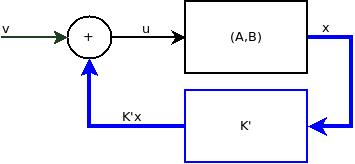
\includegraphics[scale=0.4]{./ControllabilityAfterFeedback.jpg}
 \caption{System $(\mathbf{A}+\mathbf{BK}',\mathbf{B})$ with input $v$} 
  \label{fig:controllabilityAfterFeedback}
\end{figure}
\begin{proposition}
 If $(\mathbf{A},\mathbf{B})$ is a controllable pair, then for every $\mathbf{K}\in M_{n\times m}(\mathbb{R})$ the pair $(\mathbf{A}+\mathbf{BK}',\mathbf{B})$ is also controllable.
\end{proposition}
\begin{proof}
 For the proof we employ the Hautus lemma. For $\lambda\in\mathbb{C}$ and $\mathbf{z}\in\mathbb{R}^{n+m}$ let us assume that:
\begin{equation}
 \mathbf{z}' \left[ {\begin{array}{cc} \lambda\mathbf{I}-(\mathbf{A}+\mathbf{BK}') & \mathbf{B} \end{array} } \right]=\mathbf{0}'
\end{equation}
Therefore
\begin{eqnarray}
 \mathbf{z}' \left( \lambda\mathbf{I}-(\mathbf{A}+\mathbf{BK}') \right) &=& \mathbf{0}'\\
 \mathbf{z}' \mathbf{B}  &=& \mathbf{0}'\label{eqn:zbis0}
\end{eqnarray}
From the first equation one has that:
\begin{eqnarray}
 \lambda\mathbf{z}'  -\mathbf{z}'\mathbf{A}-\mathbf{z}'\mathbf{BK}' = \mathbf{0}'
\end{eqnarray}
And due to (\ref{eqn:zbis0}) we have:
\begin{equation}
\left. {\begin{array}{c}
 \mathbf{z}'(\lambda\mathbf{I}  -\mathbf{A}) = \mathbf{0}'\\
 \mathbf{z}'\mathbf{B}=\mathbf{0}'
 \end{array} } \right\}
  \Rightarrow \mathbf{z}'  \left[ {\begin{array}{cc} \lambda\mathbf{I}-\mathbf{A} & \mathbf{B} \end{array} } \right]=\mathbf{0}'
\end{equation}
and again because of the Hautus lemma (and because the pair $(\mathbf{A},\mathbf{B})$ is controllable):
\begin{equation}
 \mathbf{z}=\mathbf{0}
\end{equation}
which completes the proof (read \hyperlink{note:hautusLemma}{the note} under lemma \ref{lemma:hautus})
\end{proof}



\subsection{Connection to the Diagonal Realization}
Earlier, in section \ref{sect:DiagonalRealization}, we referred to the connection between the diagonal realization of a system and its controllability. Consider of a system in the form (diagonalized and with the coefficients of the input vector normalized to 1):
\begin{equation}
 \frac{d}{dt}\left[ {\begin{array}{c}
 \zeta_1 \\
 \zeta_2 \\
 \vdots  \\
 \zeta_n
 \end{array} } \right] = 
\left[ {\begin{array}{cccc}
 \lambda_1 & & & \\
 & \lambda_2 & & \\
 & & \ddots & \\
 & & & \lambda_n
 \end{array} } \right]
\left[ {\begin{array}{c}
 \zeta_1 \\
 \zeta_2 \\
 \vdots  \\
 \zeta_n
 \end{array} } \right]+
\left[ {\begin{array}{c}
 1 \\
 1 \\
 \vdots  \\
 1
 \end{array} } \right]
 u(t)
\end{equation} 
Then, the controllability matrix of this system is:
\begin{equation}
 \mathcal{C} = \left[ {\begin{array}{ccccc}
 1 & \lambda_1 & \lambda_1^2 & \cdots & \lambda_1^n \\
 1 & \lambda_2 & \lambda_2^2 & \cdots & \lambda_2^n \\
 \vdots & \vdots &           & \ddots & \vdots \\
 1 & \lambda_n & \lambda_n^2 & \cdots & \lambda_n^n \\
 \end{array} } \right]
\end{equation}
Observe now that if two eigenvalues are equal, e.g. $\lambda_1=\lambda_2$, then $\mathcal{C}$ right away has two identical rows and its rank becomes less than $n$, therefore the system is not controllable. $\mathcal{C}$ possesses a very special form known as \emph{Van der Monde} matrix over the set of eigenvalues (Van der Monde matrices have numerous applications in numerical analysis and the Discreet Fourier Transform).

\begin{proposition}
Consider the system
\begin{equation}
 \dot{\mathbf{x}}=\mathbf{\Lambda x}+\mathbf{B}u
\end{equation}
 with $\mathbf{\Lambda}\in \mathfrak{dg}(n,\mathbb{R})$ and $\mathbf{B}\in M_{n\times 1}(\{0,1\})$, i.e. $\mathbf{\Lambda}$ is a diagonal matrix and the elements of $\mathbf{B}$ are either $0$ or $1$. This system is controllable if and only if $\mathbf{B}$ has no zero entries and $\mathbf{\Lambda}$ does not have repeated entries in its diagonal.
\end{proposition}

The above result can be extended to systems with many inputs. This way we state the following condition for controllability.
\begin{proposition}[Modal Controllability Criterion]
 Consider the LTI system with state equation $\dot{\mathbf{x}}=\mathbf{Ax}+\mathbf{Bu}$ where $\mathbf{A}$ is diagonalizable i.e. there is a $\mathbf{T}\in\text{GL}(n,\mathbb{R})$ so that $\mathbf{\Lambda}=\mathbf{TAT}^{-1}$ is diagonal. The diagonal form of the system is:
\begin{equation}
 \dot{\mathbf{x}}=\mathbf{\Lambda x}+\tilde{\mathbf{B}}\mathbf{u}
\end{equation}
where $\tilde{\mathbf{B}}=\mathbf{TB}$. If any of the rows of $\tilde{\mathbf{B}}$ is zero, then the system is not controllable.
\end{proposition}


\subsection{Controllability Gramian}
Until now we just now that if a system is controllable then for every pair of states $\mathbf{x}_1$ and $\mathbf{x}_2$, \emph{there exists} an input function $u(t)$ (depending on these states) so that it can steer the system's state from $\mathbf{x}_1$ (at $t=0$) to $\mathbf{x}_2$ at some desired finite time $t=T$. What we do not know yet is how to determine an input signal $\mathbf{u}(t)$ over $[0,T]$ so that $\mathbf{x}(0)=\mathbf{x}_1$ and $\mathbf{x}(T)=\varphi^{\mathbf{u}}(T;\mathbf{x}_1)=\mathbf{x}_2$. For that purpose, let us introduce the following function known as the \emph{Controllability Gramian} of the system:

\begin{definition}[Controllability Gramian]\hypertarget{def:contrGramian}
 For a pair of matrices $(\mathbf{A},\mathbf{B})$ that correspond to an \hyperlink{sec:LTI}{LTI} system, we define the Controllability Gramian of the system to be a mapping $W_c:\mathbb{R}\to M_n(\mathbb{R})$ with:
\begin{equation}\label{ContrlGram}
 W_c(t)\triangleq\int_0^t e^{\mathbf{A}(t-\tau)}\mathbf{BB}'e^{\mathbf{A}'(t-\tau)}d\tau
\end{equation}
\end{definition}
\noindent A simple change of coordinates $\xi(\tau)=t-\tau$, meaning $d\xi=-d\tau$, yields:
\begin{equation}
 W_c(t)=\int_{\xi(0)}^{\xi(t)} e^{\mathbf{A}\xi}\mathbf{BB}'e^{\mathbf{A}'\xi}(-d\xi)
=\int_0^t e^{\mathbf{A}\xi}\mathbf{BB}'e^{\mathbf{A}'\xi}d\xi
\end{equation}
The first thing to notice here is that $W_c$ is positive semidefinite (we denote $W_c(t)\succeq 0$ for all $t\in\mathbb{R}$), i.e. for every vector $\mathbf{z}$ it holds that:
\begin{equation}
 \mathbf{z}'W_c(t)\mathbf{z}\geq 0 \text{ for all } t\in\mathbb{R}
\end{equation}
Indeed, let $\mathbf{z}\in\mathbb{R}^n$. Then:
\begin{eqnarray}
 \mathbf{z}'W_c(t)\mathbf{z}
      &=&\int_0^t \mathbf{z}'e^{\mathbf{A}\tau}\mathbf{BB}'e^{\mathbf{A}'\tau}\mathbf{z}d\tau\\
      &=&\int_0^t \left(\mathbf{B}'e^{\mathbf{A}'\tau}\mathbf{z}\right)'\left(\mathbf{B}'e^{\mathbf{A}'\tau}\mathbf{z}\right)d\tau\\
      &=&\int_0^t \left\|\mathbf{B}'e^{\mathbf{A}'\tau}\mathbf{z} \right\|^2 d\tau \geq 0
\end{eqnarray}
\textbf{On Inner Product Spaces}: In order to understand what follows we need to meticulously make some remarks. So let $\mathcal{V}$ be an inner product space. A vector $\mathbf{y}$ is said to be perpendicular to $\mathbf{x}$ if $\langle\mathbf{y},\mathbf{x}\rangle=0$; we also denote $\mathbf{y}\perp\mathbf{x}$. Let $A\subseteq \mathcal{V}$; then we say that $\mathbf{y}$ is perpendicular to $A$ (we denote $\mathbf{y}\perp A$) if it is perpendicular to all vectors in $A$. If $A$ is a linear subspace of $\mathcal{V}$ and $\mathcal{B}_A$ is a basis for it then $\mathbf{y}$ is perpendicular to $A$ if it is perpendicular to all vectors in $\mathcal{B}_A$ ($\mathbf{y}\perp \mathcal{B}_A$). Finally, the only vector in $\mathcal{V}$ that is perpendicular to $\mathcal{V}$ is $\mathbf{0}$:
\begin{equation}
 \mathbf{x}\perp \mathcal{V} \Leftrightarrow \langle\mathbf{x},\mathbf{y} \rangle=0 \text{ for all } \mathbf{y}\in\mathcal{V} \Leftrightarrow \mathbf{x}=\mathbf{0}
\end{equation}
So for example in $\mathbb{R}^n$, recall that the inner product between two vectors is defined as 
\begin{equation}
 \langle\mathbf{x},\mathbf{y} \rangle\triangleq \mathbf{y}'\mathbf{x}
\end{equation}
Let $\{\mathbf{e}_i\}_{i=1}^n$ be a basis for $\mathbb{R}^n$ and $\mathbf{y}\in\mathbb{R}^n$ such that:
\begin{equation}
 \langle\mathbf{y},\mathbf{e}_i \rangle=0 \text{ for } i=1,2,\ldots,n
\end{equation}
Then, it follows that $\mathbf{y}=\mathbf{0}$. \\
\\
A more interesting example involves the vector space $\mathcal{L}^2([0,1])$ which is defined as follows:
\begin{equation}
 \mathcal{L}^2([0,1])\triangleq\left\{f:[0,1]\rightarrow\mathbb{R};\ \int_0^1 f^2(t)dt <\infty\right\}
\end{equation}
This is an inner product space and its inner product is defined as follows:
\begin{equation}
 \langle f,g \rangle \equiv\langle f,g \rangle_{\mathcal{L}^2([0,1])}\triangleq \int_0^1 f(t)g(t)dt
\end{equation}
So once again $f \perp \mathcal{L}^2([0,1])$ means that:
\begin{equation}
 \langle f,g \rangle =0 \text { for all } g \in \mathcal{L}^2([0,1])
\end{equation}
or equivalently
\begin{equation}
 \int_0^1 f(t)g(t)dt =0 \text { for all } g \in \mathcal{L}^2([0,1])
\end{equation}
which implies that $f=0$, i.e. $f(t)=0$ for all $t\in[0,1]$.
\begin{proposition}
 An LTI system is controllable if and only if its \hyperlink{def:contrGramian}{controllability gramian} is non-singular.
\end{proposition}
\begin{proof}
 1. Assume that the system is controllable. Then as we already know it is possible to steer the system from the origin $\mathbf{x}=\mathbf{0}$ to any desired state $\mathbf{x}^\star$ at some time instant $T$. Formally speaking, for every $T>0$ and for every $\mathbf{x}^\star\in\mathbb{R}^n$, there is an input signal $\mathbf{u}(\cdot)$ (defined over $[0,T]$) such that $\varphi^{\mathbf{u}}(T;\mathbf{0})=\mathbf{x}^\star$ or as we say ``$\varphi^{\mathbf{u}}(t;\mathbf{0})$ \emph{spans} the whole $\mathbb{R}^n$ - $\operatorname{span}_{t>0}\{\varphi^{\mathbf{u}}(t;\mathbf{0})\}=\mathbb{R}^n$''. (Recall that the only vector of $\mathbb{R}^n$ that is normal to all other vectors in the space is $\mathbf{0}$). Therefore, the following implication holds:
\begin{equation}\label{BHUI}
 \mathbf{z}\perp\varphi^{\mathbf{u}}(t;\mathbf{0}) \text{ for all }t\in[0,T] \text{ and for all }\mathbf{u}\in\mathcal{L}^2_{[0,T]} \implies \mathbf{z}=\mathbf{0}
\end{equation}
or what is the same:
\begin{equation}
 \mathbf{z}'\varphi^{\mathbf{u}}(T;\mathbf{0})=0  \text{ for all }\mathbf{u}\in\mathcal{L}^2_{[0,T]}\implies \mathbf{z}=\mathbf{0}
\end{equation}
The left-hand side of this equation can be rewritten as follows:
\begin{equation}
 \mathbf{z}'\int_0^T e^{\mathbf{A}(T-\tau)}\mathbf{Bu}(\tau)d\tau=0  \text{ for all }\mathbf{u}\in\mathcal{L}^2_{[0,T]}
\end{equation}
which implies that 
\begin{equation}
 \mathbf{z}'e^{\mathbf{A}(T-\tau)}\mathbf{B}=0 \text{ for all } \tau\in[0,T]
\end{equation}
From which we have that:
\begin{eqnarray}
 &&\int_0^t \mathbf{z}'e^{\mathbf{A}(t-\tau)}\mathbf{B}\left( \mathbf{z}'e^{\mathbf{A}(t-\tau)}\mathbf{B} \right)'=0\\
&\Leftrightarrow& \mathbf{z}'W_c(t)\mathbf{z}=0 \text{ for all }t\in[0,T]
\end{eqnarray}
Therefore (\ref{BHUI}) is rewritten as follows:
\begin{equation}
 \mathbf{z}'W_c(t)\mathbf{z}=0 \implies \mathbf{z}=\mathbf{0} \text{ for all } t>0
\end{equation}
And since we know that $W_c(t)$ is positive semidefinite for all $t>0$ we conclude that it is positive definite, i.e. for all $t>0$:
\begin{eqnarray}
 W_c(t) &\succeq& 0\\
 \mathbf{z}'W_c(t)\mathbf{z}&=&0 \implies \mathbf{z}=\mathbf{0}
\end{eqnarray}
Hence $W_c(t)$ is non-singular (positive definite matrices have only strictly positive eigenvalues and are non-singular).\\
\\
2. We will now assume that $W_c(t)$ is non-singular and we will prove that it is controllable. Let $\mathbf{x}_0$ and $\mathbf{x}_1$ be two distinct states in $\mathbb{R}^n$ and $T>0$. Then we will find an input signal $\mathbf{u}(t)$ (defined over $[0,T]$) so that $\varphi^{\mathbf{u}}(T;\mathbf{x}_0)=\mathbf{x}_1$ . Let:
\begin{equation}\label{STEER}
 \mathbf{u}(t)=\mathbf{B}'e^{(T-t)\mathbf{A}'}W_c(T)^{-1}\left[ \mathbf{x}_1-e^{T\mathbf{A}}\mathbf{x}_0\right]
\end{equation}
We then verify that:
\begin{eqnarray}
 \varphi^{\mathbf{u}}(T;\mathbf{x}_0) &=& e^{\mathbf{A}T} + \int_0^T e^{\mathbf{A}(T-\tau)}\mathbf{BB}'e^{(T-\tau)\mathbf{A}'}W_c(T)^{-1}\cdot\\ 
&& \cdot \left[ \mathbf{x}_1-e^{T\mathbf{A}}\mathbf{x}_0\right]d\tau\\
&=&e^{\mathbf{A}T} + \int_0^T e^{\mathbf{A}(T-\tau)}\mathbf{BB}'e^{(T-\tau)\mathbf{A}'}d\tau\\ 
&& \cdot W_c(T)^{-1}\left[ \mathbf{x}_1-e^{T\mathbf{A}}\mathbf{x}_0\right]\\
&=&e^{\mathbf{A}T} + W_c(T)W_c(T)^{-1}\left[ \mathbf{x}_1-e^{T\mathbf{A}}\mathbf{x}_0\right]\\
&=&  \mathbf{x}_1
\end{eqnarray}
which completes the proof
\end{proof}
\noindent Equation (\ref{STEER}) provides a way to move the state from any initial to any final point at some specified time instant. However this solution is \textbf{not unique} as there are lots of other ways to move from one state to another. In some cases constant or piecewise constant inputs (over $t$) are appropriate. Plausibly, one wonders how did such a complicated equation as (\ref{STEER}) occur. The answer will come up later as we study the Linear Quadratic Regulator.\\
\\
The Controllability Gramian is defined through (\ref{ContrlGram}) but when it comes to its calculation, we prefer to use the following proposition. The controllability gramian satisfies an Initial Value Problem (A differential equation and an Initial Condition). This is either solved analytically - if possible - or a numerical approximation method is chosen (e.g. Runge-Kutta).
\begin{proposition}
The controllability Gramian satisfies the following IVP:
\begin{eqnarray}
 \dot{W}_c &=& \mathbf{BB}'+\mathbf{A}W_c+W_c\mathbf{A}'\\
 W_c(0) &=& \mathbf{0}
\end{eqnarray}
\end{proposition}

\section{Controllability and Cyclicity}
In this section we give some results on controllability which will introduce us to the realm of its very algebraic nature. First we provide the definition of a cyclic space and a brief introduction to properties of cyclic spaces and in the sequel we try to savvy its connection to controllability:

\subsection{Introduction to cyclicity}
\begin{definition}[Cyclic subspace]
 Let $\mathbf{A}\in\mathbb{R}^n$ and $\mathbf{p}\in\mathbb{R}^n$. Let $\mathbb{R}[t]$ be the ring of polynomials over $\mathbb{R}$. We define the set:
 \begin{equation}
  \mathcal{Z}(\mathbf{A},\mathbf{p})\triangleq\{P(\mathbf{A})\mathbf{p};\ P\in\mathbb{R}[t]\}
 \end{equation}
 which is called an $\mathbf{A}$-cyclic subspace of $\mathbb{R}^n$ generated by $\mathbf{p}$. The vector $\mathbf{p}$ is called a generator of $\mathcal{Z}(\mathbf{A},\mathbf{p})$.
\end{definition}

\noindent \textbf{Note 1 :} $\mathcal{Z}(\mathbf{A},\mathbf{p})$ is an $\mathbf{A}$-\hyperlink{def:invariantSubspace}{invariant space}. Indeed, let $\mathbf{w}\in\mathcal{Z}(\mathbf{A},\mathbf{p})$. Then, there is a $P\in\mathbb{R}[t]$ so that $\mathbf{w}=P(\mathbf{A})\mathbf{p}$, therefore $\mathbf{Aw}=\mathbf{A}P(\mathbf{A})\mathbf{p}=Q(\mathbf{A})\mathbf{p}$ where $Q$ is another polynomial (in particular if $S(t)=t^2$ it is $Q=P\circ S$). Thus $\mathbf{Aw}\in\mathcal{Z}(\mathbf{A},\mathbf{p})$. Since $\mathcal{Z}(\mathbf{A},\mathbf{p})$ is $\mathbf{A}$-invariant, if $\mathbf{w}\in\mathcal{Z}(\mathbf{A},\mathbf{p})$ then $\mathbf{Aw},\mathbf{A}^2\mathbf{w},\ldots,\mathbf{A}^k\mathbf{w},\ldots\in\mathcal{Z}(\mathbf{A},\mathbf{p})$.\\
\\
\noindent \textbf{Note 2 :} $\mathcal{Z}(\mathbf{A},\mathbf{p})$ is the smallest $\mathbf{A}$-invariant subspace of $\mathbb{R}^n$ that contains $\mathbf{p}$. Formally:
\begin{equation}
 \mathcal{Z}(\mathbf{A},\mathbf{p}) = \bigcap \left\{ \mathcal{F}\hookrightarrow \mathbb{R}^n \ :\ \mathbf{A}\mathcal{F}\subseteq \mathcal{F},\ \mathbf{p}\in\mathcal{F}\right\}
\end{equation}
Indeed, it is easy to see that if $\mathcal{F}\hookrightarrow \mathbb{R}^n$ and $\mathcal{F}$ is $\mathbf{A}$-invariant with $\mathbf{p}\in\mathcal{F}$, then $\mathcal{Z}(\mathbf{A},\mathbf{p})\subseteq\mathcal{F}$. From the invariance property $\mathbf{A}^k\mathbf{p}\in\mathcal{F}$ for $k=0,1,\ldots$, thus for all $P\in\mathbb{R}[t]$ we have that $P(\mathbf{A})\mathbf{p}\in\mathcal{F}$.\\
\\
\noindent \textbf{Note 3 :} A polynomial of $\mathbb{R}[t]$ is made up as a finite linear combination of the elements:
\begin{equation}
 \mathbf{I},\mathbf{A},\mathbf{A}^2,\ldots,\mathbf{A}^k,\ldots
\end{equation}
i.e. for some positive integer $N$ it has the form:
\begin{equation}
 P(\mathbf{A})=a_0\mathbf{I}+a_1\mathbf{A}+\ldots+a_k\mathbf{A}^N=\sum_{i=0}^{N}a_i\mathbf{A}^i
\end{equation}
There is a minimum integer $k$ such that $\mathbf{A}^k$ is a linear combination of lower powers of $\mathbf{A}$:
\begin{equation}\label{eqn:Akspan}
 \mathbf{A}^k=\sum_{i=0}^{k-1} \gamma_i \mathbf{A}^i
\end{equation}
Right-multiplying by $\mathbf{p}$ yields:
\begin{equation}\label{eqn:AannihilatorOfp}
 \mathbf{A}^k\mathbf{p}=\sum_{i=0}^{k-1} \gamma_i \mathbf{A}^i\mathbf{p}
\end{equation}
This gives rise to the following important definition:
%
% A-annihilator of p
%
\begin{definition}[$\mathbf{A}$-annihilator of $\mathbf{p}$]\hypertarget{def:Aannihilator}
 An $\mathbf{A}$-annihilator of $\mathbf{p}$ \marginpar{A polynomial is called \textbf{monic} if its highest-order coefficient is 1.}is any monic \hypertarget{def:monic} polynomial  $\alpha\in\mathbb{R}[t]$ such that 
 \begin{equation}
  \alpha(\mathbf{A})\mathbf{p}=\mathbf{0}
 \end{equation} 
\end{definition}
%
% Existence of the A-annihilator
%
\noindent \textbf{Note} (Existence of $\mathbf{A}$-annihilators)\textbf{.} Given a vector $\mathbf{x}\in\mathbb{R}^n$ consider the sequence of vectors $\{\mathbf{x},\mathbf{Ax},\ldots\}$. We know that there is some $p\in\mathbb{N}$, $0\leq p \leq n$ so that $\mathbf{A}^p\mathbf{x}$ is a linear combination of $\mathbf{x},\mathbf{Ax},\ldots,\mathbf{A}^{p-1}\mathbf{x}$, that is:
\begin{equation}
 \mathbf{A}^p\mathbf{x}=\lambda_0\mathbf{x}+\lambda_1\mathbf{Ax}+\ldots+\lambda_{p-1}\mathbf{A}^{p-1}\mathbf{x}
\end{equation}
Let us define the polynomial $\pi\in\mathbb{R}[t]$ as:
\begin{equation}
 \pi(t)=t^p-\lambda_{p-1}t^{p-1}-\ldots-\lambda_1 t - \lambda_0
\end{equation}
It is easy to see that:
\begin{equation}
 \pi(\mathbf{A})\mathbf{x}=\mathbf{0}
\end{equation}
$\pi$ is an $\mathbf{A}$-annihilator of $\mathbf{x}$ according to the definition.
 
%
% MP of p
%
\begin{definition}[Minimum polynomial of a vector]\hypertarget{def:mpOfVector}
 The monic polynomial of the lowest degree that is an $\mathbf{A}$-annihilator of $\mathbf{p}$ is called the minimal polynomial of the vector $\mathbf{p}$ with respect to $\mathbf{A}$.
\end{definition}

\noindent \textbf{Note :} Following equation (\ref{eqn:AannihilatorOfp}), the $\mathbf{A}$-annihilator of $\mathbf{p}$ is given by:
\begin{equation}
 m(t)=t^k-\sum_{i=0}^{k-1} \gamma_i t^i
\end{equation}
The mp of a vector $\mathbf{p}$ (with respect to the matrix $\mathbf{A}$) is always a divider of the minimal polynomial of $\mathbf{A}$. We recall the definition of the minimal polynomial:
\begin{definition}[Minimal polynomial of a matrix]\hypertarget{def:minimalPolynomial}
 For a matrix $\mathbf{A}\in M_n(\mathbb{R})$ we define its minimal polynomial to be the \hyperlink{def:monic}{monic} polynomial $\mu\in\mathbb{R}[t]$ of minimum degree so that $\mu(\mathbf{A})=\mathbf{0}$.
\end{definition}
As it is known from Linear Algebra, the minimal polynomial of a matrix is uniquely defined and it always divides the characteristic polynomial of the matrix and it also divides any polynomial $q$ such that $q(\mathbf{A})=0$. With the following proposition we establish a relationship between the minimal polynomial of $\mathbf{A}$ and the minimal polynomials of the vectors of a basis of the whole space.
%
%
%
\begin{proposition}\label{prop:minimalPolynomialAndAnnihilators}
 Let $\mathbf{A}\in M_n(\mathbb{R})$ and $\mathcal{B}=\{\mathbf{b}_1,\mathbf{b}_2,\ldots,\mathbf{b}_n\}$ be a generator 
 \marginpar{The \textbf{least common multiple} (lcm) of two polynomials $\beta_1$ and $\beta_2$ is a polynomial $\xi$ such that $\beta_1|\xi,\ \beta_2|\xi$ and for $f\in\mathbb{R}[t]$ we have that $\beta_1|f,\beta_2|f\Rightarrow\xi|f$.}
of $\mathbb{R}^n$. Let $\beta_i\in\mathbb{R}[t]$ be the minimum polynomial of $\mathbf{b}_i$ with respect to $\mathbf{A}$. Then the minimal polynomial of $\mathbf{A}$ is the least common multiple (LCM) of $\beta_1,\beta_2,\ldots,\beta_n$:
 \begin{equation}
  \mu(t)=\operatorname{lcm}\{\beta_1,\beta_2,\ldots,\beta_n\}
 \end{equation}
\end{proposition}
\begin{proof}
 Let us define:
 \begin{equation}
  \beta(t)\triangleq\operatorname{lcm}\{\beta_1,\beta_2,\ldots,\beta_n\}
 \end{equation}
 \begin{claim}
  The minimum polynomial of $\mathbf{A}$ divides $\beta(t)$
 \end{claim}
 According to the definition of $\beta$, $\beta_i | \beta$ and $\beta_i(\mathbf{A})\mathbf{b}_i=\mathbf{0}$ for every $i$. Thus $\beta(\mathbf{A})\mathbf{b}_i=\mathbf{0}$ for each $i$, that is $\mathbf{b}_i\in\mathcal{N}(\beta(\mathbf{A}))$ for each $i$. Therefore, $\mathcal{B}\subseteq \mathcal{N}(\beta(\mathbf{A}))\Rightarrow\mathcal{N}(\beta(\mathbf{A}))=\mathbb{R}^n\Rightarrow\beta(\mathbf{A})=\mathbf{0}$. The minimum polynomial of $\mathbf{A}$ is known to divide all polynomials with the property $\beta(\mathbf{A})=\mathbf{0}$, hence $\mu|\beta$.
 \begin{claim}\label{claim:betaDividesMu}
  It also holds that $\beta|\mu$
 \end{claim}
 We perform the euclidean division of $\mu$ by $\beta$ and try to prove that the remainder must be 0. The degree of $\beta_i$ is less or equal that the degree of $\mu$, thus there exist polynomials $d_i$ and $r_i$ with $\operatorname{deg}r_i<\operatorname{deg}\beta_i$ such that:
 \begin{equation}
  \mu(t)=d_i(t)\beta_i(t)+r_i(t)
 \end{equation}
 We have that:
 \begin{equation}
  \mu(\mathbf{A})\mathbf{b}_i=d_i(\mathbf{A})\beta_i(\mathbf{A})\mathbf{b}_i+r_i(\mathbf{A})\mathbf{b}_i
 \end{equation}
 Notice that $\mu(\mathbf{A})\mathbf{b}_i=\mathbf{0}$ and $\beta_i(\mathbf{A})\mathbf{b}_i=\mathbf{0}$. Therefore $r_i(\mathbf{A})\mathbf{b}_i=\mathbf{0}$. This should mean that $r_i=0$; if not, then $r_i$ is a minimum polynomial of $\mathbf{b}_i$ (\textit{wrt} $\mathbf{A}$) with degree less than the degree of $\beta_i$ which is impossible according to the definition of the \hyperlink{def:mpOfVector}{minimum polynomial of a vector} (\textit{wrt} $\mathbf{A}$). Therefore $r_i$ is the zero polynomial.
\end{proof}
%
% A direct consequence
%
\noindent \textbf{Note :} It is a direct consequence of this proposition that if $\mathbf{x}\in\mathbb{R}^n$ is an arbitrary vector whose minimal polynomial with respect to $\mathbf{A}$ is $\chi\in\mathbb{R}[t]$ then $\chi|\mu$ (where $\mu$ is the minimal polynomial of the matrix $\mathbf{A}$).
%
% Description of Z(A,p)
%
\noindent To this end we can state and prove the following proposition:
\begin{proposition}[Description of $\mathcal{Z}(\mathbf{A},\mathbf{p})$]\label{prop:descriptionZAp}
 Let $k$ be the minimum positive integer such that $\mathbf{A}^k$ is in the span of $\mathbf{A}^i$ for $i=0,1,\ldots,k-1$ as in (\ref{eqn:Akspan}). The set $\mathcal{B}_{\mathcal{Z}}\triangleq\{\mathbf{p},\mathbf{Ap},\ldots,\mathbf{A}^{k-1}\mathbf{p}\}$ is a basis for $\mathcal{Z}(\mathbf{A},\mathbf{p})$.
\end{proposition}
\begin{proof}
 By definition of $k$ it holds that $\mathbf{A}^k\in\operatorname{span}\mathcal{B}_{\mathcal{Z}}$ and what is the same for every $s>k$ it also holds that $\mathbf{A}^s\in\operatorname{span}\mathcal{B}_{\mathcal{Z}}$. Therefore, for every $P\in\mathbb{R}[t]$ we have $P(\mathbf{A})\mathbf{p}\in\operatorname{span}\mathcal{B}_{\mathcal{Z}}$. It is left to the reader as an exercise to verify that $\mathcal{B}_{\mathcal{Z}}$ is linearly independent.
\end{proof}
%
% Definition of cyclic matrix
%
\begin{definition}[Cyclic matrix]\label{def:cyclicMatrix}\hypertarget{def:cyclicMatrix}
 A matrix $\mathbf{A}\in M_n(\mathbb{R})$ is called cyclic if there exists a $\mathbf{p}\in\mathbb{R}^n$ such that $\mathcal{Z}(\mathbf{A},\mathbf{p})=\mathbb{R}^n$. The vector $\mathbf{p}$ is called a generator of $\mathbb{R}^n$ with respect to $\mathbf{A}$.
\end{definition}
\noindent \textbf{Note :} According to this definition, a matrix $\mathbf{A}$ is cyclic if there exists a vector $\mathbf{p}\in\mathbb{R}^n$ such that:
\begin{equation}
 \operatorname{span}\left\{\mathbf{p},\mathbf{Ap},\ldots,\mathbf{A}^{n-1}\mathbf{p}\right\}=\mathbb{R}^n
\end{equation}

%
% Criterion for cyclicity
%
\begin{proposition}[Criterion for cyclicity]
 A matrix $\mathbf{A}$ is cyclic if and only if the degree of its minimal polynomial $\mu$ is $n$, i.e. if the minimal polynomial of $\mathbf{A}$ equals its characteristic polynomial.
\end{proposition}
\begin{proof}
 This is left to the reader as an exercise.
\end{proof}
%
% Remark:
\noindent \textbf{Remark :} A direct consequence of this proposition is that if a matrix has distinct (not repeated) eigenvalues then it is cyclic.\\
\\
\noindent The following proposition is some kind of converse to preposition \ref{prop:minimalPolynomialAndAnnihilators} and provides a sufficient condition for a vector to be a generator or $\mathbb{R}^n$ with respect to a cyclic matrix:
%
% π=μ => p is a generator
%
\begin{proposition}\label{prop:cyclicGeneratorMu=pi}
 Let $\mathbf{A}\in M_n(\mathbb{R})$ be a \hyperlink{def:cyclicMatrix}{cyclic matrix} and have \hyperlink{def:minimalPolynomial}{minimal polynomial} $\mu$. Let $\pi\in\mathbb{R}[t]$ be the minimum polynomial of $\mathbf{p}\in\mathbb{R}^n$ (\textit{wrt} $\mathbf{A}$). If $\pi=\mu$, then $\mathbf{p}$ is a generator of $\mathbb{R}^n$ with respect to $\mathbf{A}$. 
\end{proposition}
\begin{proof}
 Since $\mathbf{A}$ is cyclic, its minimal polynomial has degree $n$, i.e. has the form:
 \begin{equation}
  \mu(t)=t^n+\lambda_{n-1}t^{n-1}+\ldots+\lambda_1 t+\lambda_0
 \end{equation}
 for some reals $\lambda_0,\lambda_1,\ldots,\lambda_{n-1}$. We know that $\mu(\mathbf{A})\mathbf{p}=\mathbf{0}$ which is written as:
 \begin{equation}
  \mathbf{A}^n\mathbf{p}+\lambda_{n-1}\mathbf{A}^{n-1}\mathbf{p}+\ldots+\lambda_1 \mathbf{Ap}+\lambda_0\mathbf{p}=\mathbf{0}
 \end{equation}
 $\pi$ (i.e. $\mu$) is the monic polynomial of the smallest degree so that $\mu(\mathbf{A})\mathbf{p}=\mathbf{0}$. If $q\in\mathbb{R}[t]$ is of degree $<n$ then $q(\mathbf{A})\mathbf{p}\neq\mathbf{0}$. One can now verify that (this is an exercise) the set $\{\mathbf{p,\mathbf{Ap},\ldots,\mathbf{A}^{n-1}\mathbf{p}}\}$ is linearly independent thus generates $\mathbb{R}^n$ (Hint: Use the definition of a linearly independent set of vectors).
\end{proof}
%
% An important remark...
%
\noindent \textbf{An important remark:} Already from proposition \ref{prop:descriptionZAp} it has become clear that $\operatorname{deg }\pi=\operatorname{dim}\mathcal{Z}(\mathbf{A},p)$; the degree of the minimal polynomial of a vector is equal to the dimension of the cyclic subspace it generates. If it is supposed to generate the whole space $\mathbb{R}^n$ (with respect to $\mathbf{A}$), it is necessary that $\operatorname{deg}\pi=n$.

Before we state and prove a particularly important result related to cyclicity, we recall the definition of \emph{relatively prime} or \emph{coprime} polynomials:
\begin{definition}[Coprime polynomials]
 Let $p,q\in\mathbb{K}[t]$ 
 \marginpar{The \textbf{greatest common divider} of two polynomials $p$ and $q$ is a polynomial $d\in\mathbb{K}[t]$ such that $d|p,d|q$ and $s|p,s|q\Rightarrow s|d$}
 be two polynomials over a field $\mathbb{K}$ (e.g. $\mathbb{K}=\mathbb{R}$). 
 These are called relatively prime or comprime if there greatest common divider (gcd) is $1$.
\end{definition}
\noindent The following theorem is of high importance for coprime polynomials:
\begin{theorem}[GCD and Coprime polynomials]
 For any two polynomials $p,q\in\mathbb{K}[t]$ their greatest common divider is a linear combination of $p$ and $q$ with coefficients in $\mathbb{K}[t]$, i.e. there exist two polynomials $a,b\in\mathbb{K}[t]$ such that:
 \begin{equation}
  \operatorname{gcd}\{p(t),q(t)\}=a(t)p(t)+b(t)q(t)
 \end{equation}
 It is immediate that if $p$ and $q$ are coprime then there are polynomials $a,b\in\mathbb{K}[t]$ such that:
 \begin{equation}
  a(t)p(t)+b(t)q(t)=1
 \end{equation}
\end{theorem}
\begin{proof}
 A proof can be found in \cite[Thm. 1.16]{Kli+99}. More on coprime polynomials can be found in \cite[Chap. 4]{Bea96}.
\end{proof}
\noindent The following result is known as the Birkhoff-McLane lemma and is useful to establish a relationship between cyclicity and controllability in section \ref{sec:FromCyclicityToControllability}. The proof is extracted from \cite{Won67}:
\begin{lemma}[Birkhoff-McLane]\hypertarget{lemma:birkhoffMcLane}
 Let $\mathbf{A}$ be a \hyperlink{def:cyclicMatrix}{cyclic matrix} with \hyperlink{def:minimalPolynomial}{minimal polynomial} $\mu$. Let $\mathbf{b}$ be a generator of $\mathbb{R}^n$ with respect to $\mathbf{A}$ (i.e. $\mathcal{Z}(\mathbf{A},\mathbf{b})=\mathbb{R}^n$). Let $\gamma\in\mathbb{R}[t]$ be a polynomial that is relatively prime with $\mu$. Then the vector $\mathbf{p}=\gamma(\mathbf{A})\mathbf{b}$ is a generator of $\mathbb{R}^n$ with respect to $\mathbf{A}$.
\end{lemma}
\begin{proof}
 The proof goes along the lines of proof of proposition \ref{prop:minimalPolynomialAndAnnihilators}. Let first of all $\pi\in\mathbb{R}[t]$ be the minimum polynomial of $\mathbf{p}$, i.e. $\pi(\mathbf{A})\mathbf{p}=\mathbf{0}$. According to proposition \ref{prop:cyclicGeneratorMu=pi}, it suffices to show that $\pi=\mu$; We first prove that $\mu|\pi$ and then that $\pi|\mu$. Since $\gamma$ and $\mu$ are coprime, there are polynomials $\rho,\sigma\in\mathbb{R}[t]$ such that for all $t\in\mathbb{R}$:
 \begin{eqnarray}
  &&\rho(t)\gamma(t)+\sigma(t)\mu(t) = 1  \\
  &\Leftrightarrow&\rho(\mathbf{A})\gamma(\mathbf{A})+\sigma(\mathbf{A})\mu(\mathbf{A}) = \mathbf{I}  \\
&\Leftrightarrow&\rho(\mathbf{A})\gamma(\mathbf{A})\mathbf{b}+\sigma(\mathbf{A})\mu(\mathbf{A})\mathbf{b} = \mathbf{b}  \\
&\Leftrightarrow&\rho(\mathbf{A})\mathbf{p} = \mathbf{b} 
 \end{eqnarray}
Let $\mathbf{x}\in\mathbb{R}^n=\mathcal{Z}(\mathbf{A},\mathbf{b})$ be an arbitrary vector. Then, there exists a polynomial $\vartheta\in\mathbb{R}[t]$ such that:
\begin{equation}
 \mathbf{x}=\vartheta(\mathbf{A})\mathbf{b}=\vartheta(\mathbf{A})\rho(\mathbf{A})\mathbf{p}
\end{equation}
Hence
\begin{equation}\label{eqn:113243}
 \pi(\mathbf{A})\mathbf{x}=\pi(\mathbf{A})\vartheta(\mathbf{A})\rho(\mathbf{A})\mathbf{p}=\mathbf{0}
\end{equation}
This implies that $\pi(\mathbf{A})=0$. Indeed, (\ref{eqn:113243}) tells us that $\mathbf{x}\in\mathcal{N}(\pi(\mathbf{A}))$ for all $\mathbf{x}\in\mathbb{R}^n$, thus $\mathcal{N}(\pi(\mathbf{A}))=\mathbb{R}^n$ or what is the same $\pi(\mathbf{A})=\mathbf{0}$. Since $\pi(\mathbf{A})=0$ it follows immediately that $\mu|\pi$. From claim \ref{claim:betaDividesMu} within the proof of proposition \ref{prop:minimalPolynomialAndAnnihilators} it follows that $\pi|\mu$. Overall $\pi=\mu$ and according to proposition \ref{prop:cyclicGeneratorMu=pi} $\mathbf{p}$ is a generator of $\mathbb{R}^n$ with respect to $\mathbf{A}$.
\end{proof}


\subsection{From cyclicity to controllability}\label{sec:FromCyclicityToControllability}
The notion of cyclicity allows us to make a connection with the one of controllability. It is straightforward to notice that $\mathbf{A}$ is \hyperlink{def:cyclicMatrix}{cyclic} with generator $\mathbf{p}$ if and only if $(\mathbf{A},\mathbf{p})$ is controllable. Another simple result is stated as follows:
\begin{proposition}
 Let $\mathbf{A}\in M_{n}(\mathbb{R})$ and $\mathbf{b}\in\mathbb{R}^n$. The following are equivalent:
 \begin{enumerate}
  \item $(\mathbf{A},\mathbf{b})$ is controllable and $\mathbf{A}$ is cyclic.
  \item The set $\mathcal{B}\triangleq\{\mathbf{b},\mathbf{Ab},\ldots,\mathbf{A}^{n-1}\mathbf{b}\}$ is linearly independent.
 \end{enumerate}
\end{proposition}
\begin{proof}
 The proof is simple and is left to the reader as an exercise.
\end{proof}
Now we will state the main result of this section which is due to W.M. Wonham \cite{Won67}. It is often the case that none of the inputs to a system can guarantee controllability although the overall system is controllable. For instance, consider the system with 2 states and 2 inputs:
 \begin{eqnarray}
\dot{\mathbf{x}}(t)&=&\left[ {\begin{array}{cc}
 1 & 1  \\
 2 & 1  \\
 \end{array} } \right]
\mathbf{x}(t)+ 
\left[ {\begin{array}{cc}
 \frac{1}{\sqrt{2}}  & 1\\
 1 & -\sqrt{2}\\
 \end{array} } \right]
\mathbf{u}(t)
\end{eqnarray}
This system has controllability matrix:
\begin{equation}
 \mathcal{C}=\left[ {\begin{array}{cccc}
 \frac{1}{\sqrt{2}} & 1 & 1+\frac{1}{\sqrt{2}} & 1-\sqrt{2}\\
 1 & -\sqrt{2} & 1+\sqrt{2} & 2-\sqrt{2}
 \end{array} } \right]
\end{equation}
which is full-rank and the system is controllable. If we eliminate the second input we come up with the single input system:
 \begin{eqnarray}
\dot{\mathbf{x}}(t)&=&\left[ {\begin{array}{cc}
 1 & 1  \\
 2 & 1  \\
 \end{array} } \right]
\mathbf{x}(t)+ 
\left[ {\begin{array}{c}
 \frac{1}{\sqrt{2}}\\
 1
 \end{array} } \right]
u_1(t)
\end{eqnarray}
this system is not controllable. The same exactly will happen if we eliminate the first input. The system becomes:
 \begin{eqnarray}
\dot{\mathbf{x}}(t)&=&\left[ {\begin{array}{cc}
 1 & 1  \\
 2 & 1  \\
 \end{array} } \right]
\mathbf{x}(t)+ 
\left[ {\begin{array}{c}
  1\\
 -\sqrt{2}
 \end{array} } \right]
u_2(t)
\end{eqnarray}
which is again not controllable. We understand that \textbf{we need} both inputs to completely control the system.
A question that comes up is whether there is \emph{any} other input that leads to a controllable system. The answer is
positive if $\mathbf{A}$ is cyclic (see theorem \ref{thm:wonham}). In this example you can see that if we change the input into $v(t)=u_1(t)+u_2(t)$, or in matrix-vector form:
\begin{equation}
 v(t)=\left[ {\begin{array}{cc}1&1\end{array} } \right]\mathbf{u}(t)
\end{equation}
The new system with input $v(t)$ will be:
 \begin{eqnarray}
\dot{\mathbf{x}}(t)&=&\left[ {\begin{array}{cc}
 1 & 1  \\
 2 & 1  \\
 \end{array} } \right]
\mathbf{x}(t)+ 
\left[ {\begin{array}{c}
  1+\frac{1}{\sqrt{2}}\\
 1-\sqrt{2}
 \end{array} } \right]
v(t)
\end{eqnarray}
which is controllable by means of a single input.
%
%
% Wonham's theorem
%
\begin{theorem}[Wonham's theorem]\label{thm:wonham}
 Let $\mathbf{A}\in M_n(\mathbb{R})$ and $\mathbf{B}\in M_{n\times m}(\mathbb{R})$. \marginpar{$\mathcal{R}(\mathbf{B})$ denotes the image/column-space of the matrix $\mathbf{B}$} If $(\mathbf{A},\mathbf{B})$ is controllable and $\mathbf{A}$ is cyclic then there is a $\mathbf{b}\in\mathcal{R}(\mathbf{B})$ so that $(\mathbf{A},\mathbf{b})$ is controllable.
\end{theorem}
%
% Proof to Wonham's theorem
%
\begin{proof}
 Finding a $\mathbf{b}\in\mathcal{R}(\mathbf{B})$ such that $(\mathbf{A},\mathbf{b})$ is controllable is equivalent to determining such a vector so that it is a generator of $\mathbb{R}^n$ with respect to $\mathbf{A}$ (see definition \ref{def:cyclicMatrix}). For this reason we shall use the \hyperlink{lemma:birkhoffMcLane}{Birkhoff-McLane lemma}.

Let $\mathbf{b}_i\in\mathbb{R}^n$ be the i-th column-vector of $\mathbf{B}$ and $\beta_i$ its minimal polynomial with respect to $\mathbf{A}$. Let $\mu$ be the minimal polynomial of $\mathbf{A}$. According to proposition \ref{prop:minimalPolynomialAndAnnihilators} it is:
 \begin{equation}
  \mu=\operatorname{lcm}\left\{\beta_1,\beta_2,\ldots,\beta_m\right\}
 \end{equation}
 Let $\mathbf{z}\in\mathbb{R}^n$ be a generator of $\mathbb{R}^n$ with respect to $\mathbf{A}$. For each $i=1,2,\ldots,m$ there is a $\gamma_i\in\mathbb{R}[t]$ so that $\mathbf{b}_i=\gamma_i(\mathbf{A})\mathbf{z}$. We need to determine numbers $r_1,r_2,\ldots,r_m$ so that the vector $\tilde{\mathbf{b}}=r_1\mathbf{b}_1+r_2\mathbf{b}_2+\ldots+r_m\mathbf{b}_m$ is a generator of $\mathbb{R}^n$ \textit{wrt} $\mathbf{A}$. According to the Birkhoff-McLane lemma, it suffices to choose $r_i$ so that the polynomial:
 \begin{equation}
  \gamma(t)=r_1\gamma_1(t)+r_2\gamma_2(t)+\ldots+r_m\gamma_m(t)
 \end{equation}
 is coprime with $\mu$. The roots of $\mu$ are the eigenvalues of $\mathbf{A}$ in $\mathbb{C}$. In order for $\mu$ and $\gamma$ to be coprime we require that $\gamma(\lambda_j)\neq 0$ for all $\lambda_j\in\sigma(\mathbf{A})$.
 \begin{claim} The polynomials $\mu,\gamma_1,\gamma_2,\ldots,\gamma_m$ are coprime:
  \begin{equation}\label{eqn:claim3}
   \operatorname{gcd}\{\mu,\gamma_1,\gamma_2,\ldots,\gamma_m\}=1
  \end{equation}
 \end{claim}
 \begin{proof}[Proof of the claim]
  Let $\kappa=\operatorname{gcd}\{\mu,\gamma_1,\gamma_2,\ldots,\gamma_m\}$. By definition of the GCD, $\kappa|\mu$, thus there is a polynomial $\hat{\mu}$ so that 
 $\mu=\kappa\hat{\mu}$. Similarly, for every $i=1,2,\ldots,m$ we have that $\kappa|\gamma_i$, hence there exist polynomials $\hat{\gamma}_i$ such that $\gamma_i=\kappa\hat{\gamma}_i$. Then:
 \begin{eqnarray}
  \hat{\mu}(\mathbf{A})\mathbf{b}_i&=&\hat{\mu}(\mathbf{A})\gamma_i(\mathbf{A})\mathbf{z}\\
&=&\hat{\mu}(\mathbf{A})\kappa(\mathbf{A})\hat{\gamma}_i(\mathbf{A})\mathbf{z}\\
&=&\mu(\mathbf{A})\hat{\gamma}_i(\mathbf{A})\mathbf{z}\\
&=&\mathbf{0}
 \end{eqnarray}
This means that $\hat{\mu}$ is an $\mathbf{A}$-annihilator of $\mathbf{b}_i$, hence the minimal polynomial of $\mathbf{b}_i$, namely $\beta_i$, divides $\hat{\mu}$:
\begin{eqnarray}
&& \beta_i|\hat{\mu} \text{ for all }i=1,2,\ldots,m\\
&\Rightarrow& \operatorname{lcm}\{\beta_i\}_{i=1}^m|\hat{\mu}\\
&\Rightarrow& \mu|\hat{\mu}
\end{eqnarray}
It is obvious that $\hat{\mu}|\mu$ (indeed, $\mu=\kappa\hat{\mu}$). Therefore $\mu|\hat{\mu},\hat{\mu}|\mu\Rightarrow \mu=\hat{\mu}$ which implies that $\kappa=1$. The proof of the claim is complete.
 \end{proof}
By equation (\ref{eqn:claim3}) and by the fact that for each eigenvalue $\lambda_j$ of $\mathbf{A}$ it is $\mu(\lambda_j)=0$ it is not possible that $\gamma_i(\lambda_j)=0$ simultaneously for all $i=1,2,\ldots,m$.
\end{proof}

%
%
%
%\chapter{Observability and State Observer Design}
%
%
%
%
\chapter{Stability}
\section{Definitions}
In this section we give the basic definitions regarding \emph{stability} of state space systems. Readers might be already familiar with the kind of stability known as \emph{BIBO (bounded-input bounded-output) stability} and various criteria based on the \emph{transfer function} of the system such as the \emph{Routh criterion} or the \emph{Nyquist} one. Here we tackle the notion of stability considering always the closed-loop form of the system instead of an input-output formulation. From this point of view, any state space system of the form:
\begin{equation}
 \dot{\mathbf{x}}=f(\mathbf{x},\mathbf{u})
\end{equation}
using a feedback law $\mathbf{u}=\rho(\mathbf{x})$ becomes
\begin{equation}
 \dot{\mathbf{x}}=f(\mathbf{x},\rho(\mathbf{x}))=h(\mathbf{x})
\end{equation}
In what follows we always assume that $h:\mathbb{R}^n\to\mathbb{R}^n$ is Lipschitz, that is there exists a constant $L\geq 0$ so that for every $\mathbf{x},\mathbf{y}\in\mathbb{R}^n$:
\begin{equation}
 \|h(\mathbf{x})-h(\mathbf{y})\|\leq L\|\mathbf{x}-\mathbf{y}\|
\end{equation}
So, our analysis here takes into account the closed loop form of the system. The feedback law $\rho$ will be properly chosen so that the closed loop system exhibits the desired dynamic characteristics. For consistency we recall the definition of an equilibrium point:
\begin{definition}
 Consider the following autonomous state space system in closed-loop form:
\begin{equation}
 \dot{\mathbf{x}}=h(\mathbf{x})\label{PJ8}
\end{equation}
A point $\mathbf{x}^\star\in\mathbb{R}^n$ is said to be an equilibrium point for (\ref{PJ8}) if $h(\mathbf{x}^\star)=\mathbf{0}$.
\end{definition}
If $h$ is linear, i.e. $h(\mathbf{x})=\mathbf{Ax}$ then an equilibrium point for $f$ has the property:
\begin{equation}
 \mathbf{Ax}^\star=\mathbf{0}\Leftrightarrow\mathbf{x}\in\operatorname{ker}\mathbf{A}
\end{equation}
Where $\operatorname{ker}\mathbf{A}$ is the \emph{kernel} of the matrix $\mathbf{A}$, defined as:
\begin{equation}
 \operatorname{ker}\mathbf{A}\triangleq\{\mathbf{y}\in\mathbb{R}^n|\mathbf{Ay}=\mathbf{0}\}
\end{equation}
If $\mathbf{A}$ is invertible then $\operatorname{ker}\mathbf{A}$ is a singleton $\operatorname{ker}\mathbf{A}=\{\mathbf{0}\}$. In general, $\operatorname{ker}\mathbf{A}$ is a linear subspace of $\mathbb{R}^n$ with dimension $\operatorname{dim}(\operatorname{ker}\mathbf{A})=n-\operatorname{rank}\mathbf{A}$ (as it follows from the \emph{dimension theorem} of Linear Algebra).

\begin{example}
 The following LTI system is given:
\begin{eqnarray}
 \dot{\mathbf{x}}(t)&=&\left[ {\begin{array}{ccc}
 1 & 2 & -1 \\
 2 & 4 & 3  \\
 1 & 2 & 1
 \end{array} } \right]
\mathbf{x}(t)\label{XLTI101}
\end{eqnarray}
We need to determine all its equilibrium points. So, let $\mathbf{x}^\star=[x_1^\star \ \  x_2^\star \ \  x_3^\star]'$ be an equilibrium point for this system. Then:
\begin{eqnarray}
 \left[ {\begin{array}{ccc}
 1 & 2 & -1 \\
 2 & 4 & 3  \\
 1 & 2 & 1
 \end{array} } \right]\left[ {\begin{array}{c}
 x_1^\star \\
 x_2^\star  \\
 x_3^\star
 \end{array} } \right]=\mathbf{0}\Leftrightarrow
\left\{ {\begin{array}{c}
 x_1^\star+2x_2^\star-x_3^\star=0 \\
 2x_1^\star+4x_2^\star+3x_3^\star=0 \\
 x_1^\star+2x_2^\star+x_3^\star=0 
 \end{array} } \right.
\end{eqnarray}
Subtracting the third from the first row yields:
\begin{equation}
x_3^\star=0 
\end{equation}
And by means of the second-row equation we have that
\begin{equation}
 2x_1^\star+4x_2^\star=0\Leftrightarrow x_1^\star=-2x_2^\star
\end{equation}
So if $x_1^\star=\lambda$ then $x_2^\star=-\lambda/2$.
Hence any equilibrium point of (\ref{XLTI101}) has the form:
\begin{equation}
 \mathbf{x}^\star=\left[ {\begin{array}{c}
 \lambda \\
 -\lambda/2  \\
 0
 \end{array} } \right]=\lambda\left[ {\begin{array}{c}
 1 \\
 -1/2  \\
 0
 \end{array} } \right]
\end{equation}
The set of all equilibrium point for $\lambda\in\mathbb{R}$ forms a linear subspace of $\mathbb{R}^3$ of dimension 1 (i.e. the set of equilibrium points is a line in the 3-dimensional space).
\end{example}

If $\mathbf{x}^\star$ is an equilibrium point for (\ref{PJ8}) and $\varphi(t;\mathbf{x}^\star)$ the solution with $\varphi(0;\mathbf{x}^\star)=\mathbf{x}^\star$ then for all $t\geq 0$ we also have $\varphi(t;\mathbf{x}^\star)=\mathbf{x}^\star$, that is every solution starting for an equilibrium point will remain on that. But what happens is we start from a point $\mathbf{x}_0$ that is $\varepsilon$-close to that equilibrium point; for linear systems the following three options are possible:
\begin{enumerate}
 \item The equilibrium point will attract the initial point and eventually the trajectory will converge to it, in the sense that $\lim_{t\to\infty}\varphi(t;\mathbf{x}_0)=\mathbf{x}^\star$
 \item The equilibrium point will repulse the initial point and the state trajectory will move to infinity $\lim_{t\to\infty}\|\varphi(t;\mathbf{x}_0)\|=\infty$
 \item The trajectory will retain a constant distance from the equilibrium point
\end{enumerate}
These are incorporated into the definition of stability which is stated as follows for nonlinear systems:
\begin{definition}\label{stability-definition}\hypertarget{stability-definition}
 Consider a system in the form (\ref{PJ8}) and let $\mathbf{x}^\star$ be an equilibrium point for it. This point is called a stable equilibrium point if for every $\varepsilon>0$ there is a $\delta(\varepsilon)>0$ so that $\|\mathbf{x}-\mathbf{x}^\star\|<\delta\implies\|\varphi(t;\mathbf{x})\|<\varepsilon$ for all $t\geq 0$.
\end{definition}
According to this definition, for every ball $\mathcal{B}_\varepsilon(\mathbf{x}^\star)$ around the equilibrium point $\mathbf{x}^\star$, we can find some other ball $\mathcal{B}_\delta(\mathbf{x}^\star)$ so that starting from therein, the whole trajectory remains in $\mathcal{B}_\varepsilon(\mathbf{x}^\star)$. It is implied in the definition that $\delta\leq \varepsilon$ and \emph{a fortiori} $\mathcal{B}_\delta(\mathbf{x}^\star)\subseteq\mathcal{B}_\varepsilon(\mathbf{x}^\star)$. However, if a trajectory retains a constant distance from an  equilibrium point (e.g. the trajectory is a circle with center $\mathbf{x}^\star$ and radius $\delta$), then it is again a locally stable equilibrium point. It is clear that stability, as it is given in definition \ref{stability-definition} does not suggest that the trajectory converges to the equilibrium point. For that reason we introduce the notion of a locally \emph{asymptotically} stable point.
\begin{definition}[Local Asymptotic Stability]\label{definition:LAS}\hypertarget{definition:LAS}
 Consider a system in the form (\ref{PJ8}) and let $\mathbf{x}^\star$ be an equilibrium point for it. This point is called a locally asymptotically stable (LAS) equilibrium point if it is a stable equilibrium point and there is a $\delta>0$ such that $\lim_{t\to\infty}\varphi(t;\mathbf{x})=\mathbf{x}^\star$ for all $\mathbf{x}$ with $\|\mathbf{x}-\mathbf{x}^\star\|<\delta$.
\end{definition}
\emph{Remark :} The limit in this definition is meant in the norm sense, that is:
\begin{equation}
 \lim_{t\to\infty}\varphi(t;\mathbf{x})=\mathbf{x}^\star\Leftrightarrow\lim_{t\to\infty}\|\varphi(t;\mathbf{x})-\mathbf{x}^\star\|=0
\end{equation}
If in definition \ref{definition:LAS}, we change $\delta$ into $\infty$ we then come up with the definition of \emph{global} asymptotic stability which is given as follows:
\begin{definition}
 Consider a system in the form (\ref{PJ8}) and let $\mathbf{x}^\star$ be an equilibrium point for it. This point is called a globally asymptotically stable equilibrium point if it is a stable equilibrium point and $\lim_{t\to\infty}\varphi(t;\mathbf{x})=\mathbf{x}^\star$ for all $\mathbf{x}\in\mathbb{R}^n$.
\end{definition}
For a locally asymptotically stable point $\mathbf{x}^\star$ we define its \emph{domain of attraction} to be the set of all initial points that will eventually converge to it:
\begin{definition}
 Consider a system in the form (\ref{PJ8}) and let $\mathbf{x}^\star$ be a locally asymptotically stable equilibrium point. The following set is called the domain of attraction of $\mathbf{x}^\star$.
\begin{equation}
 \mathcal{S}(\mathbf{x}^\star)=\left\{\mathbf{x}\in\mathbb{R}^n | \lim_{t\to\infty}\varphi(t;\mathbf{x})= \mathbf{x}^\star\right\}\label{DoA}
\end{equation}
\end{definition}
It is obvious that in any case, if  $\mathbf{x}^\star$ is a locally asymptotically stable point then  $\mathbf{x}^\star\in\mathcal{S}( \mathbf{x}^\star)$. Additionally  $\mathbf{x}^\star$ is globally asymptotically stable if and only if $\mathcal{S}(\mathbf{x}^\star)=\mathbb{R}^n$.

Asymptotic stability can be understood using the so-called $\mathcal{KL}$-functions. We give the following definitions:
\begin{definition}\hypertarget{K-class}
We define the following four classes of functions:
\begin{enumerate}
 \item A function $\alpha:\mathbb{R}^+\to\mathbb{R}^+$ is said to be $\mathcal{K}$-class and we denote $\alpha\in\mathcal{K}$ if it is continuous, strictly increasing and $\alpha(0)=0$.
\item A function $\beta:\mathbb{R}^+\to\mathbb{R}^+$ is said to be $\mathcal{K}_\infty$-class and we denote $\beta\in\mathcal{K}_\infty$ if $\beta\in\mathcal{K}$ and it is unbounded.
\item A $\mu:\mathbb{R}^+\to\mathbb{R}^+$ is said to be $\mathcal{L}$-class and we denote $\mu\in\mathcal{L}$ if it is continuous, strictly decreasing and $\lim_{\tau\to\infty}\mu(\tau)=0$.
\item A $\gamma:\mathbb{R}^+\times\mathbb{R}^+\to\mathbb{R}^+$ is said to be $\mathcal{KL}$-class and we denote $\gamma\in\mathcal{KL}$ if $\gamma(\cdot,t)\in\mathcal{K}$ for all $t\in\mathbb{R}^+$ and $\gamma(r,\cdot)\in\mathcal{L}$ for all $r\in\mathbb{R}^+$.
\end{enumerate}
\end{definition}

\section{Some preliminary results}
In this section we state some results that hold for nonlinear systems in general. 
We start with the following characterization of stability:
%
% STABILITY in terms of K-class FUNCTIONS
%
%
\begin{proposition}[Characterization of Stability]\label{K-class-stable}
 The equilibrium point $\mathbf x^\star$ is \hyperlink{stability-definition}{stable} for the system (\ref{PJ8}) if and only if
there is a \hyperlink{K-class}{$\mathcal K$-class} function $\alpha(\cdot)$ and a constant $c>0$ such that:
\begin{equation}\label{FMLKASFER23}
 \|\varphi(t,\mathbf x_0)-\mathbf x^\star\|\leq \alpha(\|\mathbf x_0-\mathbf x^\star\|)
\end{equation}
For all $t\geq 0$ and for all $\mathbf x_0$ such that $\|\mathbf x_0-\mathbf x^\star\|<c$.
\end{proposition}
\begin{proof}
In what follows we adopt the notation $\mathcal{B}_{\varepsilon}(\mathbf{x}^\star)=\left\{
\mathbf{x}\in\mathbb{R}^n,\ \|\mathbf{x}-\mathbf{x}^\star\|<\varepsilon
\right\}$.
%
%
 $\Leftarrow.$ First suppose there is a $\mathcal{K}$-class function $\alpha$
and a positive constant $c$ such that (\ref{FMLKASFER23}) holds for all 
$t\geq 0$ and for all $\mathbf x_0\in\mathcal{B}_{\varepsilon}(\mathbf{x}^\star)$.
Let $\varepsilon>0$. Define $\delta(\varepsilon)\triangleq\min\{c,\alpha^{-1}(\varepsilon)\}$
and notice that $\delta<\alpha^{-1}(\varepsilon)$
Then, $\mathbf{x}_0\in\mathcal{B}_{\delta}(\mathbf{x}^\star)$ implies that
\begin{equation}\label{QLS3PA7}
 \|\varphi(t,\mathbf{x}_0)-\mathbf{x}^\star\|\leq
\alpha\left(\left\| \mathbf{x}_0-\mathbf{x}^\star \right\|\right)
< \alpha(\delta)\leq \alpha(\alpha^{-1}(\varepsilon))=\varepsilon
\end{equation}
At the second step we used the fact that $\left\| \mathbf{x}_0-\mathbf{x}^\star \right\|<\delta$.
Equation (\ref{QLS3PA7}) suggests that $\mathbf{x}^\star$ is stable.\\
\\
$\Rightarrow.$ Suppose that given $\varepsilon>0$, there is a $\delta=\delta(\varepsilon)>0$
such that 
\begin{equation}\label{9243123}
 \|\mathbf{x}_0-\mathbf{x}^\star\|<\delta(\varepsilon) \Rightarrow \|\varphi(t,\mathbf{x}_0)-\mathbf{x}^\star\|<\varepsilon
\end{equation}
for all $t\geq 0$. 
Actually, we are looking for a function $\delta(\varepsilon)$ that is $\mathcal{K}$-class that 
satisfies (\ref{9243123}).
Let $\bar{\delta}(\varepsilon)$ be the supremum over all functions such that (\ref{9243123})
holds. $\bar{\delta}$ is obviously positive and nondecreasing but needs not be continuous.
We may find $k\in(0,1)$ such that $\zeta(\varepsilon)<k\bar{\delta}(\varepsilon)$ with $\zeta\in\mathcal K$.
This way we rewrite (\ref{9243123}) replacing the arbitrary function $\delta$ by the $\mathcal K$-class
function $\zeta$.
\begin{equation}
 \|\mathbf{x}_0-\mathbf{x}^\star\|<\zeta(\varepsilon) \Rightarrow \|\varphi(t,\mathbf{x}_0)-\mathbf{x}^\star\|<\varepsilon
\end{equation}
The function we were looking for is finally $\alpha(\varepsilon)\triangleq\zeta^{-1}(\varepsilon)$. Define
$c=\lim_{r\to\infty}\zeta(r)$; If $r<c$ then $\alpha(r)<\infty$. Let $\mathbf{x}_0$ be given so that
$\|\mathbf{x}_0-\mathbf{x}^\star\|<c$ and let $\varepsilon=\alpha(\|\mathbf{x}_0-\mathbf{x}^\star\|)$.
Then, $\|\mathbf{x}_0-\mathbf{x}^\star\|<\bar{\delta}(\varepsilon)$, hence by (\ref{9243123}),
\begin{equation}
 \|\varphi(t,\mathbf{x}_0)-\mathbf{x}^\star\|<\varepsilon=\alpha(\|\mathbf{x}_0-\mathbf{x}^\star\|)
\end{equation}
and this completes the proof.
\end{proof}
%
%
%
%
% Characterization of ASYMPTOTICALLY STABLE POINTS
% via KL-class FUNCTIONS
%
In the following proposition we use the notion of $\mathcal{KL}$-class functions 
as defined above to state a very useful result on asymptotic stability.
\begin{proposition}\label{LASdefEquiv}
 Consider a system in the form (\ref{PJ8}) and let $\mathbf{x}^\star$ be an equilibrium
 point for it. The point is \hyperlink{definition:LAS}{locally asymptotically stable} if and only if there is a 
 \hyperlink{K-class}{$\gamma\in\mathcal{KL}$} and a constant $\kappa>0$ so that:
\begin{equation}
 \|\varphi(t;\mathbf{x}_0)-\mathbf{x}^\star\|\leq \gamma(\|\mathbf{x}_0-\mathbf{x}_\star\|,t)\label{KLPROP}
\end{equation}
for all $\mathbf{x}_0$ such that $\|\mathbf{x}_0-\mathbf{x}^\star\|<\kappa$ and for all $t\geq 0$.
\end{proposition}
\begin{proof}
 Let us assume that $\mathbf{x}^\star$ satisfies (\ref{KLPROP}). Let us choose an $\varepsilon>0$; $\gamma(\cdot,t)$ is $\mathcal{K}$-class, so we may choose a $\delta$ such that $0<\delta<\kappa$ and $\gamma(\delta,0)\leq \varepsilon$. Now for $\|\mathbf{x}_0-\mathbf{x}^\star\|<\delta$ we have:
\begin{equation}
 \|\varphi(t;\mathbf{x}_0)-\mathbf{x}^\star\|\leq\gamma(\|\mathbf{x}_0-\mathbf{x}_\star\|,t)\leq\gamma(\|\mathbf{x}_0-\mathbf{x}_\star\|,0)\leq\gamma(\delta,0)\leq\varepsilon
\end{equation}
So if (\ref{KLPROP}) holds then $\mathbf{x}^\star$ is stable and more:
\begin{equation}
 0\leq\lim_{t\to\infty}\|\varphi(t;\mathbf{x}_0)-\mathbf{x}^\star\|\leq \lim_{t\to\infty}\gamma(\|\mathbf{x}_0-\mathbf{x}_\star\|,t)=0
\end{equation}
Therefore
\begin{equation}
 \lim_{t\to\infty}\|\varphi(t;\mathbf{x}_0)-\mathbf{x}^\star\|=0\Leftrightarrow\lim_{t\to\infty}\varphi(t;\mathbf{x}_0)=\mathbf{x}^\star
\end{equation}

For the converse it is expedient to outline a sketch of the proof before we
proceed with any details. The proof will be carried out in two steps:
\begin{enumerate}
 \item We will determine a function $\alpha\in\mathcal K$ and a constant $r>0$ such that 
\begin{equation*}
 \|\varphi(t,\mathbf{x}_0)-\mathbf{x}^\star\| \leq \alpha(\|\mathbf{x}_0-\mathbf{x}^\star\|),
  \forall t\geq0,\forall \mathbf{x}_0\in\mathcal{B}_r(\mathbf{x}^\star)
\end{equation*}
\item Second, given a fixed $r>0$ we will determine a function $\beta_r\in\mathcal{L}$ such that
\begin{equation*}
 \|\varphi(t,\mathbf{x}_0)-\mathbf{x}^\star\| \leq \beta_r(t),
\forall t\geq 0,\forall \mathbf{x}_0\in\mathcal{B}_r(\mathbf{x}^\star)
\end{equation*}
\end{enumerate}
Have we completed these two steps, the proof is done since we will have that:
\begin{equation}
 \|\varphi(t,\mathbf{x}_0)-\mathbf{x}^\star\| \leq \sqrt{\alpha(\|\mathbf{x}_0-\mathbf{x}^\star\|)\beta_r(t)},
\forall t\geq 0, \forall  \mathbf{x}_0\in\mathcal{B}_r(\mathbf{x}^\star)
\end{equation}
and the function $\gamma(s,t)\triangleq\sqrt{\alpha(s)\beta_r(t)}$ is $\mathcal{KL}$-class.

So, let us assume that $\mathbf{x}^\star$ is an asymptotically stable equilibrium point.
Since $\mathbf{x}^\star$ is LAS, it is also stable, thus, by proposition \ref{K-class-stable},
there is a constant $c>0$ and an $\alpha\in\mathcal{K}$ such that
\begin{equation}
 \|\varphi(t,\mathbf{x}_0)-\mathbf{x}^\star\| \leq \alpha(\|\mathbf{x}_0-\mathbf{x}^\star\|)
\end{equation}
for all $t\geq 0$ and for all $\mathbf{x}_0\in\mathcal{B}_r(\mathbf{x}^\star)$ for all $0<r\leq c$
(That was step \#1 described above).

Additionally, the fact that $\lim_{t\to\infty}\|\varphi(t,\mathbf{x}_0)-\mathbf{x}^\star\|=0$
whenever $\mathbf{x}_0\in\mathcal{B}_r(\mathbf{x}^\star)$
suggests that for every $\eta>0$ there is a time $T=T(\eta,r)>0$ such that 
(for $\mathbf{x}_0\in\mathcal{B}_r(\mathbf{x}^\star)$)
\begin{equation}\label{LDDKS5N}
 \|\varphi(t,\mathbf{x}_0)-\mathbf{x}^\star\|<\eta,\ \forall t\geq T(\eta,r)
\end{equation}
Let $\bar{T}(\eta,r)$ be the infimum over all $T$ satisfying (\ref{LDDKS5N}). $\bar{T}$ 
is nonnegative, nonincreasing in $\eta$ and nondecreasing in $r$ and $\bar{T}(\eta,r)=0$ for all
$\eta\geq\alpha(r)$. Let us define the function:
\begin{equation}
 W(\eta,r)\triangleq \frac{2}{\eta}\int_{\eta/2}^\eta\bar{T}(s,r)ds+\frac{r}{\eta} \geq \bar{T}(\eta,r)+\frac{\eta}{r}
\end{equation}
$W$  is positive for all $\eta,r>0$ and has the following properties:
\begin{enumerate}
 \item For any fixed $r>0$, $W(\cdot,r)$ is continuous, strictly decreasing and $W(s,r)\to0$ as $s\to \infty$.
 \item For fixed $\eta>0$, $W(\eta,\cdot)$ is strictly increasing.
\end{enumerate}
For fixed $r$, define the function $W_r(\eta)=W(\eta,r)$ and take $\beta_r(\eta)=W_r^{-1}(\eta)$.
Exploiting the inequality $W(\eta,r)\geq \bar{T}(\eta,r)+\frac{\eta}{r}$, we notice that $W(\eta,r)> \bar{T}(\eta,r)$.
Condition (\ref{LDDKS5N}) holds for all $t\geq \bar{T}(\eta,r)$, so it also holds for all $t\geq W_r(\eta)$.
Notice also that $t=W_r(\beta_r(t))$, so particularly for $t=W_r(\eta)$ one has that $\beta_r(t)=\eta$.
Then, (\ref{LDDKS5N}) becomes,
\begin{equation}
 \|\varphi(t,\mathbf{x}_0)\|<\beta_r(t),\forall t\geq  0,\forall \mathbf{x}_0\in\mathcal{B}_r(\mathbf{x}^\star)
\end{equation}
And this is exactly the second part of the proof described above.
\end{proof}
%
%
%

\noindent \textbf{Bibliographical Note: } The proof given above for proposition \ref{LASdefEquiv} is
rigorously given in \cite[Proposition 2.5]{Lin+96} for the more general case of asymptotic stability
of nonlinear systems with respect to invariant sets in the presence of an external disturbance signal.
The proof can be also found in \cite[Lemma 4.5]{Kha02} regarding the study of uniform asymptotic stability
of nonlinear nonautonomous systems.

%
%
%
%
%
%


The result stated in proposition \ref{LASdefEquiv} offers an alternative definition of local asymptotic stability which has been used by some authors as the definition itself. Furthermore, it offers a better insight into the notion of asymptotic stability. To this end we may say that asymptotic stability ``consists'' of two components:
\begin{enumerate}
 \item \emph{Stability in the sense of Lyapunov:} For each $\varepsilon>0$ there is a $\delta>0$ such that $\|\varphi(t;\mathbf{x}_0)-\mathbf{x}^\star\|<\varepsilon$ for all $t\geq 0$ and for all $\mathbf{x}_0$ with $\|\mathbf{x}_0-\mathbf{x}^\star\|<\delta$ - in other words $\mathbf{x}^\star$ is a stable equilibrium point.
 \item \emph{Attractivity :} For each $\varepsilon>0$ there is a $\delta>0$ and a $T>0$ such that $\|\varphi(t;\mathbf{x}_0)-\mathbf{x}^\star\|<\varepsilon$ for all $t\geq T$ and for all $\mathbf{x}_0$ with $\|\mathbf{x}_0-\mathbf{x}^\star\|<\delta$ .
\end{enumerate}
In theorem \ref{thm:continuityOfSolutions} we found out that the solutions of any dynamic system are continuous with respect to the initial conditions for fixed $t$ and one can notice that this result can be extended for any finite $t$ but no clue is given for this dependence as $t\to\infty$. In the following proposition we prove that the continuity argument holds as $t\to\infty$ for initial conditions that are attracted by the same LAS equilibrium point. This is easily intuitively understood; since the trajectories are attracted and converge to a point they will approach each other at any desired distance after some time.
\begin{proposition}
 Let $\mathbf{x}^\star$ be a locally asymptotically stable point of (\ref{PJ8}) and $\mathbf{x},\mathbf{y}\in\mathcal{S}(\mathbf{x}^\star)$. Then for every $\varepsilon>0$ there is a $t_0\geq 0$ so that for all $t\geq t_0$ it holds $\|\varphi(t;\mathbf{x})-\varphi(t;\mathbf{y})\|<\varepsilon$.
\end{proposition}
\begin{proof}
 Since $\mathbf{x}^\star$ is an asymptotically stable equilibrium point, according to proposition \ref{LASdefEquiv} there is a $\gamma\in\mathcal{KL}$ and a constant $\kappa>0$ so that:
\begin{equation}
 \|\varphi(t;\mathbf{x}_0)-\mathbf{x}^\star\|\leq \gamma(\|\mathbf{x}_0-\mathbf{x}_\star\|,t)
\end{equation}
for all $\mathbf{x}_0$ such that $\|\mathbf{x}_0-\mathbf{x}^\star\|<\kappa$ and for all $t\geq 0$. Then it is easy to see that:
\begin{eqnarray}
 \| \varphi(t;\mathbf{x}) -\varphi(t;\mathbf{y}) \| &=&\| (\varphi(t;\mathbf{x}) - \mathbf{x}^\star) - (\varphi(t;\mathbf{y}) - \mathbf{x}^\star  )\|\\
&\leq& \| (\varphi(t;\mathbf{x}) - \mathbf{x}^\star)\| + \|(\varphi(t;\mathbf{y}) - \mathbf{x}^\star  )\|\\
&\leq& \gamma(\|\mathbf{x}-\mathbf{x}^\star\| ,t) + \gamma(\|\mathbf{y}-\mathbf{x}^\star\| ,t)
\end{eqnarray}
Due to the properties of $\mathcal{KL}$-class functions we may find $t_1$ and $t_2$ so that:
\begin{equation}
 \gamma(\|\mathbf{x}-\mathbf{x}^\star\| ,t) < \frac{\varepsilon}{2},\ \  \forall t\geq t_1
\end{equation}
and
\begin{equation}
 \gamma(\|\mathbf{y}-\mathbf{x}^\star\| ,t) < \frac{\varepsilon}{2},\ \  \forall t\geq t_2
\end{equation}
Setting $t_0=\max\{t_1,t_2\}$ completes the proof.
\end{proof}
%
%
%
%
%
%

Sometimes, systems have asymptotic stable equilibrium points such that trajectories converge to them ``exponentially''. This gives rise to the following definition:
\begin{definition}[Exponential Stability]\hypertarget{exp-stability}
 If a $\mathbf{x}^\star$ is an asymptotically stable point for (\ref{PJ8}) and satisfies (\ref{KLPROP}) with
\begin{equation}
 \gamma(r,t)=Ere^{-ct}
\end{equation}
for some constants $E,c>0$, then it is called exponentially stable.
\end{definition}
As we will see in the following section, the notions of stability, local asymptotic stability, global asymptotic stability and exponential asymptotic stability coincide for the class of LTI systems.
\begin{proposition}[Stability of LTI systems]\label{prop:LTIstability}
 For a linear time-invariant autonomous system $\dot{\mathbf{x}}=\mathbf{Ax}$ the following are equivalent:
 \begin{enumerate}
  \item $\mathbf{0}$ is a locally asymptotically stable equilibrium point.
  \item $\mathbf{0}$ is a globally asymptotically stable equilibrium point.
  \item $\mathbf{0}$ is an exponentially stable equilibrium point.
  \item All eigenvalues of $\mathbf{A}$ have strictly negative real part.
 \end{enumerate}
\end{proposition}
\noindent \textbf{Note :} Let $\lambda_1,\lambda_2,\ldots,\lambda_n$ be the eigenvalues of $\mathbf{A}$ and let $\lambda_{i_0}$ be the eigenvalue with the largest real part, i.e. $\operatorname{re}(\lambda_{i_0})\geq\operatorname{re}(\lambda_{i})$ for $i=1,2,\ldots,n$. Then we can easily shown using the Jordan canonical form of $\mathbf{A}$ that there is an $E>0$ so that:
\begin{equation}
 \|\varphi(t;\mathbf{x}_0)\| \leq E\|\mathbf{x}_0\| e^{\operatorname{re}(\lambda_{i_0})t}
\end{equation}
If $\operatorname{re}(\lambda_{i_0})<0$ it follows that $\|\varphi(t;\mathbf{x}_0)\|\to 0$ as $t\to \infty$ (for a fixed $\mathbf{x}_0$). Moreover, the system is exponentially stable with:
\begin{equation}\label{eqn:ltiStableSpeedOfConvergence}
 \gamma(r,t)=Er e^{\operatorname{re}(\lambda_{i_0})t}
\end{equation}
If a system is stable then starting from any initial state in $\mathbb{R}$ the trajectory of the system converges to $\mathbf{0}$ as $t\to\infty$. All eigenvalues of the system have negative real part and the one with the most negative real part determines the speed of the convergence according to equation (\ref{eqn:ltiStableSpeedOfConvergence}). Furthermore, the existence of conjugate complex eigenvalues of the form $-a\pm jb$ (with $a>0$) will imply that there will be some of the modes of the system exhibit oscillatory behaviour.
\begin{definition}[Hurwitz]\label{def:hurwitz}\hypertarget{def:hurwitz}
 A matrix is called Hurwitz if all its eigenvalues have negative real part.
\end{definition}
\noindent \textbf{Note :} It follows from proposition \ref{prop:LTIstability} that $\mathbf{A}$ being Hurwitz is necessary and sufficient for asymptotic stability. Next we give an equivalent condition to stability of LTI systems.
\begin{proposition}
 The origin of $\dot{\mathbf{x}}=\mathbf{Ax}$ is stable if and only if for every eigenvalue $\lambda_i$ of $\mathbf{A}$ it holds that $Re(\lambda_i)\leq 0$ and for every eigenvalue with $Re(\lambda_i)=0$ and algebraic multiplicity $\alpha_i \geq 2$ it holds that $\operatorname{rank}(\mathbf{A}-\lambda_i\mathbf{I})=n-\alpha_i$.
\end{proposition}


\section{Pole Placement}
\subsection{Pole Placement for single input systems}
According to proposition \ref{prop:LTIstability}, stability depends solely on the
eigenvalues of $\mathbf{A}$. Although the proposition is stated for autonomous 
systems (without input) it has very important implications on non-autonomous systems
and it actually provides a way to control them. Consider a single-input system in 
the standard LTI form:
\begin{equation}
 \dot{\mathbf{x}}=\mathbf{Ax}+\mathbf{B}u
\end{equation}
We will determine a linear feedback law $u(t;\mathbf{x})=\mathbf{k}'\mathbf{x}(t)$ - where $\mathbf{k}\in\mathbf{R}^n$ - so that the closed loop system
\begin{equation}
 \dot{\mathbf{x}}=\mathbf{Ax}+\mathbf{Bk}'\mathbf{x}=(\mathbf{A}+\mathbf{Bk}')\mathbf{x}
\end{equation}
is (locally/globally/exponentially) asymptotically stable (referring to the equilibrium point $\mathbf{x}^\star=\mathbf{0}$. So, according to proposition \ref{prop:LTIstability} we require that the matrix $\mathbf{G}\triangleq\mathbf{A}+\mathbf{Bk}'$ has all its eigenvalues with strictly negative real parts. This is what is known as the \emph{pole placement} problem (we call \emph{poles} of the closed-loop system the eigenvalues of $\mathbf{G}$) and is stated as follows:
\\
\\
\textbf{Problem} (Pole Placement)\textbf{:} For a given pair of matrices $\mathbf{A}\in M_n(\mathbb{R})$ and $\mathbf{B}\in \mathbb{R}^n$, determine under what assumptions there is a vector $\mathbf{k}\in\mathbf{R}^n$ so that $\mathbf{G}\triangleq\mathbf{A}+\mathbf{Bk}'$ has the desired eigenvalues $\{\lambda_1,\lambda_2,\ldots,\lambda_n\}$ (all of which should have negative real parts for the closed-loop system to be stable).\\
\\
The necessary condition so that the pole placement problem is solvable is the pair $(\mathbf{A},\mathbf{B})$ to be controllable. If so, then the initial system with a change of coordinates can be brought to its \hyperlink{sec:CanonicalControllableForm}{Canonical Controllable Form}. The matrix $\tilde{\mathbf{A}}$ in \hyperlink{sec:CanonicalControllableForm}{CCF} has the following useful algebraic property:

\begin{proposition}\label{prop:contrMatrixCharactPolynomial}
 For the matrix
\begin{equation}
 \tilde{\mathbf{A}}=\left[ {\begin{array}{cccccc}
 0&1&0&\cdots&0&0 \\
 0&0&1&0&\cdots&0 \\
 &&&\ddots&&\vdots \\
 &&&&& \\
 &&&&&1 \\
-a_1&-a_2&\cdots&\cdots&-a_{n-1}&-a_n\end{array} } \right]\in M_n(\mathbb{R})
\end{equation}
its determinant is:
\begin{equation}
 \operatorname{det}\tilde{\mathbf{A}}=(-1)^n a_1
\end{equation}
and its \hyperlink{def:characteristicPolynomial}{characteristic polynomial} is:
\begin{eqnarray}
 \chi(\lambda)&=&\operatorname{det}(\tilde{\mathbf{A}}-\lambda\mathbf{I})\\
&=& (-1)^{n}(\lambda^n+
a_n\lambda^{n-1}+
\ldots+
a_2\lambda+
a_1)
\end{eqnarray}
\end{proposition}

\begin{theorem}[Pole placement]\label{thm:polePlacement}\hypertarget{thm:polePlacement}
 Let $\mathbf{A}\in M_n(\mathbb{R})$ and $\mathbf{B}\in\mathbb{R}^n$ be the matrices of an LTI system with a single input $u:\mathbb{R}^+\to\mathbb{R}$ and assume that the pair $(\mathbf{A},\mathbf{B})$ is \hyperlink{def:controllabilityMatrix}{controllable}. Let $p\in\mathbb{R}[\lambda;n]$ be any \hyperlink{def:monic}{monic}
 polynomial of degree $n$, i.e. a polynomial in the form $p(\lambda)=p_1+p_2\lambda+\ldots+p_{n}\lambda^{n-1}+\lambda^{n}$. Then there is a vector $\mathbf{k}\in\mathbb{R}$ so that the \hyperlink{def:characteristicPolynomial}{characteristic polynomial} of $\mathbf{A}+\mathbf{Bk}'$ is $p$.
\end{theorem}
\begin{proof}
 Since $(\mathbf{A},\mathbf{B})$ is controllable, there is a $\mathbf{T}\in \text{GL}(n,\mathbb{R})$ so that:
\begin{equation}
 \tilde{\mathbf{A}}\triangleq \mathbf{TAT}^{-1}=\left[ {\begin{array}{ccccc}
 0&1&0&\cdots&0 \\
 0&0&1&\cdots&0 \\
 \vdots&\vdots&&\ddots&\vdots\\
 0&0&0&\cdots&1 \\
-a_1&-a_2&\cdots&\cdots&-a_n\end{array} } \right]
\end{equation}
and
\begin{equation}
 \tilde{\mathbf{B}}\triangleq \mathbf{TB}=\left[ {\begin{array}{c}
0\\
\vdots\\
0\\
1
 \end{array} } \right]
\end{equation}
Then for any $\tilde{\mathbf{k}}\in\mathbb{R}^n$ with $\tilde{\mathbf{k}}=\left[ {\begin{array}{cccccc}\tilde{k}_1&\tilde{k}_2&\ldots&\tilde{k}_n\end{array} } \right]'$ we have:
\begin{equation}
 \tilde{\mathbf{A}}+\tilde{\mathbf{B}}\tilde{\mathbf{k}}'=\left[ {\begin{array}{cccccc}
 0&1&0&\cdots&0 \\
 0&0&1&\cdots&0 \\
 \vdots&\vdots&&\ddots&\vdots\\
 0&0&0&\cdots&1 \\
-a_1+\tilde{k}_1&-a_2+\tilde{k}_2&\cdots&\cdots&-a_n+\tilde{k}_n\end{array} } \right]
\end{equation}
Now, according to the previous proposition, the characteristic polynomial of $\tilde{\mathbf{A}}+\tilde{\mathbf{B}}\tilde{\mathbf{k}}'$ is
\begin{equation}
 \chi(\lambda)=(-1)^n \left[ \lambda^{n} + (\tilde{k}_n-a_n)\lambda^{n-1} + \ldots + (\tilde{k}_2-a_2)\lambda+(\tilde{k}_1-a_1)\right]
\end{equation}
We require that $p=\chi$ which means that:
\begin{eqnarray}
 p_1=(-1)^n(\tilde{k}_1-a_1) &\Rightarrow& \tilde{k}_1=(-1)^n p_1+a_1\\
p_2=(-1)^n(\tilde{k}_2-a_2) &\Rightarrow& \tilde{k}_1=(-1)^n p_2+a_2\\
&\vdots&\nonumber\\
p_n=(-1)^n(\tilde{k}_n-a_n) &\Rightarrow& \tilde{k}_n=(-1)^n p_n+a_n
\end{eqnarray}
These equations are used to calculate the vector $\tilde{\mathbf{k}}$. But it holds that:
\begin{eqnarray}
 \tilde{\mathbf{A}}+\tilde{\mathbf{B}}\tilde{\mathbf{k}}'&=&\mathbf{TAT}^{-1}+\mathbf{TB}\tilde{\mathbf{k}}'\\
&=&\mathbf{TAT}^{-1}+\mathbf{TB}\tilde{\mathbf{k}}'\mathbf{TT}^{-1}\\
&=&\mathbf{T}(\mathbf{A}+\mathbf{B}\tilde{\mathbf{k}}'\mathbf{T})\mathbf{T}^{-1}
\end{eqnarray}
Which means that the matrix $\tilde{\mathbf{A}}+\tilde{\mathbf{B}}\tilde{\mathbf{k}}'$ is similar to the matrix $\mathbf{A}+\mathbf{B}\tilde{\mathbf{k}}'\mathbf{T}$ with similarity matrix $\mathbf{T}$, therefore they have the same characteristic polynomial. 
Thus, the closed loop matrix $\mathbf{A}+\mathbf{B}\mathbf{k}'$ with $\mathbf{k}$ given by:
\begin{equation}
 \mathbf{k}'=\tilde{\mathbf{k}}'\mathbf{T}
\end{equation}
has characteristic polynomial $p$.
\end{proof}

\begin{example}
 We need to design a linear feedback controller $u=\mathbf{Kx}$ for the following system:
\begin{equation}
\dot{ \mathbf{x}}=\left[ {\begin{array}{ccc}
1 & 2 & -1\\
-1& 3 & -2\\
4& -6 & 0
 \end{array} } \right]\mathbf{x}+
\left[ {\begin{array}{c}
1\\
1\\
-1
 \end{array} } \right]u
\end{equation}
so that the eigenvalues of the closed loop system $\dot{ \mathbf{x}}=(\mathbf{A}+\mathbf{BK})\mathbf{x}$ are exactly $\lambda_1=-1$ and $\lambda_{2,3}=-4\pm j$. This means that the characteristic polynomial of the closed loop matrix $\mathbf{A}+\mathbf{BK}$ must be:
\begin{eqnarray}
 p(\lambda)	&=&(\lambda-\lambda_1)(\lambda-\lambda_2)(\lambda-\lambda_3)\\
		&=&(\lambda+1)(\lambda+4+j)(\lambda+4-j)\\
		&=&(\lambda+1)((\lambda+4)^2+1)\\
		&=& \lambda^3 + 9\lambda^2+25\lambda+17
\end{eqnarray}
We now need to transform the system into its canonical controllable form. The controllability matrix of the system is:
\begin{equation}
 \mathcal{C}(\mathbf{A},\mathbf{B})=\left[ {\begin{array}{ccc}
1 & 4 & 14\\
1 & 4 & 12\\
-1& -2 & -8
 \end{array} } \right]
\end{equation}
We now solve the following linear system to determine the vector $\mathbf{t}'_1$ (see equation (\ref{t1-formula})):
\begin{equation}
 \mathcal{C}(\mathbf{A},\mathbf{B})'\mathbf{t}_1=\left[ {\begin{array}{c}0\\\vdots\\0\\1 \end{array} } \right]
\end{equation}
from which we get:
\begin{eqnarray}
 \mathbf{t}'_1=\left[ {\begin{array}{ccc}0.5&-0.5&1\end{array} } \right]\\
\mathbf{t}'_2=\mathbf{t}'_1\mathbf{A}=\left[ {\begin{array}{ccc}1&-0.5&0.5\end{array} } \right]\\
 \mathbf{t}'_3=\mathbf{t}'_2\mathbf{A}=\left[ {\begin{array}{ccc}3.5&-2.5&0\end{array} } \right]
\end{eqnarray}
Therefore, we define:
\begin{equation}
 \mathbf{T}=
\left[ {\begin{array}{c}
\mathbf{t}'_1\\\mathbf{t}'_2\\\mathbf{t}'_3
 \end{array} } \right]=
\left[ {\begin{array}{ccc}
0.5&-0.5&1\\
1&-0.5&0.5\\
3.5&-2.5&0
 \end{array} } \right]
\end{equation}
This matrix transforms our system into the following canonical controllable form:
\begin{equation}
 \dot{ \mathbf{z}}=\left[ {\begin{array}{ccc}
0 & 1 & 0\\
0& 0 & 1\\
-22& 3 & 4
 \end{array} } \right]\mathbf{z}+
\left[ {\begin{array}{c}
0\\
0\\
1
 \end{array} } \right]u
\end{equation}
with $\mathbf{z}=\mathbf{Tx}$. So, according to the previous proposition:
\begin{equation}
\tilde{k}_1=(-1)^3p_1+a_1=-17+22=5
\end{equation}
The same way we calculate $\tilde{k}_2$ and $\tilde{k}_3$ and we come up with:
\begin{equation}
\tilde{\mathbf{k}}=\left[ {\begin{array}{c}
5\\
-28\\
-13
 \end{array} } \right]
\end{equation}
and eventually:
\begin{equation}
\mathbf{k}=\mathbf{T}'\tilde{\mathbf{k}}=\left[ {\begin{array}{c}
-71\\
44\\
-14
 \end{array} } \right]
\end{equation}
Using this gain the closed loop system becomes:
\begin{equation}
\dot{ \mathbf{x}}=\left[ {\begin{array}{ccc}
-70 & 46 & -15\\
-72& 47 & -16\\
75& -50 & 14	
 \end{array} } \right]\mathbf{x}
\end{equation}
which has exactly the desired eigenvalues.
\end{example}
The \hyperlink{thm:polePlacement}{pole placement theorem} presented above can be simplified a bit. The 
requirement that the closed-loop system has a given characteristic polynomial is stronger than what
we actually need that is the system to have the prescribed eigenvalues. Let us notice that for any matrix
$\mathbf{A}\in M_n(\mathbb{R})$, its characteristic polynomial $\chi_{\mathbf{A}}(\lambda)=\operatorname{det}(\mathbf{A}-
\lambda \mathbf{I})$ has the same roots with the polynomial $\hat{\chi}_{\mathbf{A}}(\lambda)=\operatorname{det}(\lambda\mathbf{I}-
\mathbf{A})$. In particular it holds that:
\begin{equation}
 \hat{\chi}_{\mathbf{A}}(\lambda)=(-1)^n \cdot \chi_{\mathbf{A}}(\lambda)
\end{equation}
For a matrix $\tilde{\mathbf{A}}$ that is in the canonical controllable form 
we have that:
 \begin{equation}
 \hat{\chi}_{\tilde{\mathbf{A}}}(\lambda)=\lambda^n+
a_n\lambda^{n-1}+
\ldots+
a_2\lambda+
a_1
\end{equation}
We can now state and prove the following theorem:
\begin{theorem}[Pole placement 2]\label{thm:polePlacement2}\hypertarget{thm:polePlacement2}
 Let $\mathbf{A}\in M_n(\mathbb{R})$ and $\mathbf{B}\in\mathbb{R}^n$ be the matrices of an LTI system with a single input $u:\mathbb{R}^+\to\mathbb{R}$ and assume that the pair $(\mathbf{A},\mathbf{B})$ is \hyperlink{def:controllabilityMatrix}{controllable}. Let $\{\lambda_i\}_{i=1}^n \subset \mathbb{C}$ be a self-conjugate 
\footnote{A set $\mathcal{S}\subseteq\mathbb{C}$ is called self-conjugate if for every element of $\mathcal{S}$, its conjugate is also in $\mathcal{S}$. Formally $s\in\mathcal{S}\Rightarrow \bar{s}\in\mathcal{S}$.} 
set of desired eigenvalues for the closed-loop system. Then, there is a vector $\mathbf{k}\in\mathbb{R}$ so that the of $\mathbf{A}+\mathbf{Bk}'$ has eigenvalues $\{\lambda_i\}_{i=1}^n$.
\end{theorem}
\begin{proof}
 We will just sketch the proof and leave it to the reader as
a necessary exercise. The proof follows the same steps as the proof of
the \hyperlink{thm:polePlacement}{first pole placement theorem}.
Here we require that $p=\hat{\chi}$ where $p$ is the polynomial
given by:
\begin{equation}
 p(\lambda)=\prod_{i=1}^{n} (\lambda-\lambda_i)
\end{equation}
and $\hat{\chi}$ is the polynomial:
\begin{equation}
 \hat{\chi}(\lambda)=\operatorname{det}(\lambda\mathbf{I}-(\mathbf{A}+\mathbf{BK}'))
\end{equation}
\end{proof}
The following results is known as the Zubov-Wonham theorem. A full proof
can be found in \cite{LeoShu10}. According to this theorem, the ability
to place poles to arbitrary positions is necessary for a system to be controllable.
Before that we need to brush up some Linear Algebra first. We recall the definition
of the spectrum of a matrix:
\begin{definition}[Spectrum]
 The set of eigenvalues of a matrix $\mathbf{A}$ is 
 called the spectrum of the matrix and is denoted by $\sigma(\mathbf{A})$.
\end{definition}
We now give the following result for block matrices without a proof.
\begin{proposition}
 We have the following block matrix
\begin{equation}
 \mathbf{W}=\left[ {\begin{array}{cc}
\mathbf{A} & \mathbf{B}\\
\mathbf{0} & \mathbf{D}
 \end{array} } \right]
\end{equation}
then the following hold:
\begin{enumerate}
 \item $\operatorname{det }\mathbf{W} = \operatorname{det }\mathbf{A}\cdot\operatorname{det }\mathbf{D}$
\item $\sigma(\mathbf{W})=\sigma(\mathbf{A})\cup\sigma(\mathbf{D})$
\end{enumerate}
\end{proposition}
\begin{proof}
 For a proof of the first claim and more on determinants of block matrices read \cite{John00}. The second 
 can be easily deduced from the first one.
\end{proof}


\begin{theorem}[Zubov-Wonham]
 The pair $(\mathbf{A},\mathbf{B})$ is completely controllable if and only if for every choice of the self-conjugate set
$\Lambda=\{\lambda_i\}_{i=1}^n \subseteq \mathbb{C}$ there is a matrix $\mathbf{K}\in M_{n\times m}(\mathbb{R})$ 
such that $\sigma(\mathbf{A} + \mathbf{BK}')=\Lambda$ (i.e. the closed-loop matrix of the system $\dot{\mathbf{x}}=\mathbf{Ax}+\mathbf{Bu}$ with feedback $\mathbf{u}=
\mathbf{K}'\mathbf{x}$ has eigenvalues the numbers in $\Lambda$).
\end{theorem}
\noindent \textbf{Note :} For the single-input case where $\mathbf{K}\in\mathbf{R}^n$ we know that 
the necessity condition of Zubov-Wonham theorem holds (see theorems \ref{thm:polePlacement} and \ref{thm:polePlacement2}). Here we
give a proof of the sufficiency of the theorem, i.e. we show that is we can arbitrarily place the poles
of a system via feedback, then the system is controllable.
\begin{proof}
 Assume that the system has $n-s$ uncontrollable modes with $s\neq 0$. Then, there is a $\mathbf{T}\in\text{GL}(n,\mathbb{R})$ so that the system is written in the \hyperlink{prop:InputDecoupling}{Kalman decoupled form}:
\begin{equation}
 \dot{\mathbf{z}}=\left[ {\begin{array}{cc}
      \mathbf{A}_{11} & \mathbf{A}_{12} \\ 
      \mathbf{0} & \mathbf{A}_{22}
\end{array} } \right]\mathbf{z}+\left[ {\begin{array}{c}
      \mathbf{B}_{1} \\ 
      \mathbf{0}
\end{array} } \right]\mathbf{u}
\end{equation}
with $\mathbf{A}_{11}\in M_s(\mathbb{R}),\mathbf{A}_{12}\in M_{r\times(n-s)}(\mathbb{R})$, $\mathbf{A}_{22}\in M_{(n-s)\times r}(\mathbb{R})$ and $\mathbf{B}_{1}\in M_{s \times m}(\mathbb{R})$ and the pair $(\mathbf{A}_{11},\mathbf{B}_{1})$ is controllable and $\mathbf{z}=\mathbf{Tx}$ is the state of the system in the new coordinates. Given a $\mathbf{K}'=\left[ {\begin{array}{cc}\mathbf{K}'_1 & \mathbf{K}'_2 \end{array} } \right]\in M_{m\times n}(\mathbb{R})$, with $\mathbf{K}'_1\in M_{n\times s}(\mathbb{R})$ and $\mathbf{K}'_2\in M_{n\times (n-s)}(\mathbb{R})$, the closed-loop system with feedback  $\mathbf{u}=\mathbf{K}'\mathbf{z}$ becomes:
\begin{eqnarray}
 \dot{\mathbf{z}}&=&\left(\left[ {\begin{array}{cc}
      \mathbf{A}_{11} & \mathbf{A}_{12} \\ 
      \mathbf{0} & \mathbf{A}_{22}
\end{array} } \right]+\left[ {\begin{array}{c}
      \mathbf{B}_{1} \\ 
      \mathbf{0}
\end{array} } \right]\left[ {\begin{array}{cc}\mathbf{K}'_1 & \mathbf{K}'_2 \end{array} } \right]\right)\mathbf{z}\\
&=&\left(\left[ {\begin{array}{cc}
      \mathbf{A}_{11} & \mathbf{A}_{12} \\ 
      \mathbf{0} & \mathbf{A}_{22}
\end{array} } \right]+\left[ {\begin{array}{cc}
      \mathbf{B}_{1}\mathbf{K}'_{1} & \mathbf{B}_{1}\mathbf{K}'_{2} \\ 
      \mathbf{0} & \mathbf{0}
\end{array} } \right]\right)\mathbf{z}\\
&=&\left[ {\begin{array}{cc}
      \mathbf{A}_{11}+\mathbf{B}_{1}\mathbf{K}'_{1} & \mathbf{A}_{12}+\mathbf{B}_{1}\mathbf{K}'_{2} \\ 
      \mathbf{0} & \mathbf{A}_{22}
\end{array} } \right]\mathbf{z}
\end{eqnarray}
The spectrum of the closed-loop system becomes:
\begin{equation}
 \sigma(\left[ {\begin{array}{cc}
      \mathbf{A}_{11}+\mathbf{B}_{1}\mathbf{K}'_{1} & \mathbf{A}_{12}+\mathbf{B}_{1}\mathbf{K}'_{2} \\ 
      \mathbf{0} & \mathbf{A}_{22}
\end{array} } \right])=\sigma(\mathbf{A}_{11}+\mathbf{B}_{1}\mathbf{K}'_{1})\cup\sigma(\mathbf{A}_{22})
\end{equation}
Even if we assume that $\sigma(\mathbf{A}_{11}+\mathbf{B}_{1}\mathbf{K}'_{1})$ is admissible by means of a proper choice of $\mathbf{K}'_{1}$, 
we notice that $\sigma(\mathbf{A}_{22})$ is completely not affected by the choice of $\mathbf{K}'$. Also notice that the number of eigenvalues of the matrix $\mathbf{A}_{11}+\mathbf{B}_{1}\mathbf{K}'_{1}$ is $s$ (counting multiplicities) and we need to be able to assign $n$ eigenvalues which is impossible.
\end{proof}
Another interesting result is known as the Ackerman's formula for pole placement and
is given in the following proposition:
\begin{proposition}[Ackerman's Formula]\hypertarget{prop:AckermansFormula}
 If $(\mathbf{A},\mathbf{B})$ is a controllable pair with $\mathbf{B}\in\mathbb{R}^n$ (single input system) and $p$
is a polynomial having as roots the desired poles, then the unique feedback for pole placement is:
\begin{equation}
 \mathbf{K}'=-\left[ {\begin{array}{*{4}c}  0&\cdots&0&1 \end{array} } \right]\mathcal{C}(\mathbf{A},\mathbf{B})^{-1}p(\mathbf{A})
\end{equation}
\end{proposition}
\begin{example}[Pole placement using Ackerman's formula]
 We need to determine a linear feedback $u=\mathbf{Kx}$ that places the poles of the system:
 \begin{equation}
  \dot{\mathbf{x}}=\left[ {\begin{array}{cc}
      1&2\\0&1
\end{array} } \right]\mathbf{x}+\left[ {\begin{array}{c}     
1\\3
\end{array} } \right]u
 \end{equation}
to $-1$ and $-2$. For that reason we consider the following polynomial which has roots exactly $-1$ and $-2$:
\begin{equation}
 p(s)=(s-1)(s-2)
\end{equation}
We now calculate $p(\mathbf{A})$ which is:
\begin{equation}
 p(\mathbf{A})=(\mathbf{A}-\mathbf{I})(\mathbf{A}-2\mathbf{I})=\left[ {\begin{array}{cc}
0&-2\\0&0
\end{array} } \right]
\end{equation}
The controllability matrix of the system is:
\begin{equation}
 \mathcal{C}(\mathbf{A},\mathbf{B})=\left[ {\begin{array}{cc}
1&7\\3&3
\end{array} } \right]
\end{equation}
which is invertible. Using \hyperlink{prop:AckermansFormula}{Ackerman's formula} we have:
\begin{equation}
 \mathbf{K}'=\left[ {\begin{array}{cc}0&\frac{1}{3}\end{array} } \right]
\end{equation}
and the closed loop system is then:
 \begin{equation}
  \dot{\mathbf{x}}=\frac{1}{3}\left[ {\begin{array}{cc}
      3&7\\0&6
\end{array} } \right]\mathbf{x}
 \end{equation}
which has the desired poles. 
\end{example}

\subsection{Pole Placement for systems with multiple inputs}
So far so good, but only for systems with a single input. 
What happens with systems with more that one input? 
It turns out that the single input theory applies directly and without any 
modification to multiple input systems. The matrix $\mathbf{B}\in M_{n\times m}(\mathbb{R})$ 
of a multiple input system has the form $\mathbf{B}=\left[ {\begin{array}{*{4}c} \mathbf{b}_1&\mathbf{b}_2&\ldots&\mathbf{b}_n \end{array} } \right]$ 
(where $\mathbf{b}_i$ are the columns of $\mathbf{B}$). 
Assume that $\mathbf{B}$ contains no zero columns; if it does we may remove them along with the corresponding input variables and reduce the dimension of the input vector.
Let $\mathbf{b}_{i_0}$ be a nonzero column of $\mathbf{B}$ and assume that 
$(\mathbf{A},\mathbf{B})$ is controllable.
\begin{figure}[here]
 \centering
 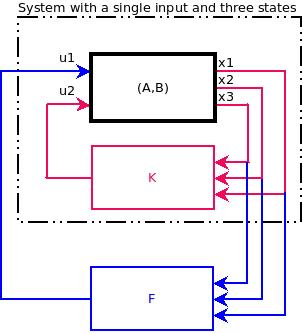
\includegraphics[scale=0.4]{./PolePlacementMI.jpg}
 \caption{Pole placement for a system with multiple inputs} 
\end{figure}
The open loop system is described by:
\begin{equation}
 \dot{\mathbf{x}}=\mathbf{Ax}+\mathbf{b}_1 u_1+\ldots+\mathbf{b}_m u_m
\end{equation}
We single out $\mathbf{b}_{i_0}$ and we rewrite the system as follows:
\begin{equation}
 \dot{\mathbf{x}}=\mathbf{Ax}+\mathbf{B}^{\langle i_0 \rangle} \mathbf{u}^{\langle i_0 \rangle}+\mathbf{b}_{i_0} u_{i_0}
\end{equation}
where $\mathbf{B}^{\langle i_0 \rangle}\in M_{n\times (m-1)}(\mathbb{R})$ is $\mathbf{B}$ without the column $i_0$ and $\mathbf{u}^{\langle i_0 \rangle}\in \mathbb{R}^{m-1}$ is the input vector $\mathbf{u}$ without the input $i_0$. We now determine a feedback $\mathbf{u}^{\langle i_0 \rangle}=\mathbf{K}'\mathbf{x}$ where $\mathbf{K}\in M_{n\times(m-1)}(\mathbb{R})$ so that the closed loop system becomes:
\begin{equation}
 \dot{\mathbf{x}}=(\mathbf{A}+\mathbf{B}^{\langle i_0 \rangle}\mathbf{K}')\mathbf{x}+\mathbf{b}_{i_0} u_{i_0}
\end{equation}
Have we chosen $\mathbf{K}$ so that the pair $(\mathbf{A}+\mathbf{B}^{\langle i_0 \rangle}\mathbf{K}',\mathbf{b}_{i_0})$ is controllable, we can use \hyperlink{prop:AckermansFormula}{Ackerman's formula} to find a state feedback $u_{i_0}=\mathbf{F}'\mathbf{x}$ that places the poles of the overall system to the desired positions. So the only question we have to answer is how do we chose a $\mathbf{K}$ so that $(\mathbf{A}+\mathbf{B}^{\langle i_0 \rangle}\mathbf{K}',\mathbf{b}_{i_0})$ is controllable? This is actually quite simple: we can choose one randomly! The probability that we haven't chosen a proper $\mathbf{K}$ is zero! Let us first give an example of pole placement for a system with 3 states and 3 inputs and afterwards we will explain why we can use almost any $\mathbf{K}$.
\begin{example}[Multiple Inputs: Pole placement]
 Consider the following system with 3 states and 3 inputs:
\begin{equation}
 \dot{\mathbf{x}}=\left[ {\begin{array}{ccc}
      1&-1&2\\3&1&0\\1&4&-1
\end{array} } \right]\mathbf{x}+\left[ {\begin{array}{ccc}     
1&-1&3\\1&2&1\\0&1&5
\end{array} } \right]\mathbf{u}
\end{equation}
where $\mathbf{x},\mathbf{u}\in \mathbb{R}^3$. In particular $\mathbf{u}=\left[ {\begin{array}{ccc}u_1&u_2&u_3\end{array} } \right]'$. It is easy to see that this system is controllable. Let us define the input vector without the third input to be $\mathbf{u}^{\langle3 \rangle}=\left[ {\begin{array}{cc}u_1&u_2\end{array} } \right]'$ (we have chosen $i_0=3$). The the given system is rewritten as:
\begin{equation}
 \dot{\mathbf{x}}=\left[ {\begin{array}{ccc}
      1&-1&2\\3&1&0\\1&4&-1
\end{array} } \right]\mathbf{x}+\left[ {\begin{array}{ccc}     
1&-1\\1&2\\0&1
\end{array} } \right]\mathbf{u}^{\langle3 \rangle}+\left[ {\begin{array}{c}     
3\\1\\5
\end{array} } \right]u_3
\end{equation}
We now choose randomly a $\mathbf{K}\in M_{3\times 2}(\mathbb{R})$ which can be simply:
\begin{equation}
 \mathbf{K}=\left[ {\begin{array}{cc}
1&0\\0&1\\0&0
\end{array} } \right]
\end{equation}
Then using the partial feedback law $\mathbf{u}^{\langle3 \rangle}=\mathbf{K}'\mathbf{x}$ the system becomes:
\begin{equation}
 \dot{\mathbf{x}}=\underbrace{\left[ {\begin{array}{ccc}
      2&-2&2\\4&3&0\\1&5&-1
\end{array} } \right]}_{\mathbf{M}\triangleq\mathbf{A}+\mathbf{B}^{\langle3 \rangle}\mathbf{K}'}\mathbf{x}+\underbrace{\left[ {\begin{array}{c}     
3\\1\\5
\end{array} } \right]}_{\mathbf{H}}u_3
\end{equation}
Assume now that we need to place the poles of the system $(\mathbf{M},\mathbf{H})$ at $-1$, $-2$ and $-3$. Using \hyperlink{prop:AckermansFormula}{Ackerman's formula} we get the feedback law:
\begin{equation}
 u_3=\mathbf{F}'\mathbf{x}
\end{equation}
where
\begin{equation}
 \mathbf{F}=\left[ {\begin{array}{c}
      -2.2018972\\
      -0.7733927\\
      -0.5241832
\end{array} } \right]
\end{equation}
The overall control law then becomes:
\begin{equation}
 \mathbf{u}=\left[ {\begin{array}{c}
      \mathbf{K}' \\ \mathbf{F}'
\end{array} } \right]\mathbf{x}=\left[ {\begin{array}{cc}
      \mathbf{K} & \mathbf{F}
\end{array} } \right]'\mathbf{x}
\end{equation}
\end{example}
As we mentioned earlier, the probability that we choose an inappropriate $\mathbf{K}$ is zero. This is based upon the fact that the family of uncontrollable systems forms a set of measure zero and in nowhere dense inside the set of all systems. This is formally stated as follows \cite{Son98}:
\begin{proposition}
 Let $\mathcal{S}_{n,m}=\{(\mathbf{A},\mathbf{B})\in M_{n}(\mathbb{R})\times M_{n\times m}(\mathbb{R})\}$ and let $\mathcal{S}_{n,m}^{c}$ contain all controllable pairs in $\mathcal{S}_{n,m}$. Then $\mathcal{S}_{n,m}^{c}$ is an open and dense set in $\mathcal{S}_{n,m}$.
\end{proposition}
\begin{proof}
 For a proof and more on topological properties of $\mathcal{S}_{n,m}^{c}$ see \cite{Son98}.
\end{proof}

\section{Stabilizability}
While controllability is necessary (and sufficient) for pole placement, it is not necessary for stabilization. Although we can control the system 100\% and we cannot determine a feedback so as to place the closed loop poles arbitrarily we might be able to find a feedback so that the origin is an asymptotically stable point of the closed loop system. Let us demonstrate this through the following example.
\begin{example}
 The following system is not controllable:
 \begin{equation}
  \dot{\mathbf{x}}=\left[ {\begin{array}{cc}1&2\\0&-2 \end{array} } \right]\mathbf{x}+\left[ {\begin{array}{c}1\\0 \end{array} } \right]u
 \end{equation}
this is obvious since the system is written in the \hyperlink{prop:InputDecoupling}{Kalman input-state decomposition} form. However, if we try the feedback law:
\begin{equation}
 u(\mathbf{x})=\left[ {\begin{array}{cc}-2&0 \end{array} } \right]\mathbf{x}
\end{equation}
Then, the closed loop system is:
 \begin{equation}
  \dot{\mathbf{x}}=\left[ {\begin{array}{cc}-1&2\\0&-2 \end{array} } \right]\mathbf{x}
 \end{equation}
from which it is obvious that its eigenvalues are $-1$ and $-2$ which renders the origin an asymptotically stable point. Trying various other feedbacks we will find out that one of the two eigenvalues of the closed loop system is always $-2$! The second eigenvalue can be placed arbitrarily anywhere on $\mathbb{R}$.
\end{example}
\begin{proposition}[Partial Pole Placement - Exercise]
 Consider an LTI system with $n$ states and $m$ inputs. The rank its controllability matrix is $s<n$. Then:
\begin{enumerate}
 \item Under any linear feedback $\mathbf{u}(\mathbf{x})=\mathbf{K}'\mathbf{x}$, the closed loop system has $n-s$ immovable eigenvalues, namely there is a  $\mathcal{I}=\{\lambda_i\}_{i=1}^{n-s}$ so that:
\begin{equation}
 \mathcal{I}\subset\sigma(\mathbf{A}+\mathbf{BK}') \text{ for all } \mathbf{K}\in M_{n\times m}(\mathbb{R})
\end{equation}
 \item Given a self-conjugate set $\mathcal{J}=\{\lambda_j\}_{j=1}^s$, there is a linear feedback $\mathbf{u}(\mathbf{x})=\mathbf{K}'\mathbf{x}$ with $\mathbf{K}=\left[ {\begin{array}{cc}\mathbf{K}'_1&\mathbf{0}' \end{array} } \right]'$ where $\mathbf{K}_1\in M_{s \times m}(\mathbb{R})$
 \begin{equation}
  \sigma(\mathbf{A}+\mathbf{BK}')=\mathcal{I}\cup \mathcal{J}
 \end{equation}
\end{enumerate}
\end{proposition}
\begin{proof}
 The proof is based on facts that have been explained before and is left to the reader as an exercise. Hint: Use the Kalman input-state decoupled form of the system.
\end{proof}
To this end we give the definition of \emph{stabilizability} which is necessary and sufficient for the existence of a feedback which asymptotically stabilized the closed loop system (renders the origin an asymptotically stable equilibrium point).
\begin{definition}[Asymptotically Stabilizable]\hypertarget{def:stabilizable}
 A control system $\dot{\mathbf{x}}=f(\mathbf{x},\mathbf{u})$ is (asymptotically) stabilizable if there is a feedback law $\mathbf{u}(\mathbf{x})=\rho(\mathbf{x})$ so that the closed loop system $\dot{\mathbf{x}}=f(\mathbf{x},\rho(\mathbf{x}))$ is asymptotically stable.
\end{definition}
\noindent \textbf{Note :} It follows from the definition that if a system is controllable then it is stabilizable. The converse though is not true.
\begin{example}
 Consider a control system in the Kalman input-state decoupled form:
 \begin{equation}
  \dot{\mathbf{x}}=\left[ {\begin{array}{cc}
      \mathbf{A}_{11} & \mathbf{A}_{12} \\ 
      \mathbf{0} & \mathbf{A}_{22}
\end{array} } \right]\mathbf{x}+\left[ {\begin{array}{c}
      \mathbf{B}_{1} \\ 
      \mathbf{0} 
\end{array} } \right]\mathbf{u}
 \end{equation}
where $\mathbf{A}_{11}\in M_{s}(\mathbb{R})$. Let $\mathbf{x}$ be decomposed into its controllable and uncontrollable modes as $\mathbf{x}=\left[ {\begin{array}{cc}\mathbf{x}_{co}' & \mathbf{x}'_{\overline{co}} \end{array} } \right]'$ with $\mathbf{x}_{co}\in\mathbb{R}^s$ and $\mathbf{x}_{\overline{co}}\in\mathbb{R}^{n-s}$ where $s$ is the rank of the controllability matrix of the system.
\begin{eqnarray}
 \dot{\mathbf{x}}_{co}&=&\mathbf{A}_{11}\mathbf{x}_{co}+\mathbf{A}_{12}\mathbf{x}_{\overline{co}}+\mathbf{B}_1\mathbf{u}\label{eqn:113842343}\\
 \dot{\mathbf{x}}_{\overline{co}} &=& \mathbf{A}_{22}\mathbf{x}_{\overline{co}}\label{eqn:uncontrollable2}
\end{eqnarray}
Let us assume that all eigenvalues of $\mathbf{A}_{22}$ have strictly negative real part, i.e. equation (\ref{eqn:uncontrollable2}) has asymptotically stable dynamics. This means that if we denote by $\varphi_{\overline{co}}(t)$ the solution of (\ref{eqn:113842343}) it holds that
$$\|\varphi_{\overline{co}}(t)\|\to 0\text{ as } t\to\infty$$
% On the other hand, the solution of (\ref{eqn:113842343}) with initial condition $\mathbf{x}_{co}(0)=\mathbf{x}_{co}^0$ is given by:
% \begin{eqnarray}
%  \varphi_{co}(t)=e^{\mathbf{A}_{11}t}\mathbf{x}_{co}^0+\int_0^t e^{\mathbf{A}_{11}(t-\tau)}\mathbf{B}_{1}\mathbf{u}(\tau)d\tau+\int_0^t e^{\mathbf{A}_{11}(t-\tau)}\mathbf{A}_{12}\varphi_{\overline{co}}(\tau)d\tau\ \ \label{eqn:00123342}
% \end{eqnarray}
For the controllable pair $(\mathbf{A}_{11},\mathbf{B}_1)$ let us choose a feedback $\mathbf{K}_{1}$ so that the matrix $\mathbf{A}_{11}+\mathbf{B}_1\mathbf{K}'_1$ has all its eigenvalues with negative real part. Applying this feedback to the system yields:
\begin{eqnarray}
 \dot{\mathbf{x}}_{co}&=&(\mathbf{A}_{11}+\mathbf{B}_1\mathbf{K}'_1)\mathbf{x}_{co}+\mathbf{A}_{12}\mathbf{x}_{\overline{co}}\\
 \dot{\mathbf{x}}_{\overline{co}} &=& \mathbf{A}_{22}\mathbf{x}_{\overline{co}}
\end{eqnarray}
Let us now assume that the initial condition of the system is:
\begin{equation}
 \mathbf{x}^{0}=\left[ {\begin{array}{c}
      \mathbf{x}_{co}^0 \\ 
      \mathbf{x}_{\overline{co}}^0
\end{array} } \right]
\end{equation}
then the trajectory of the closed loop system is:
\begin{equation}
 \varphi(t)=\left[ {\begin{array}{c}
      \varphi_{co}(t) \\ 
      \varphi_{\overline{co}}(t)
\end{array} } \right]=
\left[ {\begin{array}{c}
      e^{(\mathbf{A}_{11}+\mathbf{B}_1\mathbf{K}'_1)t}\mathbf{x}_{co}^0+\int_0^t e^{(\mathbf{A}_{11}+\mathbf{B}_1\mathbf{K}'_1)t}\mathbf{A}_{12}\varphi_{\overline{co}}(\tau)d\tau \\ 
      e^{\mathbf{A}_{22}t}\mathbf{x}_{\overline{co}}^0
\end{array} } \right]
\end{equation}
Notice that $\varphi(t)$ converges to the origin from any initial point (why?).
\end{example}

\noindent We now state the following stabilizability criterion \cite{Hes09}:
\begin{proposition}[Popov-Belevitch-Hautus Stabilizability Criterion]\hypertarget{PopovStabilizability}
 The following conditions are equivalent:
\begin{enumerate}
 \item The pair $(\mathbf{A},\mathbf{B})$ is stabilizable.
\item $\operatorname{rank} \left[ {\begin{array}{c|c} \lambda\mathbf{I}-\mathbf{A} & \mathbf{B} \end{array} } \right]=n$ for all $\lambda\in\mathbb{C}$ with non-negative real part.
 \item $\operatorname{rank} \left[ {\begin{array}{c|c} \lambda\mathbf{I}-\mathbf{A} & \mathbf{B} \end{array} } \right]=n$ for all $\lambda\in\mathbb{C}$ that are eigenvalues of $\mathbf{A}$ and have non-negative real part.
\end{enumerate}
\end{proposition}
\noindent \textbf{Note :} Given a $\lambda\in\mathbb{C}$ with $\operatorname{re}(\lambda)\geq 0$, 
the condition that $\operatorname{rank} \left[ {\begin{array}{c|c} \lambda\mathbf{I}-\mathbf{A} & \mathbf{B} \end{array} } \right]=n$
suggests that there is no nonzero vector $\mathbf{z}$ such that
\begin{eqnarray}
&&\left[ {\begin{array}{c|c} \lambda\mathbf{I}-\mathbf{A} & \mathbf{B} \end{array} } \right]' \mathbf{z}=\mathbf{0}\\
&\Leftrightarrow& \left[ {\begin{array}{c} \lambda\mathbf{I}-\mathbf{A}' \\ \mathbf{B}' \end{array} } \right] \mathbf{z}=\mathbf{0}
\end{eqnarray}
Therefore, if $\mathbf{z}$ is such that $(\lambda\mathbf{I}-\mathbf{A}')\mathbf{z}=\mathbf{0}$, i.e.
$\mathbf{z}$ is an eigenvector of $\mathbf{A}'$ associated with the eigenvalue $\lambda$, then
$\mathbf{B}'\mathbf{x}\neq\mathbf{0}$, i.e. $\mathbf{z}\notin\operatorname{ker}\mathbf{B}'$.
Once again, it should be mentioned that $\mathbf{A}$ and $\mathbf{A}'$ have the same eigenvalues.
This leads to the following corollary:
\begin{corollary}
 The pair $(\mathbf{A},\mathbf{B})$ is stabilizable if no eigenvector of $\mathbf{A}'$
 is in $\operatorname{ker}\mathbf{B}'$.
\end{corollary}

\noindent Another result, which is due to Wonham, provides an approach to stabilizability through \hyperlink{def:cyclicMatrix}{cyclicity}. Let $\mu\in\mathbb{R}[t]$ be the minimal polynomial of $\mathbf{A}$. This polynomial can be factored as follows:
\begin{equation}
 \mu(t)=\mu^+(t)\mu^-(t)
\end{equation}
where $\mu^+(t)$ has all its roots in the closed right half open plane and $\mu^-(t)$
is a polynomial with all its roots in the open left half plane. Let us define the set
\begin{equation}
 E^+ = \left\{ \mathbf{x}\in\mathbb{R}^n,\ \mu^+(\mathbf{A})\mathbf{x}=0\right\}
\end{equation}
\begin{theorem}
 The pair $(\mathbf{A},\mathbf{B})$ is stabilizable if and only if the range of $\mathcal{C}(\mathbf{A},\mathbf{B})$
contains $E^+$.
\end{theorem}
\begin{proof}
 For the proof see \cite{Won67}.
\end{proof}


%
%
%
% Lyapunov theory
%
%
\section{Lyapunov Theory}
%
% Introduction to Lyapunov Theory
%
Lyapunov theory splits into two categories. Firstly, the direct Lyapunov theory applies on linear and nonlinear systems to provide results on the stability properties of their equilibrium points (assumed to be the origin). The direct approach tackles the system \emph{as is} without any transformations of approximations. Second, the indirect approach offers local stability results regarding the linearization of a nonlinear system around an equilibrium point. This approach uses mainly tools from linear systems theory but is more limited compared to the direct approach.
%
% DIRECT LYAPUNOV THEORY
%
\subsection{Direct Lyapunov Theory}
We first give the definition of a directional derivative (or \emph{Lie derivative}) along the trajectories of a dynamical system:
%
% Lie derivative
%
\begin{definition}[Derivative along the trajectories of a system]
 Given a dynamical system $\Sigma:\dot{\mathbf{x}}(t)=f(\mathbf{x}(t))$, where $f:\mathbb{R}^n\to\mathbb{R}^n$, and a function $V:\mathbb{R}^n\to\mathbb{R}$ we define the derivative of $V$ along the trajectories of the system $\Sigma$ as:
 \begin{equation}
  \left.\frac{dV}{dt}\right|_{\Sigma} \equiv  \left.\frac{dV}{dt}\right|_{\mathbf{x}(t)} = 
\left( \frac{\partial V}{\partial \mathbf{z}}\cdot f(\mathbf{z}) \right)_{\mathbf{z}=\mathbf{x}(t)}
 \end{equation}
\end{definition}
%
% Notation
% 
\noindent \textbf{Notation :} Various notational schemes have been adopted by different authors. Some of the most widely used are $(L_f V)(\mathbf{x})$ and $\dot{V}(\mathbf{x})$. The former is the most concise and clear in my opinion.
%
%
% Lie Derivative Example #1
%
\begin{example}
 Consider the LTI system $\Sigma:\dot{\mathbf{x}}=\mathbf{Ax}$ and the function $V(\mathbf{z})=\mathbf{z}'\mathbf{Pz}$ where $\mathbf{P}\in \mathcal{S}_n(\mathbb{R})$ is a symmetric matrix. The Lie derivative of $V$ along the trajectories of $\Sigma$ is calculated as follows:
\begin{eqnarray}
 \left.\frac{dV}{dt}\right|_{\mathbf{x}(t)} &=& \left. \frac{d\left( \mathbf{z}'\mathbf{Pz} \right)}{dt} \right|_{\mathbf{z}=\mathbf{x}(t)}\\
&=& \dot{\mathbf{x}}'\mathbf{Px}+\mathbf{x}'\mathbf{P}\dot{\mathbf{x}}\\
&=& \mathbf{x}'\mathbf{A}'\mathbf{Px}+\mathbf{x}'\mathbf{PAx}\label{eqn:314159265358979323}\\
&=& \mathbf{x}'(\mathbf{A}'\mathbf{P}+\mathbf{PA})\mathbf{x}
\end{eqnarray}
Recall that every scalar is equal to its transpose, so for example for any vector $\mathbf{y}\in\mathbb{R}^n$ and any matrix $\mathbf{Q}\in M_n(\mathbb{R})$, it is true that $\mathbf{y}'\mathbf{Qy}=(\mathbf{y}'\mathbf{Qy})'=\mathbf{y}'\mathbf{Q}'\mathbf{y}$. Therefore, equation (\ref{eqn:314159265358979323}) becomes:
\begin{eqnarray}
 \mathbf{x}'\mathbf{A}'\mathbf{Px}+\mathbf{x}'\mathbf{PAx} &=& (\mathbf{x}'\mathbf{A}'\mathbf{Px})'+\mathbf{x}'\mathbf{PAx}\\
&=&\mathbf{x}'\mathbf{P}'\mathbf{Ax}+\mathbf{x}'\mathbf{PAx}\\
&=&\mathbf{x}'(\mathbf{P}'+\mathbf{P})\mathbf{A}\mathbf{x}
\end{eqnarray}
But, since $\mathbf{P}$ is assumed to be symmetric, one has that:
\begin{eqnarray}
 \left.\frac{dV}{dt}\right|_{\mathbf{x}(t)} &=& 2\mathbf{x}'\mathbf{PAx}
\end{eqnarray}
We will end up with the same result if we use the fact that $\frac{dV}{dt}|_\Sigma= L_f V = \frac{\partial V}{\partial \mathbf{x}} f(\mathbf{x})$. In particular we have:
\begin{equation}
 \frac{\partial V(\mathbf{x})}{\partial \mathbf{x}}=\frac{\partial (\mathbf{x}'\mathbf{Px})}{\partial\mathbf{x}}=\mathbf{x}'(\mathbf{P}+\mathbf{P}')=2\mathbf{x}'\mathbf{P}
\end{equation}
Hence:
\begin{equation}
 \left.\frac{dV}{dt}\right|_{\Sigma} = (L_f V)(\mathbf{x})=2\mathbf{x}'\mathbf{PAx}
\end{equation}

\end{example}
%
% Note #1 on example #1:
%
\noindent \textbf{Note 1:} Note that nowhere did we have to calculate explicitly the trajectory of the system in order to come up with the Lie derivative of $V$ along the trajectories of the system.\\
\\
%
% Note #2 on example #1
%
\noindent \textbf{Note 2:} The fact that $2\mathbf{x}'\mathbf{PAx}=\mathbf{x}'(\mathbf{A}'\mathbf{P}+\mathbf{PA})\mathbf{x}$ in no way does it imply that $2\mathbf{PA}=\mathbf{A}'\mathbf{P}+\mathbf{PA}$! Also, if $\mathbf{P}$ is assumed to be symmetric (and $\mathbf{A}$ does not possess any special structure as usually is the case), then $\mathbf{A}'\mathbf{P}+\mathbf{PA}$ is also symmetric, while $\mathbf{PA}$ is not guaranteed to be so. If we have to choose between these two we should definitely go for the second one. Symmetric matrices are rich in properties that facilitate algebraic manipulations. For instance, symmetric matrices have only real eigenvalues, they are always diagonalizable and specifically we can choose their eigenvectors to form an orthonormal basis for $\mathbb{R}^n$. I guess the trick is already clear... Given any quadratic form $V(\mathbf{x})=\mathbf{x}'\mathbf{Qx}$ we can convert it to a symmetric form as follows:
\begin{equation}
 V(x)=\mathbf{x}'\mathbf{Qx}=\mathbf{x}'\frac{\mathbf{Q}+\mathbf{Q}'}{2}\mathbf{x}=\mathbf{x}'\tilde{\mathbf{Q}}\mathbf{x}
\end{equation}
The matrix $\tilde{\mathbf{Q}}=\frac{1}{2}(\mathbf{Q}+\mathbf{Q}')$ is symmetric. Let us close this note with the following equation:
\begin{equation}
 (L_f V)(\mathbf{x})=2\mathbf{x}'\mathbf{PA}\mathbf{x}=2\mathbf{x}'\frac{(\mathbf{PA})'+\mathbf{PA}}{2}\mathbf{x}=\mathbf{x}'(\mathbf{A}'\mathbf{P}+\mathbf{PA})\mathbf{x}
\end{equation}

%
%
%
% Lie derivative example #2
%
\begin{example}
 In this example we will be a bit more explicit. Consider the dynamical system given by:
 \begin{equation}\label{eqn:42123434234}
  \frac{d}{dt}\left[ {\begin{array}{c} x_1\\x_2 \end{array} } \right]=\left[ {\begin{array}{c} x_2\\-2x_2-x_1 \end{array} } \right]=\mathrel{:}f(x_1,x_2)
 \end{equation}
and the function $V:\mathbb{R}^2\to\mathbb{R}$ given by:
\begin{equation}
 V(\mathbf{x})=V(x_1,x_2)=\frac{1}{2}(x_1^2+x_2^2)=\frac{1}{2}\mathbf{x}'\mathbf{x}
\end{equation}
The derivative of $V$ is:
\begin{equation}
 \frac{\partial}{\partial \mathbf{x}}V(\mathbf{x})=\left[ {\begin{array}{cc} \frac{\partial V(x_1,x_2)}{\partial x_1}&\frac{\partial V(x_1,x_2)}{\partial x_2} \end{array} } \right]=\left[ {\begin{array}{cc} x_1&x_2 \end{array} } \right]
\end{equation}
And the Lie derivative of $V$ along the trajectories of (\ref{eqn:42123434234}) is the function $\dot{V}:\mathbb{R}^2\to\mathbb{R}$ given by:
\begin{equation}
 \dot{V}(x_1,x_2)=\left[ {\begin{array}{cc} x_1&x_2 \end{array} } \right]\cdot \left[ {\begin{array}{c} x_2\\-2x_2-x_1 \end{array} } \right]=-2x_2^2
\end{equation}
\end{example}
\noindent \textbf{Property of $L_f V$ :} The solution of the time-invariant nonlinear system $\dot{\mathbf{x}}=f(\mathbf{x})$ with initial condition $\mathbf{x}(0)=\mathbf{x}_0$ is denoted as $\varphi(t,\mathbf{x}_0)$. Then it holds that for all $t\geq 0$:
\begin{equation}
 V(\varphi(t,\mathbf{x}_0))-V(\varphi(0,\mathbf{x}_0))=\int_0^t \dot{V}(\varphi(\tau,\mathbf{x}_0))d\tau
\end{equation}
which is simply written as:
\begin{equation}
 V(\varphi(t,\mathbf{x}_0))-V(\mathbf{x}_0)=\int_0^t \dot{V}(\varphi(\tau,\mathbf{x}_0))d\tau \label{eqn:33129076824}
\end{equation}
\\
We need a couple of more definitions before stating the main result of this section. The notion of \emph{positive (semi)definite} functions extends the notion of (non-negative) positive numbers on $\mathbb{R}$.
%
% Positive (Semi)definite function.
%
\begin{definition}[Positive (semi)definite function]
 A function $V:D\to\mathbb{R}$, where $D\subseteq\mathbb{R}^n$ is said to be positive semidefinite if $V(\mathbf{0})=0$ and for every $\mathbf{x}\in D$ it holds that $V(\mathbf{x})\geq 0$. It is called positive definite if additionally for every $\mathbf{x}\in D-\{0\}$ it is true that $V(\mathbf{x})>0$. A function $V$ is called negative (semi)definite if $-V$ is positive (semi)definite.
\end{definition}
\noindent \textbf{Note :} Candidate positive definite functions are in many cases quadratic functions, that is functions of the form $V(\mathbf{x})=\mathbf{x}'\mathbf{Qx}$ where $\mathbf{Q}\in M_n(\mathbb{R})$ is an appropriate matrix.
%
% Positive (semi)definite Matrix
%
\begin{definition}[Positive (semi)definite matrix]
 A matrix $\mathbf{Q}\in M_n(\mathbb{R})$ is called positive (semi)definite if the corresponding quadratic function $V(\mathbf{x})=\mathbf{x}'\mathbf{Qx}$ is positive (semi)definite.
\end{definition}
An algebraic criterion exists to test whether a given symmetric matrix is positive definite or positive semidefinite.
%
% Proposition: Positive Def. Matrix <=> Positive eigenvalues
%
\begin{proposition}[Criterion for Positive Semi-definiteness]
 Let $\mathbf{Q}\in M_n(\mathbb{R})$ be a symmetric matrix - we denote by $\mathcal{S}_n(\mathbb{R})$ the set of all symmetric matrices in $M_n(\mathbb{R})$. Then, it is positive semi-definite if and only if all its eigenvalues are (non-negative)positive.
\end{proposition}
%
% Proof of the proposition...
\begin{proof}
 1. ($\Rightarrow$) We first prove that if $\mathbf{Q}$ is symmetric and positive semidefinite, then all its eigenvalues are non-negative. Recall from linear algebra that a symmetric matrix has only real eigenvalues, thus we can compare them with $0$. If $\lambda\in\mathbb{R}$ is an eigenvalue of $\mathbf{Q}$ and $\mathbf{v}\in\mathbb{R}^n$ is the corresponding eigenvector, then $\mathbf{Qv}=\lambda\mathbf{v}$. Left-multiplying by $\mathbf{v}'$ yields:
 \begin{eqnarray}
  &&\mathbf{v}'\mathbf{Qv}=\lambda\mathbf{v}'\mathbf{v}\\
&\Rightarrow& \lambda=\frac{\mathbf{v}'\mathbf{Qv}}{\mathbf{v}'\mathbf{v}}=\frac{\mathbf{v}'\mathbf{Qv}}{\|\mathbf{v}\|_2^2}\geq 0
 \end{eqnarray}
Note that the division by $\mathbf{v}'\mathbf{v}=\|\mathbf{v}\|_2^2$ is allowed since $\mathbf{v}\neq \mathbf{0}$.\\
\\
2. ($\Leftarrow$) We now prove that if all eigenvalues of the symmetric $\mathbf{Q}$ are non-negative, then the matrix is positive semi-definite. It is known that symmetric matrices can be diagonalized by a unitary matrix $\mathbf{U}\in\mathcal{U}_n(\mathbb{R})$, i.e. if $\mathbf{\Lambda}\in\mathfrak{dg}(n,\mathbb{R})$ is the diagonal matrix of eigenvalues of $\mathbf{Q}$, then there is a unitary matrix $\mathbf{U}$ so that:
\begin{equation}
 \mathbf{Q}=\mathbf{U}^{-1}\mathbf{\Lambda U}=\mathbf{U}'\mathbf{\Lambda U}
\end{equation}
 This means that the column-vectors of $\mathbf{U}$, namely $\mathbf{u}_1,\mathbf{u}_2,\ldots,\mathbf{u}_n$, are eigenvectors of $\mathbf{Q}$. These eigenvectors form an orthonormal basis or $\mathbb{R}^n$ (i.e. $\|\mathbf{u}_i\|=1$ and $\mathbf{u}'_i\mathbf{u}_j=0$ for $i\neq j$), so any vector $\mathbf{x}\in\mathbb{R}^n$ can be represented as a linear combination:
\begin{equation}
 \mathbf{x}=\sum_{i=1}^n\alpha_i\mathbf{u}_i
\end{equation}
 Let $\lambda_i$ denote the eigenvalue that corresponds to $\mathbf{u}_i$. We now calculate the following:
\begin{eqnarray}
 \mathbf{x}'\mathbf{Qx}&=&\sum_{i=1}^n\sum_{j=1}^n\alpha_i\alpha_j\mathbf{u}'_i\mathbf{Qu}_j\\
&=&\sum_{i=1}^n\sum_{j=1}^n\alpha_i\alpha_j\lambda_j\mathbf{u}'_i\mathbf{u}_j\\
&=&\sum_{i=1}^n\alpha_i^2\lambda_i\mathbf{u}'_i\mathbf{u}_i\\
&=&\sum_{i=1}^n\alpha_i^2\lambda_i\|\mathbf{u}_i\|_2^2
\end{eqnarray}
From this we conclude that $\mathbf{x}'\mathbf{Qx}\geq 0$ for all $\mathbf{x}$ if and only if $\lambda_i\geq 0$ for $i=1,2,\ldots,n$.
\end{proof}
%
% Proposition: L'L is positive semidefinite
%
\begin{proposition}[Exercise]
 If $\mathbf{L}\in M_n(\mathbb{R})$ is any matrix, then $\mathbf{Q}\triangleq \mathbf{L}'\mathbf{L}$ is symmetric and positive semidefinite.
\end{proposition}
\begin{proof}
 This proposition provides a way to construct positive semidefinite matrices. proposition is left to the reader as an exercise.
\end{proof}
%
% Cholesky factorization
%
\begin{theorem}[Cholesky factorization]\label{thm:cholesky}\hypertarget{thm:cholesky}
 Let $\mathbf{Q}$ be a \textbf{symmetric} and \textbf{positive definite} matrix. Then, there is a unique lower triangular matrix $\mathbf{L}$ with strictly positive diagonal entries such that $\mathbf{Q}=\mathbf{LL}'$. If $\mathbf{Q}$ is a \textbf{positive semidefinite} and \textbf{symmetric} matrix then the uniqueness of $\mathbf{L}$ is dropped and the diagonal entries of $\mathbf{L}$ are non-negative.
\end{theorem}
%
%
% Practical notation for positive (semi)definiteness
%
\noindent \textbf{Notation :} We adopt the following practical notation for positive and negative (semi)definite matrices. If $\mathbf{A}$ is a positive semidefinite matrix, we write $\mathbf{A}\succeq 0$ while if it is positive definite we write $\mathbf{A}\succ 0$. For negative matrices we use the notation $\mathbf{A}\preceq 0$ and $\mathbf{A}\prec 0$ respectively. The symbol $\mathbf{A}\succeq \mathbf{B}$ should be interpreted as $\mathbf{A}-\mathbf{B}\succeq 0$ (The matrix $\mathbf{A}-\mathbf{B}$ is positive semidefinite). We need to underline that $\succeq$ is not a partial order in $M_n(\mathbb{R})$, i.e. there are pairs of matrices $\mathbf{A}$ and $\mathbf{B}$ such that neither $\mathbf{A}\succeq \mathbf{B}$ nor $\mathbf{B}\succeq \mathbf{A}$. \\
\\
The \hyperlink{thm:cholesky}{Cholesky factorization} theorem allows us to prove that a symmetric and positive definite quadratic form defines a vector norm while a symmetric and positive semidefinite one defines a seminorm. For completeness we provide first the definition of a vector norm and a vector seminorm.
\begin{definition}[Norm/Seminorm]
 A mapping $\|\cdot\|:\mathbb{R}^n\ni\mathbf{x}\mapsto\|\mathbf{x}\|\in[0,\infty)$ is called a (vector) norm if it satisfies the following properties:
\begin{enumerate}
 \item For every $\alpha\in\mathbb{R}$ it holds that $\|\alpha\mathbf{x}\|=|\alpha|\|\mathbf{x}\|$
 \item For all $\mathbf{x},\mathbf{y}\in\mathbb{R}^n$ it is $\|\mathbf{x}+\mathbf{y}\|\leq\|\mathbf{x}\|+\|\mathbf{y}\|$
 \item $\|\mathbf{x}\|=0 \implies \mathbf{x}=\mathbf{0}$
\end{enumerate}
If the third property is dropped, then the mapping is called a seminorm.
\end{definition}
We are already familiar with various norms in $\mathbb{R}^n$ the most widely used one being the Euclidean norm denoted as $\|\cdot\|_2$. The Euclidian norm is defined as $\|\mathbf{x}\|_2=\sqrt{\mathbf{x}'\mathbf{x}}$. Norms are useful because they allow us to define and study convergence in vector spaces. We have previously clarified what we mean when we say that the trajectory of a linear system converges to $\mathbf{0}$ in the sense of $\|\cdot\|_2$. It is:
\begin{equation}
 \lim_{t\to\infty}\varphi(t,\mathbf{x}_0)=\mathbf{0}\Leftrightarrow \lim_{t\to\infty}\|\varphi(t,\mathbf{x}_0)\|_2=0
\end{equation}
Where the left-hand side equation has no meaning whatsoever unless we specify that the convergence is meant in the $\|\cdot\|_2$-sense.
Imagine now that someone tells us that a trajectory converges to $\mathbf{0}$ in the $\|\cdot\|_\omega$ sense, where $\|\cdot\|_\omega$ is some other norm. Should we assume that it converges in the $\|\cdot\|_2$-sense as well. The answer is positive if and only if the two norms are \emph{equivalent}. Here is the definition of equivalent norm:
\begin{definition}[Equivalent norms]
 Let $\|\cdot\|_\alpha$ and $\|\cdot\|_\beta$ be two norms in $\mathbb{R}^n$. The two norms are called equivalent if there are numbers $m,M\geq 0$ so that for all $\mathbf{x}\in\mathbb{R}^n$ it holds:
\begin{equation}
 m\|\mathbf{x}\|_\alpha \leq \|\mathbf{x}\|_\beta \leq M\|\mathbf{x}\|_\alpha
\end{equation}
\end{definition}

We now prove that positive definite quadratic forms, i.e. functions of the form $f(\mathbf{x})=\mathbf{x}'\mathbf{Px}$ where $\mathbf{P}\succ 0$ induce norms.
\begin{proposition}
 Let $\mathbf{P}\in \mathcal{S}_n(\mathbb{R})$ with $\mathbf{P}'=\mathbf{P}\succ 0$. The mapping $\|\cdot\|_\mathbf{P}:\mathbb{R}\to [0,\infty)$ defined by:
\begin{equation}
 \|\mathbf{x}\|_\mathbf{P}=\sqrt{\mathbf{x}'\mathbf{Px}}
\end{equation}
is a vector norm in $\mathbb{R}$. If $\mathbf{P}\succeq 0$, then $\|\cdot\|_\mathbf{P}$ is a seminorm.
\end{proposition}
\begin{proof}
 Assume first that $\mathbf{P}$ is symmetric and positive definite. Then, there is a unique lower triangular matrix $\mathbf{L}$ with strictly positive diagonal entries (Cholesky factorization theorem) so that $\mathbf{P}=\mathbf{LL}'$. Then:
\begin{equation}
 \|\mathbf{x}\|_\mathbf{P}=\sqrt{\mathbf{x}'\mathbf{Px}}=\sqrt{\mathbf{x}'\mathbf{LL}'\mathbf{x}}=\sqrt{(\mathbf{L}'\mathbf{x})'(\mathbf{L}'\mathbf{x})}=\|\mathbf{L}'\mathbf{x}\|_2
\end{equation}
For $\alpha\in\mathbb{R}$ we have:
\begin{equation}
 \|\alpha\mathbf{x}\|_\mathbf{B}=\|\alpha\mathbf{L}'\mathbf{x}\|_2=|\alpha|\|\mathbf{L}'\mathbf{x}\|_2=|\alpha|\|\mathbf{x}\|_\mathbf{P}
\end{equation}
Second, let $\mathbf{x},\mathbf{y}\in\mathbb{R}^n$. Then:
\begin{equation}
 \|\mathbf{x}+\mathbf{y}\|_\mathbf{P}=\|\mathbf{L'}\mathbf{x}+\mathbf{L}'\mathbf{y}\|_2\leq\|\mathbf{L}'\mathbf{x}\|_2+\|\mathbf{L}'\mathbf{y}\|_2=\|\mathbf{x}\|_\mathbf{P}+\|\mathbf{y}\|_\mathbf{P}
\end{equation}
The third property of the vector norm accrues from the fact that $\mathbf{L}$ being a lower triangular matrix with strictly positive diagonal entries implies that it is invertible, hence $\operatorname{ker}\mathbf{L}=\{\mathbf{0}\}$. Therefore:
\begin{equation}
 \|\mathbf{x}\|_\mathbf{P}=0\Rightarrow\|\mathbf{L}'\mathbf{x}\|_2=0\Rightarrow \mathbf{L}'\mathbf{x}=\mathbf{0}\Rightarrow\mathbf{x}\in \operatorname{ker}\mathbf{L}'=\{\mathbf{0}\}
\end{equation}
This last property does not hold if $\mathbf{L}$ is lower triangular with a zero element in its diagonal. The determinant of a triangular matrix equals the product of its diagonal elements. In that case it would be $|\mathbf{L}|=|\mathbf{L}'|=0$ rendering the matrix non-invertible. Then the kernel of $\mathbf{L}'$ would have dimension at least one and there are non-zero vectors such that $\mathbf{L}'\mathbf{x}=\mathbf{0}$.
\end{proof}

%
% LYAPUNOV THEOREM (Direct)
%
We are now ready to state and prove the main result of this section (The proof can be also found in \cite{Kha02}):
\begin{theorem}[Lyapunov stability theorem]\hypertarget{lst}
 Let $\mathbf{x}=\mathbf{0}$ be an equilibrium point for the system $\dot{\mathbf{x}}=f(\mathbf{x})$ with $\mathbf{x}\in\mathbb{R}^n$ and $D\subseteq \mathbb{R}^n$ with $D\ni \mathbf{0}$. The vector field $f$ is locally Lipschitz (so that the differential equation admits unique solutions). Let $V:D\to[0,\infty)$ be a continuously differentiable function such that:
\begin{enumerate}
 \item  $V$ is positive definite in $D$.
 \item  $L_f V$ is negative semidefinite in $D$.
\end{enumerate}
then $\mathbf{x}=\mathbf{0}$ is \hyperlink{stability-definition}{stable}. If additionally $L_f V$ is negative definite in $D$, then the origin is \hyperlink{definition:LAS}{locally asymptotically stable}.
\end{theorem}
% PROOF of Lyapunov's theorem
\begin{proof}
 For any $\varepsilon>0$ take $r\in (0,\varepsilon]$ such that:
\begin{equation}
 \mathcal{B}_r(\mathbf{0})\triangleq \{\mathbf{x}\in\mathbb{R}^n | \|\mathbf{x}\|\leq r \}\subset D
\end{equation}
Let $\alpha\triangleq \min_{\|\mathbf{x}\|=r}V(\mathbf{x})$. $V$ is positive definite so $\alpha>0$. Take a $\beta \in (0,\alpha)$ and define the set:
\begin{equation}
 \Omega_\beta = \{\mathbf{x}\in \mathcal{B}_r | V(\mathbf{x}) \leq \beta \}
\end{equation}
The trajectory of the system starting inside $\Omega_\beta$ will remain in $\Omega_\beta$ for all future times $t\geq 0$. This is a consequence of condition \#2. To corroborate this claim we use equation (\ref{eqn:33129076824}). Let $\mathbf{x}_0 \in \Omega_\beta$ and $\varphi(t,\mathbf{x}_0)$ be the trajectory starting from $\mathbf{x}_0$. Then
\begin{equation}
 V\left( \varphi\left( t,\mathbf{x}_0\right) \right)-V(\mathbf{x}_0)=\int_0^t \left( L_fV\right) \left( \varphi(\tau,\mathbf{x}_0)\right) d\tau\leq 0
\end{equation}
That is, for all $t\geq 0$:
\begin{equation}
 V(\varphi(t,\mathbf{x}_0))\leq V(\mathbf{x}_0)\leq \beta \Rightarrow\varphi(t,\mathbf{x}_0)\in\Omega_\beta 
\end{equation}
Since $V$ is continuous and $V(\mathbf{0})=0$, $\Omega_\beta\ni\mathbf{0}$ and we can find a $\delta>0$ so that:
\begin{equation}
 \mathcal{B}_\delta \subset \Omega_\beta \subset \mathcal{B}_r
\end{equation}
Which further means that any trajectory starting from $\mathcal{B}_\delta$ (i.e. from inside $\Omega_\beta$) will remain in $\Omega_\beta$ thus it will remain in $\mathcal{B}_r$. Formally speaking:
\begin{equation}
 \mathbf{x}(0)=\mathbf{x}_0 \in \mathcal{B}_\delta \Rightarrow \mathbf{x}_0 \in \Omega_\beta \Rightarrow \varphi(t;\mathbf{x}_0) \in \Omega_\beta
\Rightarrow \varphi(t;\mathbf{x}_0) \in \mathcal{B}_r
\end{equation}
The same thing in norm notation:
\begin{equation}
 \|\mathbf{x}_0\|<\delta \Rightarrow \|\varphi(t;\mathbf{x}_0)\| < r \leq \varepsilon \text{ for all } t\geq 0
\end{equation}
which states exactly that the origin is a stable equilibrium. We shall now prove the second part of the theorem regarding asymptotic stability. We need to show that:
\begin{equation}
 \lim_{t\to\infty}\|\varphi(t,\mathbf{x}_0)\|=0\label{normConvergence}
\end{equation}
whenever $L_f V$ is negative definite.
Or equivalently that for all $\varepsilon>0$, there is a $t_0=t_0(\varepsilon)>0$ 
such that $\|\varphi(t,\mathbf{x}_0)\|<\varepsilon$ for all $t>t_0$. Since for every
$\varepsilon>0$ there is an $\varepsilon'>0$ such that $\Omega_{\varepsilon'}\subseteq \mathcal B_\varepsilon$,
it suffices to show that 
\begin{equation}
 \lim_{t\to\infty}V\left(\varphi(t,\mathbf{x}_0)\right)=0\label{lyapConvergence}
\end{equation}
In other words the norm-convergence described by (\ref{normConvergence}) is equivalent to the
convergence in terms of $V$ as it is described by (\ref{lyapConvergence}).

Since $L_f V$ is negative definite, $V(\varphi(t;\mathbf{x}_0))$ is strictly decreasing with
respect to $t$ and since $V$ is positive definite, there is a $c\geq 0$ such that
$\lim_{t\to\infty}V\left(\varphi(t,\mathbf{x}_0)\right)=c$. We need to show that $c=0$.
Let us assume that $c>0$. We then may find a ball of radius $d>0$ such that $\mathcal B_d\subseteq \Omega_c$.
Since $\lim_{t\to\infty}V\left(\varphi(t,\mathbf{x}_0)\right)=c$, the trajectory $\varphi(t,\mathbf{x}_0)$
is outside $\mathcal B_d$ for all $t\geq 0$. Let $\gamma\triangleq -\max_{d\leq \|\mathbf{x}\| \leq r}
L_f V(\mathbf{x})$. Since $L_f V\prec 0$, it is $\gamma>0$. Then,
\begin{eqnarray}
 V\left(\varphi(t,\mathbf{x}_0)\right) &=& 
V\left(\mathbf{x}_0\right)+
\int_0^t L_f V(\varphi(\tau,\mathbf{x}_0))d\tau\\
&\leq& V\left(\mathbf{x}_0\right)-\gamma t
\end{eqnarray}
Then, for all $t>V\left(\mathbf{x}_0\right)/\gamma$, it is $V\left(\mathbf{x}_0\right)-\gamma t<0$, 
therefore $V\left(\varphi(t,\mathbf{x}_0)\right)<0$ which contradicts the fact that $V$ is positive
definite. Therefore $c=0$.
\end{proof}

\noindent \textbf{Note :} A function $V$ that is positive definite over $D$ is called a 
\emph{candidate Lyapunov function}. If additionally $L_fV$ is negative semidefinite, then
$V$ is called a \emph{Lyapunov function}. If $L_fV$ is negative definite, $V$ is said to 
be a \emph{string Lyapunov function}.


\subsection{La Salle's Invariance Principle}
Sometimes we are able to determine a positive definite function $V$ but $L_f V$
is only negative semidefinite instead of negative definite, therefore we may conclude only
that the system into consideration is stable but not asymptotically stable. The fact that
our $L_f V$ is only negative semidefinite does not suggest that our system is not 
asymptotically stable. If it is, however, we cannot prove it which is a great pity 
because we were so close! This is where \emph{La Salle's invariance principle} chimes in.

Let us start with such a motivating example. The following state space model
(nonlinear, time invariant) describes the dynamics of a pendulum with linear friction term:
\begin{equation}\label{pendulum_friction}
 \frac{d}{dt}
\left[ {\begin{array}{c}
x_1  \\
 x_2 
 \end{array} } \right]=
\left[ {\begin{array}{cc}
 x_2  \\
 -kx_2-\sin x_1
 \end{array} } \right]
\end{equation}
defined on the domain $D=[-\pi,\pi]\times\mathbb{R}\ni \mathbf{x}$.
The total energy of the system is chosen as a candidate Lyapunov function; this is:
\begin{equation}
 V(\mathbf{x})=\frac{1}{2}x_2^2-\cos x_1+1
\end{equation}
$V$ is positive definite over all $\mathbf{x}\in D$. Then, we compute that $L_f V (\mathbf{x})=-kx_2^2$
and it is $L_f V \preceq 0$. In fact it is $(L_f V)(\mathbf{x})=0$ if and only if $x_2=0$.

Although it is possible to
calculate analytically the solution of (\ref{pendulum_friction}) and corroborate that the
origin is an asymptotically stable point, Lyapunov's theorem fails to prove asymptotic 
stability (by means of a completely intuitive Lyapunov function). In what follows we 
state and prove a complementary result to Lyapunov's stability theorem, known as La Salle’s 
(invariance) Principle. This is used in a combination with standard Lyapunov-like theorems to 
derive asymptotic stability properties of nonlinear systems when
the Lie derivative of the candidate Lyapunov function (along the trajectory of the system) is merely negative
semidefinite (and not negative definite).

\begin{definition}[Positive Invariant Set]\hypertarget{def:positiveInvariant}
 A set $M\subseteq \mathbb{R}^n$ is called positive invariant with respect to the system
$\dot{\mathbf{x}}=f(\mathbf{x})$ if for every $\mathbf{x}_0\in M$ and for every $t\geq 0$,
it holds that $\varphi(t;\mathbf{x}_0)\in M$.
\end{definition}
Any trajectory that starts from a point in $M$ remains in $M$ at all future times.
A trivial invariant set is $M=\mathbb{R}^n$. If $\mathbf{x}_e=\mathbf 0$ is an equilibrium
point for the system $\dot{\mathbf{x}}=f(\mathbf{x})$, that is $f(\mathbf{0})=\mathbf 0$, then
the set $M=\left\{\mathbf 0\right\}$ is also a trivial example of a positive invariant set.
Here is a nontrivial example:
\begin{example}
 Consider the system $\dot{\mathbf{x}}=f(\mathbf{x})$ with $f(\mathbf{0})=\mathbf 0$ 
for which $V:\mathbb{R}^n\to\mathbb{R}$ is a Lyapunov function, i.e. it is positive
definite and $L_f V$ is negative (semi)definite. For any $\beta>0$, the set:
\begin{equation}
 \Omega_\beta\triangleq \left\{ 
\mathbf{x}\in\mathbb{R}^n,\ V(\mathbf{x})\leq \beta
\right\}
\end{equation}
is a \hyperlink{def:positiveInvariant}{positive invariant} set (Why?).
\end{example}
Stability so far was studied with respect to equilibrium points. Stability, however, 
can be studied with respect to such invariant sets.
\begin{definition}[Stability of Sets]
 A set $M$ is said to be stable for the system $\dot{\mathbf{x}}=f(\mathbf{x})$ if 
for every $\varepsilon>0$, there is a $\delta=\delta(\varepsilon)>0$ such that 
$\operatorname{dist}_M(\mathbf{x})<\delta\Rightarrow \operatorname{dist}_M(\varphi(t;\mathbf{x}))<\varepsilon$
for all $t\geq 0$. Where $\operatorname{dist}_M(\mathbf x)$ denotes the distance of $\mathbf{x}$ from 
the set $M$ defined as:
\begin{equation}
 \operatorname{dist}_M(\mathbf{x}) = \inf_{\mathbf z\in M}\left\| \mathbf{x}-\mathbf{z}\right\|
\end{equation}
\end{definition}
\noindent Accordingly we define the notion of asymptotic stability of a set:
\begin{definition}[Asymptotic Stability of Sets]\hypertarget{def:stableSet}
A set $M$ is said to be locally 
asymptotically stable for the system $\dot{\mathbf{x}}=f(\mathbf{x})$ if it is stable and additionally 
\begin{equation}\label{TRLPNA4OP}
 \lim_{t\to\infty} \operatorname{dist}_M(\varphi(t;\mathbf{x}_0))=0
\end{equation}
for all $\mathbf{x}$ such that $\operatorname{dist}_M(\mathbf{x})<\eta$ for some $\eta>0$. If 
(\ref{TRLPNA4OP}) holds true for all $\mathbf{x}\in\mathbb{R}^n$, then $M$ is called a 
globally asymptotically stable set.
\end{definition}
\noindent We state without a proof La Salle's principle:
\begin{theorem}[La Salle's Principle]\hypertarget{thm:LaSalle}
 Let $\Omega\subseteq D$ be a compact set that is positively invariant with respect to
$\dot{\mathbf{x}}=f(\mathbf{x})$. Let $V:D\to\mathbb{R}$ be a continuously differentiable
and positive definite function such that $L_f V$ is negative semidefinite. Define the set:
\begin{equation}
 E\triangleq \left\{ \mathbf{x}\in D,\ (L_f V)(\mathbf{x})=0\right\}
\end{equation}
Let $M\subseteq E$ be a maximal invariant set in $E$. Then $M$ is globally asymptotically stable.
\end{theorem}






\subsection{Lyapunov Theory for LTI systems}
%
% Implication of the Lyapunov theorem on Linear Systems
%
Let us now investigate the implications of the Lyapunov theorem on linear and time-invariant systems.
\begin{theorem}[Lyapunov Theorem for LTI systems]\label{lyapLTI}\hypertarget{lyapLTI}
 Given an LTI system $\dot{\mathbf{x}}=\mathbf{Ax}$ and any \textbf{positive definite} and \textbf{symmetric} matrix $\mathbf{Q}\succ 0$, the following are equivalent:
 \begin{enumerate}
  \item The origin is an asymptotically stable equilibrium point for the system.
  \item There is a unique positive definite and symmetric matrix $\mathbf{P}'=\mathbf{P}\succ 0$ such that
    \begin{equation}\label{RTGHNM341}
     \mathbf{A}'\mathbf{P}+\mathbf{PA}=-\mathbf{Q}
    \end{equation}  
 \end{enumerate}
\end{theorem}
\begin{proof}
 $1.\Rightarrow 2.$ Let us assume that the origin is an asymptotically stable equilibrium
point for the system $\dot{\mathbf{x}}=\mathbf{Ax}$. Then, according to proposition 
\ref{prop:LTIstability}, $\mathbf{A}$ is \hyperlink{def:hurwitz}{Hurwitz}. Let us define $\mathbf P$
as follows:
\begin{equation}
 \mathbf{P}=\int_0^\infty e^{\mathbf A't}\mathbf Qe^{\mathbf At}dt
\end{equation}
It is straightforward to verify that $\mathbf{P}$ is symmetric and positive definite. One has that:
\begin{eqnarray}
 \mathbf{A}'\mathbf{P}+\mathbf{PA}&=&
	    \int_0^\infty \mathbf A' e^{\mathbf A't}\mathbf Qe^{\mathbf At} dt + 
	    \int_0^\infty e^{\mathbf A't}\mathbf Qe^{\mathbf At} \mathbf A dt\\
&=&\int_0^\infty \frac{d}{dt}e^{\mathbf A't}\mathbf Qe^{\mathbf At}\\
&=&-\mathbf Q
\end{eqnarray}
This matrix is a unique solution of (\ref{RTGHNM341}). Indeed, if we assume it is not, then
there is a $\tilde{\mathbf{P}}\neq \mathbf P$ such that $\mathbf A'\tilde{\mathbf{P}}+\tilde{\mathbf{P}}\mathbf{A}=-\mathbf Q$.
Then, $\mathbf A'(\mathbf{P}-\tilde{\mathbf{P}})+(\mathbf{P}-\tilde{\mathbf{P}})\mathbf{A}=-\mathbf 0$. Therefore:
\begin{eqnarray}
&& e^{\mathbf{A}'t}
\left( \mathbf A'(\mathbf{P}-\tilde{\mathbf{P}})+(\mathbf{P}-\tilde{\mathbf{P}})\mathbf{A} \right)
e^{\mathbf{A}t}=\mathbf{0}\\
&\Leftrightarrow& \frac{d}{dt}e^{\mathbf{A}'t}(\mathbf{P}-\tilde{\mathbf{P}})e^{\mathbf{A}t}=\mathbf 0
\end{eqnarray}
Therefore, for every $t\geq 0$,
 $e^{\mathbf{A}'t}(\mathbf{P}-\tilde{\mathbf{P}})e^{\mathbf{A}t}=\mathbf G$, where $\mathbf G$
is a constant matrix. For $t=0$, we have,
\begin{equation}
 \mathbf G=e^{\mathbf{A}'0}(\mathbf{P}-\tilde{\mathbf{P}})e^{\mathbf{A}0}=\mathbf{P}-\tilde{\mathbf{P}}
\end{equation}
that is,
\begin{equation}\label{JJI5SD}
 e^{\mathbf{A}'t}(\mathbf{P}-\tilde{\mathbf{P}})e^{\mathbf{A}t}=\underbrace{ \mathbf{P}-\tilde{\mathbf{P}}}_{\mathbf G}
\end{equation}
Taking the limit as $t\to\infty$ on both sides of (\ref{JJI5SD}) we have $\mathbf{P}-\tilde{\mathbf{P}}=\mathbf{0}$, thus
$\mathbf{P}=\tilde{\mathbf{P}}$.

$2.\Rightarrow 1.$ Consider the function $V(\mathbf x)\triangleq \mathbf{x}'\mathbf{Px}$ where $\mathbf P$
is a symmetric and positive definite matrix that satisfies (\ref{RTGHNM341}) for some positive definite
matrix $\mathbf{Q}$. Then $V$ is positive definite
and its Lie derivative along the trajectories of the system is:
\begin{equation}
 (L_f V)(\mathbf x)=\mathbf x'\left( \mathbf{A}'\mathbf{P}+\mathbf{PA}  \right)\mathbf x
=-\mathbf x'\mathbf{Qx} 
\end{equation}
Hence $L_f V\prec 0$ and the system is asymptotically stable by Lyapunov's Direct Theorem.
\end{proof}


Equation (\ref{RTGHNM341}) is known as Lyapunov Equation and there are various
numerical algorithms available that allow for its efficient solution. Next, we investigate
under what conditions does the Lyapunov equation has a unique solution and under what 
conditions is the solution positive (semi) definite. In what follows we shall refer to the
Lyapunov equation using the notation $\mathfrak{lp}(\mathbf{P};\mathbf{A},\mathbf{Q})$.

\begin{proposition}[Existence of Solutions to the Lyapunov Equation]\label{prop:lyap32}\hypertarget{prop:lyap32}
 Assume that $\mathbf{A}\in M_n(\mathbb{R})$.
Equation $\mathfrak{lp}(\mathbf{P};\mathbf{A},\mathbf{Q})$ has a unique solution $\mathbf{P}$
if and only the eigenvalues of $\mathbf{A}$ satisfy $\lambda_i+\lambda_j^\star\neq 0$ for 
$i,j=1,2,\ldots,n$. This solution is symmetric.
\end{proposition}
\begin{proof}
 Being a linear equation, $\mathfrak{lp}(\mathbf{P};\mathbf{A},\mathbf{Q})$ has a unique solution
if and only if the corresponding homogenous equation admits only the trivial solution. If not, there 
is a matrix $\tilde{\mathbf P}\neq\mathbf{0}$ such that,
\begin{equation}
 \mathbf{A}'\tilde{\mathbf{P}}+\tilde{\mathbf{P}}\mathbf{A}=\mathbf{0}
\end{equation}
Let $\mathbf{x}_i$ be the eigenvector of $\mathbf{A}$ corresponding to the eigenvalue $\lambda_i$. Then,
\begin{eqnarray}
 0&=&\mathbf{x}_i^\star\mathbf{A}'\tilde{\mathbf{P}}\mathbf{x}_j+\mathbf{x}_i^\star\tilde{\mathbf{P}}
\mathbf{A}\mathbf{x}_j\\
&=&\underbrace{(\lambda_j+\lambda_i^\star)}_{\neq 0}\mathbf x_i^\star\tilde{\mathbf{P}}\mathbf{x}_j\\
&\Rightarrow& \mathbf x_i^\star\tilde{\mathbf{P}}\mathbf{x}_j=0,\ \forall i,j\\
&\Rightarrow& \tilde{\mathbf{P}}=\mathbf 0
\end{eqnarray}
which is a contradiction; thus $\mathfrak{lp}(\mathbf{P};\mathbf{A},\mathbf{Q})$ has a unique solution $\mathbf{P}$
admits a unique solution.

We now need to show that $\mathbf{P}$ is symmetric. Since 
$\mathbf{A}'\mathbf{P}+\mathbf{P}\mathbf{A}=\mathbf{0}$, it also holds that
$(\mathbf{A}'\mathbf{P}+\mathbf{P}\mathbf{A})'=\mathbf{0}$. Hence,
\begin{eqnarray}
&&(\mathbf{A}'\mathbf{P}+\mathbf{P}\mathbf{A}+\mathbf{C}'\mathbf{C})'-(\mathbf{A}'\mathbf{P}+\mathbf{P}\mathbf{A}+\mathbf{C}'\mathbf{C})=\mathbf{0} \\
&\Leftrightarrow& \mathbf{A}'(\mathbf{P}'-\mathbf{P})+(\mathbf{P}'-\mathbf{P})\mathbf{A}=\mathbf{0}
\end{eqnarray}
But we have already shown that this equation has the unique solution $\mathbf{P}'-\mathbf{P}=\mathbf{0}$, that is $\mathbf{P}=\mathbf{P}'$.
\end{proof}

\noindent \textbf{Remark :} If $\mathbf{A}$ is Hurwitz then the eigenvalue condition of proposition
\ref{prop:lyap32} is satisfied. Additionally, in that case the unique solution to 
$\mathfrak{lp}(\mathbf{P};\mathbf{A},\mathbf{C}'\mathbf{C})$ is positive semidefinite.

\begin{proposition}\label{prop:AhurwitzPpsd}\hypertarget{prop:AhurwitzPpsd}
 Assume that $\mathbf{A}\in M_n(\mathbb{R})$ is a Hurwitz matrix and let $\mathbf{P}$ be the unique 
solution of $\mathfrak{lp}(\mathbf{P};\mathbf{A},\mathbf{C}'\mathbf{C})$. Then, $\mathbf{P}$ is positive
semidefinite.
\end{proposition}
\begin{proof}
 If $\mathbf{A}$ is Hurwitz, then,
\begin{equation}
 \lim_{t\to\infty} e^{\mathbf{A}t}=\mathbf 0
\end{equation}
Let,
\begin{equation}
 \mathbf{P}=\int_0^\infty e^{\mathbf{A}'t}\mathbf{C}'\mathbf{C}e^{\mathbf{A}t}dt
\end{equation}
Then,
\begin{eqnarray}
 \mathbf{A}'\mathbf{P}+\mathbf{PA}&=&\int_0^\infty \frac{d}{dt}e^{\mathbf{A}'t}\mathbf{C}'\mathbf{C}e^{\mathbf{A}t}dt\\
&=& \left.e^{\mathbf{A}'t}\mathbf{C}'\mathbf{C}e^{\mathbf{A}t} \right|_0^\infty=-\mathbf{C}'\mathbf{C}
\end{eqnarray}
Therefore, $\mathbf{P}$ solves $\mathfrak{lp}(\mathbf{P};\mathbf{A},\mathbf{C}'\mathbf{C})$. It is easy
to verify that $\mathbf{P}$ is positive semidefinite.
\end{proof}

In theorem \ref{lyapLTI}, we considered $\mathbf{Q}$ to be a positive 
definite matrix. However, it turns out that this requirement is quite restrictive and 
can be dropped provided that $\mathbf{Q}$ is just positive semidefinite (and is therefore written
as $\mathbf{Q}=\mathbf{C}'\mathbf{C}$ for some matrix $\mathbf{C}$) such that $(\mathbf{A},\mathbf{C})$
is observable.

\begin{theorem}\hypertarget{LyapEqnObs}
 Consider the Lyapunov equation $\mathbf{A}'\mathbf{P}+\mathbf{PA}=-\mathbf{C}'\mathbf{C}$ for some $\mathbf{C}\in M_{n\times s}(\mathbb{R})$
where the pair $(\mathbf{A},\mathbf{C})$ is observable. $\mathbf{A}$ is Hurwitz if and only if this equation 
has a (unique) positive definite and symmetric solution.
\end{theorem}
\begin{proof}
 $\Rightarrow$. Let us assume that there is a symmetric positive definite matrix $\mathbf P$ that
solves $\mathfrak{lp}(\mathbf{P};\mathbf{A},\mathbf{C}'\mathbf{C})$. Define the candidate Lyapunov 
function $V(\mathbf{x})\triangleq \mathbf{x}'\mathbf{Px}$, which is positive definite. One has that:
\begin{eqnarray}
 (L_fV)(\mathbf{x})&=&\mathbf{x}'(\mathbf{A}'\mathbf{P}+\mathbf{PA})\mathbf{x}\\
&=& -\mathbf{x}'\mathbf{C}'\mathbf{Cx}
\end{eqnarray}
Since $\mathbf{C}'\mathbf{C}$ is a positive semidefinite matrix, $L_fV$ is negative
semidefinite. For that purpose, we employ \hyperlink{thm:LaSalle}{La Salle's principle}. Let
\begin{eqnarray}
 E&=&\left\{\mathbf{x}\in\mathbb{R}^n,\ (L_fV)(\mathbf{x})=0\right\}\\
&=&\left\{\mathbf{x}\in\mathbb{R}^n,\ \mathbf{x}'\mathbf{C}'\mathbf{Cx}=0\right\}\\
&=&\left\{\mathbf{x}\in\mathbb{R}^n,\ \|\mathbf{Cx}\|^2=0\right\}\\
&=&\left\{\mathbf{x}\in\mathbb{R}^n,\ \mathbf{Cx}=0\right\}=\operatorname{ker}\mathbf{C}
\end{eqnarray}
Let $M\subseteq E$ be a maximal \hyperlink{def:positiveInvariant}{positive invariant} set in $E$ and let $\mathbf{x}_0\in M$. Then
\begin{eqnarray}
 \mathbf{x}_0\in M &\Rightarrow& \varphi(t;\mathbf{x}_0)\in M,\ \forall t\geq 0\\
&\Rightarrow& e^{\mathbf{A}t}\mathbf{x}_0\in M,,\ \forall t\geq 0\\
&\Rightarrow& e^{\mathbf{A}t}\mathbf{x}_0\in \operatorname{ker}\mathbf{C},\ \forall t\geq 0\\
&\Rightarrow& \mathbf{C}e^{\mathbf{A}t}\mathbf{x}_0=0,\ \forall t\geq 0\label{88IJHSPIWM}
\end{eqnarray}
But since $(\mathbf{A},\mathbf{C})$ is observable, (\ref{88IJHSPIWM}) entails that
$\mathbf{x}_0=\mathbf{0}$, thus $M=\left\{\mathbf{0}\right\}$. Consider the set
\begin{equation}
 \Omega_\beta=\left\{\mathbf{x}\in\mathbb{R}^n,\ \mathbf{x}'\mathbf{Px}\leq \beta \right\}
\end{equation}
for some $\beta>0$. This is a compact positive invariant set for $\dot{\mathbf{x}}=\mathbf{Ax}$ over which
$(L_f V)(\mathbf{z})\leq 0$ (for all $\mathbf{z}\in \Omega_\beta$). Define the set $E_\beta=E\cap \Omega_\beta$.
For all $\beta>0$, $M\subseteq E_\beta$. According to \hyperlink{thm:LaSalle}{La Salle's principle}, any trajectory starting in
$\Omega_\beta$ approaches $M=\left\{\mathbf{0}\right\}$ as $t\to\infty$. Since $\beta>0$ can be chosen arbitrarily 
large, we conclude that $M$ is a \hyperlink{def:stableSet}{globally asymptotically stable} set.

$\Leftarrow.$ We now assume that $\mathbf{A}$ is Hurwitz and the pair $(\mathbf{A},\mathbf{C})$
is observable. By proposition \ref{prop:AhurwitzPpsd}, $\mathbf{A}$ is positive semidefinite.
Assume that $\mathbf{P}$ is not positive definite. Then, there is a $\mathbf{z}\in\mathbb{R}^n$,
$\mathbf{z}\neq \mathbf{0}$,
such that $\mathbf{Pz}=\mathbf{0}$. Additionally, 
\begin{equation}
 \mathbf{P}=\int_0^\infty e^{\mathbf{A}t}\mathbf{C}'\mathbf{C}e^{\mathbf{A}t}dt
\end{equation}
is the unique solution of the Lyapunov equation $\mathfrak{lp}(\mathbf{P};\mathbf{A},\mathbf{C}'\mathbf{C})$.
One has that,
\begin{eqnarray}
 0 &=& \mathbf{z}'\mathbf{Pz}=\int_0^\infty \mathbf{z}'e^{\mathbf{A}t}\mathbf{C}'\mathbf{C}e^{\mathbf{A}t}\mathbf{z}dt
\\ &=& \int_0^\infty \mathbf{y}'(t)\mathbf{y}(t)dt
\end{eqnarray}
where $\mathbf{y}(t)\triangleq \mathbf{C}e^{\mathbf{A}t}\mathbf{z}$. Therefore, $\mathbf{y}(t)=0\Leftrightarrow
\mathbf{C}e^{\mathbf{A}t}\mathbf{z}=\mathbf{0}$ while $\mathbf{z}\neq \mathbf{0}$. This is a contradiction
because $(\mathbf{A},\mathbf{C})$ is observable.
\end{proof}


%
%
%
%
%
%
%
%
%
A Lyapunov-like criterion is also used to establish \hyperlink{def:stabilizable}{stabilizability} for 
Linear Time-Invariant Systems:
%
%
\begin{theorem}[Stabilizability Criterion]\hypertarget{LyapStabilizability}
 The following are equivalent:
\begin{enumerate}
 \item $(\mathbf A,\mathbf B)$ is stabilizable
 \item There is a $\mathbf P = \mathbf P' \succ 0$ such that $\mathbf A' \mathbf P + \mathbf {PA} - \mathbf{BB}' \preceq 0$
\end{enumerate}
\end{theorem}
\begin{proof}
 $2.\Rightarrow 1.$ We shall use the \hyperlink{PopovStabilizability}{Popov-Belevitch-Hautus Stabilizability Criterion}.
Let $\lambda\in\mathbb C$ be an unstable eigenvalue of $\mathbf{A}$, i.e. $\operatorname{re}(\lambda)\geq 0$.
We need to show that $\operatorname{rank}\left[ \mathbf{A}-\lambda\mathbf I,\mathbf B\right]=n$, or equivalently that
$\operatorname{span}\left[ \mathbf{A}-\lambda\mathbf I,\mathbf B\right]=\mathbb{R}^n$. If so, then there is no vector 
$\mathbf{x}\in\mathbb{C}^n$, $\mathbf{x}\neq\mathbf{0}$ such that 
\begin{eqnarray}
&&\left[ \mathbf{A}-\lambda\mathbf I,\mathbf B\right]'\cdot\mathbf x=\mathbf0 \\
&\Leftrightarrow&\left[ {\begin{array}{c}
 \mathbf{A}'-\lambda\mathbf I  \\
 \mathbf{B}'
 \end{array} } \right]\cdot\mathbf{x}=\mathbf0
\end{eqnarray}

It suffices to show that if $\mathbf{x}\neq\mathbf{0}$ is such that $(\mathbf{A}'-\lambda\mathbf I)\mathbf x=0$, then $\mathbf{B}'\mathbf{x}\neq 0$ (i.e. $x\notin\operatorname{ker}\mathbf{B}'$). Recall that if $\lambda$ is an eigenvalue of $\mathbf{A}$, then it is also an eigenvalue of
$\mathbf{A}'$, therefore the condition $(\mathbf{A}'-\lambda\mathbf I)\mathbf x=0$ means that $\mathbf{x}$ is an eigenvector for 
the matrix $\mathbf{A}'$ associated with the eigenvalue $\lambda$. 

Then,
\begin{equation}
 \mathbf{x}^\star(\mathbf{A}'\mathbf{P}+\mathbf{PA})\mathbf{x} < \mathbf{x}^\star\mathbf{BB}'\mathbf{x}=\left\| \mathbf{B}'\mathbf{x} \right\|^2
\end{equation}
where $\mathbf{x}^\star$ is the \emph{conjugate transpose} of $\mathbf{x}$, which is the counterpart of transpose for 
vectors of $\mathbb{C}^n$. On the other hand, the left-hand side of the above equation is written as:
\begin{eqnarray}
 \mathbf{x}^\star(\mathbf{A}'\mathbf{P}+\mathbf{PA})\mathbf{x} 
  &=& 	\mathbf{x}^\star\mathbf{A}'\mathbf{Px}+\mathbf{x}^\star\mathbf{PAx}\\
  &=&	(\mathbf{A}'\mathbf{x})^\star\mathbf{Px}+\mathbf{x}^\star\mathbf{PAx}\\
  &=&   \lambda^\star\mathbf{x}^\star\mathbf{Px}+\lambda\mathbf{x}^\star\mathbf{Px}\\
  &=&	2\operatorname{re}(\lambda)\mathbf{x}^\star\mathbf{Px}
\end{eqnarray}
Since $\mathbf{P}\prec 0$ and $\operatorname{re}(\lambda)\geq 0$, 
\begin{equation}
 2\operatorname{re}(\lambda)\mathbf{x}^\star\mathbf{Px} \geq 0
\end{equation}
Hence,
\begin{equation}
 0\leq  2\operatorname{re}(\lambda)\mathbf{x}^\star\mathbf{Px} = 
\mathbf{x}^\star(\mathbf{A}'\mathbf{P}+\mathbf{PA})\mathbf{x} < \|\mathbf{B}'\mathbf{x}\|^2
\end{equation}
Thus, $\mathbf{B}'\mathbf{x}\neq 0$ from which it follows that $\mathbf{x}\notin \operatorname{ker}\mathbf{B}'$.
\end{proof}

The following table summarized the main facts about the Lyapunov equation. The notation
$S_n^+$ is used for the space of $n\times n$ symmetric positive definite matrices and
$S_n$ denoted the space of symmetric matrices:
\begin{center}
 \begin{tabular}{p{6cm} c p{5cm}}
Premise & & Conjecture\\
\hline
$\mathbf{A}$ is Hurwitz and $\mathbf{Q}\in S_N^+$ &\hyperlink{lyapLTI}{$\Rightarrow$}&  $\exists!\mathbf{P}\in S_n^+:\mathbf{A}'\mathbf{P}+\mathbf{PA}=-\mathbf{Q}$\\

$\forall\mathbf{Q}\in S_n^+,\exists!\mathbf{P}\in S_n^+:\mathbf{A}'\mathbf{P}+\mathbf{PA}=-\mathbf{Q}$ &\hyperlink{lyapLTI}{$\Rightarrow$}& $\mathbf{A}$ is Hurwitz\\

$\mathbf{A}$ is such that $\lambda_i(\mathbf{A})+\lambda_j^\star(\mathbf{A})\neq 0$ for all eigenvalues for $\mathbf{A}$ 
&\hyperlink{prop:lyap32}{$\Leftrightarrow$}& $\exists!\mathbf{P}\in S_n:\mathbf{A}'\mathbf{P}+\mathbf{PA}=-\mathbf{Q}$\\

$\mathbf{A}$ is Hurwitz \& $\mathbf{P}$ is the unique solution of $\mathbf{A}'\mathbf{P}+\mathbf{PA}=-\mathbf{C}'\mathbf{C}$ for some $\mathbf{C}\in M_{n\times s}(\mathbb{R})$. &\hyperlink{prop:AhurwitzPpsd}{$\Rightarrow$}& $\mathbf{P}$ is positive definite.\\

$\mathbf{P}\in S_n^+$ and $\mathbf{A}'\mathbf{P}+\mathbf{PA}=-\mathbf{C}'\mathbf{C}$ and $(\mathbf{A},\mathbf{C})$ is observable. 
&\hyperlink{LyapEqnObs}{$\Rightarrow$}& $\mathbf{A}$ is Hurwitz.\\

$\mathbf{A}$ is Hurwitz and $(\mathbf{A},\mathbf{C})$ is observable 
&\hyperlink{LyapEqnObs}{$\Rightarrow$}& $\exists!\mathbf{P}\in S_n^+:\mathbf{A}'\mathbf{P}+\mathbf{PA}=-\mathbf{C}'\mathbf{C}$\\

$(\mathbf{A},\mathbf{B})$ is stabilizable. &\hyperlink{LyapStabilizability}{$\Leftrightarrow$}& $\exists\mathbf{P}\in S_n^+:\mathbf{A}'\mathbf{P}+\mathbf{PA}+\mathbf{B}'\mathbf{B}\preceq 0$
\end{tabular}
\end{center}

\subsection{Exponential Stability and Lyapunov Functions}
In this section we study \hyperlink{exp-stability}{exponential stability} using Lyapunov's direct
theory. It can be shown that for every continuous positive definite function $V:D\to\left[0,\infty \right)$
there are $\mathcal{K}$-class functions $\alpha_1$ and $\alpha_2$ such that the following inequality
holds
\begin{equation}\label{G2IPM9}
 \alpha_1(\|\mathbf{x}\|) \leq V(\mathbf{x}) \leq \alpha_2(\|\mathbf{x}\|)
\end{equation}
for all $\mathbf{x}$ in an $r$-neighborhood of $\mathbf{0}$, i.e. $\mathbf{x}\in\mathcal{B}_r(\mathbf{0})$.
If in addition, $V$ is nonincreasing along the trajectories of the system (that is $L_f V\preceq 0$, or what is
the same, $V$ is a Lyapunov function for the system $\dot{\mathbf{x}}=f(\mathbf{x})$), then
\begin{equation}
 V(\varphi(t,\mathbf{x}_0)) \leq V(\mathbf{x}_0),\forall t\geq 0
\end{equation}
Combining the last two inequalities, one has that:
\begin{equation}
 \alpha_1(\varphi(t,\mathbf{x}_0)) \leq V(\varphi(t,\mathbf{x}_0)) \leq V(\mathbf{x}_0) \leq \alpha_2(\|\mathbf{x}_0\|)
\end{equation}
That is,
\begin{equation}
 \varphi(t,\mathbf{x}_0) \leq \alpha_1^{-1}(\alpha_2(\|\mathbf{x}_0\|))
\end{equation}
Ergo: If we have some estimate like (\ref{G2IPM9}) for the Lyapunov function of a system, then, not
only do we know that the system is stable (by Lyapunov theorem), but additionally we have a uniform
estimate/bound for the norm of its trajectory at all future times. 

 In what follows we will show that if $\alpha_1$ and $\alpha_2$ have the special form 
$\alpha_1(r)=k_1r^a$ and $\alpha_2(r)=k_2r^a$, then the system is exponentially stable.

\begin{theorem}
 Let $\mathbf{x}_0=\mathbf{0}$ be an equilibrium point for $\dot{\mathbf{x}}=f(\mathbf{x})$. Let
$V:\mathbb{R}^n\to\mathbb{R}$ be a continuously differentiable function such that:
\begin{eqnarray}
 && k_1\|\mathbf{x}\|^a \leq V(\mathbf{x}) \leq k_2\|\mathbf{x}\|^a\\
&& L_fV(\mathbf{x})\leq -k_3 \|\mathbf{x}\|^a
\end{eqnarray}
$\forall t\geq 0, \forall \mathbf{x}\in\mathbb{R}^n$ and for some $k_1,k_2,k_3,a>0$. Then the
origin is a globally exponentially stable equilibrium point for the system.
\end{theorem}

\begin{proof}
 The proof can be found in \cite{LihPha01} and in \cite{Kha02} as well. Here it is left to 
the reader as an exercise given the following hint: Let $\vartheta:\mathbb{R}\to\mathbb{R}$ be a continuously differentiable
function. Then,
\begin{equation}\label{99234rd}
 \dot{\vartheta}\leq -c\vartheta \Rightarrow \vartheta(t,\vartheta_0)\leq \vartheta_0 e^{-ct}
\end{equation}
This fact is a special case of the \emph{comparison lemma}. Try to find an inequality for $\dot{V}$
like (\ref{99234rd}) and use the hint. Start trying to show that under the prescribed conditions the 
system is locally exponentially stable and then extend the result to the whole domain.
\end{proof}
The above theorem has important implications for linear time-invariant systems for which a 
quadratic lyapunov function is chosen. Quadratic functions satisfy the following inequality:
\begin{equation}
 \lambda_{min}(\mathbf{P})\|\mathbf{x}\|^2 
 \leq \mathbf{x}'\mathbf{Px} \leq \lambda_{max}(\mathbf{P})\|\mathbf{x}\|^2
\end{equation}
where $\lambda_{min}(\mathbf{P})$ and $\lambda_{max}(\mathbf{P})$
stand for the minimum and maximum eigenvalues of $\mathbf{P}$ where $\mathbf{P}$ is a symmetric,
thus its eigenvalues are real. Let us assume that $\mathbf{P}$ is the (unique, symmetric, positive definite)
solution of $\mathfrak{lp}(\mathbf{P};\mathbf{A},\mathbf{Q})$ where $\mathbf{Q}$ is a positive definite matrix.
Then,
\begin{equation}
 (L_fV)(\mathbf{x})=\mathbf{x}'(\mathbf{A}'\mathbf{P}+\mathbf{PA})\mathbf{x}=
-\mathbf{x}'\mathbf{Qx}\leq -\lambda_{min}(\mathbf{Q})\|\mathbf{x}\|^2
\end{equation}
and $\lambda_{min}(\mathbf{Q})>0$ since $\mathbf{Q}\succ 0$. Thus, we have shown that LTI systems
are globally exponentially stable whenever they are asymptotically stable.

Note that by the \hyperlink{lst}{Lyapunov Stability Theorem}, an LTI system for which there is a
symmetric positive definite matrix $\mathbf{P}$ that solves $\mathfrak{lp}(\mathbf{P};\mathbf{A},\mathbf{Q})$
where $\mathbf{Q}$ is positive definite, is asymptotically stable.


\subsection{Concluding Remarks}
Lyapunov's direct method is a powerful tool with which we can tackle nonlinear systems whose
qualitative behaviour is far from linear systems. The main attributes of the method are:
\begin{enumerate}
 \item It is \textbf{direct} in the sense that it copes with the given dynamical systems \emph{as is}
       and not employing any approximation.
 \item It is \textbf{global} as it provides qualitative results pertaining to the whole domain of the problem.
 \item We do not need to know any trajectory of the system.
 \item We need to determine a Lyapunov function which in many cases proves quite cumbersome.
\end{enumerate}

\section{Linearization Theory}
The local behaviour of a the trajectories of a dynamical system in an open neighborhood
of an equilibrium point can be retrieved - under certain conditions - from the eigenvalues
of a linear system known as the local linearization of the system into consideration.

Consider the nonlinear system $\dot{\mathbf{x}}=f(\mathbf{x})$ where $f:\mathbb{R}^n\to\mathbb{R}^n$ and
$f(\mathbf{0})=\mathbf{0}$, that is the origin is an equilibrium point. Assume that $f$ can be rewritten
as follows:
\begin{equation}\label{MLBURXJJ}
 f(\mathbf{x})=\mathbf{Ax}+h(\mathbf{x})
\end{equation}
where $h:\mathbb{R}^n\to\mathbb{R}^n$ possesses the property:
\begin{equation}
 \frac{h(\mathbf{x})}{\|\mathbf{x}\|}\to 0, \text{ as } \|\mathbf{x}\|\to 0
\end{equation}
Then we say that (\ref{MLBURXJJ}) is \textbf{almost linear around} $\mathbf{0}$.
With (\ref{MLBURXJJ}) we associate the linear system $\dot{\mathbf{x}}=\mathbf{Ax}$
which is said to be the \textbf{linearization} of $\dot{\mathbf{x}}=f(\mathbf{x})$
around $\mathbf{0}$.

%
% BIBLIOGRAPHY
%
\begin{thebibliography}{8}
 \bibitem[Bea96]{Bea96}
      J.A. Beachy,
      \emph{Abstract Algebra}, 2nd edition, 1996, ISBN 0-88133-866-4, Available online at \href{http://www.math.niu.edu/~beachy/aaol/contents.html#index}{http://www.math.niu.edu/$\sim$beachy/aaol/contents.html}.
 \bibitem[Bha82]{Bha82}
      S.P. Bhattacharyya and E. de Souza,
      \emph{Pole assignment via Sylvester's equation},
      Systems \& Control Letters, 1(4), 1982, pp.261-263.
% Lecture Notes - Boyd
  \bibitem[Boy11]{Boy11}
      S. Boyd,	Lecture Slides (Stanford University) 2010-11. Available online at \href{http://www.stanford.edu/~boyd/ee263/lectures.html}{http://www.stanford.edu/$\sim$boyd/ee263/lectures.html}. Accessed: \today.
% Somehow more theoretical approach to JNF:
 \bibitem[Con99]{Con99}
      E.H. Connell,
      \emph{Elements of Abstract and Linear Algebra}, 
      2000, Available online at \href{http://www.math.miami.edu/~ec/book/}{http://www.math.miami.edu/$\sim$ec/book/}.
  \bibitem[Gan77]{Gan77}
      F.R. Gantmacher,
      \emph{The theory of matrices},
      Chelsea, New York, 1977. ISBN: 0-8284-0131-4.
  \bibitem[Hes09]{Hes09}
      J.P. Hespanha,
      \emph{Linear Systems Theory},
      Princeton University Press, Princeton, New Jersey, 2009,
      ISBN: 978-0-691-14021-6.
  \bibitem[John00]{John00}
      John R. Silvester,
      \emph{Determinants of Block Matrices},
      The Mathematical Gazette, 84(501), 2000, pp.460-467,
      Available online at \href{http://www.jstor.org/stable/3620776}{www.jstor.org/stable/3620776}. Access date: \today.
  \bibitem[Kha02]{Kha02},
      H.K. Khalil, 
      \emph{Nonlinear Systems},
      Prentice Hall editions (3$^{rd}$ edition), 
      New Jersey, 2002, ISBN: 0-13-067389-7.      
  \bibitem[Kli+99]{Kli+99}
      R.E. Kliman, N. Sigmon and E. Stitzinger,
      \emph{Applications of Abstract Algebra with MAPLE},
      CRC Press, London, ISBN 0-8493-8170-3.
%Zubov_Wonham Theorem:
  \bibitem[LeoShu10]{LeoShu10}
      G.A. Leonov and M.M. Shumanov, 
      \emph{Stabilization of Controllable Linear Systems},
      Nonlinear Dynamics and Systems Theory, 10(3), 2010, pp.235-268.
  \bibitem[LinPha01]{LihPha01}
      N.M. Linh and V.N. Phat,
      \emph{Exponential Stability of nonlinear time-varying differential equations and applications},
      Electronic Journal of Differential Equations, 2001(34), 2001, pp.1-13. Available online at \href{http://ejde.math.unt.edu/}{http://ejde.math.unt.edu/}.
  \bibitem[Lin+96]{Lin+96}
      Y. Lin, E.D. Sontag and Y. Wang,
      \emph{A Smooth Converse Lyapunov Theorem for Robust Stability},
      	SIAM Journal on Control and Optimization, 34, pp. 124-160. Find more online at
	\href{http://www.math.rutgers.edu/~sontag/Author/WANG-Y.html}{www.math.rutgers.edu/$\sim$sontag/Author/WANG-Y.html}
% Pole placement - algebraic algorithms
 \bibitem[MehXu96]{MehXu96}
      V. Mehrmann and H. Xu,
      \emph{An analysis of the pole placement problem. I. The single input case},
      Electronic Transactions on Numerical Analysis,
      4, 1996, pp.89-105.
% Diagonalization - Simple
 \bibitem[Mes90]{Mes90}
      Robert Messer,
      \emph{Linear Algebra: gateway to mathematics},
      HarperCollins College Publishers, New York 1990, ISBN: 0-06-501728-5.
% PERFECT! JNF (p. 587)
 \bibitem[Mey00]{Mey00}
      Carl D. Meyer, 
      \emph{Matrix Analysis and Applied Linear Algebra}, 
      SIAM Editions, Available online at \href{http://matrixanalysis.com/DownloadChapters.html}{matrixanalysis.com}.
 % Rank-Nullity theorem
 \bibitem[Rom00]{Rom00}
     Stevens Roman,
     \emph{Advanced Linear Algebra},
     Spring editions, New York, 2000, ISBN: 0-387-24766-1 \href{http://www.springerlink.com/content/978-0-387-24766-3}{doi: 10.1007/0-387-27474-X}.
 % In Chapter 6: Definition of Dirac Functional + Properties
 \bibitem[Rud73]{Rud73}
     Walter Rudin,
     \emph{Functional Analysis}.
     Mc. Graw Hill editions, 1973, ISBN 0-07-054225-2.
% Excellent approach to the JNF!
 \bibitem[Sha96]{Sha96}
      Sharipov R. A. \emph{Course of Linear Algebra and Multidimensional Geometry: the textbook},
      Publications of Bashkir State University — Ufa, 1996.
      ISBN 5-7477-0099-5.
 % In Chapter 5 - JNF
 \bibitem[Sho00]{Sho00}
     Thomas S. Shores, 
     \emph{Applied Linear Algebra and Matrix Analysis},
     Springer-Verlag Editions, Undergraduate Texts in Mathematics, 2007, 
     \href{http://www.springerlink.com/content/978-0-387-33194-2/#section=271932&page=1}{doi: 10.1007/978-0-387-48947-6}.
 \bibitem[Son98]{Son98} Eduardo D. Sontag,
      \emph{Mathematical Control Theory: Deterministic Finite Dimensional Systems},
      Springer Editions, Second edition, New York, 1998, ISBN: 0-387-984895, available online at \href{http://www.math.rutgers.edu/~sontag/}{www.math.rutgers.edu/$\sim$sontag}.
 \bibitem[Spr00]{Spr00}
      Springer T. A., 
      \emph{Linear Algebraic Groups},
      Birkh\"{a}user editions, Boston 2000, ISBN: 978-0-8176-4839-8, e-ISBN: 978-0-8176-4840-4, \href{http://www.springerlink.com/content/978-0-8176-4839-8/}{doi: 10.1007/978-0-8176-4840-4}.
  \bibitem[Vid93]{Vid93}
      Vidyasagar M.,
      \emph{Nonlinear System Analysis},
      Prentice Hall Editions, Second Edition, Engelwood Cliffs, New Jersey, 1993,
      ISBN: 0-13-623463-1
  \bibitem[Won67]{Won67}
      Wonham W. M.,
      \emph{On Pole Assignment in Multi-Input Controllable Linear Systems},
      IEEE Transactions on Automatic Control, 12(6), 1967, pp. 660-665.
  \bibitem[Zab08]{Zab08}
      Zabczyk J.,
      \emph{Mathematical Control Theory - An Introduction},
      Birkh\"{a}user editions, Boston, 2008, ISBN-13: 978-0-8176-4732-2.
\end{thebibliography}
\end{document}